\documentclass[12pt,]{book}
\usepackage{lmodern}
\usepackage{amssymb,amsmath}
\usepackage{ifxetex,ifluatex}
\usepackage{fixltx2e} % provides \textsubscript
\ifnum 0\ifxetex 1\fi\ifluatex 1\fi=0 % if pdftex
  \usepackage[T1]{fontenc}
  \usepackage[utf8]{inputenc}
\else % if luatex or xelatex
  \ifxetex
    \usepackage{mathspec}
  \else
    \usepackage{fontspec}
  \fi
  \defaultfontfeatures{Ligatures=TeX,Scale=MatchLowercase}
\fi
% use upquote if available, for straight quotes in verbatim environments
\IfFileExists{upquote.sty}{\usepackage{upquote}}{}
% use microtype if available
\IfFileExists{microtype.sty}{%
\usepackage{microtype}
\UseMicrotypeSet[protrusion]{basicmath} % disable protrusion for tt fonts
}{}
\usepackage{hyperref}
\hypersetup{unicode=true,
            pdftitle={Effects of gene multiplication on flowering time regulation in spring and winter varieties of Brassica~napus},
            pdfauthor={David Marc Jones},
            pdfborder={0 0 0},
            breaklinks=true}
\urlstyle{same}  % don't use monospace font for urls
\usepackage{graphicx,grffile}
\makeatletter
\def\maxwidth{\ifdim\Gin@nat@width>\linewidth\linewidth\else\Gin@nat@width\fi}
\def\maxheight{\ifdim\Gin@nat@height>\textheight\textheight\else\Gin@nat@height\fi}
\makeatother
% Scale images if necessary, so that they will not overflow the page
% margins by default, and it is still possible to overwrite the defaults
% using explicit options in \includegraphics[width, height, ...]{}
\setkeys{Gin}{width=\maxwidth,height=\maxheight,keepaspectratio}
\IfFileExists{parskip.sty}{%
\usepackage{parskip}
}{% else
\setlength{\parindent}{0pt}
\setlength{\parskip}{6pt plus 2pt minus 1pt}
}
\setlength{\emergencystretch}{3em}  % prevent overfull lines
\providecommand{\tightlist}{%
  \setlength{\itemsep}{0pt}\setlength{\parskip}{0pt}}
\setcounter{secnumdepth}{5}
% Redefines (sub)paragraphs to behave more like sections
\ifx\paragraph\undefined\else
\let\oldparagraph\paragraph
\renewcommand{\paragraph}[1]{\oldparagraph{#1}\mbox{}}
\fi
\ifx\subparagraph\undefined\else
\let\oldsubparagraph\subparagraph
\renewcommand{\subparagraph}[1]{\oldsubparagraph{#1}\mbox{}}
\fi

\title{Effects of gene multiplication on flowering time regulation in spring
and winter varieties of \emph{Brassica~napus}\thanks{University of East Anglia - John Innes Centre}}
\author{David Marc Jones}
\date{September, 2017}

% PREAMBLE START
\pagestyle{plain}

\usepackage{rotating}

\usepackage{nextpage}
\usepackage{textcomp}

% Needed for nice tables
\usepackage{multirow}
\usepackage{booktabs}

% Needed for chemistry style equations
\usepackage{chemformula}

\usepackage{caption}

% Margins
% \addtolength{\oddsidemargin}{-.5in}
% \addtolength{\evensidemargin}{-.5in}
% \addtolength{\textwidth}{1in}
% \addtolength{\topmargin}{-.5in}
% \addtolength{\textheight}{1in}

% Line spacing
\linespread{1.25}

\usepackage{epigraph}
\setlength\epigraphwidth{.8\textwidth}
\setlength\epigraphrule{0pt}

\usepackage{pdfpages}
% PREAMBLE END

\begin{document}
% \maketitle
\begin{titlepage}
    \begin{center}

        \vspace*{1.5cm}

        \huge
        Effects of gene multiplication on flowering time regulation in spring
        and winter varieties of \emph{Brassica~napus}

        \vspace{1.5cm}

        \Large
        David Marc Jones

        \vspace{1.5cm}

        \normalsize
        A thesis presented for the degree of\\
        Doctor of Philosophy
        \vfill

        % Uncomment the following line
        % to add a centered university logo
        % \includegraphics[width=0.4\textwidth]{style/univ_logo.eps}

        \normalsize
        John Innes Centre, UK\\
        University of East Anglia, UK\\
        September 2017

        \vspace{1.5cm}

        © This copy of the thesis has been supplied on condition that anyone who consults it is understood to recognise that its copyright rests with the author and that use of any information derived there from must be in accordance with current UK Copyright Law. In addition, any quotation or extract must include full attribution.

    \end{center}

\end{titlepage}

\clearpage
\vspace*{\fill}
\epigraph{\itshape Out of intense complexities, intense simplicities emerge.}{Winston S. Churchill, \textit{The World Crisis}}
\vspace*{\fill}

{
\setcounter{tocdepth}{2}
\tableofcontents
}
\cleardoublepage
% \phantomsection
\addcontentsline{toc}{chapter}{\listtablename}
\listoftables
\cleardoublepage
% \phantomsection
\addcontentsline{toc}{chapter}{\listfigurename}
\listoffigures
\chapter*{Acknowledgements}\label{acknowledgements}
\addcontentsline{toc}{chapter}{Acknowledgements}

Many thanks to my supervisors, Richard Morris and Judith Irwin, for
their support and reassurance throughout my PhD. Richard and I have a
worryingly similar sense of humour and it has been reassuring to see
that self-deprecation, making awful jokes and forcing tenuous puns do
not preclude a career in science, as these are all traits we share.
Thank you for introducing me to opera and Fivefingers. Judith's passion
for science, but also the way she values her time away from work, has
set a fantastic example that I hope to follow for the rest of my career.
Her patience, particularly when it comes to myself and qPCR is
admirable. I really appreciate the freedom both have given me to explore
aspects of this project as I desired, and their constructive inputs and
insights on the work throughout my PhD. Working with them, and in their
groups, has been a truly enjoyable four years and I couldn't have asked
for a better PhD experience. Thanks also to both for comments on this
thesis, and my apologies for any worries leading up to the deadline!

Elsewhere at the John Innes Centre, I thank the members, and ex-members,
of Richard's group. Many thanks to Vinod Kumar for being on my
supervisory team and for interesting discussions and comments throughout
my PhD. Thank you to Matthew Hartley and Tjelvar Olsson for informative
conversations on computational science and ways to improve my coding.
Julie Ellwood's attitude and general approach to life is brilliant, and
I feel honoured to have witnessed it first hand.

The Brassica tendency group has grown over the years of my PhD, but my
thanks go to the core members who have been there since the beginning:
Richard Morris, Judith Irwin, Rachel Wells, Martin Trick, Nick Pullen,
Emily Hawkes, and Eleri Tudor. It's hard to imagine the early days of
these meetings when we were almost speaking different languages, but
doesn't that go to show how far we've all come? The social occasions
we've shared have always been really enjoyable; there aren't many
students who can say they've played Rock Band with their PhD supervisor!
Thank you in particular to Nick Pullen, who in many ways, feels like an
additional supervisor. The drive Nick has for science and his motivation
has been inspiring, and I thank him for his continued guidance on
aspects of this project and for his friendship.

My thanks go to my peers on the Rotation PhD programme, those that run
it, and those labs that I rotated in. Thanks to Sarah O'Connor for
letting me join her lab and to Richard Payne for the unenviable task of
having to teach a computational biologist his way around said lab. Many
thanks to Caroline Dean for my time in her lab and to Susan Duncan for
supervising me. Thank you for the fantastic trip to Sweden, and to both
Caroline and Susan for discussions about vernalization that have worked
their way into this thesis. Nick Brewin, and later, Steph Bornemann both
ran the Rotation PhD programme exceedingly well and the Rotation
retreats were always a highlight of the year. Many thanks to the
Rotation students from my year, Andrew Maclean, Nuno Leitão, Jemima
Brinton, and Jie Li, for many social occasions and being great friends.

The cohort of PhD students with whom I've spent my time at the John
Innes Centre have been fantastic. Thank you for Friday nights at the
Rec, house parties, and a lot of fun. In particular, thanks to Andrew
Maclean, Nuno Leitão, and Bethan Edmunds for three years of cohabitation
in the Marble Factory; may the strange inside jokes and quote wall live
on forever. Thank you also to Daisy Orme and Natasha Senior for an
enjoyable final year of student house life. I am exceeding grateful to
Rachel Prior both for making me realise the benefits of organized fun
and for help getting this thesis bound. Many thanks to the Board Game
Group of Chris Judge, Peter Emmrich, Matt Evans, Alex Calderwood, Thom
Booth, and Ben Hales. You've helped foster and nourish an addiction that
I hope to have for the rest of my life. I'm very lucky to have met
Jemima Brinton during my PhD, whom I thank for being there when I need
someone, picking me up when I'm down, and for having a great attitude
towards life.

Finally, I am indebted to my family for the love and support they give
me on a daily basis. It gives me tremendous strength and perseverance,
and I will always be grateful. These thanks extend to family members who
are no longer with us, but who are never too far from my thoughts.

\vspace{1.5cm}

\setlength{\leftskip}{2cm}

Marc Jones

John Innes Centre, Norwich

September, 2017

\setlength{\leftskip}{0pt}

\chapter*{List of publications}\label{list-of-publications}
\addcontentsline{toc}{chapter}{List of publications}

This thesis includes material from the following work.

D. Marc Jones, Rachel Wells, Nick Pullen, Martin Trick, Judith A. Irwin,
Richard J. Morris. 2017. \textbf{Regulatory divergence of flowering time
genes in the allopolyploid \emph{Brassica napus}.} bioRxiv doi:
10.1101/178137

\chapter*{Abstract}\label{chapter:abstract}
\addcontentsline{toc}{chapter}{Abstract}

\emph{Brassica napus} (oilseed rape) is an economically important crop
species that exhibits considerable varietal differences in flowering
behaviour. Efforts to translate knowledge of flowering time control from
model species are complicated by the evolutionary history of the crop.
Whole genome duplication events have resulted in multiple copies of
genes being present in the \emph{B.~napus} genome. A better
understanding of the roles additional gene copies play during the floral
transition would aid predictive models in directing future breeding
efforts.

As a first step towards unravelling the regulatory network underlying
the floral transition in the crop, a transcriptomic time series was
conducted and used to investigate gene expression during the floral
transition. Expression differences between homologous flowering time
genes indicated that duplicated genes occupy separate locations in the
gene regulatory network. This suggests the complexity of the regulatory
network is vastly increased in \emph{B.~napus} relative to model
species, and that the duplicated genes are likely to have different
roles during the floral transition.

Duplicated genes were observed to diverge in different ways. Loss of
regulatory elements surrounding certain \emph{B.~napus} \emph{TFL1}
homologues correlated with expression changes, highlighting the
importance of cis-regulatory elements in the evolution of gene function.
Sequence differences between \emph{B.~napus} \emph{FD} homologues were
found to alter the predicted dimerization affinities of the proteins.
Expression variation between \emph{B.~napus} \emph{FLC} homologues
suggested only some confer a vernalization response, revealing these
genes have diverged to have altered sensitivity to cold.

The finding that multiple homologues of the same flowering time gene in
\emph{B.~napus} are expressed but show different expression dynamics,
reveals that the floral regulatory network from model species cannot be
directly translated but will require modification. This added complexity
likely contributes to the developmental and genetic plasticity that has
been exploited in this important crop.

\chapter{Introduction}\label{chapter:introduction}

Forecasting future events has been something humans have tried to do for
millennia. Cicero in \emph{De Divinatione} discusses the use of animal
entrails, bird flight, and movements of celestial objects, to forecast
the outcome of battles, trade deals, and crop growth (Cicero, \emph{De
Divinatione} 1.10, 1.1). A story recounted by Cicero, and also by
Aristotle (Aristotle, \emph{Politics} 1.1259a), tells the tale of Thales
of Miletus, a philosopher who used astrology to predict the olive
harvest for the following year. Knowing that oil presses would be in
great demand during that time, Thales proceeded to rent oil presses
months in advance at reduced rates. When the predicted olive harvest
came Thales had access to every available press, and was able to profit
from his forecast by subletting the presses at high rates. Most modern
farmers would likely respond to crop predictions based on the movements
of moons and stars with a couple of choice words. The story of Thales'
olive presses, however, illustrates how useful crop predictions can be,
regardless of where the forecast comes from. Knowing the best varieties
to plant and the growth behaviour of crops allows for improved crop
management.

Modern methods of predicting crop yields have progressed beyond the
study of entrails\textsuperscript{1}. However, the genetic links between
the model inputs (satellite imagery, meteorological data, a cow's liver)
and the outputs (crop yield) are often lacking. Although crop simulation
models can be very sophisticated, detail at the genetic level is either
not included, or is included empirically\textsuperscript{2}. A pragmatic
stance may be that if the predictions from such methods are accurate,
then who cares? What this viewpoint ignores is that understanding the
underlying mechanisms of how climate and the environment affects crop
growth can allow for novel crop varieties to be engineered, either
through directed breeding or genetic modification\textsuperscript{3}.
These varieties could be engineered to suit particular growing seasons
or locations.

Despite how potentially useful they could be, mechanistic models of
plant growth have received most research effort within model plant
species. It is my goal, in this thesis, to tackle the problem of how to
adapt models of flowering time for the model plant species
\emph{Arabidopsis thaliana} to the crop species \emph{Brassica napus}.

\section{\texorpdfstring{\emph{Arabidopsis thaliana} as a model for
flowering
time}{Arabidopsis thaliana as a model for flowering time}}\label{section:intro:arabidopsis}

Model species have been key to the progression of biology by allowing
researchers from all over the world to collaborate and focus research
effort on common systems\textsuperscript{4}. Although it has been worked
on since the turn of the 20\textsuperscript{th} century it was not until
the 1970s, and the desire for a plant well-suited to molecular genetics,
did \emph{Arabidopsis thaliana} (hereafter Arabidopsis) cement its
position as \emph{the} model plant species\textsuperscript{5,6}.
Arabidopsis makes a good model organism due to a short generation time,
a small physical size, and because it produces many seeds from a single,
self-pollinated plant. Experimental tools have been developed to
facilitate both forward genetics (identifying genotype from phenotype)
and reverse genetics (identifying phenotype from genotype). The use of
ethyl methanesulphonate to mutagenize Arabidopsis facilitated forward
genetic screens to identify plants that are deficient in a phenotype of
interest\textsuperscript{7}. Such screens allowed the identification of
global regulators of floral organ identity\textsuperscript{8}. For
reverse genetics, transformation methods using \emph{Agrobacterium
tumerficians} were developed in the 1980s, allowing laboratory made
genetic constructs to be inserted into the plant\textsuperscript{9}.
Another factor in the use of Arabidopsis as a model was the availability
of a complete genome sequence, which was the first plant genome fully
sequenced\textsuperscript{10}, and the third multicellular organism
after \emph{Caenorhabditis elegans}\textsuperscript{11} and
\emph{Drosophila melanogaster}\textsuperscript{12}. This was in part
possible due to the relatively small size of the Arabidopsis genome,
which in hindsight also contributed to the success of mutant screens.
The availability of these tools for manipulating the genome of
Arabidopsis have allowed multiple developmental pathways to be dissected
in the plant.

One developmental pathway of particular interest is the transition from
vegetative growth to reproductive growth\textsuperscript{13}. Timing
this transition correctly is extremely important to ensure reproductive
success of plants growing in the wild. The presence of the above
mentioned genetic tools has allowed a deep understanding of the floral
transition in Arabidopsis to be attained. Multiple pathways sense a
myriad of internal and external cues to ensure that flowering in the
plant is properly timed. The variation in floral response between
different Arabidopsis accessions has also aided this work, making use of
association studies to identify genes that influence the floral response
most strongly\textsuperscript{14}. There are five main pathways that
influence flowering in Arabidopsis. These are the photoperiod pathway,
the autonomous pathway, the vernalization pathway, the hormone pathway,
and the ageing pathway\textsuperscript{15}. All of these pathways
converge and are integrated by a central network of genes to ensure that
the plant flowers at an optimal time. In this section current knowledge
of each of the pathways, and the key genes involved in them, will be
summarized.

\subsection{Floral pathways}\label{floral-pathways}

The floral pathways can be divided into whether they respond to external
(exogenous) or internal (endogenous) cues. The pathways that sense
exogenous cues (the photoperiod and vernalization pathways) will be
considered first.

The photoperiod pathway allows the plant to sense the day length. This
is achieved through close association of the plant's circadian clock and
light sensing apparatus. The circadian clock is a regulatory network
that maintains a consistent oscillatory signal in the
plant\textsuperscript{16}. \emph{CONSTANS} (\emph{CO}) encodes a zinc
finger transcription factor whose expression is downstream of the
circadian clock, with \emph{CO} mRNA accumulating and degrading in a
regular manner each day\textsuperscript{17,18}. However, CO protein is
only able to accumulate when the plant is exposed to light, as it is
rapidly degraded during the night\textsuperscript{19}. During short
days, \emph{CO} mRNA accumulates. CO protein is translated, but is
rapidly degraded and cannot accumulate. However, during long days,
\emph{CO} mRNA is expressed at dusk, allowing CO protein to accumulate.
\emph{CO} accelerates the floral transition by directly binding to and
activating the expression of a floral activator called \emph{FLOWERING
LOCUS T} (\emph{FT})\textsuperscript{20--22}. This allows Arabidopsis to
sense the day length and flower when the days are long enough.

Arabidopsis plants are capable of exhibiting two main life
strategies\textsuperscript{23,24}. Summer annual accessions germinate in
spring, flower in the summer, and are able to set seed before winter.
This is possible in warmer climates, such as central and southern
Europe, where the length of summer is long, but in temperate climates,
such as northern Europe, a winter annual strategy is
followed\textsuperscript{25}. These plants germinate in late summer or
autumn, remain vegetative during the winter, and flower in the spring.
If a plant following a winter annual strategy were to rely solely on the
photoperiod pathway to determine flowering time, there is a risk that
the day length in autumn would be long enough to activate flowering.
This would result in vastly reduced reproductive success for the plant,
due to the seed filling period taking place during the
photosynthetically poor winter months. The vernalization pathway ensures
that winter annual plants remain vegetative until after a period of cold
has been experienced by the plant\textsuperscript{26}. The vernalization
response was found to be largely determined by two genes; \emph{FRIGIDA}
(\emph{FRI}) and \emph{FLOWERING LOCUS C}
(\emph{FLC})\textsuperscript{27}. \emph{FLC}, a MADS-box containing
transcription factor\textsuperscript{28}, acts antagonistically to CO by
binding to the \emph{FT} locus but repressing its expression, as opposed
to \emph{CO}. In winter annual lines \emph{FLC} is high when the plant
germinates. During cold conditions the expression of \emph{FLC}
decreases. This repression it mitotically stable. What this means is
that a plant that has experienced cold, when returned to growth in warm
conditions, will continue to exhibit low \emph{FLC} expression. In this
manner \emph{FLC} expression acts as a memory of whether a plant has
experienced winter. This temporal separation of when the signal is
sensed and when it is responded to is possible through epigenetic
changes at the \emph{FLC} locus. Cold treatment results in the
expression of \emph{VERNALIZATION INSENSITIVE 3} (\emph{VIN3}), which in
turn recruits the Polycomb Repressive Complex 2 (PRC2) to the \emph{FLC}
locus. PRC2 changes how the \emph{FLC} DNA is packed in the nucleus,
silencing it in a mitotically stable manner. In summer annual accession
of Arabidopsis the expression of \emph{FLC} is low when the plant
gernminates, negating the requirement for cold. Whether a plant is a
winter or spring accession is largely dependent on the gene \emph{FRI}.
\emph{FRI} activates \emph{FLC} expression by stimulating the activity
of a histone methyltransferase called \emph{EARLY FLOWERING IN SHORT
DAYS}\textsuperscript{29,30}. An active allele of both \emph{FRI} and
\emph{FLC} is therefore required for a plant to exhibit a vernalization
response.

The other floral pathways sense endogenous cues in the plant. The
autonomous pathway was named after a collection of mutant lines that
flowered late regardless of the photoperiod the plants were grown under;
\emph{LUMINIDEPENDENS} (\emph{LD}), \emph{FCA}, \emph{FY}, \emph{FPA},
\emph{FLOWERING LOCUS D} (\emph{FLD}), \emph{FVE}, \emph{FLK}, and
\emph{REF6}\textsuperscript{31}. However, the late flowering phenotype
of these mutants was no longer observed if the plants were vernalized,
suggesting that the autonomous and vernalization pathways
converge\textsuperscript{32}. This convergence was found to occur at
\emph{FLC}, with \emph{FRI} and the autonomous pathway activating and
repressing \emph{FLC}, respectively, to set intial levels of the gene.
In this manner, \emph{FRI} and the autonomous pathway together control
the vernalization response of the plant, with the autonomous pathway
required in spring annual accessions to repress \emph{FLC}
expression\textsuperscript{33}.

A class of plant hormone called the gibberellins (GA) have been found to
be linked to the floral transition, although other classes of plant
hormones have also been implicated\textsuperscript{34}. Plants that are
mutant in the synthesis of GAs have a severe delay in flowering during
short days, but show little effect during long days\textsuperscript{35}.
This indicates that the GA pathway in Arabidopsis is mainly involved
with promoting flowering during non-inductive conditions.

Finally, the ageing pathway represses flowering when the plant is
juvenile and promotes it when the plant ages. This response is mediated
by microRNAs, 18 to 24 nucleotide RNA molecules that do not encode
proteins\textsuperscript{36}. These small molecules are involved with
controlling the regulation of genes across both plant and animal
kingdoms. With regard to the floral transition, two families of microRNA
are particularly important; \emph{miR156} and
\emph{miR172}\textsuperscript{37}. The \emph{miR156} family is expressed
in the juvenile phase and decreases in expression as the plant ages.
Conversely, the \emph{miR172} family accumulates in expression as the
plant ages. The \emph{miR156} family targets the \emph{SQUAMOSA PROMOTER
BINDING-LIKE} (\emph{SPL}) transcription factors, repressing their
expression. The SPL transcription factors activate the expression of a
number of floral activators, namely \emph{FT}, \emph{SUPPRESSOR OF
CONSTANS 1} (\emph{SOC1}), \emph{APETALA 1} (\emph{AP1}), and
\emph{LEAFY} (\emph{LFY}). Therefore the decrease in expression of the
\emph{miR156} family as the plant ages allows these floral activators to
be expressed. Another SPL transcription factor target is \emph{miR172}.
Hence, the decrease in \emph{miR156} expression results in the increase
of \emph{miR172} expression. \emph{miR172} represses the activity of the
Arabidopsis \emph{APETALA 2} (\emph{AP2}) family of genes, a set of
floral repressors that have found to have binding sites upstream of
floral activators. The feedback loop created ensures that the switch
from the juvenile to the mature growth phase is stable. The regulation
of \emph{miR156} is hypothesised to be regulated by sugar or
carbohydrate availability, which is used as a proxy for the age of the
plant.

\subsection{Floral integrators}\label{section:intro:floralintegrators}

\begin{figure}[htbp]
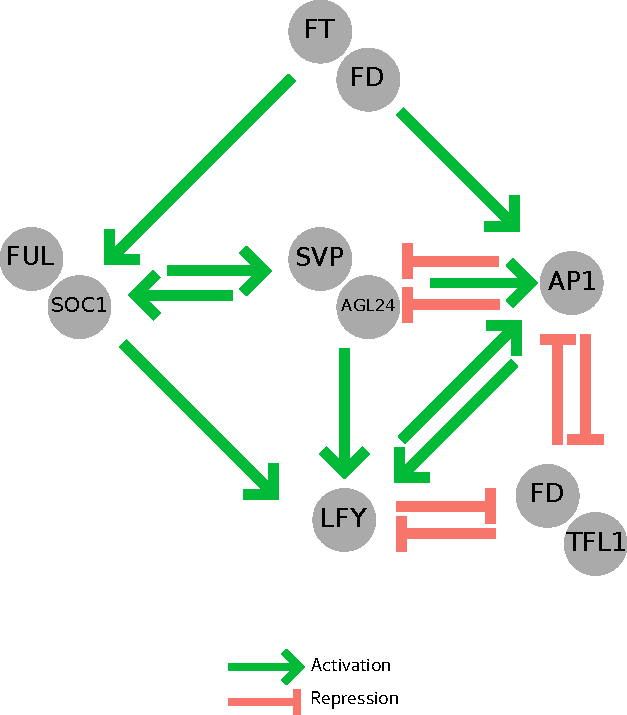
\includegraphics{figuredirectory/gene_regulatory_network.pdf}
\caption{\textbf{The core network of floral integrators.}}{Many
regulatory interactions have been found between the nine floral
integrators depicted here. This results in a tightly interconnected gene
regulatory network, with many possible feedback loops and control
mechanisms. Adapted from Bouché et
al.\textsuperscript{288}}\label{figure:1xx:floralnetwork}
\end{figure}

The pathways described above converge onto a set of floral integrator
genes, that mediate the transition to flowering. The core of this
network is composed of relatively few transcription factors with
multiple regulatory links between them. These feedback loops allow for
the signals from the flowering time pathways to be appropriately
interpreted and provide robustness to the system\textsuperscript{38}.

Both the photoperiod and vernalization pathways converge onto the
expression of the floral activator \emph{FT}. Grafting experiments in a
number of plant species led to the conclusion that a floral inducer,
referred to as the florigen, was transported from leaves to the shoot
apex to initiate flowering\textsuperscript{39,40}. It later emerged that
the florigen, initially hypothesised to be a plant hormone, was the
protein FT. \emph{FT} is expressed in the phloem companion cells, and
the FT protein is transported in the plant vasculature from leaves to
the apex to promote flowering\textsuperscript{41--43}. The gene was
identified from a photoperiod sensitive mutant plant that exhibited
delayed flowering when the plants were grown in long
days\textsuperscript{32}. This photoperiod sensitivity was found to be
due to \emph{FT} being directly regulated by the circadian clock gene
\emph{CO}\textsuperscript{20--22}. The vernalization pathway also
influences the expression of \emph{FT}, with \emph{FLC} binding to a
site within the first promoter of \emph{FT} to repress its
expression\textsuperscript{44}. \emph{FT} activates the expression of
three MADS-box containing proteins that promote flowering;
\emph{FUL}\textsuperscript{45}, \emph{SOC1}\textsuperscript{46}, and
\emph{AP1}\textsuperscript{47}. These will be discussed in more detail
later in this section.

A gene found to act in an antagonistic manner to \emph{FT} in
determining the floral transition is \emph{TERMINAL FLOWER 1}
(\emph{TFL1}). Wild type Arabidopsis flowers develop in an indeterminate
manner\textsuperscript{48}. When the transition to flowering occurs, the
vegetative meristem converts into an inflorescence meristem that in turn
generates the floral structure. Additional inflorescence meristems, and
eventually floral meristems, develop on the side of the main
inflorescence stem. However, the shoot apical meristem, located at the
top of the floral structure, remains as an inflorescence meristem, and
hence floral growth is indeterminate in Arabidopsis. Mutants in
\emph{TFL1} result in the primary inflorescence meristem converting into
a floral meristem, such that the floral structure terminates in a flower
as opposed to maintaining an indeterminate state\textsuperscript{49}. In
addition, \emph{TFL1} null mutant plants also undergo the floral
transition earlier than wild type plants\textsuperscript{50}.
\emph{TFL1}, therefore, is a repressor of the floral state, influencing
meristem identity and regulating the timing of the floral transition.
The inflorescence meristem identity is maintained by TFL1 protein
through limiting the activity of \emph{AP1} and
\emph{LFY}\textsuperscript{51--53}. In addition to transcriptional
repression, TFL1 protein also limits the activity of AP1 and LFY, as
shown by Arabidopsis lines that overexpressed \emph{TFL1} and either
\emph{AP1} or \emph{LFY}\textsuperscript{53}. Likewise, \emph{AP1} and
\emph{LFY} repress \emph{TFL1}, with the mutual antagonism likely
leading to the sharp expression boundaries required to accurately
specify floral development\textsuperscript{51,54} \emph{TFL1} and
\emph{FT} are very closely related proteins, with only 39 amino acid
changes that distinguish the two proteins\textsuperscript{55}. Indeed,
mutations have been found that produce TFL1 proteins that are FT-like
and vice versa\textsuperscript{55--57}.

Despite being central floral integrators, both \emph{FT} and \emph{TFL1}
do not possess DNA binding activity themselves and are therefore not
transcription factors. Instead, the proteins of both genes interact with
the FD protein, a bZIP transcription factor\textsuperscript{38,45,47}.
\emph{FD} was originally identified as a late flowering
mutant\textsuperscript{32} found to repress the phenotype of \emph{FT}
overexpression lines\textsuperscript{47}. The FD protein was confirmed
as an interacting partner of FT in a yeast-two hybrid
screen\textsuperscript{45}, and was found to also bind FT \emph{in
vitro}\textsuperscript{47}. Two lines of evidence point towards FT and
FD interacting to promote \emph{AP1} expression. The first is the
ectopic expression of \emph{AP1} observed in \emph{FD} overexpression
lines that is dependent on the presence of
\emph{FT}\textsuperscript{47}. The second line of evidence are chromatin
immunoprecipitation experiments in an \emph{FD} overexpression line.
Antibodies for the FT protein were used to enrich DNA and \emph{AP1}
promoter sequence was found\textsuperscript{45}.

A homeotic mutation in Arabidopsis that severely impacts the transition
from vegetative to floral growth is in the \emph{LEAFY} (\emph{LFY})
gene. \emph{LFY} was identified in a mutant screen as a mutant that
produced leafy shoots in the place of flowers, with the flowers produced
often lacking petals and stamens\textsuperscript{58}. The gene was found
to play a role both in the transition to flowering, but also in
specifying the determinacy of the floral meristem\textsuperscript{59}.
LFY binds to DNA as a dimer, with the cooperative nature of this binding
suggested to facilitate a sharp developmental
transition\textsuperscript{60}. \emph{LFY} has been found to regulate or
interact with a number of other genes involved with the floral
transition. Increasing \emph{LFY} expression precedes an increase in
\emph{AP1} expression\textsuperscript{61}, with additional evidence
suggesting that \emph{AP1} is a direct target of
\emph{LFY}\textsuperscript{62,63}. Other genes important for flowering
that are regulated by \emph{LFY} are \emph{TFL1}\textsuperscript{64},
\emph{AG}\textsuperscript{65,66}, and \emph{CAL}\textsuperscript{63},
with \emph{LFY} itself being regulated by \emph{SOC1} and
\emph{AGL24}\textsuperscript{67}. In addition, a suite of transcription
factors and signalling molecules, both related to flowering time and
not, were found to respond to \emph{LFY} activation or have \emph{LFY}
binding detected in promoter regions\textsuperscript{63,68}.
Interactions between \emph{LFY} and the photoperiod
pathway\textsuperscript{69}, and the GA pathway\textsuperscript{70,71},
suggest that many environmental pathways that regulate flowering
converge on \emph{LFY}, underpinning its role as a floral integrator.

\emph{AP1} is a MADS-box containing transcription
factor\textsuperscript{72} important for both controlling meristem
identity and floral organ specification. Null mutations in the
\emph{AP1} gene result in the mutant plants lacking
petals\textsuperscript{73}, a consequence of the role \emph{AP1} has in
specifying floral organ identity. Additionally, the sepals that usually
surround flowers in \emph{AP1} mutant plants are instead converted to
bracts, with secondary flower buds formed in the axils of each
bract\textsuperscript{74}. This particular phenotype suggests that
\emph{AP1} is important for the conversion of the inflorescence meristem
into a floral meristem, as without an active version of the \emph{AP1}
protein the floral meristem partially reverts back to an inflorescence
meristem\textsuperscript{72}. This is also supported by the \emph{AP1}
overexpression phenotype, where apical and lateral shoots are converted
into flowers\textsuperscript{75}. The modulation of meristem activity by
\emph{AP1} is believed to be via the plant hormone cytokinin, with
\emph{AP1} affecting both the biosynthesis and degradation pathways of
the hormone\textsuperscript{76}. 25~\% of the putative targets of
\emph{AP1} are other transcription factors, such as \emph{LFY},
explaining why mutants and overexpressors of \emph{AP1} have such
dramatic effects on flower development in
Arabidopsis\textsuperscript{77}. \emph{AP1} and \emph{LFY} double null
mutants had a significantly more severe phenotype than either of the
single mutants, indicating that these genes seem to act
synergistically\textsuperscript{78}. In mutant plants lacking
\emph{AP1}, \emph{SHORT VEGETATIVE PHASE} (\emph{SVP}), \emph{AGL24},
and \emph{SOC1} become ectopically expressed\textsuperscript{79}, with
further evidence suggesting that \emph{AP1} directly represses the
expression of these genes\textsuperscript{80}. \emph{SVP} and
\emph{AGL24} maintain the vegetative and inflorescence meristems
respectively\textsuperscript{79}. The expression of \emph{AP1} therefore
confers a floral state to the meristem.

A gene involved with integration of inputs from an array of different
flowering time pathways is \emph{SOC1}\textsuperscript{81}. The gene was
discovered\textsuperscript{82} and rediscovered\textsuperscript{83} in
Arabidopsis through a number of different experimental methods. The
\emph{SOC1} gene was found to be differentially expressed after
activation of an inducible CO protein in the absence of protein
translation, suggesting \emph{SOC1} is a direct target of
CO\textsuperscript{20} and thus downstream of the photoperiod pathway.
Indeed, \emph{SOC1} gets its name as a mutant in the \emph{SOC1} gene
was able to suppress the early flowering phenotype of an Arabidopsis
line overexpressing \emph{CO}\textsuperscript{82}. The overexpression of
\emph{SOC1} in a vernalization requiring line of Arabidopsis was able to
overcome the vernalization requirement, suggesting that \emph{SOC1} also
is also a part of the vernalization pathway\textsuperscript{83}.
Subsequent analysis has revealed that this regulation is likely to be
direct, as a transcription factor motif in the \emph{SOC1} promoter was
found to be bound by FLC \emph{in vitro} and required for \emph{SOC1}
repression \emph{in vivo}\textsuperscript{44,84}. \emph{SOC1} was
initially discovered, therefore, as acting downstream of the
vernalization and photoperiod flowering pathways, and subsequent
investigations have revealed that \emph{SOC1} is involved with
additional floral pathways. The rescue of a GA biosynthesis mutant with
the treatment of GA causes an increase in the expression of
\emph{SOC1}\textsuperscript{85}. This finding, in addition to the
\emph{SOC1} mutant being less sensitive to the treatment of
GA\textsuperscript{85}, suggests \emph{SOC1} integrates the response to
the GA-dependent, hormonal pathway. \emph{SOC1} has also been implicated
in the intermittent cold-sensing pathway\textsuperscript{86} and the
age-dependent flowering pathway\textsuperscript{87}. All this evidence
points towards \emph{SOC1} being a central integrator that is the
convergence point of a range of flowering time control pathways.

The regulation of \emph{SOC1} is tied to another MADS-box containing
flowering time gene, \emph{AGL24}, as both regulate each other in a
positive feedback loop\textsuperscript{88}. The AGL24 protein was found
to be important for the entry of SOC1 protein into the nucleus, with
AGL24 and SOC1 binding as a probable dimer at the promoter of
\emph{LFY}\textsuperscript{67}. \emph{AGL24} seems to act somewhat
redundantly with \emph{AP1} and \emph{SVP} to repress certain genes
involved with floral organ specification to properly pattern the
developing flower\textsuperscript{89}.

The \emph{SOC1} gene is at least somewhat redundant with the gene
\emph{FUL}, suggesting that \emph{FUL}\textsuperscript{90}, and like
\emph{SOC1} is activated by \emph{FT} expression\textsuperscript{91}.
The gene was characterised as affecting the development of the
Arabidopsis seed pod\textsuperscript{92}, but was also found to act
earlier in the reproductive phase by controlling flowering time and
meristem identity alongside \emph{AP1} and
\emph{SOC1}\textsuperscript{93}. Indeed, plants that are mutant in both
\emph{FUL} and \emph{SOC1} remain vegetative, and almost resemble
perennial plants\textsuperscript{90}. SOC1 and FUL
interact\textsuperscript{94}, and have been found to bind to and
activate \emph{LFY} expression\textsuperscript{95}.

Finally, \emph{SVP} is a gene that seems to have a dual role as a floral
repressor early in development, and as floral meristem identity
specification gene later in development, with differing target
genes\textsuperscript{96}. As a floral repressor, it has been found to
form a heterodimer with FLC, although lack of SVP does not significantly
impact the targets of FLC. This is not mutual, however, as the presence
of FLC causes a large effect on the targets of SVP, with the number of
targets doubling\textsuperscript{97}. As with FLC, SVP has been found to
bind at the \emph{FT} locus to delay the floral
transition\textsuperscript{98}. When the floral transition occurs,
however, the gene product seems to act redundantly with AP1, AGL24, and
SOC1 to maintain an indeterminate
meristem\textsuperscript{80,89,99,100}. Extensive heterodimer formation
has been demonstrated between the MADS-box containing flowering time
gene products\textsuperscript{94}. It therefore seems likely that the
role of \emph{SVP} changes depending on which genes it dimerizes
with\textsuperscript{80,97}.

Being sessile organisms, plant need to interpret environmental cues and
respond appropriately. The different floral pathways allow for these
environmental cues, and for endogenous cues such as age, to be
interpreted. The combined interactions of the floral integrators
discussed here allow for these signals to be combined provide robustness
to the floral transition\textsuperscript{38}. The flowering time genes
and pathways identified in Arabidopsis have been found to be somewhat
conserved in a wide range of crop species\textsuperscript{3}, leading
some to dub Arabidopsis the `Rosetta stone' of flowering time
research\textsuperscript{101}.

\section{\texorpdfstring{The origin of \emph{Brassica napus} and why
flowering time is
important}{The origin of Brassica napus and why flowering time is important}}\label{section:intro:brassica}

The \emph{Brassica} genus is in the same taxonomic family as
Arabidopsis, the Brassicaceae\textsuperscript{102}, and comprises a
large number of economically important vegetable and oil crops that show
broad morphological divergence. Among the \emph{Brassicas} are both
diploid and tetraploid species. Diploid species of the \emph{Brassica}
genus include \emph{B. rapa} (Chinese cabbage, turnip, and pak choi),
\emph{B. oleracea} (kale, cabbage, broccoli, cauliflower, and Brussels
sprout), and \emph{B. nigra} (black mustard). A theory proposed by Woo
Jan-choon in 1935, that has become known as the triangle of U, posits
that ancestors of the above diploid species hybridized to give ancestors
of the tetraploid species of \emph{Brassicas}. These tetraploid species
are \emph{B. napus} (oilseed rape, swede, kale), \emph{B. carinata}
(Ethiopian mustard), and \emph{B. juncea} (Indian mustard). As the
tetraploids are the result of interspecies hybridization events they are
termed allopolyploids. Progenitors to modern day \emph{B. rapa} and
\emph{B. oleracea} plants are thought to have hybridized to form
ancestral \emph{B. napus} less than 10,000 years
ago\textsuperscript{103}, with multiple hybridizations having taken
place to give the modern \emph{B. napus} gene pool\textsuperscript{104}.
Rapeseed crops such as \emph{B. napus}, are the second most cropped oil
crop worldwide comprising 13~\% of the total yield\textsuperscript{105},
with the oil being used as a vegetable oil and for industrial
lubricants. In the UK, 13~\% of the total area on which crops were grown
in 2016 (608,000 hectares) were used for oilseed crops, generating £541
million in income\textsuperscript{106}. Wheat grown following oilseed
rape will yield 10~\% more than a wheat grown continuously, on
average\textsuperscript{107}.

\begin{table}[htp]
\caption{\textbf{Main \emph{Brassica} crops, their common names, and the part of the plant that is consumed.}}{ Table obtained from Cartea et al.[TODO]}
\label{intro:table1xx:brassicas}
\centering
\resizebox{\textwidth}{!}{%
\begin{tabular}{llll}
\toprule
Species & Group & Common name & Organ consumed \\
\midrule
\emph{Brassica oleracea} & \emph{acephala}          & Kale, collards           & Leaves \\
                         & \emph{capitata capitata} & Cabbage                  & Terminal leaf buds (heads) \\
                         & \emph{capitata sabauda}  & Savoy cabbage            & Terminal leaf buds (heads) \\
                         & \emph{costata}           & Tronchuda cabbage        & Loose heads \\
                         & \emph{gemmifera}         & Brussels sprouts         & Vegetative buds \\
                         & \emph{botrytis botrytis} & Cauliflower              & Inflorescences \\
                         & \emph{botrytis italica}  & Broccoli                 & Inflorescences \\
                         & \emph{gongylodes}        & Kohlrabi                 & Stem \\
                         & \emph{albogabra}         & Chinese kale             & Leaves \\
\emph{Brassica rapa}     & \emph{rapa}              & Turnip                   & Roots \\
                         & \emph{rapa}              & Turnip greens            & Leaves \\
                         & \emph{rapa}              & Turnip tops              & Shoots \\
                         & \emph{chinensis}         & Pak choi, bok choi       & Leaves \\
                         & \emph{pekinensis}        & Chinese cabbage, pe-tsai & Leaves \\
                         & \emph{parachinensis}     & Choy sum                 & Leaves \\
                         & \emph{ruvo}              & Broccoleto               & Shoots \\
                         & \emph{perviridis}        & Komatsuna, Tendergreen   & Leaves \\
\emph{Brassica napus}    & \emph{pabularia}         & Leaf rape, nabicol       & Leaves \\
                         & \emph{napobrassica}      & Swede                    & Roots \\
\emph{Brassica juncea}   & \emph{rugosa}            & Mustard greens           & Leaves \\
                         & \emph{capitata}          & Head mustard             & Heads \\
                         & \emph{crispifolia}       & Cut leaf mustard         & Leaves \\
\bottomrule
\end{tabular}%
}
\end{table}

Aside from being an economically important crop, the \emph{Brassica}
species are also a model for gene retention. The genomes of
\emph{Brassica} species have undergone genome duplication events
relative to \emph{Arabidopsis} since the two genera diverved 43 million
years ago\textsuperscript{108}. There is evidence for an ancestor of the
\emph{Brassica} lineage being a hexaploid, with estimates of when the
genome triplication occurred varying from 7.9 - 14.6 million years
ago\textsuperscript{109} and 23 million years ago\textsuperscript{108}.
Subsequent diploidization of this hexaploid ancestor has given us the
diploid \emph{Brassica} species we have today. \emph{B. rapa} and
\emph{B. oleracea} diverged 0.12 - 3.7 million years
ago\textsuperscript{110,111}, with the process of chromosome
rearrangement resulting in a chromosome number of 10 for \emph{B. rapa}
(A genome)\textsuperscript{112} and 9 for \emph{B. oleracea} (C
genome)\textsuperscript{113}. It is thought that the interspecies
hybidization event resulting in the allopolyploid \emph{B. napus}
occurred less than 10,000 years ago\textsuperscript{103}. Both the
ancient hexaploid state of the \emph{Brassica} genomes and the
interspecies hybridization event mean that \emph{B. napus} has a greatly
increased gene number than Arabidopsis (101,040\textsuperscript{114}
relative to 25,498\textsuperscript{10}), with genes in Arabidopsis often
having multiple homologues in the \emph{B. napus} genome. Despite large
scale genome rearrangements, extensive collinearity between the
\emph{Brassica} and Arabidopsis genomes
remains\textsuperscript{112--114}. This genomic collinearity and
relatedness of the two plant species has been exploited to translate
research from the model plant to the crop species, as well as
investigate the effects of gene duplication.

\subsection{\texorpdfstring{How does flowering time affect the
cultivation of \emph{Brassica}
species?}{How does flowering time affect the cultivation of Brassica species?}}\label{how-does-flowering-time-affect-the-cultivation-of-brassica-species}

The success of many \emph{Brassica} crops is dependent on their
flowering time. The edible componant of both broccoli (\emph{B. rapa}
var. \emph{botrytis italica}) and cauliflower (\emph{B. rapa} var.
\emph{botrytis botrytis}) are the plant inflorescences, and the timing
of the floral transition and floral development in general is very
important for these crops as a consequence. Using variation in curd
formation in cauliflower, a number of potential candidate genes were
identified as controlling the response to temperature, with some of
these genes being homologues of floral genes in
Arabidopsis\textsuperscript{115}. With other \emph{Brassica} crops, such
as Chinese cabbage (\emph{B. rapa} var. \emph{pekinensis}) the
prevention of flowering is desired. Chinese cabbage is grown for its
leaves (Table \ref{intro:table1xx:brassicas}). If the plant transitions
to floral growth, it will bolt, significantly reducing its economic
value. The expression of a floral repressor, a \emph{B. rapa} homologue
of \emph{FLC}, was found to correlate with bolting time in different
Chinese cabbage lines\textsuperscript{116}.

\emph{B. napus} crops are predominantly used as oilseed crops, in which
the timing of the floral transition impacts both when the seed filling
period begins and how long it progresses. Indeed, the interconnected
nature of yield and flowering has been suggested by association studies
finding regions of the genome associated with both
traits\textsuperscript{117,118}. The yield of oilseed rape crops is
determined by the number of seeds the plants produce per area and the
weight of each seed. Numbers of pods and seeds are largely determined
during a 3 week phase after flowers have
formed\textsuperscript{119,120}, with the quality of the seed dependent
on a period of seed filling. The seed quality is related to temperature,
with cooler conditions extending seed filling, and the rate of
photosynthesis, with the majority of oil in the seed accumulated during
the second half of seed filling\textsuperscript{120}. The effect of
photosynthesis during the seed filling period is potentially of greater
significance in \emph{B. napus} relative to other crops as the
remobilization of carbohydrates accumulated before flowering is
\textasciitilde{}12~\%, compared to 20~~-50~\% in
wheat\textsuperscript{120,121}. Yield of winter oilseed rape has been
found to be related to the size of the crop at
flowering\textsuperscript{119}. This is in turn a function of the length
of time between the beginning of spring, when mean growing temperatures
exceeded 5 °C, and when the plants flowered in late May. Therefore, the
highest yielding years were those where spring was early and flowering
late, allowing the longest period of time for growth in this critical
period. Similar findings came out of modelling the growth of \emph{B.
napus}, with higher yields predicted to be obtained by delaying plant
maturity and promoting earlier flowering, to ensure the seed filling
period is as long as possible\textsuperscript{122} Therefore, when
flowering occurs during the growing season, and how that relates to the
climate in which the crop is grown, can heavily influence the yield and
quality of the crop.

Whether the oilseed rape is a spring or winter variety is also
important, as different growing regions require different types of crop.
In Europe and Asia, winter oilseed rape is predominantly grown, whereas
in Australia, Canada, and northern Europe spring types are generally
grown\textsuperscript{123}. For Canada and northern Europe, the
requirement for spring types results form harsh winters that prevent the
crop from being overwintered. Therefore, the vernalization requirement
of a variety is important to consider for the planned crop rotation a
particular farmer or growing region requires. Additionally, the length
and severity of cold required by a variety will dictate whether that
variety is suitable to a particular application.

Finally, the availability of pollinators can significantly impact the
yield of \emph{B. napus} crops. Preventing pollinators visiting winter
oilseed rape plants led to a 27~\% decrease in the number of seeds
produced and a 30~\% decrease in the seed weight per
pod\textsuperscript{124}. In addition the diversity of those pollinators
visiting the plants is related to oilseed rape
yield\textsuperscript{125}. Changes to flowering time will affect the
pollinators that are available to the flowering plants. This has been
found to profoundly affect the reproductive success of perennial
wildflowers\textsuperscript{126}. Therefore, as the yield of oilseed
rape is influenced by pollinator availability\textsuperscript{124,125},
the correct timing of flowering is required.

\subsection{Work on the control of flowering in Brassica
species}\label{section:intro:brassicafloweringgenes}

Extensive work on how the floral response is controlled in Arabidopsis
has facilitated understanding of floral control in a range of crop
plants\textsuperscript{3}. Homologues of the floral genes (section
\ref{section:intro:arabidopsis}) have been detected in the genomes of
\emph{Brassica} species, which due to the gene multiplication events
that have occurred in the Brassica lineage are often present as multiple
copies\textsuperscript{127}. However, identification of whether these
\emph{B. napus} homologues have similar functions to their counterparts
in Arabidopsis, and of functional differences between the homologues, is
often lacking.

Likely as a result of both spring and winter varieties of
\emph{Brassica} crops being of such economic value, the vernalization
pathway has arguably been the most well studied flowering pathway in
Brassicas. Association studies focussing on mapping the vernalization
response in \emph{B. rapa}\textsuperscript{128--133}, \emph{B.
oleracea}\textsuperscript{132,134--136}, and \emph{B.
napus}\textsuperscript{130,137--139} have identified regions containing
homologues of \emph{FLC} and \emph{FRI} as explaining flowering time
variation. These homologues exhibit similar decreases in expression
during cold as their Arabidopsis counterpart\textsuperscript{116,140}
and have been investigated to determine if they have diverged in
function or not. Expression of five different \emph{FLC} homologues in
Arabidopsis conferred a vernalization requirement in a rapid-cycling
accession of Arabidopsis\textsuperscript{141}. Interestingly, the delay
in flowering as a result of the transgenic gene varied depending on the
homologue, suggesting that the genes have diverged roles in \emph{B.
napus}\textsuperscript{141}. The results from association studies
carried out with different mapping populations have also suggested that
the \emph{FLC} copies in \emph{Brassicas} have diverged, with the copies
on chromosomes A10 and A2 having stronger associations with flowering
time\textsuperscript{133,137}. Similarly, multiple \emph{FLC} homologues
from \emph{B. rapa} delayed flowering when overexpressed in both
Arabidopsis and Chinese cabbage, suggesting a conservation of
function\textsuperscript{142}. \emph{FRI} homologues from \emph{B.
oleracea} were able to complement an Arabidopsis accession that contains
a nonfunctional copy of the gene\textsuperscript{143}, indicating
conservation of function. Despite all homologues being able to
complement Arabidopsis, structure of the \emph{FRI} homologues from
\emph{B. oleracea} have diverged with alterations in the number of
coiled-coil domains, potentially impacting protein-protein
interactions\textsuperscript{143}. Therefore, although it has been
established that \emph{FLC} and \emph{FRI} seem to be important in the
vernalization pathways of both \emph{Brassica} crops and
Arabidopsis\textsuperscript{27}, how the copies of these genes have
diverged in \emph{Brassica} is only beginning to be understood.

Genes in other flowering time pathways, and the floral integrators, have
also been investigated in \emph{Brassica} species. Genes involved with
the circadian clock have been retained in the \emph{B. rapa} genome,
suggesting that the dosage of the genes is important for their
function\textsuperscript{144}. In particular, homologues of the clock
sensitive gene \emph{CO} are associated with changes in flowering time
in both \emph{B. oleracea}\textsuperscript{145} and \emph{B.
nigra}\textsuperscript{146,147}. Homologues of \emph{TFL1} were
identified in \emph{B. rapa}, \emph{B. oleracea}, and \emph{B. napus},
with expression in the flower in the latter species in line with
expression of the gene in Arabidopsis\textsuperscript{148}. Mutations in
the A10 copy of \emph{TFL1} in \emph{B. napus} caused a delay in
flowering, affected internode elongation, and resulted in an increase in
seed number and weight\textsuperscript{149}. Homologues of \emph{FT} in
\emph{B. napus} exhibited different expression patterns, with certain
copies having a stronger effect on flowering than
others\textsuperscript{149}. Expression differences were observed
between the homologues of \emph{FT} in \emph{B. rapa}, \emph{B.
oleracea}, and \emph{B. napus}\textsuperscript{150}. Within \emph{B.
napus}, one copy was silenced as a result of transposon insertion into
the promoter region and the expression of another two copies was crop
type specific\textsuperscript{150}. Transposon mediated changes to the
expression of an \emph{FT} homologues were also identified in \emph{B.
rapa}, resulting in flowering time differences. This suggested that this
copy of \emph{FT} has retained a function similar to its counterpart in
Arabidopsis\textsuperscript{151}. Arrest of floral development is
required in broccoli and cauliflower to form the heads correctly.
Interestingly, the floral genes predicted to cause the arrest
(\emph{LFY}, \emph{AP1}, and \emph{TFL1}) were not implicated, causing
the authors to suggest other floral meristem genes are mediating the
change relative to Arabidopsis\textsuperscript{152}. Links between
flowering time and \emph{SOC1} homologues have been identified in
\emph{B. rapa}\textsuperscript{153}, with expression differences
detected between the different homolgoues in \emph{B. rapa} and \emph{B.
juncea}\textsuperscript{153,154}.

Despite evidence of flowering time genes homologues having similar roles
in \emph{Brassica} species, in-depth analysis of how different
homologues are behaving is often lacking. This is not the case for all
genes however, with the roles of \emph{FT}, \emph{FLC}, and \emph{FRI}
homologues in \emph{Brassica} species being dissected in a copy specific
manner\textsuperscript{137,138,143,150}. These investigations have
revealed that individual copies have indeed diverged in function and
behaviour.

\section{Modelling flowering time and
crops}\label{modelling-flowering-time-and-crops}

From simulating cell-signalling dynamics\textsuperscript{155},
patterning of biological systems\textsuperscript{156}, up to population
level models\textsuperscript{157}, mathematical models have been able to
capture the behaviour of a range of biological processes. Models allow
researchers to collect potentially disparate observations together to
test if they are consistent with each other. If they are consistent,
then the researchers' assumptions about the system are compatible with
the data and the model can be used to make predictions. If the model
does not capture the behaviour of the system, then clearly the system is
more complex than originally thought. Either way, modelling systems can
direct future research work and highlight features of the system that
might not have been appreciated had a reductionist approach had been
taken. This section will highlight models of the floral transition that
have been developed, as well as how models of crop growth have been used
by both the agricultural industry and scientific community to direct
scientific effort and farming practises.

\subsection{Models of the floral
transition}\label{models-of-the-floral-transition}

The floral transition is composed of a suite of transcription factors
that control the floral development both spatially and temporally
(section \ref{section:intro:floralintegrators}). As the regulatory
interactions between these transcription factors have been elucidated,
gene regulatory networks have been used to model the floral
transition\textsuperscript{38,158}. Gene regulatory networks consist of
genes as hubs in the network and the regulatory interactions between
those genes as edges of the network\textsuperscript{159}. The genes
involved in these networks generally encode transcription factors;
proteins that have the capacity to alter the transcription of other
genes. The network structure results as a consequence of regulatory
links between transcription factors. The combination of interactions
between transcription factors can lead to complex behaviours that have
favourable properties such as noise cancellation, high-pass filters, and
low-pass filters\textsuperscript{160}. The combination of these, and
other, simple regulatory structures allows for complex responses to
stimuli to be encoded\textsuperscript{161}.

As a consequence of their capacity to capture complex behaviours between
genes, gene regulatory networks have been employed in many fields of
biology\textsuperscript{162}. The behaviours captured by the models, and
the consequences of those behaviours such as noise cancelling or signal
amplification, are often initially unintuitive, highlighting the
necessity of the models\textsuperscript{160}. An example of particular
interest to the work presented here is that of Jaeger et al. (2013), in
which the floral transition was modelled\textsuperscript{38}. A
simplified network of five floral integrators, \emph{FT}, \emph{SOC1},
\emph{FD}, \emph{TFL1}, and \emph{AP1} were used as hubs in the network,
with edges consisting of regulatory interactions determined genetically
and molecularly (section \ref{section:intro:floralintegrators}). The
model consisted of five gene hubs and was parameterized using the
flowering time (measured as the number of rosette and cauline leaves
present at flowering) of Arabidopsis single and double mutants in the
floral integrators. The model was able to capture a number of dynamics
of the floral transition, such as irreversibility and noise filtering.
Insights from the model included the observation that the relative
levels of \emph{TFL1} and \emph{FT} were important for determining when
the floral transition occurred. Additional regulatory interactions
involving the regulation of \emph{TFL1} were also proposed as necessary
for the maintenance of a high \emph{TFL1} expression
state\textsuperscript{38}.

Valentim et al. (2015) extended the model of Jaeger et al. (2013) by
incorporating additional genes and by using expression data to
parameterize the model\textsuperscript{158}. This meant that, unlike the
gene hubs used in the earlier study, the genes in the Valentim et al.
model better corresponded to the genes themselves. The findings of the
study highlight the sometimes unintuitive dynamics that are unveiled
when a system is computationally modelled. For example, it was found
that mutating \emph{SOC1} has a greater effect on the expression of
\emph{AP1} than on \emph{LFY}, which is surprising given that the
regulation is indirect and direct respectively.

Although much more simplified than other modelling strategies, a two
gene regulatory model of the floral transition in a perennial relative
of Arabidopsis, \emph{Arabidopsis halleri}, was capable of accurately
modelling the floral transition and the timing of floral reversion back
to vegetative growth\textsuperscript{163}. By incorporating temperature
responsive production and degradation rates of the two genes into the
model, the projected effects of climate change on the developmental
timings of natural populations of the plants could be predicted.

The model developed by Espinosa-Soto et al. (2004) models a regulatory
network of 15 genes involved with the ABCE model of floral
patterning\textsuperscript{164}. Instead of modelling the expression
level of genes as continuous variables, as the other models have done,
discrete gene expression levels were used. This simplification allowed
the researchers to test every possible initial condition for their
model. The properties of the network resulted in the expression of the
genes converging to only 10 stable states, which corresponded to the
expression profiles of different floral cell lineages in the Arabidopsis
flower. In addition, the model was capable of reproducing regulatory
effects of knockout and overexpression
mutations\textsuperscript{164,165}.

Extending gene regulatory network based models away from model species,
Dong et al. (2012) developed a four gene regulatory model that took
structural cues from the network in Arabidopsis to model the floral
transition in maize\textsuperscript{166}. As with the Jaeger et al.
Arabidopsis model, this maize model was parameterized using total leaf
number as proxy measurement for flowering time, and validated using
mutants in the genes involved in the network.

All of these examples illustrate the insights that can be obtained from
taking into account the regulatory networks that underlying the floral
transition.

\subsection{Models of crop growth and yield
prediction}\label{models-of-crop-growth-and-yield-prediction}

Crop models have been studied and used in the research community for
over fifty years\textsuperscript{167}. These models aim to explain, or
predict, the growth of plant species that are grown as crops. The
motivation for using crop models can vary\textsuperscript{167}. For the
scientific community, crop models allow for the integration of seemingly
distinct models of processes. Initial models focussed on modelling
photosynthesis\textsuperscript{168} have been improved upon, with modern
models incorporating processes such as leaf development, light
interception, photosynthesis efficiency, and partitioning of biomass
within the plant\textsuperscript{169}. The other use of crop models is
to aid decision making, at a farm, country, and global
scale\textsuperscript{170,171}. Such models incorporate additional
processes such as nitrogen use efficiency\textsuperscript{172} and soil
erosion\textsuperscript{173}, in order to take into account the effect
of fertilizer use not only on the crop but to the wider
environment\textsuperscript{174,175}. The incorporation of climate and
weather data into these models have allowed predictions to be made about
the effects of climate change on crop growth and yield. Using this
methodology with multiple models allowed Rosenzweig et al. (2014) to
predict that low latitude areas would be most affected by climate change
in terms of crop yield for four different crop
types\textsuperscript{176}. Ultimately crop models at this scale can be
used to predict harvesting dates of some crops, allowing sowing dates to
be optimized and allowing the supply of the crop to be more accurately
estimated\textsuperscript{177}. For example, the use of climate
forecasting was used in the sugar industry to improve water use
efficiency at the farm level, while also benefiting industries further
down the sugar supply line through enhanced
scheduling\textsuperscript{178}.

Crop models can be split into two types; process-led models and
statistical models\textsuperscript{2,179,180}. In process led models,
the inputs to processes and how those outputs interact are explicitly
modelled, and are used to help understand plant-environment
interactions. The effects of changing inputs can be tracked through the
model, and stability analysis can be conducted to determine what input
parameters the model is particularly sensitive to\textsuperscript{181}.
The advantages of modelling processes explicitly is that, generally, the
predictions which the model can make are more accurate. Specifically,
the ability of the model to extrapolate and make predictions about
future events is improved by effectively giving the model an
understanding of how the crop plants under study will respond to
particular inputs\textsuperscript{2}. The downside of such models is
that they often have many parameters, that either have to be measured or
predicted from training sets of data. This parameterization often
requires a lot of data to be collected, which with crop plants may be
difficult or costly to do. The complexity of the models will also affect
how quickly these parameters can be estimated, and often how long the
model will take to run. Once trained, however, the insights from the
models can be very precise. Modelling wheat growth in sub-tropical India
found yields were very sensitive to temperature, potentially informing
the selection of future varieties grown\textsuperscript{181}. Modelling
the growth of maize, spring wheat, and soybean revealed that an altered
planting date combined with alternative varieties could reduce losses
due to projected climate change by 18~\%.

Statistical models, conversely, do not explicitly model processes, and
instead attempt to relate model inputs, such as climate data, to model
outputs, such as crop yield, in a correlative
manner\textsuperscript{182}. These models are much simpler, with fewer
parameters, than the process-led models. This means the models are
faster to run and potentially require less data to parameterize them.
This makes statistical models well-suited for use as summary models,
that capture the general trends between variables\textsuperscript{167}.
However, as the models do not interpret the data in terms of plant
growth, statistical models are potentially less accurate when
extrapolating the data to make predictions. Despite their simplicity,
statistical models are still capable of facilitating insight, such as
predicting potato yields from satellite imaging and remote sensing
data\textsuperscript{183}.

\subsection{Integrating the two types of
models}\label{integrating-the-two-types-of-models}

A potential short-coming of modelling plant growth responses using
models that do not simulate regulatory networks is that regulatory logic
may be lost. Different crop varieties and species are often incorporated
into crop models through parameter changes\textsuperscript{171,174}.
However, the regulatory logic of the crop models will remain unchanged.
For example, the output from two signalling pathways may be required
simultaneously to activate expression of a particular target pathway.
Genetic differences between varieties could potentially alter this
logic, resulting in the target pathway being activated if \emph{either}
input pathway is active. This could result from differences in promoter
binding sites between varieties. Implementing this change in logic, in
the APSIM framework for example, would require writing an alternative
module that integrated the responses from the input pathways in a
different manner\textsuperscript{171,184}.

Integrating gene regulatory networks into crop models would only be
beneficial for processes where the regulatory logic of the system is
important. For example, plant developmental processes that have
previously been modelled are the circadean
clock\textsuperscript{185--188}, auxin
signalling\textsuperscript{189--192}, floral organ
development\textsuperscript{164,193--195}, and the regulation of
flowering time by photoperiod\textsuperscript{196,197}. The gene
regulatory network modelling studies discussed in the previous section
required detailed information for the regulatory connections between
genes, and often large numbers of parameters had to be estimated. To
have such in-depth models for each regulatory pathway that can be
adequately modelled with gene regulatory networks would lead to a vast
increase in complexity for the crop models. This could be overcome by
using the more in-depth regulatory modules to help parameterize the
broader crop models, or identify changes in regulatory logic that will
influence the results of the model. Some genes may also have pleiotropic
effects, influencing multiple pathways. Ordinarily, with crop models
that have a modular structure\textsuperscript{184}, this would require
multiple parameters having to be changed in each of the modules the gene
plays a role. Being able to determine which genes are likely to exhibit
pleiotropic effects by their location in regulatory networks would allow
these parameters to be estimated together, or for those particular
modules to be more intimately linked in the model.

A number of the models discussed in the previous section were
parameterized or validated using plants that lack parts of the
regulatory network. Therefore, aspects of gene regulatory networks such
as the presence or absence of nodes and edges could be estimated from
both genome sequencing and transcriptome profiling. Sequencing of four
\emph{B. napus} varieties with varying flowering times and vernalization
requirements uncovered variation in flowering time genes that were
mapped onto regulatory networks\textsuperscript{127}. This revealed
which copies of the genes were likely to be causative of the phenotypes
displayed by the plants. The cost of sequencing now facilitates variety
specific genome sequences to be generated\textsuperscript{198}, as has
been done with Arabidopsis\textsuperscript{199}. Whereas crop models
currently require crop growth data in order to parameterize models to
particular varieties, future models may be able to combine sequencing
data with gene regulatory networks to aid the process of
parameterization. Regulatory networks therefore have the capacity to act
as a bridge to allow sequencing data to be incorporated into crop
models. The difficulty arises in translating knowledge of regulatory
networks elucidated in model organisms, the challenges of which will be
discussed in the following section.

\section{Challenges of knowledge transfer from Arabidopsis to
Brassicas}\label{challenges-of-knowledge-transfer-from-arabidopsis-to-brassicas}

The central challenge of moving gene regulatory networks from
Arabidopsis to \emph{B. napus} is a consequence of the genome
multiplication events that have occurred in the
crop\textsuperscript{103,108,109,114}. Genome multiplication events have
contributed to adaptive radiations\textsuperscript{200},
speciation\textsuperscript{201} and increases in organism complexity, as
a result of the additional copies of genes. The presence of additional
copies reduce the selective pressure on genes, allowing mutations to
occur in genes with limited phenotypic effect. Over time these mutations
can result in genes acquiring novel functions (neofunctionalization),
losing a subset of their original function (subfunctionalization), or
becoming nonfunctional\textsuperscript{202}. In this way, genome
multiplication events provide evolutionary `raw material'. A major
challenge when translating knowledge from Arabidopsis to \emph{B.
napus}, therefore, is to determine how copies of a gene have diverged,
and whether the function of the gene in the model plant can be used to
infer the function of genes in the crop.

\begin{figure}[htbp]
\centering
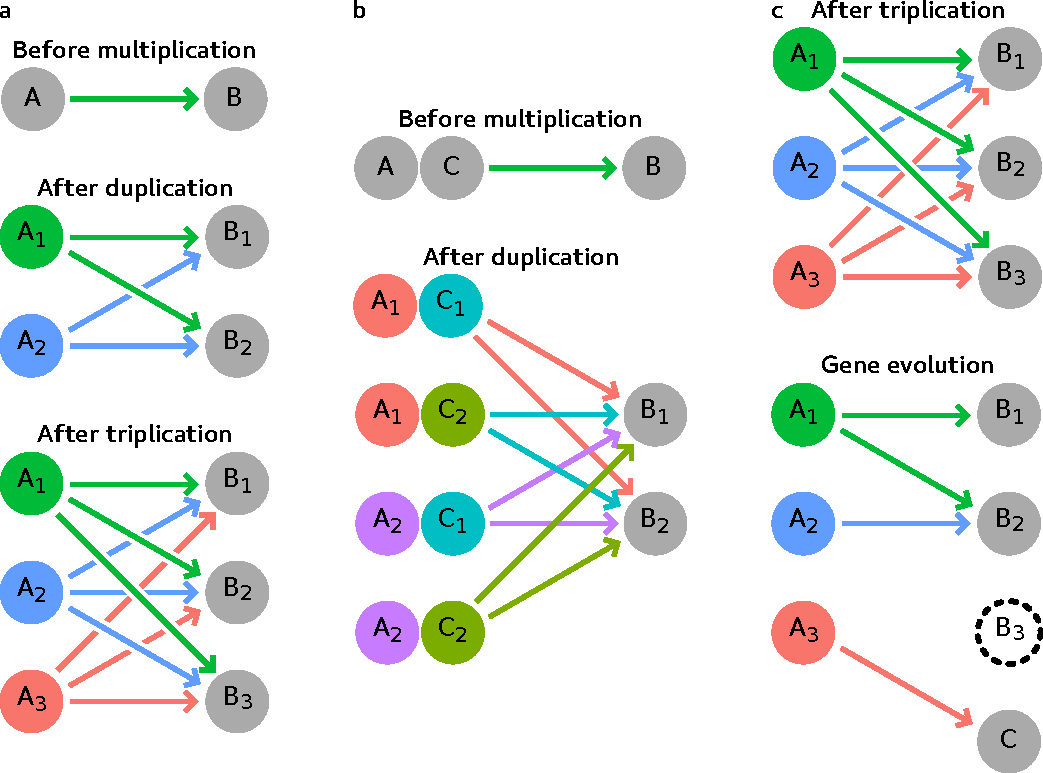
\includegraphics{figuredirectory/network_duplication.pdf}
\caption{\textbf{Whole genome multiplications lead to a vast increase in
the number of regulatory interactions.}}{\textbf{a} Regulatory links
(arrows) between transcription factors (A\textsubscript{x}) and their
targets (B\textsubscript{y}) increase in a quadratic manner following
successive multiplication events. \textbf{b} The increase in the number
of regulatory links is cubic for dimers, where A\textsubscript{x} and
C\textsubscript{z} are able to form dimers. \textbf{c} Over evolutionary
time, regulatory links may be lost (A\textsubscript{2} to
B\textsubscript{1}), novel regulatory links may form (A\textsubscript{3}
to C), and genes may be lost
(B\textsubscript{3}).}\label{figure:1xx:networkduplication}
\end{figure}

This problem is exacerbated when it comes to regulatory networks. If a
whole genome duplication occurs, not only is a transcription factor
present as multiple copies but so are its targets, leading to a huge
increase in the number of possible regulatory links. If we take the
total number of regulatory interactions present between genes in an
organism to be \(n\), a genome duplication event will cause this number
to increase to \(4n\). For a genome triplication, this number increases
to \(9n\) (Figure \ref{figure:1xx:networkduplication}a). In general, the
number of regulatory links after a genome multiplication event, assuming
no dimerization of transcription factors, will be \(nm^2\), where \(m\)
is the number of times the genome was multiplied. If the original
regulatory interaction before the multiplication involved a complex of
proteins as the regulator, however, the number of potential regulatory
interactions post-multiplication is greater than \(nm^2\). In the case
of dimers, using the same definitions of \(n\) and \(m\) as given above,
the increase in the number of regulatory links after a multiplication
event is \(nm^3\) (Figure \ref{figure:1xx:networkduplication}b). For a
complex of \(p\) proteins, the number of regulatory links present after
a multiplication event is \(nm^{(p+1)}\). Therefore, taking a regulatory
network elucidated in and validated using Arabidopsis and using it to
make predictions for \emph{Brassica} crops is problematic. Without
knowing which copies of genes have diverged in function and which have
retained their function, all copies of each gene would have to be used
in the model. The resulting model would be unwieldy to use and would
offer very little insight. It is therefore pertinent to understand how
copies of genes have diverged before using the regulatory network from
Arabidopsis to aid the construction of \emph{Brassica} regulatory
networks.

This thesis will investigate the divergence of gene copies in \emph{B.
napus} on a genome-wide scale, with a particular focus on the flowering
time genes. This was accomplished by generating a genome-wide
transcriptome dataset, collected before, during and after the floral
transition.

The first chapter explains how the data was collected and motivates the
experimental design decisions taken. Using only data from a spring
\emph{B. napus} variety, I reveal that flowering time genes have been
preferentially retained in the \emph{B. napus} genome. Widespread
divergence in the pattern of regulation between copies of homologous
genes suggests that this could have contributed to the observed
retention. An in-depth assessment of regulatory divergences between key
floral integrators is conducted. The chapter concludes with two case
studies investigating sequence divergence for \emph{B. napus} homologues
of \emph{TFL1} and \emph{FD}. In the case of \emph{TFL1}, the sequence
divergence correlates with regulatory divergence, whereas the sequence
divergence in \emph{FD} potentially influences the molecular function of
the gene.

The second chapter focusses on a winter variety of \emph{B. napus}. The
effects of a vernalization requirement on the global transcriptional
landscape are studied by assessing the extent of variety specific
expression. Regulatory divergence in the genes involved in the
vernalization pathway are assessed and compared to the expression of the
same genes in the spring variety. The comparison between a spring and
winter variety allows the vernalization response to be assessed for each
copy. Finally, the effects of a cold requirement for flowering on the
expression of floral integrators are studied to determine if certain
copies are more vernalization sensitive than others.

The final chapter details a web resource, created to allow the dataset
collected to be interrogated in a user-friendly and intuitive manner.
The dataset can be searched using Arabidopsis gene names to identify
\emph{B. napus} homologues and displays the expression patterns of these
homologues in both varieties and in both tissues sampled. Alternatively,
\emph{B. napus} genes can be searched using sequence homology. Although
flowering time genes are the focus of this thesis, the approach taken in
the first two chapters to assess regulatory divergence can be carried
out using any gene family. The creation of this website allows
researchers to study their own genes of interest without the need to
download large datasets or carry out laborious sequence alignment.

\chapter{Homologue divergence in a spring variety}\label{chapter:spring}

\section{Introduction}\label{section:spring_introduction}

The fate of duplicated genes following duplication has been studied in a
range of species\textsuperscript{203--206}, and in a range of
theoretical contexts\textsuperscript{207--212}. Ultimately, duplicated
genes need to provide an advantage to the organism or they will be
lost\textsuperscript{211}. Early discussions suggested that duplicated
genes become mutated and acquire novel, evolutionarily advantageous
functions, a process termed neofunctionalization\textsuperscript{207}.
However, as deleterious mutations occur more frequently than beneficial
mutations\textsuperscript{213}, under this model the expected rate of
gene retention following duplication is very low\textsuperscript{214},
with the majority of duplicated genes acquiring mutations that lead to
them being silenced\textsuperscript{208}. To account for this, the
duplication-degeneration-complementation (DDC)
hypothesis\textsuperscript{209}, posited that multiple copies of genes
are maintained through a partitioning of ancestral gene functions among
the duplicated genes, a process termed subfunctionalization. Another
method of subfunctionalization has been described as escape from
adaptive conflict\textsuperscript{212}. In this scenario, multiple
functions of a gene cannot be mutually optimized, with enhancement of
one function occurring at the detriment of the other. Upon gene
duplication, selection will favour each gene becoming adaptively
specialized to a particular function, leading to subfunctionalization.

A further method of gene retention in a genome following gene
duplication is gene redundancy. Redundancy can be defined as genetic
redundancy, in which gene loss is compensated for by another gene, or
functional redundancy, in which two genes may be functionally similar
but loss of one of the copies can still result in deleterious phenotypes
manifesting. Genetic redundancy led to the the idea of responsive backup
circuits, in which duplicated genes are retained in the genome to
provide robustness to gene loss, but also buffer against stochastic
effects during development\textsuperscript{215,216}. Functional
redundancy can be explained by the gene dosage hypothesis, which posits
that duplicate genes are retained to maintain gene
dosage\textsuperscript{210,217--220}. Such dosage effect may result if
the gene product acts as part of a protein complex, where an incorrect
stoichiometry of proteins can lead to deleterious
phenotypes\textsuperscript{218}. Interestingly the type of duplication
event is predicted to influence whether dosage effects result in gene
retention, or favour gene loss. The two main classes of gene duplication
event are small scale duplications and whole genome
duplications\textsuperscript{221,222}. After whole genome duplication
events the original protein stoichiometry is maintained. In this
scenario, selection will tend to retain dosage sensitive genes in the
genome\textsuperscript{218,220,223}. Conversely, small scale
duplications of dosage sensitive genes lead to incorrect protein
stoichiometry, leading to selection favouring gene
loss\textsuperscript{210}. Evidence from many species are consistent
with gene dosage effects maintaining duplicate genes in the
genome{[}224; blanc\_functional\_2004; seoighe\_genome\_2004{]}. An
interesting observation from these species, and from simulation
studies{[}maere\_modeling\_2005{]}, is that certain classes of genes are
found to be retained in the genome. This includes genes whose products
tend to form protein complexes, such as proteins involved with signal
transduction, transcriptional regulation, protein binding and
modification, and kinase activity. In \emph{Saccharomyces cerevisiae},
genes retained following whole genome duplication are also genes found
to have phenotypic effects when silenced or overexpressed, indicative of
the genes being dosage sensitive\textsuperscript{206}. An expectation of
the gene dosage hypothesis, observed in
\emph{S.~cerevisiae}\textsuperscript{223}, is that genes maintained via
gene dosage will tend to be co-regulated\textsuperscript{220,223}.
Determining the contribution of each of these potential methods of gene
retention can therefore be achieved by studying the retention and
developmental expression patterns of homologous genes across the entire
genome.

Extensive numbers of genes have been lost from the \emph{B.~napus}
genome, which can be simply assessed by comparing gene numbers with
Arabidopsis. One would expect, given the hexaploid \emph{Brassica}
ancestor\textsuperscript{108,109} and the interspecies hybridization to
give \emph{B. napus}\textsuperscript{103}, a six fold difference between
the number of genes in the \emph{B.~napus} genome and the number in the
Arabidopsis genome. That the actual fold difference is closer to four
(101,040\textsuperscript{114} relative to 25,498\textsuperscript{10})
reveals the extent of gene loss in \emph{B.~napus}. Despite this, in
line with expectations from the gene dosage hypothesis, duplicated genes
associated with the circadian clock are retained in the \emph{B. rapa}
genome\textsuperscript{144}. This observation, and the fact that the
majority of flowering time genes in Arabidopsis are transcription
factors that form protein complexes\textsuperscript{101}, suggests that
gene dosage effects may be influencing the retention of flowering time
genes in \emph{Brassica} genomes.

In order to investigate gene retention in \emph{B. napus}, particularly
of the flowering time genes, a transcriptomic time series experiment was
designed and the data collected. This chapter will introduce this
dataset and the quality control checks performed on it. Global trends in
the data reveal the tissue specificity of the expression data and the
behaviour of key developmental pathways and protein families. The
expression data collected supports the preferential retention of
flowering time genes in the \emph{B. napus} genome. Comparative analysis
and clustering techniques revealed that the regulation of flowering time
genes have diverged, potentially influencing the retention of the genes
in the genome. The regulatory divergence observed in key floral
integrators provides evidence for some of these genes aquiring novel
functions in the plant. Finally, sequence divergence between \emph{B.
napus} homologues of two floral integrators, \emph{TFL1} and \emph{FD},
is discussed. In the case of \emph{TFL1}, using knowledge of
cis-regulatory elements downstream of the Arabidopsis \emph{TFL1} gene,
sequence variation is identified that correlates with the observed
regulatory divergence. In contract, the sequence divergence identified
between the \emph{B. napus} homologues of \emph{FD} genes is within the
coding region, and is predicted to cause differences in dimerization
affinity between the homologues. These case studies highlight that, in
addition to potential gene dosage effects, regulatory divergence
(\emph{TFL1}) and sequence divergence (\emph{FD}) may also influence
gene retention.

\section{Transcriptome time series design, quality control, and
trends}\label{section:spring:developmentaltranscriptome}

To assess regulatory divergence at the level of the whole genome, a
transcriptomic time series was collected for \emph{B. napus}. In order
to focus on divergence between \emph{B. napus} homologues of flowering
time genes, the time series was collected during the floral transition.
As both the leaf and the apex are key organs in the regulation of
flowering time\textsuperscript{13,15}, simultaneous sampling of these
two tissue types took place. As a vernalization requirement is a key
agronomic trait for \emph{Brassica} crops\textsuperscript{123}, both a
winter and a spring variety were grown. Comparing the expression of
genes between winter and spring varieties has been used to as a method
of determining vernalization responsive genes\textsuperscript{225}.
Indeed, regulatory divergence between potential vernalization sensitive
genes may only be apparent when making this type of comparison. Once the
samples were collected, a number of downstream quantification and
quality control steps were necessary to ensure the reliability of the
data. This section will discuss how the samples were collected,
justifications for the experimental design, and the downstream analysis
steps carried out. General regulatory trends observed in the data are
also presented. Decisions regarding the design of the experiment, and
the sample collection, were made in collaboration with Dr.~Nick Pullen,
Dr.~Rachel Wells, Dr.~Martin Trick, Dr.~Judith A. Irwin, and
Prof.~Richard J. Morris\footnote{Preprint paper available at
  \url{https://doi.org/10.1101/178137} and Appendix C.}.

\subsection{Experimental design and sample
collection}\label{section:spring:experimentaldesign}

In order to investigate the control mechanisms for flowering, suitable
tissues were sampled from \emph{B. napus} plants. Two key tissues in
which floral genes are expressed are the apical meristem and the
leaves\textsuperscript{13,15}. Due to the role leaves play in light
capture and plant primary metabolism, samples from that tissue allow for
the circadian clock\textsuperscript{17} and photoperiod
pathways\textsuperscript{226} to be studied. The expression of
\emph{FLC} in plant vasculature implicates the tissue in the
vernalization pathway\textsuperscript{28,227}. The leaf is also the site
of \emph{FT} expression, with FT protein transported to act at the
apical meristem\textsuperscript{41--43}. The majority of the floral
integrators (section \ref{section:intro:floralintegrators}) are
expressed in the apex\textsuperscript{20,20,45,47,53,72,78,83,226,228}.
However, genes involved with the vernalization\textsuperscript{28,227}
and ageing\textsuperscript{229} flowering time pathways also have been
shown to be expressed in the apex.

To ensure biologically equivalent tissue was collected at each time
point, the first true leaf (the first leaf formed after the cotyledons
open) was sampled. An alternative would be to sample the most recently
opened true leaf. To sample biologically equivalent new true leaves, one
would ideally collect the tissue a fixed number of days after leaf
opening. However, as the sampling dates were based on floral development
(discussed below), the age of the new true leaves when sampled would
likely not be consistent within or between varieties. In addition,
determining whether a leaf has fully opened introduces subjectivity into
the sampling. Therefore, the first true leaves were sampled at each time
point. A consequence of collecting the first true leaf is the tissue
ageing over the course of the time series. As ageing plays a role in
determining flowering time\textsuperscript{36,229}, sampling an ageing
tissue can potentially allow the role of this floral pathway to be
assessed.

Sampling biologically equivalent apex tissue required removing as much
as the surrounding leaf and stem tissue as possible. As angiosperms
develop, two collections of stem cells give rise to the entire
plant\textsuperscript{230}. The shoot apical meristem generates the
above ground organs of the plant, forming leaves, stems, and floral
structures, while the root meristem forms the below ground organs. The
shoot apical meristem itself is composed of a mass of stem cells
surrounded by leaf primordia, with floral integrators expressed within
the meristem itself\textsuperscript{231}. To ensure that the apex
samples were enriched for the meristem tissue, the surrounding leaf and
stem tissue was removed by hand dissection using a razor blade. Although
the method does not achieve the spatial resolution achievable with laser
microdissection\textsuperscript{232}, it is still able to suitably
enrich for apex tissue (Figure \ref{appendixa:qaplots}; Appendix A).
Measuring gene expression in biologically equivalent leaf and apex
tissue allowed for the genes from key flowering pathways to be studied
throughout the floral transition.

\begin{figure}[htbp]
\centering
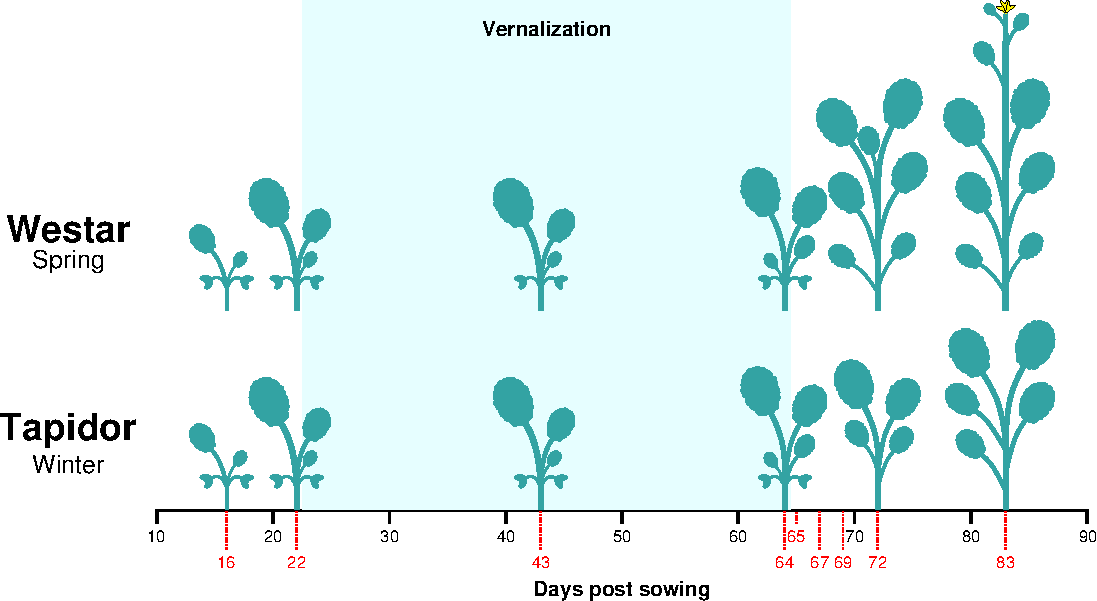
\includegraphics{figuredirectory/01_sampling_scheme.pdf}
\caption{\textbf{The sampling scheme for the transcriptome time series.}
Red numbers displayed below the bottom axis indicate the time points at
which the plants were sampled. The representations of the plants
indicate the approximate number of full leaves at those time
points.}\label{figure:201:samplingscheme}
\end{figure}

To capture transitions in gene expression relevant to flowering time
genes, the time points during development at which plant tissue was
sampled were carefully chosen. A schematic of the sampling scheme is
displayed in Figure \ref{figure:201:samplingscheme}. As with previous
studies investigating the vernalization
response\textsuperscript{139,225,233}, spring and winter varieties of
oilseed rape, called Westar and Tapidor respectively, were grown. Seeds
from both varieties were sown and plants grown under long day conditions
(16~hours of light) with controlled temperatures of 18~°C during the day
and 15 °C at night. The six week vernalization treatment involved
growing the plants in short day conditions (8~hours of light) at 5~°C.
Vernalization was necessary in order to accelerate the onset of
flowering for the winter variety, Tapidor. Although the spring variety
does not have a vernalization requirement, plants still exhibits a
vernalization response\textsuperscript{234}. To investigate this
facultative vernalization response of the spring variety, and to ensure
that data from the two varieties would be comparable, both Westar and
Tapidor plants were vernalized. To establish an appropriate
pre-vernalization baseline of gene expression, two time points were
sampled before the cold; one after two weeks of growth and another the
day before the plants were transferred into vernalization. A potential
confounding factor that the vernalization treatment introduces is the
change of both the temperature (15~-~18~°C to 5~°C) and the day length
(16~hours to 8~hours). Both changes in growth conditions were required
to make the vernalization treatment as physiologically accurate as
possible, as short days accompany the cold temperatures of winter.
However, transcriptional changes due to altered
photoperiod\textsuperscript{19,235} and
temperature\textsuperscript{236,237} have the potential to obscure the
response of genes to vernalization. To differentiate between expression
differences that result form these different flowering pathways, two
time points were sampled during the vernalization period; one halfway
through the treatment, after three weeks of cold, and another the day
before the treatment ended, after six weeks of cold. From results in
Arabidopsis, it is known that gene expression responds to changes in
photoperiod\textsuperscript{19,235} and ambient
temperature\textsuperscript{236,237} on the order of hours or days. The
vernalization response, however, changes gene expression over the course
of weeks\textsuperscript{28,238}. The mid-vernalization time point
allowed for these two transcriptional time scales to be resolved, while
the time point at the end of cold acts as a reference point for the
transcriptional changes expected to occur when the plants are taken out
of the cold. Sampling after the vernalization period was much more
frequent as rapid developmental changes were expected to occur after the
plants were returned to warmer temperatures and long day
conditions\textsuperscript{19,235}. Tissue was collected 1, 3, and 5
days post-vernalization to capture these expected shifts in the
transcriptome. To ensure that the developmental time period sampled for
each variety was comparable, the final two time points were sampled when
the plants had flower buds visible from above (BBCH stage
51\textsuperscript{239}). For the spring variety Westar this
developmental stage was reached 8 days post-vernalization, whereas for
Tapidor the final time point was sampled at 19 days post-vernalization.
Therefore, although the age of the spring and winter plants at the final
relevant time point (when the plants reached BBCH stage
51\textsuperscript{239}) differed, the developmental time period sampled
for the two varieties is very comparable.

\subsection{Reference genome sequence and gene
models}\label{section:spring:genomegenemodels}

In order to carry out RNA-Seq, short reads obtained from the sequencing
run have to aligned to a suitable reference
sequence\textsuperscript{240}. For \emph{B. napus}, three different
reference sequences are available. The set of \emph{B.napus} unigenes is
a community resource generated using expressed sequence tags from
\emph{B.napus}, \emph{B. oleracea}, and \emph{B.
rapa}\textsuperscript{241}. The aim with the unigene construction was to
resolve gene models of orthologous genes, such as homoeologous genes on
the A and C genome, and paralogous genes, which arose from the ancestral
genome triplication event in the \emph{Brassica}
lineage\textsuperscript{108,109}. The pan-transcriptome resource is in
many ways an updated version of the unigenes, utilizing published coding
DNA sequences (CDS) for \emph{B. napus}, \emph{B. oleracea}, and
\emph{B. rapa}\textsuperscript{242}. To generate the resource, CDS
models from the two diploid species were aligned to their respective
reference genomes. Gene models from the \emph{B. napus} reference
genome\textsuperscript{114} were then compared to the CDS models from
the diploid species, and any \emph{B. napus} gene models that did not
match any CDS model from the diploid species was added to the
pan-transcriptome\textsuperscript{242}. The final main reference
available was the \emph{B. napus} reference genome sequence itself,
sequenced from a European winter variety of oilseed rape called
Darmor-\emph{bzh}\textsuperscript{114}. While the unigenes and the
pan-transcriptome consist of tens of thousands of individual gene
models, the reference genome consists of genomic sequence arranged into
chromosomes. The advantage of such a reference is that gene models can
be viewed in a genomic context. In addition, the Tuxedo suite of tools
used to perform the quantification can more readily estimate total gene
expression, combining the expression from all isoforms of a gene, when a
genomic reference is used\textsuperscript{243}. To take advantage of
these benefits, the \emph{B. napus} genome sequence was used as the
reference sequence for the transcriptomic time series.

The Tuxedo suite of RNA-Seq tools is able to predict gene models from
RNA-Seq reads without prior knowledge of gene
models\textsuperscript{243}. This is possible due to TopHat aligning
reads in a splice-aware manner\textsuperscript{244}, allowing the intron
structure and the splice variants of genes to be discovered. Aligning
RNA-Seq reads obtained from the time series samples to the \emph{B.
napus} genome sequence using the Tuxedo suite resulted in two problems.
The first manifested in instances when neighbouring genes were oriented
on opposite strands with transcription occurring in the direction of the
other gene. Due to transcriptional read-through reads were obtained that
spanned the gap between the genes, causing the prediction algorithm to
combine the genes into a single gene model. These chimeric gene models
resulted in aberrant expression traces being generated. The other
problem arose as a result of genes that had undergone tandem
multiplication events, such that multiple copies of the gene were
located relatively close to each other in the genome. In this case,
reads that spanned across two exons would occasionally be aligned
partially to one gene in the tandem array and partially to another. This
lead to large gene models being predicted that spanned multiple genes in
the tandem array. The chimeric gene models created as a result of these
issues lead to additional reads mapping to these gene models, affecting
the expression level calculations.

To address these issues, predetermined gene models were used to quantify
gene expression. The Darmor-\emph{bzh} reference genome was published
with gene models predicted by \emph{ab initio} gene prediction, RNA-Seq
data, and mapping \emph{A. thaliana}, \emph{B. rapa}, \emph{B.
oleracea}, and \emph{Oryza sativa} protein sequences to the
genome\textsuperscript{114}. These different sources of data were
combined using the software GAZE\textsuperscript{245} and were weighted
differently based on the researchers confidence in the
data\textsuperscript{114}. However, weighting the data sources
introduces subjectivity to the gene models. To overcome this problem,
and to maximise the number of genes included in the transcriptomic time
series, an approach utilizing short reads obtained from the time series
samples was taken. The gene model prediction software
AUGUSTUS\textsuperscript{246} was used to combine evidence of gene
models from the RNA-Seq data directly into the Hidden Markov model based
prediction process. RNA-Seq reads from both tissues and varieties across
the entire time series was pooled and used to aid the prediction of
exon-inton boundaries. While the Darmor-\emph{bzh} gene models were also
directed by transcriptomic data, the short reads used were obtained from
roots, stems, leaves, and flower buds in low and high nitrogen
conditions\textsuperscript{114}. Potentially important floral genes that
are expressed during the period of development addressed in the current
study, therefore, may not have been represented in this dataset. By
using the short reads from the transcriptomic time series to aid the
generation of gene models, however, this problem is mitigated.

\begin{figure}[htbp]
\centering
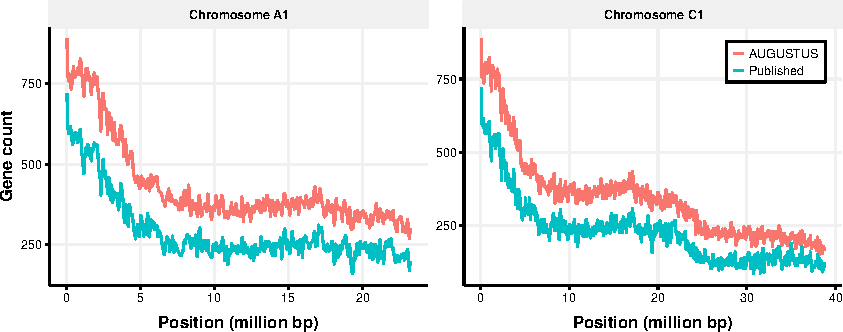
\includegraphics{figuredirectory/02_gene_position.pdf}
\caption{\textbf{Gene density is increased consistently across
chromosomes with the AUGUSTUS derived gene models relative to the
published gene models.} Gene count is calculated using a 100~kbp sliding
window across the chromosome. The patterns shown here are representative
of the patterns seen across all
chromosomes.}\label{figure:202:geneposition}
\end{figure}

\begin{figure}[htbp]
\centering
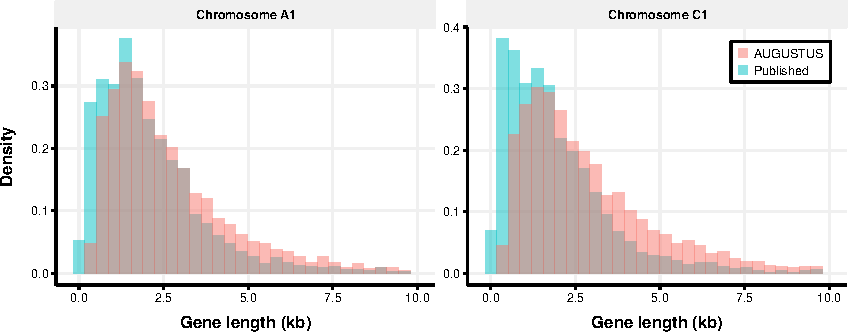
\includegraphics{figuredirectory/03_gene_length.pdf}
\caption{\textbf{AUGUSTUS derived gene models tend to be longer than
published gene models.} Gene length is calculated as the length of the
unprocessed mRNA transcript. The patterns shown here are representative
of the patterns seen across all chromosomes within a
genome.}\label{figure:203:genelength}
\end{figure}

The number of gene models obtained from AUGUSTUS\textsuperscript{246}
was 155,648, while the number of published gene models for the \emph{B.
napus} reference sequence is 101,040\textsuperscript{114}. To
investigate whether the gene models were distributed in the same way
across the genome, the density of genes across the genome was calculated
for both sets (Figure \ref{figure:202:geneposition}). The gene density
across the chromosomes is correlated between the two sets of gene models
(Figure \ref{figure:202:geneposition}). This result indicates that
similar proportions of genes are located in the same regions of the
genome in both gene model sets, despite the AUGUSTUS-derived models
exhibiting greater gene density. As gene density is greater for the
AUGUSTUS-derived models, one may expect that the length of the gene
models would be reduced due to models being split. In order to test
this, distributions of gene model lengths were calculated. The
AUGUSTUS-derived gene models are on average longer than the gene models
published with the Darmor-\emph{bzh} genome sequence (Figure
\ref{figure:203:genelength}). Taken together, these results suggest that
the AUGUSTUS-derived gene models better represent the genes present in
the \emph{B. napus} genome. This is due to the greater number of
AUGUSTUS-derived gene models relative to the published gene models, that
are not a consequence of gene models becoming split. Additionally, the
AUGUSTUS-derived gene models were able to resolve chimeric gene models
formed as a result of convergent transcription of genes and tandem
arrays of similar genes, discussed earlier. As a consequence of these
benefits relative to the published gene models, the AUGUSTUS derived
gene models were used to guide the RNA-Seq quantification process.

\subsection{Aligning reads and quantification of expression
levels}\label{section:spring:alignreadexplevel}

To quantify gene expression using RNA-Seq, short reads have to be
aligned to the chosen reference sequence to allow gene expression levels
to be estimated and normalized. There exist a number of different
methods for quantifying the expression level of genes using short read
data. A frequently used pipeline involves the Tuxedo suite of
tools\textsuperscript{243}. The pipeline consists of first aligning the
short reads using Bowtie\textsuperscript{247,248}, an alignment
algorithm which makes use of the Burrows-Wheeler transform of genomic
DNA sequence to allow for very efficient alignment. Bowtie is used by
another part of the Tuxedo suite called TopHat\textsuperscript{244}.
TopHat is a splice aware aligner; if a particular read does not align to
the reference sequence then the read is segmented and the individual
segments are aligned separately\textsuperscript{244}. In this way, reads
that span exon-exon boundaries can be detected, allowing different
splice isoforms to be detected and their expression quantified. Finally,
once the reads are aligned, Cufflinks is used to quantify gene
expression\textsuperscript{249}. This is done in a probabilistic manner
that takes into account both the error measured from different
biological replicates and the uncertainty in read mismapping. The latter
arises when reads align with equally high alignment scores in multiple
places in the genome. Instead of removing these reads from further
analysis, which has the potential to discard a lot of the sequencing
data collected, Cufflinks is able to incorporate this uncertainty into
the error associated with the expression
measurement\textsuperscript{249}. A more recent RNA-Seq analysis
pipeline involves the pseudoalignment of reads to a reference
transcriptome. Kallisto assigns reads to transcripts based on
\emph{k}-mer matching between the read and the
transcript\textsuperscript{250}. In order to take into account ambiguous
read mapping, Kallisto implements a bootstrap technique which resamples
the read assignments. This bootstrapping technique is made possible due
to the speed with which Kallisto runs and allows for the technical
variation within a sequencing run to be estimated\textsuperscript{250}.
While the speed and technical variation estimation of Kallisto are
advantages over the Tuxedo suite, the software requires transcript
sequences in order to be run. In the case of \emph{B. napus}, splice
isoforms are less well categorized than for other species, such as
Arabidopsis. Additionally, the downstream statistics pipeline for
Kallisto\textsuperscript{251} is designed to carry out differential
expression analysis using RNA-Seq data, rather than estimating
expression level taking into account technical and biological noise. Due
to these issues with Kallisto, and as the Tuxedo suite is a mature suite
previously used in other \emph{B. napus} RNA-Seq
studies\textsuperscript{252,253}, the latter was used to quantify gene
expression.

\begin{figure}[htbp]
\centering
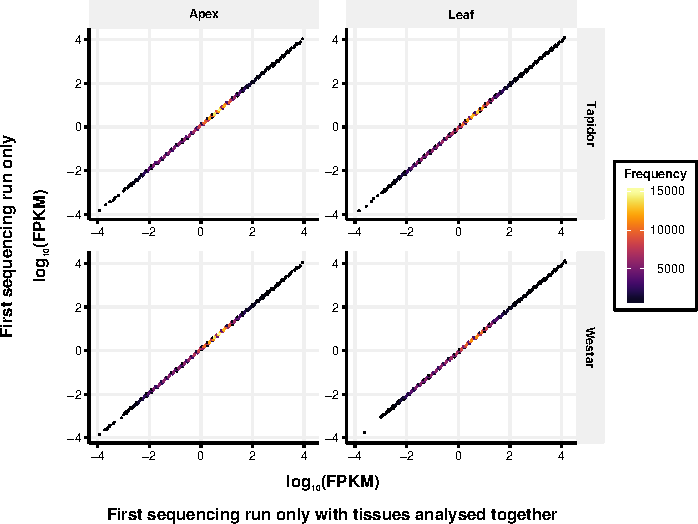
\includegraphics{figuredirectory/04_tissue_split_sequencing_fpkm.pdf}
\caption{\textbf{Quantifying gene expression for the apex and leaf
separately has little effect on FPKM values.} FPKM gene expression
values were calculated using the same quantification pipeline for both
the leaf and the apex samples from the first sequencing run combined
(x-axis) or separately (y-axis). These values were \(\log_{10}\)
transformed for clarity. That the points lie along the \(y = x\) line
indicates that both approaches result in similar FPKM values being
calculated. The data is displayed as a two dimensional histogram, where
the colour of the hexagonal unit indicates the number of data points
mapping to that part of the plot.}\label{figure:204:tissuesplitfpkm}
\end{figure}

\begin{figure}[htbp]
\centering
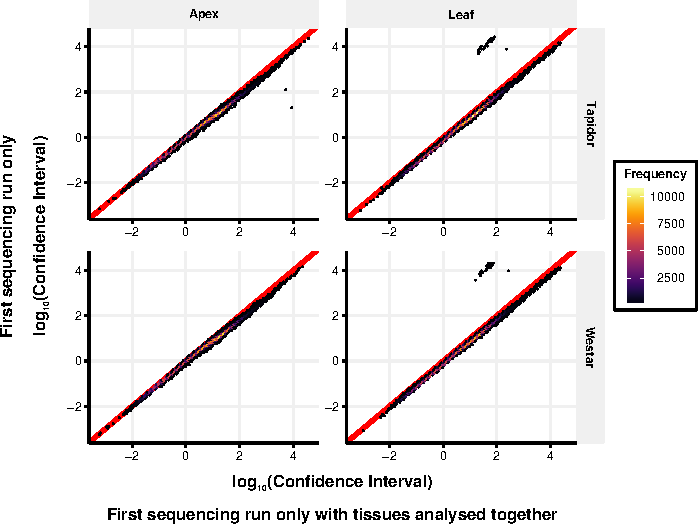
\includegraphics{figuredirectory/05_tissue_split_sequencing_confidence_interval.pdf}
\caption{\textbf{Calculating FPKM values for the apex and leaf
separately reduces the size of the confidence intervals.} 95~\%
confidence intervals were calculated using the same quantification
pipeline for both the leaf and the apex samples from the first
sequencing run combined (x-axis) or separately (y-axis). The ranges of
these intervals were \(\log_{10}\) transformed for clarity. That the
majority of points lie below the \(y = x\) line (red diagonal line)
indicates that calculating the confidence intervals separately for each
tissue reduces the uncertainty in the expression value measurement. The
data is displayed as a two dimensional histogram, where the colour of
the hexagonal unit indicates the number of data points mapping to that
part of the plot.}\label{figure:205:tissuesplitconf}
\end{figure}

To quantify gene expression for the the transcriptomic time series,
short reads were aligned to the \emph{B. napus} reference
genome\textsuperscript{114} using the AUGUSTUS-derived gene models
(discussed in Section \ref{section:spring:genomegenemodels}). Initially,
only short reads from a single sequencing run were available for each
sample, with an average of 67~million reads per sample obtained. Of
these total reads, 82~\% were mapped to the reference genome. The
confidence intervals calculated by Cufflinks using this sequencing data,
however, were too large to allow confident conclusions to be drawn from
the data. This was potentially due to Cufflinks not having information
from biological repeats to properly calculate confidence intervals, as
in the absence of multiple measurements for a sample Cufflinks treats
all samples as repeats of each other in order to parametrize the error
model used\textsuperscript{249}. To test if this was the case, gene
expression values were calculated separately for the two tissues. If the
large confidence intervals were indeed due to the lack of repeat
measurements, it was expected that only using samples of the same tissue
type to parameterize the error model would result in smaller confidence
intervals being calculated. Performing the analysis in this way lead to
a general reduction in the size of the confidence intervals calculated
for each expression level estimate (Figure
\ref{figure:205:tissuesplitconf}), while not affecting the expression
level estimations for genes (Figure \ref{figure:204:tissuesplitfpkm}).
This suggests that the initial size of the confidence intervals was
indeed because samples from different tissues, different varieties, and
different points in development were used to calculate the uncertainty.

\begin{figure}[htbp]
\centering
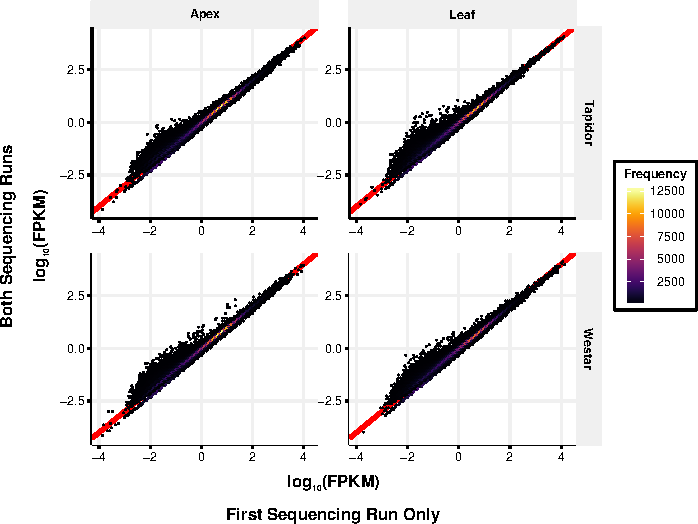
\includegraphics{figuredirectory/06_both_vs_first_sequencing_fpkm.pdf}
\caption{\textbf{Including data from a second sequencing run does not
affect the majority of estimated FPKM values.} FPKM gene expression
values were calculated using the same quantification pipeline for the
first sequencing run only (x-axis) or both sequencing runs combined
(y-axis). These values were \(\log_{10}\) transformed for clarity. That
the highest frequencies of points lie along the \(y = x\) line indicates
that both approaches result in similar FPKM values being calculated for
the majority of genes. The data is displayed as a two dimensional
histogram, where the colour of the hexagonal unit indicates the number
of data points mapping to that part of the
plot.}\label{figure:206:repsfpkm}
\end{figure}

\begin{figure}[htbp]
\centering
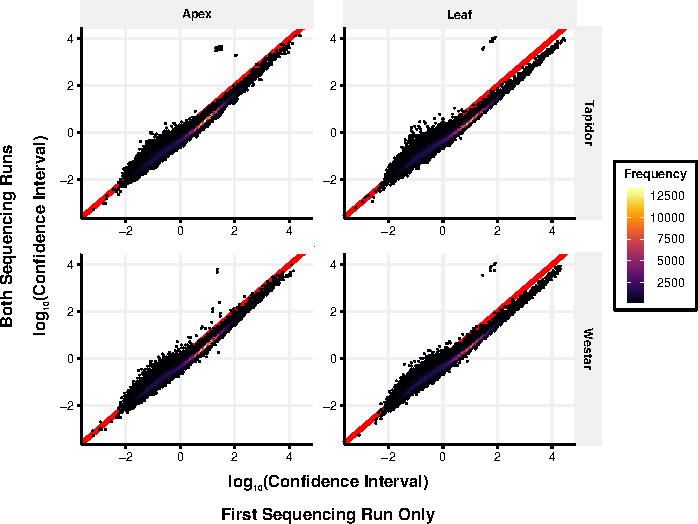
\includegraphics{figuredirectory/07_both_vs_first_sequencing_conf_interval.pdf}
\caption{\textbf{Including data from a second sequencing run causes a
reduction in the majority of estimated confidence interval sizes.} 95~\%
confidence intervals were calculated using the same quantification
pipeline for the first sequencing run only (x-axis) or both sequencing
runs combined (y-axis). The ranges of these intervals were \(\log_{10}\)
transformed for clarity. That the majority of points lie below the
\(y = x\) line (red diagonal line) indicates that calculating the
confidence intervals with reads from biological repeats reduces
uncertainty in the expression value measurements for the majority of
genes. The data is displayed as a two dimensional histogram, where the
colour of the hexagonal unit indicates the number of data points mapping
to that part of the plot.}\label{figure:207:repsconf}
\end{figure}

Although calculating expression values separately for each tissue
results in reduced confidence interval sizes relative to both tissues
combined, the intervals calculated were still large. To reduce the size
of the intervals further, a second pool of biological tissue was
sequenced. To ensure that the uncertainty in expression levels was
calculated accurately in both tissues across the entire time series,
samples selected to be in the second sequencing run were chosen to span
the entire time series. Samples from every time point were not required,
as the Cufflinks algorithm uses samples for which repeat measurements
are available to parameterize an error model, that is then applied to
samples that are lacking repeat measurements\textsuperscript{249}.
Additional pools of tissue from the apex and leaf, sampled at days 22,
43, 64, 67, and 72 of the time series, were sequenced with an average of
33~million reads per sample being obtained. As with the first sequencing
run, an average of 82~\% of reads mapped to the reference sequence.
Incorporating the repeat measurements resulted in a large reduction in
confidence interval sizes (Figure \ref{figure:207:repsconf}) while
having a comparatively small effect on expression levels for the
majority of measurements (Figure \ref{figure:206:repsfpkm}). Therefore,
the second sequencing run was able to provide enough additional data to
reduce the uncertainty in the gene expression level estimation to
acceptable levels for further work to be carried out.

\begin{figure}[htbp]
\centering
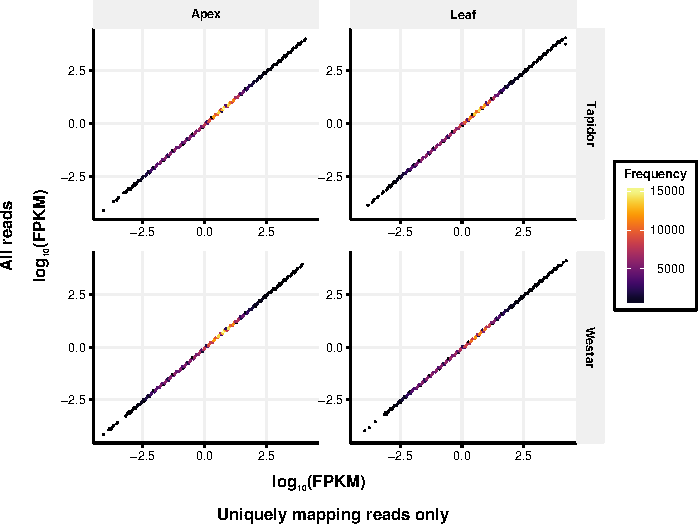
\includegraphics{figuredirectory/08_all_vs_unique_sequencing_fpkm.pdf}
\caption{\textbf{Reads aligning to multiple regions of the genome have
little effect on the estimated gene expression levels.} FPKM gene
expression values were calculated using the same quantification pipeline
for all reads (y-axis) or reads that only align to a single position in
the reference sequence (x-axis). These values were \(\log_{10}\)
transformed for clarity. That the points lie along the \(y = x\) line
indicates that both approaches result in similar FPKM values being
calculated for the majority of genes. The data is displayed as a two
dimensional histogram, where the colour of the hexagonal unit indicates
the number of data points mapping to that part of the
plot.}\label{figure:208:uniquefpkm}
\end{figure}

\begin{figure}[htbp]
\centering
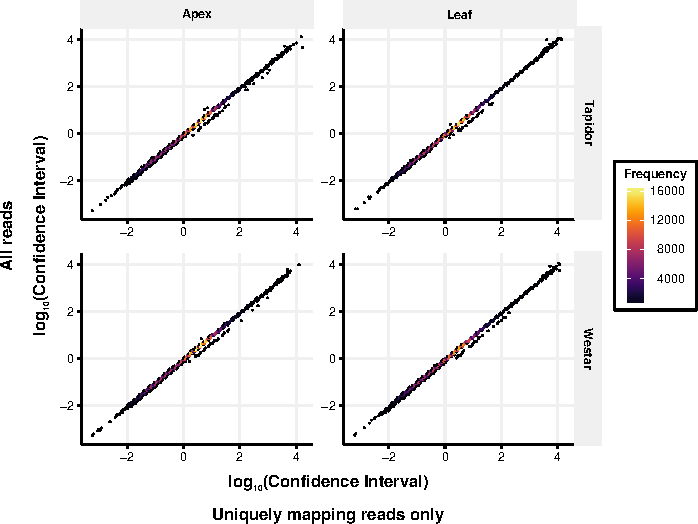
\includegraphics{figuredirectory/09_all_vs_unique_sequencing_conf_interval.pdf}
\caption{\textbf{Multiply mapping reads have little effect on the
estimated confidence interval range.} 95~\% confidence intervals were
calculated using the same quantification pipeline for all reads (y-axis)
or reads that only align to a single position in the reference sequence
(x-axis). The ranges of these intervals were \(\log_{10}\) transformed
for clarity. That the majority of points lie along the \(y = x\) line
indicates that both approaches result in similar confidence interval
ranges being calculated for the majority of genes. The data is displayed
as a two dimensional histogram, where the colour of the hexagonal unit
indicates the number of data points mapping to that part of the
plot.}\label{figure:209:uniqueconf}
\end{figure}

A potential issue with RNA-Seq are reads mapping equally likely to
multiple positions in the genome. To alleviate this problem, previous
studies investigating the differential expression of paralogous genes
have only used reads that map to single positions in the genome to
calculate expression levels\textsuperscript{254}. Cufflinks is able to
incorporate the uncertainty introduced by reads mapping to multiple
locations into the calculation of expression level
uncertainty\textsuperscript{249}. However, the high amount of duplicated
sequence in the \emph{B. napus} genome\textsuperscript{114} may result
in high uncertainty in the calculated expression levels. To investigate
whether this was the case, the effect on gene expression levels of reads
aligning to multiple positions in the genome was assessed. Of the reads
mapped to the genome, 14~\% were mapped to multiple positions in the
genome, with 0.3~\% in the first sequencing run and 0.4~\% in the second
sequencing run mapping to over twenty positions. To test if reads
mapping to multiple locations would affect the expression levels
calculated by Cufflinks, the expression level quantification was
repeated with these reads removed. Comparisons of FPKM values and
confidence interval ranges both reveal very little difference when reads
that map to multiple position in the genome are excluded from the
analysis (Figures \ref{figure:208:uniquefpkm} and
\ref{figure:209:uniqueconf}). This result demonstrates that reads
mapping to multiple positions in the genome are not adversely affecting
the calculation of expression levels and are therefore included in the
expression level quantification used throughout this study.

\subsection{Self-organizing map based clustering of expression
data}\label{section:spring:somexplanation}

\begin{figure}[htbp]
\centering
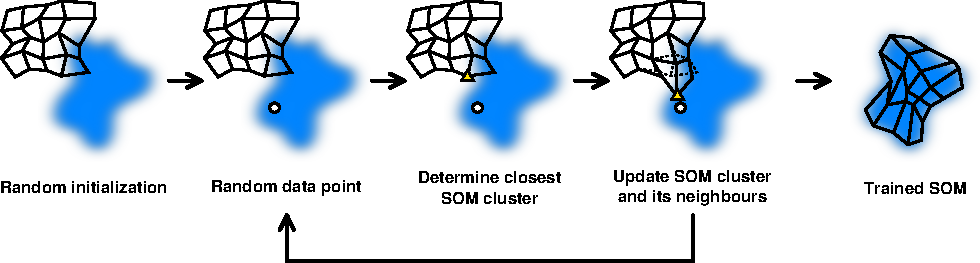
\includegraphics{figuredirectory/10b_som_explanation.pdf}
\caption{\textbf{Self-organizing maps (SOMs) are trained to represent
multidimensional datasets.} SOMs are randomly initiated. Clusters are
assigned neighbours based on their Euclidean distances from one another,
such that neighbouring clusters have a lower Euclidean distance between
them. During the training process, the SOM (black grid) is trained to
represent the dataset (blue shape). The training process begins by
selecting a random data point. The SOM cluster closest to that data
point (yellow triangle), determined by Euclidean distance, is translated
closer to the data point. At the same time, the neighbouring clusters
are also translated, although to a lesser extent. Another data point is
selected and the process repeats. The training process continues until
the SOM accurately represents the dataset. Image adapted from a diagram
by Mcld\textsuperscript{255}, distributed under a CC BY-SA 3.0
license}\label{figure:215:somexplanation}
\end{figure}

Having constructed the transcriptomic time series, validation was
conducted to determine if expected trends were observed in the dataset.
In order to assess trends in the data, gene expression profiles across
time were clustered using self-organizing maps (SOMs). SOMs adaptively
take into account the variation present in the data to ensure that the
dataset is properly represented. When used to cluster time series data,
each cluster represents an expression profile across time, with genes
exhibiting a similar expression profile assigned to that cluster. Due to
the process by which SOMs are trained to the dataset (Figure
\ref{figure:215:somexplanation}), neighbouring clusters will tend to
have similar expression profiles to each other. If particular parts of
the dataset are more dense in terms of the number of data points present
then the training process will explore that part of the dataset more,
leading to a higher density of clusters in that area. The ratio of grid
dimensions are set as the same ratio as the eigenvalues of the first two
principal components of the data, to maximise the variation captured by
the SOM (Section \ref{section:methods:somclustering}; Methods). These
properties lead to a clustering method that allows for the time series
data to be summarised and visualized in an intuitive manner. Only SOMs
generated using data from Westar are displayed here, with SOMs generated
using data from Tapidor discussed elsewhere in the thesis (Section
\ref{section:winter:som}).

\begin{figure}[htbp]
\centering
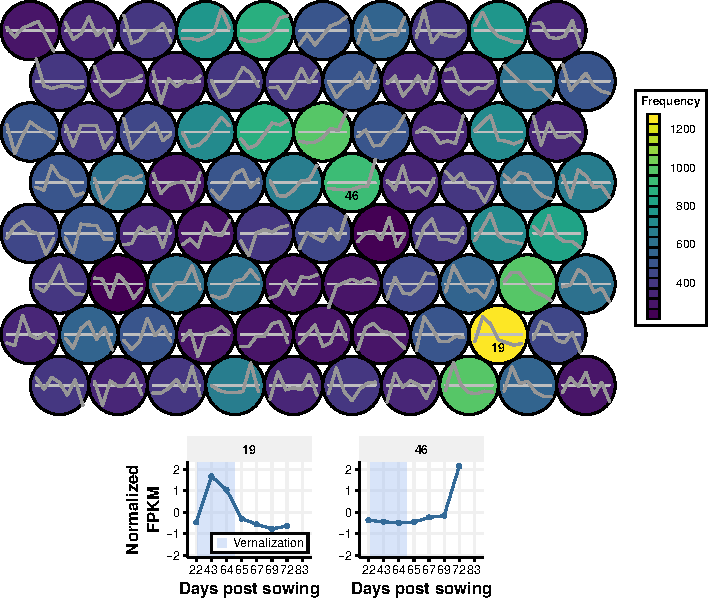
\includegraphics{figuredirectory/10c_a_w_som_count.pdf}
\caption{\textbf{SOM generated using the apex transcriptome time series
in Westar.} The size of the SOM was chosen such that it captured
\textasciitilde{}85\% of the global squared distance from the mean
(Section \ref{section:methods:somclustering}; Methods). The grey lines
within each SOM cluster indicate the normalized expression profile that
particular cluster represents. The SOM is toroidal, such that clusters
on the top and bottom rows are adjacent, as are clusters on the left and
right hand columns. The colour of the cluster represents the number of
genes mapped to that particular cluster. The graphs under the plot
correspond to clusters 19 and 46, that represent areas of the SOM with
high numbers of genes.}\label{figure:216:somaw}
\end{figure}

Within the SOM generated using the developmental transcriptome from the
apex (Figure \ref{figure:216:somaw}), there are two regions that have a
high number of genes mapped to them, represented by clusters 19 and 46.
The expression profile of cluster 19 is low at the start of the time
series, increases during the cold, and returning to pre-cold levels when
the plants are returned to growth in warmer conditions. The other region
of the map with a high number of genes mapped to it are the clusters
located towards the centre of the map and represented by cluster 46.
These clusters exhibit an expression pattern that remains largely
constant throughout the developmental time series, with an increase in
expression towards the final time point (Figure \ref{figure:216:somaw}).
These findings suggest that in the apex a large number of genes are
responding to the change in growth conditions in the vernalization
treatment, that is, short days and 5~°C temperatures. The large number
of genes that increase in expression at the final time point may be due
to flower buds being formed in the apex, which would require the
coordinated expression of many genes.

\begin{figure}[htbp]
\centering
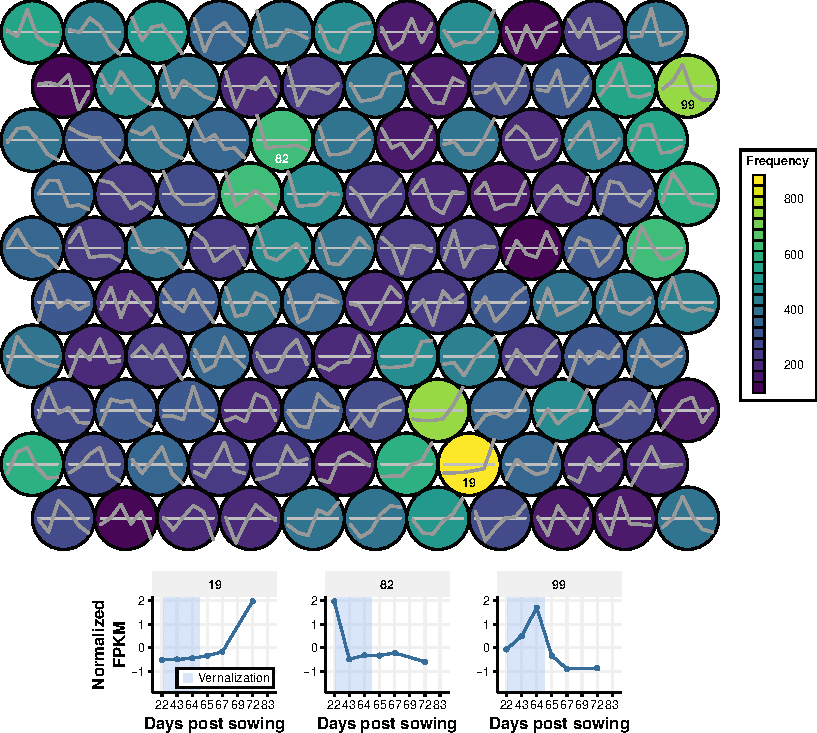
\includegraphics{figuredirectory/10d_l_w_som_count.pdf}
\caption{\textbf{SOM generated using the leaf transcriptome time series
in Westar.} The size of the SOM was chosen such that it captured
\textasciitilde{}85\% of the global squared distance from the mean
(Section \ref{section:methods:somclustering}; Methods). The grey lines
within each SOM cluster indicate the normalized expression profile that
particular cluster represents. The SOM is toroidal, such that clusters
on the top and bottom rows are adjacent, as are clusters on the left and
right hand columns. The colour of the cluster represents the number of
genes mapped to that particular cluster. The graphs under the plot
correspond to clusters 19, 82, and 99, that represent areas of the SOM
with high numbers of genes.}\label{figure:217:somlw}
\end{figure}

To determine whether trends similar to the apex would also be observed
in the leaf transcriptome, a SOM was generated for the leaf
transcriptome time series (Figure \ref{figure:217:somlw}). Three regions
of the leaf SOM exhibited high numbers of genes mapping to them;
represented by clusters 19, 82, and 99. Cluster 82 exhibits an
expression profile that is high initially, decreases during the
vernalization period, and remains lowly expressed when plants are
returned to warmer growth conditions. This suggests that a large number
of genes are becoming stably repressed during the cold period, which may
be due to a vernalization response or to effects resulting from the leaf
ageing during the time series. Clusters 19 and 99 exhibit similar
expression profiles as clusters 46 and 19 from the apex-derived SOM
(Figure \ref{figure:216:somaw}). This suggests that, as with the
apex-derived SOM, that a large number of genes are responding to growth
in the cold, short day conditions of the vernalization treatment.

SOMs have been used in previous investigations to cluster gene
expression traces\textsuperscript{256} and distil general trends from
time series expression data\textsuperscript{257}. To validate that the
transcriptome time series accurately captures important expression
profiles, SOMs were used to cluster data from the Westar leaf and apex
samples. Both of the SOMs for the leaf and apex reveal that a large
number of genes exhibited transcriptional responses to the change in
growth conditions that occur when the plants are grown in short days at
5~°C. Transcriptional changes occurring as a result of photoperiod and
temperature changes have been observed in
Arabidopsis\textsuperscript{19,235--237} and
ryegrass\textsuperscript{258}. That similar expression changes are
observed for the \emph{B. napus} transcriptome time series suggests that
key expression differences have indeed been captured by the experiment.
This result also highlights the importance of subjecting both the spring
and winter varieties to vernalization. As discussed in section
\ref{section:spring:experimentaldesign}, studying transcriptional
effects of vernalization requires differentiating between vernalization
responsive genes and genes that are affected by ambient temperature and
photoperiod changes\textsuperscript{225}. That a vernalization
responsive cluster and a cold treatment responsive cluster are
identified in the leaf SOM suggest this differentiation will be
possible. In addition, that a vernalization responsive cluster is
observed in the leaf in Westar, a spring variety, suggests that genes
controlling the vernalization response in Westar\textsuperscript{234}
and the vernalization requirement in Tapidor can be disentangled.
Finally, many genes increase in expression towards the final time point
in both tissues. This suggests that the transcriptional changes that
accompany the transition to floral growth have been captured by the
transcriptome time series.

\subsection{Gene ontology term
enrichment}\label{section:spring:gotermenrichment}

To further investigate general trends that the SOM clustering reveals,
enrichment analyses were carried out for gene ontology (GO) terms of
interest. Co-expressed genes may be part of the same developmental
pathway, or may be co-expressed as a consequence of the way the
experiment was designed\textsuperscript{259}. GO term enrichment is one
method of determining whether the observed clustering is biologically
meaningful. GO terms are a precise, fixed vocabulary for describing
where in an organism a gene acts, the molecular function of that gene,
and the biological process the gene is involved in. When GO gene
annotations are available for a particular organism, the proportion of
genes annotated with a particular GO term across the entire genome can
be determined. If a significantly higher proportion of genes within a
subset are annotated with a GO term than would be expected given the
across genome proportion, then that subset of genes is said to be
enriched for that GO term. To understand the expression dynamics of key
developmental pathways during the transcriptomic time series, GO term
enrichment was carried out using the clusters identified in the SOM
analysis (section \ref{section:spring:somexplanation}).

\begin{figure}[htbp]
\centering
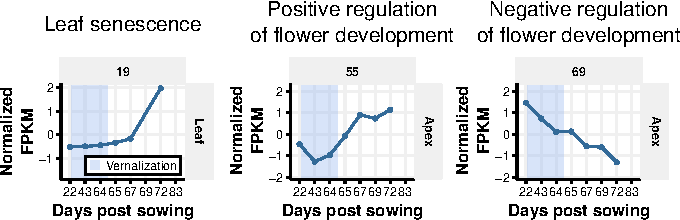
\includegraphics{figuredirectory/10e_go_term_enrichment_1.pdf}
\caption{\textbf{Normalized expression profiles for SOM clusters
enriched for leaf senescence and regulation of flower development.}
Normalized expression profiles for SOM clusters that are significantly
enriched for each GO term and that also contain the most \emph{B. napus}
genes annotated with that GO term are displayed. The expression patterns
of genes associated with ``leaf senescence'' in the leaf and regulation
of flower development in the apex are consistent with phenotypic
observations from those tissues.}\label{figure:219:go1som}
\end{figure}

To establish that GO term enrichment analysis would provide reliable
results, and to further validate the transcriptomic time series, the
enrichment of GO terms associated with phenotypic observations were
tested. During the time series, the first true leaf was sampled at every
time point (section \ref{section:spring:experimentaldesign}). As a
consequence, the leaf tissue sampled was older at later time points, and
some of the first true leaves had begun to visibly senesce by the final
time point. To test if this resulted in a change in the transcriptome in
the leaf, SOM clusters enriched for GO terms associated with ``leaf
senescence'' in the leaf data were determined. The most highly enriched
cluster identified in the leaf data for the term ``leaf senescence''
exhibits an expression pattern that gradually increases across the
entire time series, with a large increase in expression at the final
time point (Figure \ref{#figure:219:go1som}). This suggests that genes
associated with leaf senescence are co-expressed in \emph{B. napus}, a
finding also observed in the transcriptome of senescing Arabidopsis
leaves\textsuperscript{260}. The time points selected for the time
series were chosen to allow the progression of the floral transition to
be investigated (section \ref{section:spring:experimentaldesign}). An
expectation arising from this would be that GO terms relating to flower
development would exhibit expression changes across the time series. To
test whether this is the case, clusters enriched for the GO terms
``positive regulation of flower development'' and ``negative regulation
of flower development'' were identified in the apex-derived SOM. The
expression of genes annotated with the GO term ``positive regulation of
flower development'' increased during the time series, while genes
associated with the ``negative regulation of flower development''
decreased in expression across the time series in the apex (Figure
\ref{#figure:219:go1som}). These responses are consistent with
phenotypic observations that flower buds were visible from above (BBCH
stage 51\textsuperscript{239}) at the final time point in the series. An
additional observation for the expression traces of the cluster enriched
for genes associated with the positive regulation of flower development
is the slight decrease in expression during the vernalization treatment
(Figure \ref{#figure:219:go1som}). As will be discussed later in this
chapter when the behaviour of key floral integrators are investigated
(Section \ref{section:spring:ft}), this is likely a result of the short
day conditions the plants were grown in not being conducive to
flowering.

\begin{figure}[htbp]
\centering
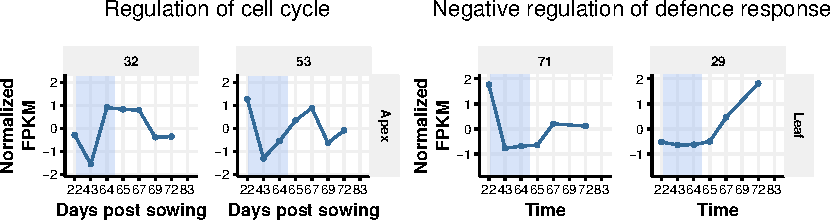
\includegraphics{figuredirectory/10f_go_term_enrichment_2.pdf}
\caption{\textbf{Normalized expression profiles for SOM clusters
enriched for regulation of cell cycle and defence response.} Normalized
expression profiles for the top two SOM clusters that are significantly
enriched for each GO term. The expression profiles of genes involved
with regulating the cell cycle in the apex decrease during the cold
treatment, suggesting that the cold temperature may involve a change in
the rate of cell division. The response of SOMs enriched for negative
regulation of defence response in the leaf suggest interplay between
defence responses, cold, and flowering.}\label{figure:220:go2som}
\end{figure}

Having established that clustering expression profiles from the
transcriptomic time series resulted in biologically relevant groupings
of genes, the enrichment of other GO terms was investigated. Controlling
the cell cycle is an integral aspect of growth that plants need to
tightly control. In terms of flowering, a sudden burst in the expression
of genes controlling the cell cycle was observed during the floral
transition in the shoot apical meristem of
Arabidopsis\textsuperscript{261}. This behaviour was hypothesised to be
a result of large scale meristem reorganization initiated by the floral
transition. In the apex-derived SOM, there are two main clusters
enriched for the GO term ``regulation of cell cycle''. Both clusters
exhibit high expression prior to the cold and a decrease in expression
during the cold (Figure \ref{figure:220:go2som}). Immediately after cold
the expression traces of these SOM clusters peak and before returning to
lower expression levels. The peak in expression after the vernalization
period is in line with the findings discussed for
Arabidopsis\textsuperscript{261}. The decrease in expression during the
vernalization period suggests that the cell cycle is responding to the
growth at lower temperatures. This result is in agreement with
observations from maize leafs, where the cell cycle duration increased
during growth in cold conditions and cell cycle related genes exhibited
differential expression\textsuperscript{262}.

The interactions between plant defence response, flowering and
temperature are beginning to be revealed in model
species\textsuperscript{237,263}. The energetic costs of growth and the
maintenance of an active immune response in the plant have to be
balanced to ensure robust development\textsuperscript{264--266}. In
Arabidopsis, mutants in a particular negative regulator of defence had
reduced seed production, indicating that negative regulation of defence
during the reproductive phase of plant development is
important\textsuperscript{267}. The \emph{PIF4} transcription factor in
Arabidopsis is not only important for the the thermal acceleration of
flowering\textsuperscript{237} but also for mediating the balance
between growth and pathogen immunity at different
temperatures\textsuperscript{263}. At low temperatures, immune responses
are upregulated and growth is inhibited, while at warmer temperatures
the immune response is downregulated and growth and flowering is
promoted. The expression profiles of SOM clusters enriched for genes
with the GO term ``negative regulation of defence response'' reflect
this (Figure \ref{figure:220:go2som}). Cluster 71 in the leaf-derived
SOM exhibits high expression initially, with a rapid reduction in
expression during the cold. Upon return to warmer growth conditions, the
expression increases. The other cluster enriched for genes involved with
down regulating plant defence responses is cluster 29. This cluster is
not affected by the cold treatment, but exhibits a steady increase in
expression after the treatment. Both of these observations point towards
the \emph{B. napus} defence response being modulated by temperature and
flowering in a similar manner to that observed in Arabidopsis.

\begin{figure}[htbp]
\centering
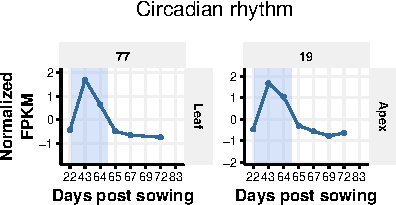
\includegraphics{figuredirectory/10g_go_term_enrichment_3.pdf}
\caption{\textbf{Normalized expression profiles for SOM clusters
enriched for genes associated with the circadian rhythm.} Normalized
expression profiles for the top two SOM clusters that are significantly
enriched for the GO term ``circadian rhythm'' in both tissues in Westar.
Both expression profiles increase during the cold treatment, suggesting
a response to the change in photoperiod or cold experienced during the
vernalization treatment.}\label{figure:221:go3som}
\end{figure}

To ensure the vernalization treatment was physiologically accurate,
plants were subjected to growth in short days at 5~°C. The spring
variety, Westar, was subjected to the vernalization treatment alongside
the winter variety, Tapidor, to allow for the transcriptomic effects of
photoperiod and ambient temperature changes to be differentiated from
the effects of vernalization (Section
\ref{section:spring:experimentaldesign}). To investigate the effects of
this treatment, SOM clusters enriched for the GO term ``circadian
rhythm'' were determined. The most highly enriched clusters in both the
leaf and the apex of Westar exhibit very similar expression traces
(Figure \ref{figure:221:go3som}). Both undergo increases in expression
during the cold treatment, with expression returning to pre-treatment
levels on the first day of growth post-treatment. This suggests that the
the altered photoperiod during the vernalization period results in
changes to the circadian clock, such as the clock becoming entrained to
the different light regime\textsuperscript{16}.

Although GO term enrichment is a relatively high level analysis that
does not investigate the gene level responses across the transcriptomic
time series, it is still a useful analysis for investigating the overall
behaviour of key developmental pathways. The results presented here
reveal a number of general trends that are in agreement with
observations in Arabidopsis. The response of the cell cycle and the
defence response genes to the period of cold the plants were subjected
to is in line with findings from Arabidopsis\textsuperscript{261,263}.
In the case of the behaviour of defence genes, the observation that the
response seems to be conserved between Arabidopsis and \emph{B. napus}
may have a future agronomic benefit. The expression response of genes
associated with the circadian rhythm confirms the requirement for two
time points to be sampled during the vernalization treatment. If a
single time point was sampled, the observed expression differences as a
result of the changing photoperiod would be indistinguishable from
effects due to a vernalization response.

\subsection{Protein domain
enrichment}\label{section:spring:proteinenrichment}

Proteins are modular in structure, composed of protein domains that are
often responsible for the molecular activity of the
protein\textsuperscript{268,269}. As a result, particular classes of
protein are associated with certain biological pathways or activities.
This is especially true with transcription factors, with different
transcription factor domains in Arabidopsis binding to distinct
recognition sequences\textsuperscript{270} and thus having distinct sets
of target genes. Investigating the expression of particular
transcription factor families across development can reveal the roles
they play in development\textsuperscript{271}. In order to take this
approach using transcriptomic time series, \emph{B. napus} gene models
were annotated with protein domains using previously published tools
(Section \ref{section:methods:proteinenrichment}; Methods). Two case
studies that illustrate the insights such an analysis facilitates are
MADS-box and AP2 domain containing proteins.

\begin{figure}[htbp]
\centering
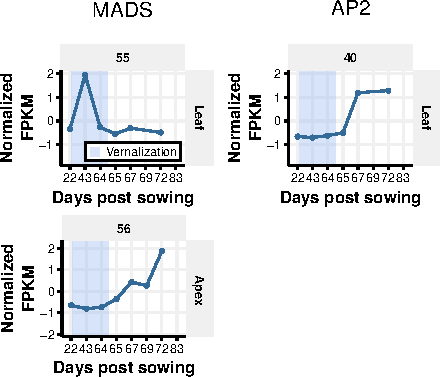
\includegraphics{figuredirectory/10h_protein_enrichment.pdf}
\caption{\textbf{Normalized expression profiles for SOM clusters
enriched for MADS and AP2 protein domains in the leaf and apex tissue of
Westar.} Normalized expression profiles for SOM clusters that are
significantly enriched for each protein domain and that also contain the
most \emph{B. napus} genes annotated with that protein domain are
displayed. The expression patterns of MADS-box containing genes exhibit
different patterns of expression in each tissue, suggesting that the
proteins play tissue-specific roles in development. The expression
profile of AP2 containing genes suggests that the proteins play a role
late in development in the leaf.}\label{figure:222:proteinsom}
\end{figure}

The MADS-box domain is a protein domain that is conserved across a
diverse array of species. Indeed, the MADS-box takes its name from the
\emph{MINICHROMOSOME MAINTENANCE 1} genes in yeast, the \emph{AGAMOUS}
gene in Arabidopsis, \emph{DEFICIENS} in \emph{Antirrhinum majus} and
serum response factor in humans\textsuperscript{272}. In Arabidopsis,
MADS-box containing genes have been found to control a wide range of
roles related to flowering\textsuperscript{273}. To determine the
regulation of this important family of proteins in \emph{B. napus}, the
clusters enriched for genes containing the domain were found (Section
\ref{section:methods:proteinenrichment}; Methods). In the leaf samples,
35 \emph{B. napus} genes with detectable MADS-box domains are expressed,
whereas 85 were expressed in the apex. The expression profiles for the
SOM clusters most highly enriched for MADS-box containing proteins are
quite different between the leaf and apex (Figure
\ref{figure:222:proteinsom}). The leaf cluster peaks in expression
during cold, with expression at the other time points, before and after
cold, being somewhat similar. The SOM cluster enriched in the apex
exhibits an expression trace that is lowly expressed before and during
cold but steadily increases after the cold to peak expression at the
final time point. To investigate why SOM clusters with such different
expression profiles were enriched for MADS-box containing genes, the
MADS-box containing genes within each cluster were scrutinised further.
The MADS-box containing genes mapping to cluster 55 in the leaf-derived
SOM correspond to genes involved with the control of flowering time such
as \emph{SVP}, \emph{FLC}, \emph{SOC1}, and
\emph{AGL24}\textsuperscript{28,79,81}. However, the genes mapping to
cluster 56 in the apex-derived SOM, however, include the meristem
identity controlling genes \emph{AP1} and \emph{FUL} and genes which are
involved with the ABCE model of flower morphology
control\textsuperscript{8,274}. All four of the gene classes of the
model are represented; A class (\emph{AP1}), B class (\emph{AP3} and
\emph{PI}), C class (\emph{AG}), and E class (\emph{SEP1}, \emph{SEP2},
and \emph{SEP4}). Therefore, the MADS-box containing genes within these
clusters represent different functional classes of MADS-box genes. The
upregulation of floral identity genes in the apex at the end of the time
series is consistent with the plants beginning to flower at the final
time points. The regulation of the MADS-box containing genes in the leaf
is likely related to the regulatory effects of the circadian rhythm
(Figure \ref{figure:221:go3som}), as the expression of \emph{SVP},
\emph{SOC1}, and \emph{AGL24} are all influenced by the photoperiod
pathway\textsuperscript{20,67,88,275}.

In addition to \emph{AP1}, another A class meristem identity gene
important for the specification of flower organ identity is the homeotic
gene \emph{APETALA2} (\emph{AP2})\textsuperscript{276}. The function of
the gene is dependent upon a 68 amino acid repeated motif called the AP2
domain\textsuperscript{277}. This domain has been found to be present in
a wide range of plant transcription factors that have been divided into
three familities; Ethylene Responsive Factors (ERF), AP2 and RAV
families\textsuperscript{278}. These proteins are involved in a wide
range of developmental processes as well as regulating metabolism and
stress responses\textsuperscript{278}. Investigating SOM clusters
enriched for genes containing the AP2 domain reveals cluster 40 in the
leaf-derived SOM as being highly enriched. The expression trace of
cluster 40 exhibits low expression initially and during cold with a
large increase in expression at the penultimate and final time points
(Figure \ref{figure:222:proteinsom}). This suggests that the AP2
containing genes contained in this cluster are involved with leaf
senescence (Figure \ref{figure:219:go1som}). This is consistent with the
observation that the majority of AP2 domain containing genes within
cluster 40 are members of the ERF family. Genes in this family are
frequently induced in response to stresses, and as their name suggests,
are responsive to plant hormones associated with stress; ethylene,
jasmonic acid and abscisic acid\textsuperscript{278}. The role ethylene
plays in leaf senescence\textsuperscript{279} also strengthens the
hypothesis that the AP2 domain containing genes within this cluster are
mediating this response.

\subsection{Conclusions}\label{conclusions}

To investigate regulatory changes during floral development in \emph{B.
napus}, a transcriptomic time series experiment was designed to dissect
the roles of different flowering time pathways. Sampling from both the
leaf and the apex allows a much richer view into flowering time
control\textsuperscript{13,15} as both tissues are involved with
different aspects of regulation. Developmentally similar tissues were
sampled from both a winter and a spring variety in order to generate the
time series. Comparing these two varieties will allow vernalization
responsive genes to be elucidated\textsuperscript{225}. This is
particularly important given the agronomic importance of the
vernalization response to the growth of \emph{Brassica}
crops\textsuperscript{123}. The reference sequence and downstream
expression analysis pipeline used to analyse the short read data were
chosen in order to make best use of the data. The final dataset is of
good quality, with uncertainty estimates that allow for the similarity
of expression traces across time to be quantified in a statistically
sound manner.

Initial analysis of the transcriptomic time series was focused on
validating the responses of key developmental pathways. In order to
carry this out, SOMs were generated to cluster the expression profiles
across time. Two main expression responses were observed in both the
apex and leaf of the spring variety; a response to the changing growth
conditions of the vernalization treatment and an increase in expression
towards the end of the time series. Analysis of GO terms suggest that
the transcriptomic response to the vernalization treatment is in part a
response to the change in photoperiod, as would be expected given
results from Arabidopsis\textsuperscript{16}. As the photoperiod pathway
is a key floral pathway\textsuperscript{15,17,18}, other expression
profiles for flowering time genes during the time series should be
viewed with this response in mind. The large number of genes in both
tissues increasing in expression towards the end of the time series seem
to be the result of different developmental pathways. In the leaf, the
response of genes annotated with the GO term ``leaf senescence'' (Figure
\ref{figure:219:go1som}) and genes containing the AP2 protein domain
(Figure \ref{figure:222:proteinsom}) suggest that leaf ageing is a
strong influence on transcriptional responses in the tissue. In
contrast, the increase at the final time point in the apex seems to be
linked to floral development (Figures \ref{figure:219:go1som} and
\ref{figure:222:proteinsom}). Interestingly, MADS-box containing genes
known to repress each other are co-expressed in the SOM cluster enriched
for MADS-box containing genes (Figure \ref{figure:222:proteinsom}). For
example, \emph{AG} represses the expression of \emph{AP1} in the inner
two whorls of the flower\textsuperscript{52}, while \emph{AP2} limits
the expression domain of \emph{AG}\textsuperscript{280}. This
co-expression illustrates that the dissection of the apex is not able to
resolve the distinct expression zones in the apex\textsuperscript{13}.
The alignment of key developmental pathways with phenotypic observations
and expectations from model species demonstrates that the transcriptomic
time series is able to capture biologically relevant changes in
expression.

\section{Regulatory divergence at the whole genome
scale}\label{section:spring:genomedivergence}

The effects of polyploidy on gene expression are varied and seemingly
influenced by the species and the time since
hybridization\textsuperscript{281}. Immediately following hybridization,
large transcriptional changes are observed in polyploids{[}282;
flagel\_evolutionary\_2010{]}. In synthetic Arabidopsis allopolyploids,
Wang et al. (2006)\textsuperscript{283} observed different contributions
to the transcriptome from the different constituent genomes, consistent
with extensive gene silencing following polyploidy\textsuperscript{284}.
These results from Arabidopsis allopolyploids demonstrate a major way in
which gene expression can vary after polyploidy: genome dominance.
Genome dominance is observed when the combined gene expression of gene
pairs from the two constituent genomes of a polyploid are consistently
biased towards a particular genome\textsuperscript{285,286}. These
expression inequalities may influence the evolution of the polyploid,
with results in maize revealing that gene loss favours copies that
contribute less to overall expression\textsuperscript{287}. In cotton
(\emph{Gossypium raimondii}) 99.4~\% of \textasciitilde{}2,000 gene
pairs exhibited biased expression in at least one of the three tissues
tested\textsuperscript{254}. Interestingly, this bias was found to be
tissue specific, suggesting that homologous genes may diverge to become
tissue specific over evolutionary time\textsuperscript{254,285}.

In order to investigate global differences in expression between the
genomes of \emph{B.~napus}, the expression of genes on the separate
genomes were compared using the transcriptomic time series. The genome
of origin seems to influence the expression of genes in the
\emph{B.~napus} genome, with different patterns of expression bias
observed at the genome-wide level relative to homoeologue level
comparisons. Investigating the retention of genes reveals that flowering
time genes have been retained in the \emph{B.~napus} genome, and that
this is also observed among the subset of expressed genes. This suggests
that the retained gene copies may be functional. Determining expression
pattern divergence among flowering time gene homologues in
\emph{B.~napus} reveals that the majority exhibit regulatory divergence.
This suggests that regulatory divergence has contributed to the
retention of flowering time genes in \emph{B.~napus}, although this has
occurred alongside potential gene dosage effects.

\subsection{Genome level expression differences between the A and C
genomes}\label{section:spring:genomelevel}

\begin{figure}[htbp]
\centering
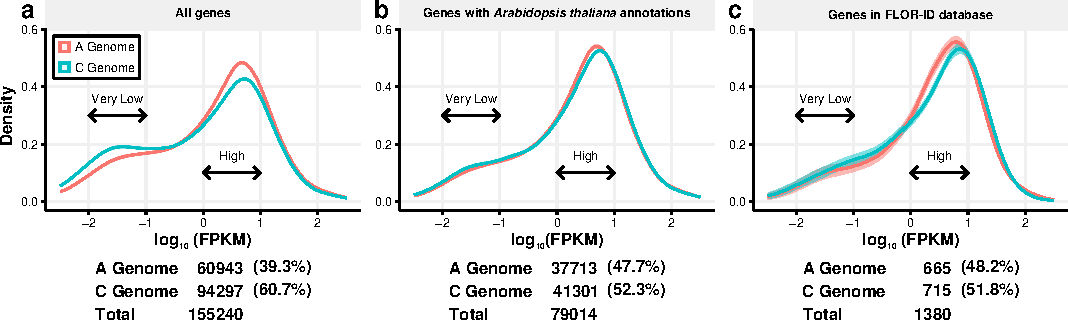
\includegraphics{figuredirectory/10i_genome_level.pdf}
\caption{\textbf{The \emph{B.~napus} A and C genomes show different
overall patterns of gene expression.} Density plots of transformed
expression levels (\(\log_{10}(FPKM)\)) calculated using different
subsets of genes. The expression data was sampled 1000 times using a
Gaussian error model. The density plot of \(\log_{10}(FPKM)\) values was
calculated for each sample. The mean density and the 95~\% confidence
interval estimated using the 1000 samples is displayed. Tabulated below
each density plot are the number of Brassica napus genes used to
calculate the density plot, separated by their genome of origin. The
data used to generate the density plots consisted of expression data
from: \textbf{a} all annotated \emph{B.~napus} genes, \textbf{b}
\emph{B.~napus} genes that show sequence conservation to an annotated
Arabidopsis gene, and \textbf{c} \emph{B.~napus} genes that show
sequence conservation to an annotated Arabidopsis gene that is present
in the FLOR-ID database\textsuperscript{288}. These plots are generated
using apex expression data from the time point taken at day 22, but are
representative of the density plots obtained for all time points across
both tissue types sampled (Figure \ref{appendixa:sampledensity};
Appendix A).}\label{figure:210:genomeexp}
\end{figure}

Previous studies of gene expression in polyploid species have generally
focussed on comparing the expression of genes on different genomes to
determine whether expression was
biased\textsuperscript{282,283,289--291}. To determine whether such a
bias was observed in the expression data from the transcriptomic time
series, density plots of the gene expression data for each of the two
genomes was generated (Figure \ref{figure:210:genomeexp}). Different
regions of the density curves will hereafter be referred to as very low
(below -1), low (between -1 and 0), high (between 0 and 1), and very
high (above 1), relating to the expression of genes within those
regions. The A genome has a greater proportion of genes in the high
expression region relative to the C genome (Figure
\ref{figure:210:genomeexp}a). Conversely, for genes in the very low
expression region, the opposite trend is observed (Figure
\ref{figure:210:genomeexp}a). Similar patterns are observed when only
\emph{B.~napus} genes exhibiting sequence conservation to an annotated
Arabidopsis gene are considered (Figure \ref{figure:210:genomeexp}b) and
when \emph{B.~napus} flowering time homologues are considered (Figure
\ref{figure:210:genomeexp}c). However the differences between the
density plots are less apparent when these subsets are taken.
Interestingly, the proportions of genes represented from each genome
change when these subsets of genes are taken. When no subset is taken,
approximately 40~\% of \emph{B.~napus} gene models are located on the A
genome. When subsets are taken, however, the percentage of genes on the
A genome is 48~\% in both cases (Figure \ref{figure:210:genomeexp}).
This difference reveals that there are more genes on the C genome that
do not show sequence conservation to an Arabidopsis gene.

\begin{table}[htp]
\caption{\textbf{Number of genes expressed two-fold higher than their homoeologue for all homoeologue pairs.} Homoeologue pairs were determined and filtered at each time point for those which both had expression levels above 2\ FPKM. The number and percentage of these genes expressed two-fold higher than their homoeologue is indicated. The geometric mean of the fold difference of the C genome gene relative to the A genome homoeologue for all homoeologue pairs is 1.12 in the apex and 1.11 in the leaf.}
\begin{center}
\resizebox{\textwidth}{!}{%
\begin{tabular}{ccccccc}
\toprule
\multirow{3}{*}{\parbox{1.5cm}{\centering Days post sowing}} &
\multicolumn{3}{c}{Apex} &
\multicolumn{3}{c}{Leaf} \\
\cmidrule(lr){2-4}\cmidrule(lr){5-7}
 & \parbox{2cm}{\centering Both expressed} &
 \parbox{2cm}{\centering A genome two-fold higher} &
 \parbox{2cm}{\centering C genome two-fold higher} &
 \parbox{2cm}{\centering Both expressed} &
 \parbox{2cm}{\centering A genome two-fold higher} &
 \parbox{2cm}{\centering C genome two-fold higher} \\
\midrule
22 & 7313 & 596 (8.1\ \%) & 1113 (15.2\ \%) & 6294 & 620 (9.9\ \%)  & 1066 (16.9\ \%) \\
43 & 7389 & 597 (8.1\ \%) & 1132 (15.3\ \%) & 6176 & 626 (10.1\ \%) & 1133 (18.3\ \%) \\
64 & 7325 & 602 (8.2\ \%) & 1085 (14.8\ \%) & 6307 & 597 (9.5\ \%)  & 1021 (16.2\ \%) \\
65 & 7243 & 609 (8.4\ \%) & 1120 (15.5\ \%) & 6182 & 601 (9.7\ \%)  & 993 (16.1\ \%)  \\
67 & 7299 & 601 (8.2\ \%) & 1135 (15.6\ \%) & 6257 & 603 (9.6\ \%)  & 1046 (16.7\ \%) \\
69 & 7342 & 594 (8.1\ \%) & 1130 (15.4\ \%) &   -  &      -       &      -        \\
72 & 7449 & 612 (8.2\ \%) & 1119 (15.0\ \%) & 6237 & 601 (9.6\ \%)  & 1054 (16.9\ \%) \\
\bottomrule
\end{tabular}%
}
\end{center}
\label{spring:table201:homoeologues}
\end{table}\begin{table}[htp]
\caption{\textbf{Number of genes expressed two-fold higher than their homoeologue for all flowering time gene homoeologue pairs.}
As for Table \ref{spring:table201:homoeologues}, calculated using homoeologue pairs that showed sequence similarity to Arabidopsis flowering time genes from the FLOR-ID database[TODO]. The geometric mean of the fold difference of the C genome gene relative to the A genome homoeologue for all flowering time homoeologue pairs is 1.10 in the apex and 1.04 in the leaf.}
\begin{center}
\resizebox{\textwidth}{!}{%
\begin{tabular}{ccccccc}
\toprule
\multirow{3}{*}{\parbox{1.5cm}{\centering Days Post Sowing}} &
\multicolumn{3}{c}{Apex} &
\multicolumn{3}{c}{Leaf} \\
\cmidrule(lr){2-4}\cmidrule(lr){5-7}
 & \parbox{2cm}{\centering Both Expressed} &
 \parbox{2cm}{\centering A Genome two-fold higher} &
 \parbox{2cm}{\centering C Genome two-fold higher} &
 \parbox{2cm}{\centering Both Expressed} &
 \parbox{2cm}{\centering A Genome two-fold higher} &
 \parbox{2cm}{\centering C Genome two-fold higher} \\
\midrule
22 & 136 & 11  (8.1\ \%) & 19 (14.0\ \%) & 109 &  8 (7.3\ \%)  & 14 (12.8\ \%) \\
43 & 149 & 15 (10.1\ \%) & 24 (16.1\ \%) & 118 & 12 (10.2\ \%) & 16 (13.6\ \%) \\
64 & 147 & 12  (8.2\ \%) & 20 (13.6\ \%) & 114 & 11 (9.6\ \%)  & 13 (11.4\ \%) \\
65 & 145 & 13  (9.0\ \%) & 25 (17.2\ \%) & 108 & 10 (9.3\ \%)  & 16 (14.8\ \%) \\
67 & 138 & 14 (10.1\ \%) & 19 (13.8\ \%) & 112 &  7 (6.3\ \%)  & 12 (10.7\ \%) \\
69 & 139 & 11  (7.9\ \%) & 18 (12.9\ \%) &  -  &     -      &     -      \\
72 & 142 & 15 (10.6\ \%) & 21 (14.8\ \%) & 112 &  5 (4.5\ \%)  & 14 (12.5\ \%) \\
\bottomrule
\end{tabular}%
}
\end{center}
\label{spring:table202:floweringhomoeologues}
\end{table}

To compare expression changes between the A and C genomes at the gene
level, as has been done previously\textsuperscript{292}, a list of
homoeologues was generated by genomic synteny and sequence similarly,
following a published method\textsuperscript{114}. Pairs of homoeologues
were classified as exhibiting biased expression in the direction of a
particular genome if the gene on that genome had an FPKM expression
value at least two-fold higher than the gene on the other genome. Biased
expression occurs in the direction of both genomes, although there is a
clear preference, with approximately double the number of pairs showing
biased expression towards the C genome rather than the A genome (16.9~\%
towards the C genome relative to 9.7~\% towards the A genome in the
apex, and 15.2~\% compared to 8.2~\% in the leaf; Table
\ref{spring:table201:homoeologues}). This pattern is consistent with the
findings of Chalhoub et al. (2014)\textsuperscript{114}, and is
maintained across the entire time series and for both tissue types
sampled (Figure \ref{appendixa:sampledensity}; Appendix A). Although
more pairs of homoeologues show biased expression towards the C genome
that the A genome, the pairs biased toward the A genome may exhibit
larger fold differences. If the overall expression of homoeologues was
balanced between the two genomes in this way, the geometric mean of the
fold differences of the C genome genes relative to their A genome
homoeologues should equal unity. Calculating the geometric mean reveals
a value above 1 (Table \ref{spring:table201:homoeologues}) demonstrating
that, on average, expression is biased towards the C genome. When pairs
of homoeologue identified as \emph{B.~napus} flowering time genes are
tested in the same way, patterns are largely maintained although are
less consistent across the time series due to fewer genes being
considered (Table \ref{spring:table202:floweringhomoeologues}).

Investigating expression differences between the two genomes of
\emph{B.~napus} reveals expression bias, although the direction of the
bias depends on the scale at which it is considered. The results from
the genome level analysis suggest an expression bias towards the A
genome, while the homoeologue level results suggest bias towards the C
genome. This discrepancy may be due to genes with low expression levels
tending to lack homoeologue pair information (Figure
\ref{appendixa:homoeologuedensity}; Appendix A). It is interesting that
the bias towards the A genome observed at the genome scale is less
apparent when \emph{B.~napus} genes lacking sequence conservation an
Arabidopsis gene are removed. This potentially indicates a higher
proportion of silenced or pseudogenes on the C genome, consistent with
the higher DNA methylation levels and transposon density observed in the
C genome\textsuperscript{114}.

\subsection{Tissue specific expression is biased towards the
apex}\label{section:spring:tissuespecfic}

\begin{figure}[htbp]
\centering
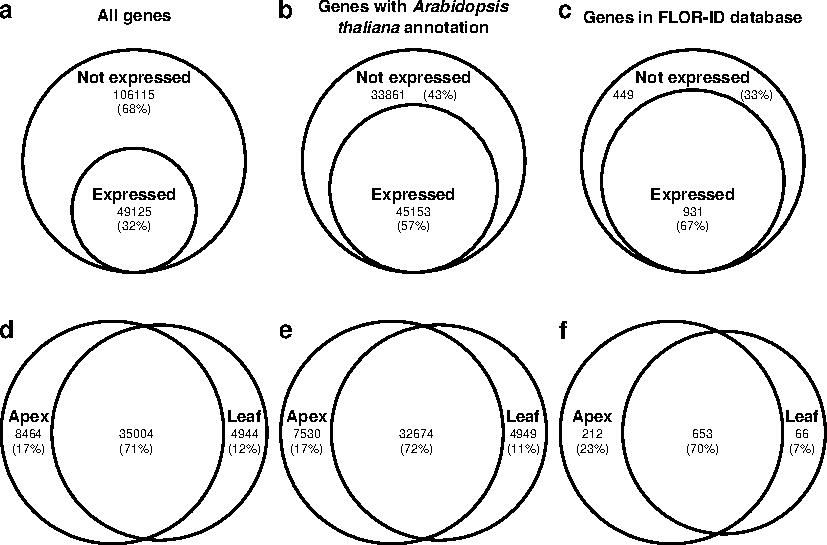
\includegraphics{figuredirectory/11_expressed_gene_venn_diagram.pdf}
\caption{\textbf{The majority of annotated \emph{B.~napus} genes are not
expressed.} \textbf{a-c} Euler diagrams indicating the percentage of
genes that are expressed and those that are not in the developmental
time series. A gene was regarded as expressed if the expression level of
the gene exceeded 2.0 FPKM at at least one time point in either the leaf
or apex sample. \textbf{d-f} Venn diagrams indicating the number of
expressed genes showing tissue specific expression. \textbf{a and d} All
annotated \emph{B.~napus} genes; \textbf{b and e} Only \emph{B.~napus}
genes with an identified Arabidopsis homologue are considered; \textbf{c
and f} Only \emph{B.~napus} genes with an identified Arabidopsis
homologue that is in the FLOR-ID database\textsuperscript{288} are
considered.}\label{figure:211:venn}
\end{figure}

The genome level analysis uncovered expression biased expression between
the two genomes of \emph{B.~napus}. In order to investigate other forms
of expression bias in the data, the number of genes exhibiting tissue
specific expression during the transcriptome time series was assessed.
Genes were classified as expressed during the time series if the
expression of the gene exceeded 2.0~FPKM at at least one time point. By
this definition, 32~\% of annotated \emph{B.~napus} genes were
classified as expressed in the developmental time series (Figure
\ref{figure:211:venn}). This percentage increases to 57~\% and 67~\%
when only \emph{B.~napus} genes with Arabidopsis homologues or
\emph{B.~napus} flowering time genes were considered, respectively. The
finding that there are many lowly expressed \emph{B.~napus} genes that
lack an Arabidopsis homologue is consistent with the results presented
in section \ref{section:spring:genomelevel}. Potentially these lowly
expressed genes that lack sequence similarity to annotated Arabidopsis
genes are pseudogenes. Taking all \emph{B.~napus} genes, regardless of
whether they have an Arabidopsis homologue or not, reveals that of the
49,125 genes that are expressed during the developmental time series,
17~\% are expressed specifically in the apex and 12~\% are expressed
specifically in the leaf, with the remaining 71~\% of genes expressed in
both tissues (Figure \ref{figure:211:venn}d). These percentages remain
largely unchanged when \emph{B.~napus} genes lacking an Arabidopsis
homologue are removed (Figure \ref{figure:211:venn}e). For flowering
time genes the percentage of genes exhibiting tissue specific expression
shifts towards the apex. Of the 931 expressed \emph{B.~napus} flowering
time genes, 23~\% are specifically expressed in the apex and 7~\% of
genes are leaf specific (Figure \ref{figure:211:venn}). This analysis
reveals that the majority of genes do not exhibit tissue specific
expression. Of those that do, there are more genes specifically
expressed in the apex than the leaf, perhaps as a result of the apex
undergoing a greater developmental change during the time series than
the leaf. The percentage of genes exhibiting tissue specific expression
changes depending on the subset of genes taken, with \emph{B.~napus}
flowering time genes having 76~\% of tissue-specific genes expressed in
the apex compared to 63~\% for all genes. This supports the hypothesis
that it is the apex transitioning to vegetative to floral growth that
results in more genes having an apex specific expression domain.

\subsection{\texorpdfstring{Multiple copies of flowering time genes have
been retained in the \emph{B.~napus}
genome}{Multiple copies of flowering time genes have been retained in the B.~napus genome}}\label{section:spring:floweringretained}

\begin{figure}[htbp]
\centering
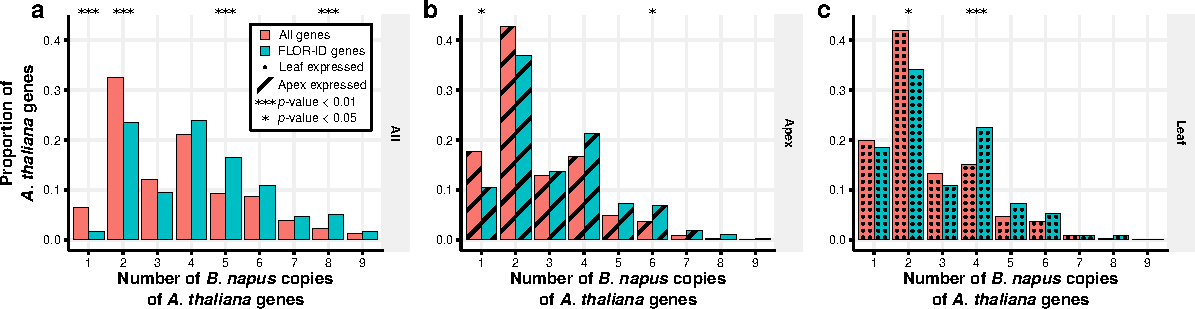
\includegraphics{figuredirectory/12_retention_distributions.pdf}
\caption{\textbf{Multiple \emph{B.~napus} flowering time gene homologues
are expressed during the floral transition.} This plot shows the
proportions of Arabidopsis genes that have particular numbers of
homologues identified and expressed in \emph{B.~napus}. \emph{B.~napus}
genes were considered to be expressed if their maximal expression level
within a tissue across the time series was above 2.0~FPKM. False
discovery corrected \emph{p-values} were computed by taking 1000 samples
of genes from the All distribution. The mean and standard deviation of
these samples were used to perform a two-tailed test of observing a
proportion as extreme as the FLOR-ID value. \textbf{a} \emph{B.~napus}
genes that show sequence conservation to an annotated Arabidopsis gene.
\textbf{b} \emph{B.~napus} genes expressed in the apex tissue that show
sequence conservation to an annotated Arabidopsis gene. \textbf{c}
\emph{B.~napus} genes expressed in the leaf tissue that show sequence
conservation to an annotated Arabidopsis
gene.}\label{figure:212:retentiondistribution}
\end{figure}

Genes that have undergone duplication in the genome and have been
subsequently retained are either under a selective pressure to be
maintained or have not yet been lost due to genetic
drift\textsuperscript{208,211}. To investigate whether the flowering
time genes have been retained in the genome, distributions of
Arabidopsis gene copies were calculated. These distributions are derived
by assigning \emph{B.~napus} genes to the Arabidopsis gene with the
highest sequence similarity, then counting the number of copies of each
Arabidopsis gene in the \emph{B.~napus} genome. This was done separately
for all Arabidopsis genes and for the subset that have been identified
as genes involved with flowering\textsuperscript{288} and the
distributions compared. Significant differences between the
distributions are observed at low copy numbers, with there being fewer
Arabidopsis flowering time genes with one or two copies in
\emph{B.~napus} than expected given the distribution for all genes
(Figure \ref{figure:212:retentiondistribution}a). At higher copy
numbers, a significantly higher proportion of Arabidopsis flowering time
genes have five and eight \emph{B.~napus} copies relative to the
distribution for all genes. To determine if this pattern was also true
for expressed \emph{B.~napus} genes, similar distributions were
generated for expressed genes in the apex (Figure
\ref{figure:212:retentiondistribution}b) and leaf (Figure
\ref{figure:212:retentiondistribution}c). These distributions also
reveal a shift towards the expression of a higher number of flowering
time gene copies relative to the whole genome. In general, flowering
time genes tend to have a lower proportion of genes expressed at low
copy numbers (three and below) and higher proportions at higher copy
numbers. This is indicative of the flowering time genes in
\emph{B.~napus} having been retained in the genome following the genome
multiplication events that have occurred throughout the evolutionary
history of \emph{B.~napus}. In addition, that these patterns are also
observed for expressed genes suggests that the retained flowering time
genes are functional.

\subsection{Expression divergence in the number of expressed copies of
annotated genes}\label{section:spring:expressedvsannotated}

\begin{figure}[htbp]
\centering
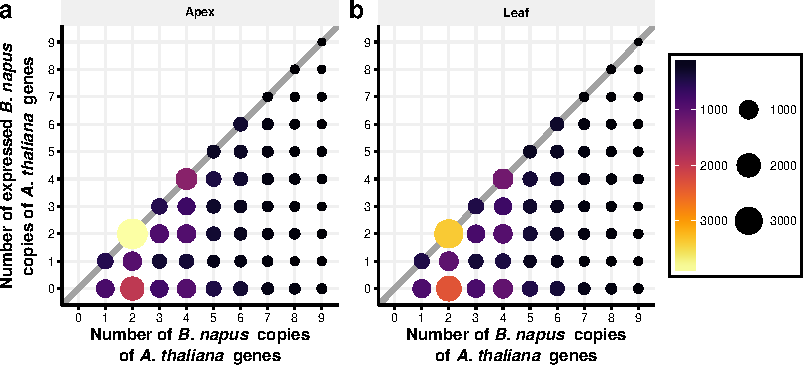
\includegraphics{figuredirectory/13_all_vs_exp_all_genes.pdf}
\caption{\textbf{Not all copies of genes are expressed in
\emph{B.~napus}.} Copies of Arabidopsis genes were identified in the
\emph{B.~napus} gene models through sequence similarity. These copies
were regarded as expressed if their maximum expression level during the
entire time series exceeded 2.0 FPKM. The size and colour of the cirlces
indicates the number of data points at that position in the
graph.}\label{figure:213:allvsexp}
\end{figure}

\begin{figure}[htbp]
\centering
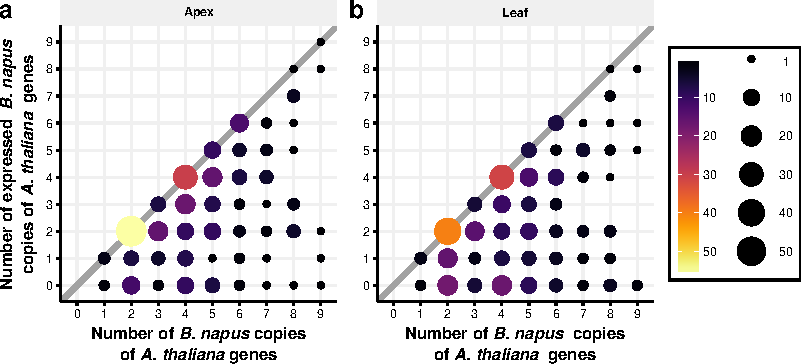
\includegraphics{figuredirectory/14_all_vs_exp_flower_genes.pdf}
\caption{\textbf{Not all copies of flowering time genes are expressed in
\emph{B.~napus}.} As for figure \ref{figure:213:allvsexp}, but only
using \emph{B.~napus} genes that have sequence similarity to annotated
Arabidopsis flowering time genes in the FLOR-ID
database\textsuperscript{288}.}\label{figure:214:allvsexpflower}
\end{figure}

The distributions of \emph{B.~napus} homologue number suggest that genes
involved with the regulation of flowering time have been retained in the
genome. Investigating the regulatory divergence between these homologues
can provide clues as to the evolutionary forces maintaining them in the
genome\textsuperscript{215,223}. In order to assess regulatory
divergence of \emph{B.~napus} genes in a binary manner (expressed versus
not expressed), the number of annotated \emph{B.~napus} homologues of
Arabidopsis genes were compared to the number of those genes that were
expressed during the transcriptomic time series (Figures
\ref{figure:213:allvsexp} and \ref{figure:214:allvsexpflower}). In both
the apex and the leaf, the majority (66~\% in the apex, 70~\% in the
leaf) of Arabidopsis genes have at least one \emph{B.~napus} homologue
that does not exhibit expression during the time series (Figure
\ref{figure:213:allvsexp}). The percentage of Arabidopsis flowering time
genes that have at least one homologue that is not expressed are similar
to the results observed genome-wide (61~\% in the apex, 69~\% in the
leaf) (Figure \ref{figure:214:allvsexpflower}). This indicates
widespread expression divergence among \emph{B.~napus} homologues during
the transcriptomic time series, with the majority of Arabidopsis genes
exhibiting at least one non-expressed homologue in the two tissues
sampled.

\subsection{Expressed copies of flowering time genes exhibit regulatory
divergence during the floral
transition}\label{section:spring:divergence}

\begin{figure}[htbp]
\centering
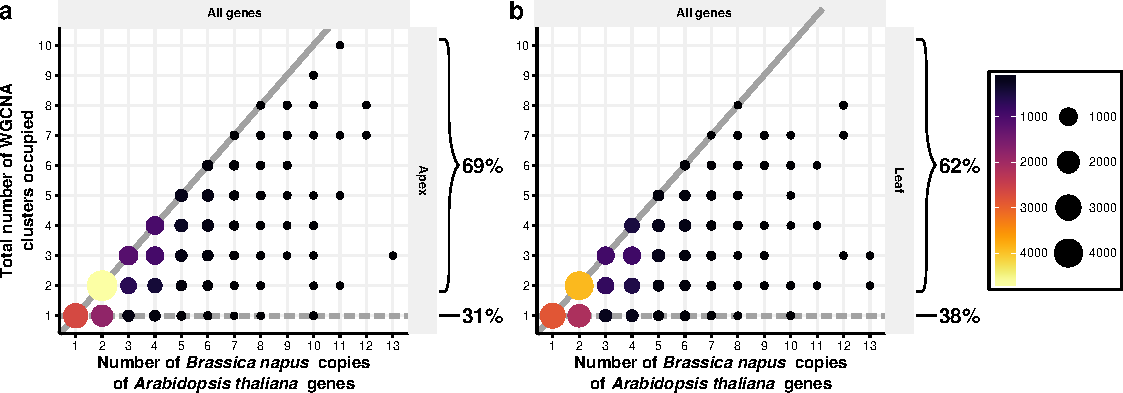
\includegraphics{figuredirectory/15_wgcna_cluster_all_genes.pdf}
\caption{\textbf{The majority of gene homologues in \emph{B.~napus} are
assigned to different regulatory modules.} Regulatory module assignments
for the apex, \textbf{a}, and leaf, \textbf{b}. The size and colour of
the circles indicate the number of data points at that position in the
graph. The thick lines on each graph represent two potential extremes.
The dashed line represents the null hypothesis that all \emph{B.~napus}
copies of an Arabidopsis gene are assigned to the same WGCNA cluster.
The solid line represents the Arabidopsis genes that have
\emph{B.~napus} copies that are each assigned to separate WGCNA
clusters. The percentages indicated on the graph indicate the percentage
of data points that agree, and the percentage that do not agree, with
the null hypothesis. Only \emph{B.~napus} genes with expression above
2.0~FPKM in at least one time point in the transcriptomic time series
and sequence conservation to an annotated Arabidopsis gene were
used.}\label{figure:215:wgcnaall}
\end{figure}

\begin{figure}[htbp]
\centering
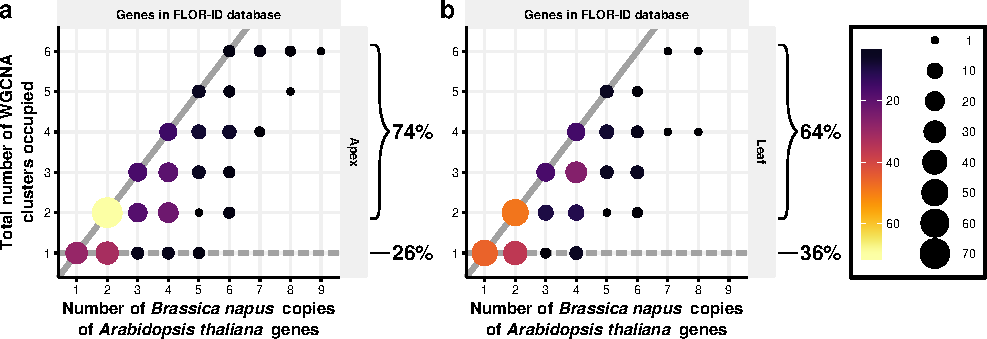
\includegraphics{figuredirectory/16_wgcna_cluster_flower_genes.pdf}
\caption{\textbf{The majority of flowering time gene homologues in
\emph{B.~napus} are assigned to different regulatory modules.} As for
figure \ref{figure:215:wgcnaall}, but only using \emph{B.~napus} genes
that have sequence similarity to annotated Arabidopsis flowering time
genes in the FLOR-ID
database\textsuperscript{288}.}\label{figure:216:wgcnaflower}
\end{figure}

In order to further investigate regulatory divergence between
\emph{B.~napus} homologues of Arabidopsis genes, the behaviour of genes
across the time series was studied. Different hypotheses for the
retention of duplicated genes predict different patterns of
co-regulation between these genes\textsuperscript{209,215,220,223}.
Therefore, by comparing the temporal expression patterns between genes,
the mechanism of retention for the flowering time genes can be
investigated. In order to do this Weighted Gene Co-expression Network
Analysis (WGCNA) was used to identify regulatory
modules\textsuperscript{259}. WGCNA uses normalized expression profiles
across time to cluster genes based on their temporal expression
profiles. Thus, genes that co-regulated will be assigned to the same
cluster, whereas genes genes that have diverged in their temporal
expression will be assigned to different clusters. To assess regulatory
divergence between \emph{B.~napus} homologues, the number of
\emph{B.~napus} homologues of an Arabidopsis gene were compared to the
number of WGCNA clusters those homologues occupy (Figure
\ref{figure:215:wgcnaall}). Assuming that gene dosage leads to
co-regulation of duplicated genes\textsuperscript{223}, the null
hypothesis is that all \emph{B.~napus} homologues of an Arabidopsis gene
would be assigned to the same regulatory module (dashed line in Figure
\ref{figure:215:wgcnaall}). However, if regulatory divergence is
observed with at least one homologue this null hypothesis is inaccurate,
with the extreme situation being that every \emph{B.~napus} homologue
occupies a separate WGCNA cluster (solid diagonal line in Figure
\ref{figure:215:wgcnaall}). Most \emph{B.~napus} homologues exhibit
regulatory divergence (69~\% in the apex, 62~\% in the leaf) which does
not conform to the null hypothesis derived from dosage balance
arguments. This pattern is also observed when just \emph{B. napus}
flowering time genes are considered (Figure
\ref{figure:216:wgcnaflower}). These findings reveal that the majority
of \emph{B. napus} genes have diverged from the expression patterns of
their homologues, calling into question the extent to which gene dosage
effects have maintained these duplicate genes in the genome.

\begin{figure}[htbp]
\centering
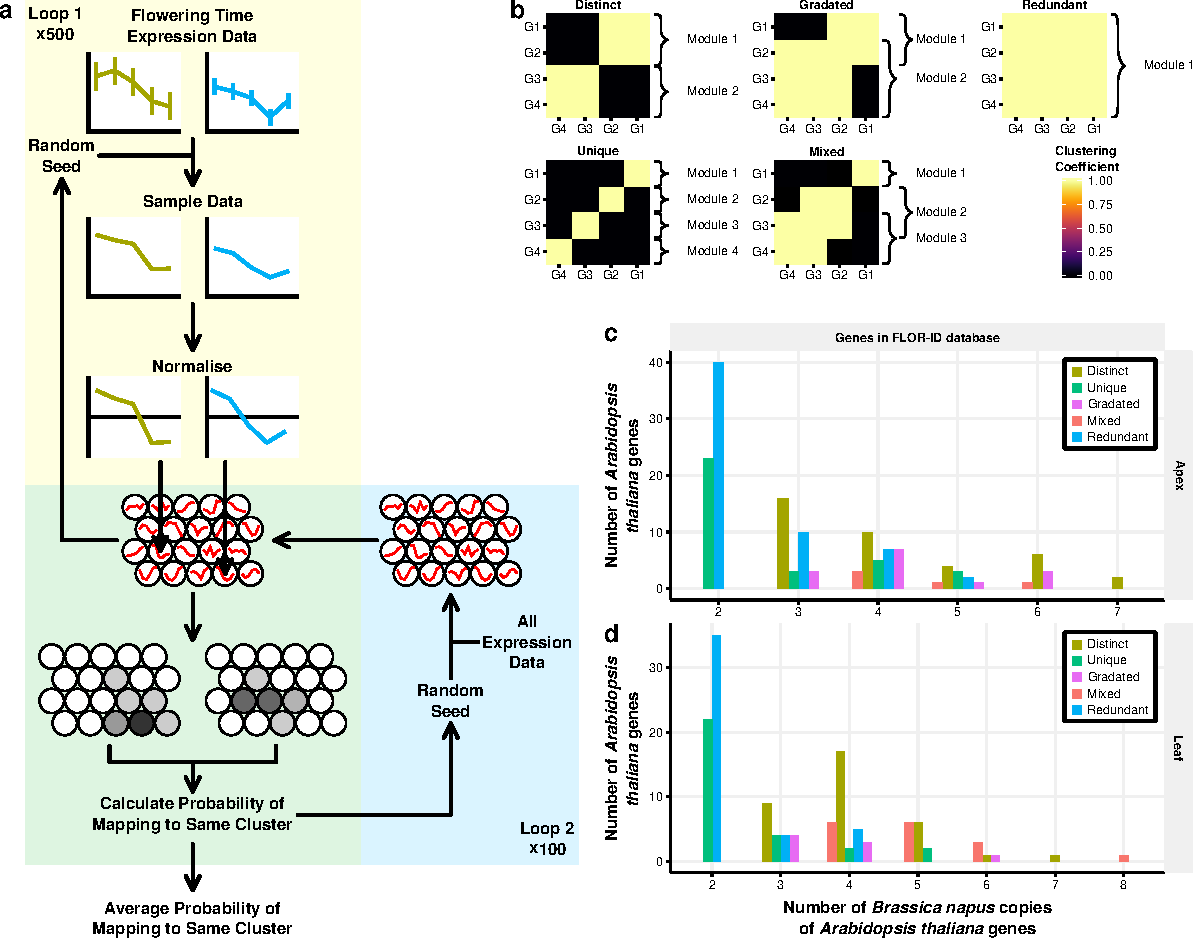
\includegraphics{figuredirectory/18_som_similarity_measure.pdf}
\caption{\textbf{Self-organizing map (SOM) based assessment of
expression trace divergence uncovers widespread regulatory divergence
and subtle patterns of divergence.} \textbf{a} A schematic of the SOM
based clustering approach. The approach consists of two overlapping
sampling loops. In loop 1, expression data from flowering time gene
copies is sampled assuming a Gaussian error model. Sampled expression
traces are zero mean and unit variance normalized and mapped to the SOM.
This procedure is repeated 500 times to give two density plots of where
in the SOM the copies map. These density plots are used to calculate the
probability of the copies mapping to the same SOM cluster. As SOM
clustering has a random component, loop 2 consists of regenerating the
SOM using all expression data and calculating the probability of copies
clustering to the same cluster 100 times. Using this, an average
probability of mapping to the same cluster is calculated.
\emph{Continued on Page
\pageref{figure:218:somsimilaritylegend}}}\label{figure:218:somsimilarity}
\end{figure}

\addtocounter{figure}{-1}

\begin{figure} [t!]
\caption{\emph{Continued from Page \pageref{figure:218:somsimilarity}} \textbf{b} Representations of the five patterns of regulatory module assignment detected by the SOM based method. High clustering coefficients between two different genes indicates that those genes have similar expression traces. Clustering coefficients between a gene and itself represent how robustly a gene maps to the SOM. A \emph{distinct} pattern indicates multiple regulatory modules being identified, with no gene occupying more than one module. A \emph{gradated} pattern represents multiple regulatory modules being detected, but genes occupy multiple modules. \emph{Redundant} patterns occur when only one regulatory module is detected, and all copies of a gene are assigned to that module. \emph{Unique} patterns are a special case of a \emph{distinct} pattern where each copy of a gene is assigned to a different regulatory module. \emph{Mixed} patterns consist of a mixture of \emph{distinct} and \emph{gradated} patterns, where the gene assignment of some modules overlap while others do not show overlap. When assessing the regulatory module assignment, gene copies that do not robustly map to the SOM are removed. \textbf{c and d} The relationships between the number of expressed \emph{B.\ napus} copies of Arabidopsis flowering time genes and the number of different types of regulatory module assignment patterns exhibited by those gene copies. This relationship is calculated using expression data from the apex (\textbf{c}) and the leaf (\textbf{d}).}%missing
\label{figure:218:somsimilaritylegend}
\end{figure}

The regulatory divergence determined using the WGCNA was assessed in a
binary manner; \emph{B. napus} genes are either assigned to the same
cluster or not. However, this approach does not quantify the similarity
between profiles. The consequence of this is genes that exhibit
expression profiles that could be assigned to multiple regulatory
modules will only be assigned to a single module. In addition, the WGCNA
approach does not account for the uncertainty in the RNA-Seq data when
determining module assignment. To overcome these issues, a SOM-based
sampling approach was taken to assess regulatory divergence between
\emph{B. napus} flowering time homologues (Figure
\ref{figure:218:somsimilarity}a). This method accounts for the
uncertainty in the RNA-Seq data by sampling from the data. By counting
the number of sampling iterations in which two genes cluster together,
relative to the total number of sampling iterations, empirical
probabilities of two expression traces mapping to the same SOM cluster
are generated (Figure \ref{figure:218:somsimilarity}a). These
probabilities are normalized to give a clustering coefficient (Methods;
section \ref{section:methods:somclustering}). The higher the
coefficient, the higher the probability of two expression traces mapping
to the same cluster. \emph{B.~napus} copies of Arabidopsis genes are
grouped into regulatory modules based on the clustering coefficients,
with copies that have high clustering coefficients between them being
assigned to the same regulatory module. Unlike some methods of
clustering gene expression profiles, genes have the potential to be
assigned to multiple regulatory modules. This allows more subtle
patterns of divergence to be detected. There are five different possible
patterns of regulatory module assignment using the SOM-based resampling
method (Figure \ref{figure:218:somsimilarity}b). A \emph{distinct}
pattern represents the identification of multiple regulatory modules
whose membership does not overlap. \emph{Gradated} patterns indicate
that multiple regulatory modules were identified, but the membership of
those modules overlap. \emph{Redundant} patterns occur when all
\emph{B.~napus} copies of an Arabidopsis gene are assigned to the same
regulatory module. The \emph{unique} pattern is a special case of the
\emph{distinct} pattern, where only one gene is assigned to each
regulatory module identified. Finally, the \emph{mixed} pattern is
observed when at least three regulatory modules are identified, with
some genes assigned to multiple regulatory modules and others are not.
The benefit of allowing genes to occupy multiple regulatory modules is
that subtle patterns can be detected. For example, copies exhibiting
\emph{gradated} patterns of regulatory module assignment exhibit
intransitivity; although gene A and gene B are in the same regulatory
module, and gene B and gene C are in the same regulatory module, gene A
and gene C are not necessarily mapped to the same module. In this case,
given that gene A and gene C are not in the same module, it is clear
that gene B exhibits a regulatory trace that is intermediate between
gene A and gene C.

To assess the extent of regulatory divergence among \emph{B.~napus}
flowering time gene homologues using the SOM-based method, the
regulatory module assignments were quantified. As with the WGCNA-based
approach, the null hypothesis considered was that of genes exhibiting
co-regulation. In the SOM-based analysis, this hypothesis corresponds to
observing a \emph{redundant} regulatory module assignment. Data from the
developmental time series reveals that as the number of \emph{B.~napus}
copies of an Arabidopsis gene increases, the occurrence of
\emph{redundant} patterns decreases in both the apex and the leaf
(Figures \ref{figure:218:somsimilarity}c and
\ref{figure:218:somsimilarity}d). When three or more copies of a gene
are present, regulatory module patterns over than \emph{redundant} are
observed in the majority of cases in both tissues, with no redundant
patterns seen above 5 copies in the apex or 4 copies in the leaf.
\emph{Unique} patterns were also observed less frequently at higher
numbers of copies, suggesting that as the number of homologues
increases, the more likely it is that those homologues exhibit
regulatory divergence. Therefore, as with the results from the WGCNA
analysis, the null hypothesis ceases to be true for flowering time genes
with five or more copies in the \emph{B. napus} leaf (Figure
\ref{figure:218:somsimilarity}d) or six or more copies in the apex
(Figure \ref{figure:218:somsimilarity}c). An advantage that the
SOM-based analysis has compared to the WGCNA-based analysis is that the
method allows for the detection of \emph{mixed} and \emph{gradated}
patterns. In the apex and leaf, \emph{mixed} and \emph{gradated}
patterns are seen at a lower frequency than \emph{distinct} patterns.
This reveals that genes with intermediary regulatory behaviour are
observed less frequently than genes exhibiting greater divergence in
their expression profiles. Gene copies with intermediate regulatory
behaviour may indicate that particular copies are more susceptible to
regulatory cross-talk than others.

An interesting observation from the SOM-based analysis is the relatively
large number of \emph{distinct} patterns observed at four gene copies
(Figures \ref{figure:218:somsimilarity}c and
\ref{figure:218:somsimilarity}d). To test if this was due to
homoeologous genes displaying similar expression profiles, homoeologue
information was incorporated into the analysis. For the genes for which
homoeologue information was available, the majority (76~\% in apex,
72~\% in leaf) of genes are in the same regulatory module as their
homoeologue. More generally for all expression traces, of 85 pairs of
homoeologues expressed in the apex, 67 (79~\%) are found in the same
regulatory module. In the leaf, 53 of 69 (77~\%) of expressed
homoeologous pairs are found in the same module, with 29 of the
co-regulated pairs being common between the two tissues. The percentage
of Arabidopsis genes with at least two expressed homologues in the apex
(leaf) exhibiting each of the regulatory module assignments are 25~\%
(26~\%) \emph{distinct}, 9~\% (6~\%) \emph{gradated}, 23~\% (23~\%)
\emph{unique}, 39~\% (33~\%) \emph{redundant}, and 3~\% (6~\%)
\emph{mixed}. This reveals that although extensive regulatory divergence
is observed, homoeologous genes still tend to exhibit similar expression
profiles. This suggests that since the formation of \emph{B. napus}
10,000 years ago\textsuperscript{103}, the majority of homoeologous
genes have not diverged in their expression.

\subsection{Conclusions}\label{conclusions-1}

To investigate whether flowering time genes have been retained in the
\emph{B. napus} genome, and the mechanisms by which these gene copies
have been retained, the expression of \emph{B. napus} gene homologues
were compared during the transcriptomic time series. Analysis of the
expression levels of all genes revealed that, on average, the A genome
has a greater proportion of highly expressed genes relative to the C
genome. That this observation becomes less apparent when \emph{B. napus}
genes lacking sequence conservation to an Arabidopsis gene are removed
suggests that the C genome contains a greater number of pseudogenes;
gene models detected by the gene prediction algorithm but that are
transcriptionally silenced. This supports observations that the C genome
contains a higher density of transposons and higher DNA methylation
levels than the A genome\textsuperscript{114}. At the homoeologue level,
biased gene expression was observed towards both genomes, although a
higher number of homoeologue pairs were biased towards the C genome.
This is also consistent with previous observations\textsuperscript{114},
although that biases are observed in both directions proves inconclusive
for determining whether one genome is dominant over the other.

Investigating the expression of flowering time genes in \emph{B. napus}
reveals that these genes exhibit higher retention in the genome relative
to the genome-wide trend (Figure
\ref{figure:212:retentiondistribution}). The majority of Arabidopsis
genes have at least one \emph{B. napus} homologue that lacks expression
during the transcriptomic time series (Figure
\ref{figure:212:retentiondistribution}). This is consistent with the
idea of responsive backup circuits, that posits that duplicate genes can
be retained in the genome, with one copy only expressed when the other
copy becomes non-functional as a result of
mutation\textsuperscript{215,216}. To further investigate this
divergence, WGCNA- and SOM-based clustering approaches were employed to
quantify the extent of divergence between expressed \emph{B.~napus}
homologues. The WGCNA-based analysis revealed extensive regulatory
divergence for all genes, including the subset of flowering time genes.
The SOM-based approach confirmed the observation of flowering time genes
exhibiting regulatory divergence in a manner robust to the calculated
experimental uncertainty. Additionally, the SOM-based analysis reveals
that some copies of flowering time genes exhibit a \emph{gradated}
patterns of regulatory module assignment, representing subtle
differences in regulation. This may be the result of regulatory
cross-talk between the copies, or represents subtle functional
differences that have consequences for the control of flowering time in
\emph{B. napus}. The regulatory divergence observed for the flowering
time genes is counter to the expectations of a gene dosage model for
their retention; namely co-regulation\textsuperscript{220,223}. As the
spatiotemporal expression pattern of a gene plays a crucial role in its
function, this also suggests functional divergence of \emph{B. napus}
flowering time gene homologues. This would therefore suggest that
mechanisms other than gene dosage, such as subfunctionalization,
neofuncionalization, or responsive backup circuits have also contributed
to flowering time gene retention in \emph{B.
napus}\textsuperscript{202,209,215,216,293}.

\section{Regulatory divergence of key floral
integrators}\label{section:spring:floralintegrators}

The main floral pathways that influence flowering are the photoperiod
pathway, the autonomous pathway, the vernalization pathway, the hormone
pathway, and the ageing pathway\textsuperscript{15}. The signals from
these pathways are integrated by a central decision network of floral
integrators (Section \ref{section:intro:floralintegrators}; Figure
\ref{figure:1xx:floralnetwork}). Despite the importance of this network
for determining the timing of the floral transition in
Arabidopsis\textsuperscript{38}, work investigating homologues of these
floral integrators in \emph{Brassica} species is relatively scarce,
especially when compared to the available literature concerning the
vernalization pathway in the crops (section
\ref{section:intro:brassicafloweringgenes}). The work that is available
reveals that the key Arabidopsis floral integrators are present as
multiple copies in the \emph{B. napus} genome, and that sequence
variation exists both between different varieties and between
homologues\textsuperscript{127,148}. For \emph{TFL1}, \emph{FT}, and
\emph{SOC1}, sequence variation between copies has been related to
functional differences between the copies, such as changes in expression
pattern and different effects on plant
phenotype\textsuperscript{149--151,153,154}. However, although these
studies have identified expression pattern differences between \emph{B.
napus} homologues of floral integrators, none have determined which
copies exhibit expression consistent with the regulatory interactions
identified in Arabidopsis. In addition, only in the case of \emph{SOC1}
homologues has the tissue specific expression of the different copies
been assessed\textsuperscript{154}. This is of particular interest given
results from Arabidopsis that suggest that duplicated regulatory
networks will tend to diverge and form parallel regulatory networks that
are distinct in terms of their spatiotemporal
expression\textsuperscript{293}.

To investigate whether \emph{B. napus} homologues of the floral
integrators have diverged in \emph{B. napus}, the expression profiles of
these genes were assessed in the transcriptomic time series for the
spring variety Westar. Every Arabidopsis floral integrator considered
has at least one copy in \emph{B. napus} that exhibits an expression
profile consistent with the expression pattern expected from
observations in Arabidopsis. However, regulatory divergence is also
observed among the integrators, with the degree of divergence varying
based on the gene. Analysing the regulatory patterns exhibited by
\emph{BnSOC1} genes, suggest that some copies respond to the
vernalization treatment, while others do not. This provides evidence
that these genes have subfunctionalized to become responsive to
particular inputs. \emph{BnLFY} genes, however, seem to be acting in a
redundant manner, suggesting that dosage effects may influence the
retention of the additional \emph{BnLFY} genes in the genome. In order
to focus this analysis, only the floral integrator hubs included in the
model of the floral transition by Jaeger et al.
(2013)\textsuperscript{38} will be considered.

\subsection{\texorpdfstring{\emph{FLOWERING LOCUS
T}}{FLOWERING LOCUS T}}\label{section:spring:ft}

\begin{figure}[htbp]
\centering
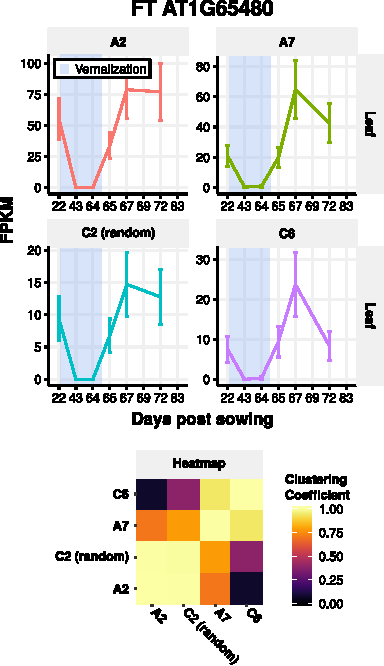
\includegraphics{figuredirectory/23_exp_ft_leaf.pdf}
\caption{\textbf{Expression traces for the \emph{BnFT} genes in the
Westar leaf.} The expression values in FPKM and the 95~\% confidence
intervals of those expression values as computed by Cufflinks are
displayed. A heatmap of the clustering coefficients calculated by the
SOM based method (Section \ref{section:spring:divergence}) is also
displayed. The expression patterns between the four genes are similar,
yet diverge at the final time point, with the A7 and C6 copies
decreasing in expression while the A2 and C2 copies do
not.}\label{figure:223:ftleaf}
\end{figure}

\begin{figure}[htbp]
\centering
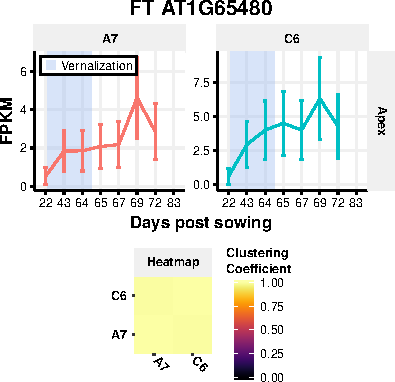
\includegraphics{figuredirectory/25_exp_ft_apex.pdf}
\caption{\textbf{Expression traces for the \emph{BnFT} genes in the
Westar apex.} The expression values in FPKM and the 95~\% confidence
intervals of those expression values as computed by Cufflinks are
displayed. A heatmap of the clustering coefficients calculated by the
SOM based method (Section \ref{section:spring:divergence}) is also
displayed. The A7 and C6 copies exhibit very similar expression traces,
increasing gradually during the time series.}\label{figure:225:ftapex}
\end{figure}

\emph{FT} is a floral activator that is induced in long day conditions
to promote flowering\textsuperscript{20--22}. In Arabidopsis, \emph{FT}
is primarily expressed in the phloem companion cells, with the FT
protein transported in the plant vasculature to the apex to initiate
flowering\textsuperscript{39,41--43}. It is likely that this mechanism
of \emph{FT} action is conserved in
\emph{B.~napus}\textsuperscript{294}. Although the leaf is the primary
expression domain of \emph{FT}, expression of the gene has also been
observed in the shoot apex and the hypocotyl of long day grown
plants\textsuperscript{22,226}, although the biological relevance of
these observations are unknown. In contrast to other studies that found
six copies of \emph{FT} in \emph{B.~napus}\textsuperscript{149,295},
only four copies of \emph{BnFT} were found in the transcriptomic time
series, situated on chromosomes A2, A7, C2, and C6. In previous studies,
two additional copies were found on A7 and C6, with these copies located
in inverted blocks of duplicated sequence\textsuperscript{295}.
Potentially the reason the additional copies of \emph{BnFT} are not
present in the Darmor-\emph{bzh} reference genome is due to a genome
assembly error, caused by the inverted blocks failing to be resolved.

As \emph{FT} is primarily expressed in the leaf in
Arabidopsis\textsuperscript{39,41--43}, the expression of the gene in
this tissue was analysed. The four \emph{BnFT} homologues exhibit a
\emph{gradated} pattern of regulatory module assignment with two
regulatory modules (Figure \ref{figure:223:ftleaf}). All four
\emph{BnFT} genes exhibit moderate expression prior to cold treatment.
During vernalization, \emph{BnFT} gene expression decreases to very low
values, with expression increasing when plants are returned to growth in
warm, long day conditions. Between the penultimate and final time
points, the A7 and C6 copies exhibit a significant decrease in their
expression, while the A2 and C2 copies do not. This decrease in
expression is not as severe for the \emph{BnFT.A7} gene, resulting in
the gene being assigned to both regulatory modules (Figure
\ref{figure:223:ftleaf}). In the leaf, therefore, \emph{BnFT.A2} and
\emph{BnFT.C2} both exhibit a divergent expression trace to
\emph{BnFT.C6}, but \emph{BnFT.A7} shows similarities in its expression
trace with all homologues. This suggests subtle regulatory divergence
between the copies of \emph{BnFT}. Comparing the magnitude of
expression, the A genome copies of \emph{BnFT} are more highly expressed
than the copies on the C genome. \emph{BnFT.A2} is generally 5 fold more
highly expressed across the time series relative to
\emph{BnFT.C2.Random}\footnote{The \emph{B. napus} reference
  genome\textsuperscript{114} constructed sequence scaffolds that were
  joined to generate 19 pseudochromosomes. Scaffolds that mapped to a
  pseudochromosome but could not be oriented were denoted `random'.
  Unmapped scaffolds that could be assigned to the A or C genome were
  denoted `Ann' and `Cnn' respectively. Scaffolds that were not mapped
  during any of these steps were denoted `Unn'.}, while \emph{BnFT.A7}
is 2~-~3 fold more highly expressed than \emph{BnFT.C6}. This genome of
origin bias suggests that the A genome copies potentially influence
flowering to a greater extent than the C genome copies.

To determine whether the \emph{BnFT} genes exhibit tissue specific
expression, the expression of these four genes was analysed in the apex
samples. In the apex, only two of the \emph{BnFT} genes are expressed;
\emph{BnFT.A7} and \emph{BnFT.C6} (Figure \ref{figure:225:ftapex}). As
opposed to the expression pattern observed in the leaf (Figure
\ref{figure:223:ftleaf}), the expression of both copies begins lowly
expressed, gradually increasing during the time series until decreasing
at the final time point. The magnitude of expression of both copies is
similar. These findings suggests that the \emph{BnFT} genes may indeed
have diverged in their spatial expression domains, with \emph{BnFT.A7}
and \emph{BnFT.C6} exhibiting expression in both the leaf and the apex,
whereas \emph{BnFT.A2} and \emph{BnFT.C2.Random} are only expressed in
the leaf. In addition, the expression of the \emph{BnFT} genes in the
apex does not seem to be as responsive to the cold treatment as the
copies in the leaf, suggesting that potentially different pathways are
regulating the expression of \emph{BnFT} genes in the apex relative to
the leaf.

Taking the results from the two tissues together reveals that the A2 and
C2 copies of \emph{BnFT} exhibit similar expression profiles, which are
distinct to those of the A7 and C6 copies. In the leaf, the factor
differentiating these sets of copies is the expression of the genes at
the end of the time series. In Arabidopsis, \emph{FT} will increase in
expression during long days that are inductive to
flowering\textsuperscript{296}. Assuming the same is true in
\emph{B.~napus}, the decrease in expression of \emph{BnFT.A7} and
\emph{BnFT.C6} is unexpected. A potential explanation could be that that
the \emph{BnFT} genes have diverged in their target genes. \emph{FT}
activates the expression of MADS-box containing genes in Arabidopsis to
promote flowering\textsuperscript{45--47}. However, some MADS-box
containing genes have dual roles in floral development, influencing both
the floral transition and floral organ identity\textsuperscript{73,297}
\emph{AGL24}, for example, promotes the formation of the inflorescence
meristem, but is repressed at later points to allow the meristem to
differentiate into floral organs\textsuperscript{297}. It is conceivable
that the A7 and C6 copies of \emph{BnFT} influence the expression of
genes that need to be repressed to allow floral development to occur,
while the A2 and C2 copies do not.

The differences in the magnitude of expression reveal that the A genome
copies are more highly expressed than the C genome copies. Although the
magnitude of expression is not necessarily an indication of the role
that gene plays in the plant, it is interesting to note that variation
in \emph{BnFT.A2}, the most highly expressed copy in the leaf, was found
to be associated with variation in flowering time\textsuperscript{295}.
It is therefore possible that the expression differences observed
between the \emph{BnFT} genes do indeed influence the effect the genes
have on the floral transition.

The decrease in expression of all \emph{BnFT} genes in the leaf during
vernalization is likely a consequence of the change in photoperiod. The
vernalization treatment consisted of short day conditions (8~hours of
light) at 5~°C. When Arabidopsis plants, grown in long day, floral
inductive conditions, are transferred to short day growth conditions,
\emph{FT} expression decreases\textsuperscript{296}. As \emph{B.~napus}
also requires long days for the induction of
flowering\textsuperscript{298}, the expression of \emph{BnFT} during the
vernalization period is consistent with a photoperiod driven repression.
An alternative explanation could be that the \emph{BnFT} genes are
responding to temperature during the vernalization period, given that
both the ambient temperature response\textsuperscript{237} and the
vernalization response\textsuperscript{44} have been implicated in the
control of \emph{FT} in Arabidopsis. However, the ambient temperature
pathway generally responds to less severe changes in
temperature\textsuperscript{299}, and a \emph{BnFLC} gene with an
expression profile consistent with \emph{BnFT} repression during the
cold is not present in Westar (Figure \ref{figure:3xx:flcwesleaf}). This
suggests that all four copies of \emph{BnFT} are influenced by the
photoperiod pathway in the leaf.

Finally, the copies exhibit further regulatory divergence in terms of
tissue specific expression, with A7 and C6 being the only \emph{BnFT}
genes expressed in the apex. A potential explanation for observing these
expression patterns could be from residual leaf and stem tissue
surrounding the apex due to the dissection procedure (section
\ref{section:spring:experimentaldesign}). However, that the expression
profiles are different in the apex relative to the leaf, and that
\emph{BnFT.A2}, the most highly expressed copy in the leaf, is not
observed in the apex implies this is not the case. Although expression
of \emph{FT} has been detected in the apex in
Arabidopsis\textsuperscript{22,226}, it has been shown that \emph{FT}
mRNA is not required in the apex for its role in promoting the floral
transition\textsuperscript{22,42,47}. This suggests that the
\emph{BnFT.A7} and \emph{BnFT.C6} may have a functional role in the apex
that is not related to the floral transition. The lack of a response to
vernalization for the \emph{BnFT} genes in the apex may be due to the
leaf being the primary plant organ that senses photoperiod
signals\textsuperscript{17,18,20--22}. Therefore, potentially the
\emph{Arabidopsis thaliana} \emph{FT} gene has an heretofore unknown
function in the apex that is unrelated to flowering and is conserved in
the A7 and C6 copies of \emph{FT} in \emph{B.~napus}.

\subsection{\texorpdfstring{\emph{APETALA
1}}{APETALA 1}}\label{section:spring:ap1}

\begin{figure}[htbp]
\centering
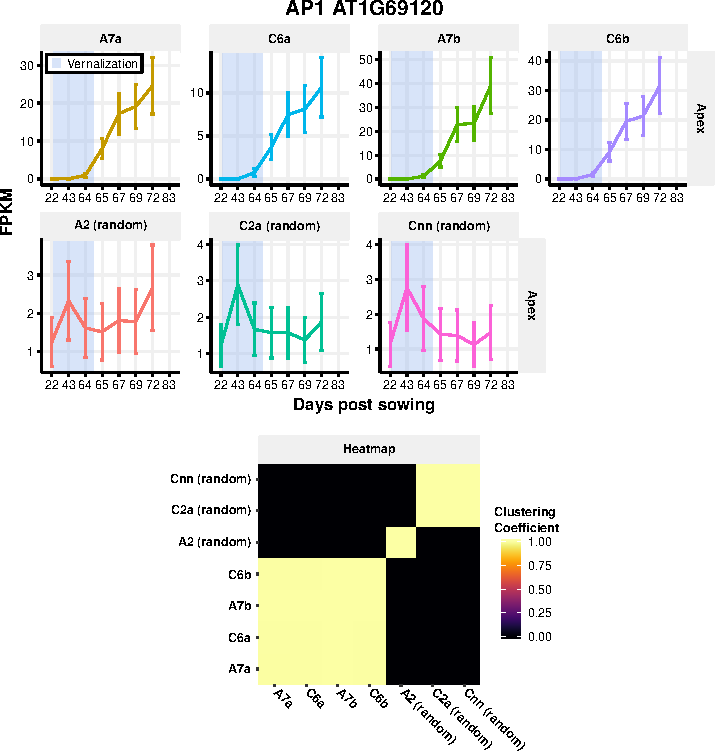
\includegraphics{figuredirectory/26_exp_ap1_apex.pdf}
\caption{\textbf{Expression traces for the \emph{BnAP1} genes in the
Westar apex.} The expression values in FPKM and the 95~\% confidence
intervals of those expression values as computed by Cufflinks are
displayed. A heatmap of the clustering coefficients calculated by the
SOM based method (Section \ref{section:spring:divergence}) is also
displayed. The expression profiles of the four A7 and C6 copies are very
similar to each other. The remaining copies exhibit similar expression
profiles, although \emph{BnAP1.A2.Random} diverges in expression
relative to the C2 and Cnn copies towards the end of the time
series.}\label{figure:226:ap1apex}
\end{figure}

The transcription factor \emph{AP1} controls both meristem identiy and
floral organ specification\textsuperscript{72}. In Arabidopsis,
\emph{AP1} mRNA is uniformly expressed in the floral meristem and later
is localized to the sepals and petals\textsuperscript{72}. No \emph{AP1}
RNA was detected in Arabidopsis roots, stems, leaves, or inflorescence
meristems\textsuperscript{72}, suggesting the shoot apex is the primary
domain of \emph{AP1} expression. Seven copies of \emph{BnAP1} are found
in the transcriptomic time series on chromosomes A2, C2, Cnn, two copies
on A7, and two copies on C6. All copies are only expressed in the apex
tissue, in line with expectations from Arabidopsis\textsuperscript{72}.

The \emph{BnAP1} genes exhibit a \emph{distinct} regulatory module
assignment, with three patterns of regulation (Figure
\ref{figure:226:ap1apex}). The two A7 and two C6 copies display low
expression initially and during the cold, with a steady and gradual
increase until the final time point. The A2, C2a, and Cnn copies show
somewhat similar expression traces, which diverge at the final time
point. All three exhibit an increase in expression at the midpoint of
the vernalization treatment, with a return to pre-treatment expression
levels by the end of cold. The C2a and Cnn copies maintain this
expression level until the end of the time series, while the A2 copy
exhibits a slight increase in expression at the final time point. In
terms of the magnitude of expression, the two pairs of homoeologues on
A7 and C6 have expression levels an order of magnitude higher than the
other copies. Comparing the magnitude of expression between the genes
located on the same chromosome reveals that the copy located further
along the chromosome is more highly expressed on both chromosome A7 and
C6.

The expression of the A7 and C6 copies is most similar to the expression
pattern of \emph{AP1} in Arabidopsis, with expression lacking in
inflorescence meristems and present in floral meristems, increasing as
the meristem increases in size\textsuperscript{72}. This suggests that
these copies are acting redundantly to promote floral meristem identity.
The magnitude differences oberved between copies located on the same
chromosome suggests that the genetic factors controlling this difference
may have been established in an ancestral Brassica before \emph{B.~rapa}
and \emph{B.~oleracea} diverged 0.12~-~3.7~million years
ago\textsuperscript{110,111}. The expression patterns of the A2, C2, and
Cnn copies of \emph{BnAP1} respond to growth in short days and cold
temperatures, which is not typical of \emph{AP1} expression in
Arabidopsis. A potential explanation is provided by the expression
profiles of \emph{BnSVP} genes in \emph{B.~napus} (Figure
\ref{appendixa:svp}; Appendix A). The A4, C4, and Ann copies of
\emph{BnSVP} all exhibit a similar expression response during the
vernalization period as A2, C2, and Cnn. As \emph{AP1} and \emph{SVP}
form dimers\textsuperscript{89} in Arabidopsis, potentially this
response is a consequence of those interactions. It should be noted,
however, that the expression levels of \emph{BnAP1.A2},
\emph{BnAP1.C2a.Random}, and \emph{BnAP1.Cnn.Random} are very low
relative to the A7 and C6 copies, suggesting that they may not play a
strong role in the apex.

\subsection{\texorpdfstring{\emph{SUPPRESSOR OF OVEREXPRESSION OF CO
1}}{SUPPRESSOR OF OVEREXPRESSION OF CO 1}}\label{section:spring:soc1}

\begin{figure}[htbp]
\centering
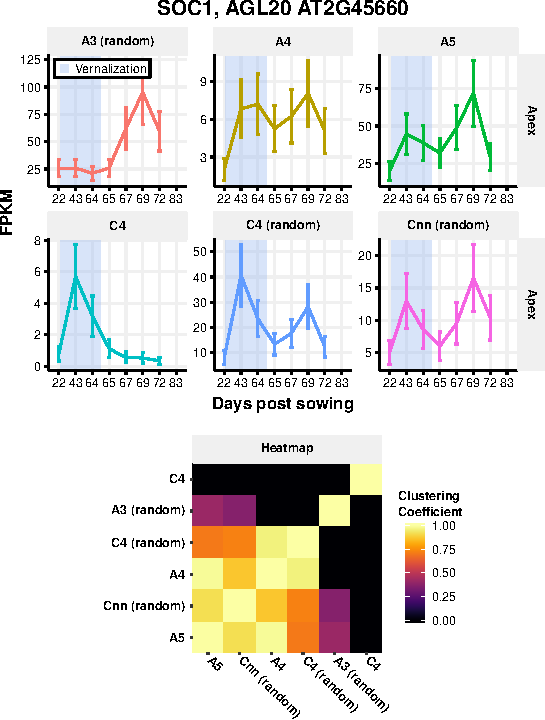
\includegraphics{figuredirectory/27_exp_soc1_apex.pdf}
\caption{\textbf{Expression traces for the \emph{BnSOC1} genes in the
Westar apex.} The expression values in FPKM and the 95~\% confidence
intervals of those expression values as computed by Cufflinks are
displayed. A heatmap of the clustering coefficients calculated by the
SOM based method (Section \ref{section:spring:divergence}) is also
displayed. Expression profiles of \emph{BnSOC1.A4}, \emph{BnSOC1.A5},
\emph{BnSOC1.C4.Random}, and \emph{BnSOC1.Cnn.Random} are similar,
increasing both during vernalization and towards the end of the time
series. The other two copies only exhibit one of these increases, with
\emph{BnSOC1.C4} increasing during vernalization and
\emph{BnSOC1.A3.Random} increasing towards the end of the time
series.}\label{figure:227:soc1apex}
\end{figure}

\emph{SOC1} is a gene in Arabidopsis involved with integrating the
inputs from the photoperiod\textsuperscript{20},
vernalization\textsuperscript{83,84}, hormone\textsuperscript{85} and
age-dependent\textsuperscript{87} floral pathways. Expression of
\emph{SOC1} has been detected in the shoot apical meristem, leaves,
stem, and roots of Arabidopsis plants\textsuperscript{20,83}, but not in
vegetative meristems\textsuperscript{300}. The role of \emph{SOC1} in
flowering is primarily mediated by its expression in the apex, although
expression of the gene in the vasculature has also been found to mediate
an effect on the floral transition\textsuperscript{227}. A number of
regulatory interactions govern the expression of \emph{SOC1} in
Arabidopsis. \emph{SOC1} and \emph{AGL24} regulate each other in a
positive feedback loop\textsuperscript{88}, while \emph{FT}, \emph{CO},
and \emph{FLC} have been implicated in \emph{SOC1} upregulation during a
shift from growth in short day to long day
conditions\textsuperscript{301}. Mutant analysis suggested a hierarchy
of regulation such that \emph{FT} regulates \emph{SOC1}, which in turn
regulates \emph{LFY}\textsuperscript{46}. In \emph{B.~napus} we find six
copies of \emph{BnSOC1} expressed in both the apex and the leaf samples,
located on chromosomes A3, A4, A5, Cnn, and two copies on C4.

As \emph{SOC1} has been found to act in the
apex\textsuperscript{88,227}, the expression of the \emph{BnSOC1} genes
were assessed in this tissue. In the apex, a \emph{distinct} regulatory
module assignment is observed (Figure \ref{figure:227:soc1apex}). The
\emph{BnSOC1.A3.Random} copy and \emph{BnSOC1.A4} copy exhibit different
expression profiles relative to every other \emph{BnSOC1} gene with the
other four gene exhibiting similar expression profiles. There are two
time points in development where the expression of the \emph{BnSOC1}
genes increase. These time points are day 43, during the cold treatment,
and at day 69 post-sowing. However, the increase at these time points
are only observed in some of the copies. The four copies that
demonstrate similar expression profiles (\emph{BnSOC1.A4},
\emph{BnSOC1.A5}, \emph{BnSOC1.Cnn}, and \emph{BnSOC1.C4.Random})
exhibit an increase in expression at both of these time points.
Interestingly, the relative expression between these peaks varies
between the copies. The \emph{BnSOC1.A5} copy is expressed
\textasciitilde{}50~\% higher at the day 69 time point relative to the
time point taken at day 43. Conversely, the same comparison made with
the \emph{BnSOC1.C4.Random} gene reveals that the gene is expressed
\textasciitilde{}25~\% lower at day 69 relative to day 43 of the time
series. The A3 and C4 copies exhibit expression profiles that are
divergent from the other four copies. Expression of the
\emph{BnSOC1.A3.Random} copy is high but stable during the cold
treatment with an increase in expression post-cold peaking at day 69.
This is contrasted by the \emph{BnSOC1.C4} copy that peaks in expression
at the day 43 time point, then returns to very low expression post-cold.
These results suggest that the \emph{BnSOC1} genes respond to the cold
treatment and increase in expression during the floral transition.
However, the different copies exhibit regulatory divergence in terms of
the degree to which they respond to these two signals. When the
magnitude of expression between the copies, \emph{BnSOC1.A3},
\emph{BnSOC1.A5}, and \emph{BnSOC1.C4.Random} exhibit the highest
expression levels. However, even within these genes significant
divergence is observed, with \emph{BnSOC1.A3} and \emph{BnSOC1.A5}
expressed \textasciitilde{}2~fold more highly than
\emph{BnSOC1.C4.Random}. This suggests regulatory divergence in terms of
the magnitude of expression, in addition to expression profile
differences.

\begin{figure}[htbp]
\centering
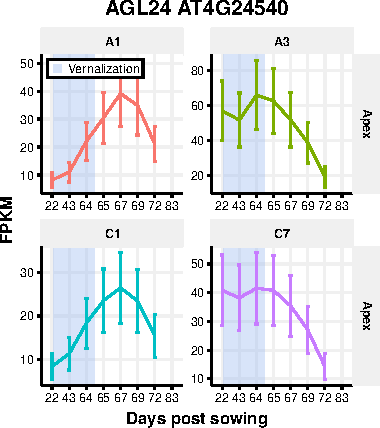
\includegraphics{figuredirectory/29_exp_agl24_apex.pdf}
\caption{\textbf{Expression traces for the \emph{BnAGL24} genes in the
Westar apex.} The expression values in FPKM and the 95~\% confidence
intervals of those expression values as computed by Cufflinks are
displayed. The A3 and C7 copies exhibit a decrease in expression over
the time series while A1 and C1 increase over the time series. Both of
these expression traces are consistent with \emph{BnAGL24} interacting
with \emph{BnSOC1} genes.}\label{figure:229:agl24apex}
\end{figure}

The expression of \emph{SOC1} in the Arabidopsis apex is proposed to
occur in a positive feedback loop with the gene
\emph{AGL24}\textsuperscript{88}. To test if this interaction is also
observed in \emph{B. napus}, the expression profiles of \emph{BnAGL24}
were compared to those of \emph{BnSOC1}. Four copies of \emph{BnAGL24}
are expressed in the apex, situated on chromosomes A1, C1, A3, and C7
(Figure \ref{figure:229:agl24apex}). The expression of the A1 and C1
genes increases gradually during the time series, decreasing at the
final time points. The A3 and C7 copies, however, show an almost inverse
expression profile; highly expressed initially with a gradual decrease
during the time series. Comparing these expression profiles with those
of \emph{BnSOC1} reveals that the expression of the \emph{BnAGL24.A1}
and \emph{BnAGL24.C1} genes is consistent with with regulatory feedback
with all \emph{BnSOC1} genes except the C4 copy. Likewise,
\emph{BnAGL24.A3} and \emph{BnAGL24.C7} potentially regulate all
\emph{BnSOC1} genes except \emph{BnSOC1.A3.Random}. The expression
profiles of \emph{BnAGL24} suggest, therefore, that the positive
feedback loop may exist between these genes in \emph{B. napus}, but copy
specificity is observed.

\begin{figure}[htbp]
\centering
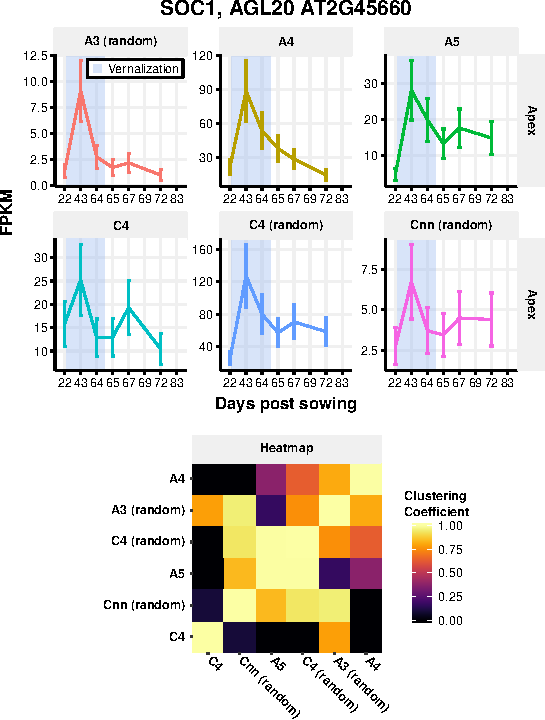
\includegraphics{figuredirectory/28_exp_soc1_leaf.pdf}
\caption{\textbf{Expression traces for the \emph{BnSOC1} genes in the
Westar leaf.} The expression values in FPKM and the 95~\% confidence
intervals of those expression values as computed by Cufflinks are
displayed. A heatmap of the clustering coefficients calculated by the
SOM based method (Section \ref{section:spring:divergence}) is also
displayed. The expression profiles of all \emph{BnSOC1} genes increases
during vernalization. The expression profiles exhibit a complex
\emph{gradated} pattern of regulatory module assignment, with the
difference between pre- and post-cold expression levels being the main
differentiator.}\label{figure:228:soc1leaf}
\end{figure}

To determine if the \emph{BnSOC1} genes exhibit tissue specific
regulatory divergence, the expression of the genes was assessed in the
leaf. The same six copies of \emph{BnSOC1} are expressed in the leaf as
in the apex. The \emph{BnSOC1} copies in the leaf exhibit a
\emph{gradated} regulatory module assignment, suggesting subtle
differences between the expression profiles of the \emph{BnSOC1} genes
(Figure \ref{figure:228:soc1leaf}). A commonality between the expression
patterns is the response to the cold treatment, with all six of the
copies peaking in expression at day 43 of the time series, halfway
through vernalization. The differentiating factor between the expression
profiles of \emph{BnSOC1} genes in the leaf is the difference between
the pre- and post-cold expression levels. At one extreme, the
\emph{BnSOC1.A5} and \emph{BnSOC1.C4} genes are expressed
\textasciitilde{}2~fold higher post-cold relative to before the
treatment. This is in contrast to the \emph{BnSOC1.A3} and
\emph{BnSOC1.A4} genes, that are expressed at similar levels before and
after the treatment. This findings suggests that all copies of
\emph{BnSOC1} respond to the cold treatment when it is occurring, but
only some copies continue to respond to the treatment when it ends. As
observed in the apex, expression magnitude differences are also observed
between the copies in the leaf. \emph{BnSOC1.A4} and
\emph{BnSOC1.C4.Random} exhibit the highest expression levels, with the
next most highly expressed copy, \emph{BnSOC1.A5}, expressed 3~-~4 fold
lower.

These results from both the apex and leaf suggest regulatory divergence
of the \emph{BnSOC1} genes, both in terms of expression profile and
tissue specific expression. From Arabidopsis it has been shown that
\emph{SOC1} is activated in the apex by the photoperiod pathway
downstream of \emph{FT} and \emph{CO}\textsuperscript{20,46,82,301,302}.
Based on the expression of \emph{BnFT} (Figure \ref{figure:223:ftleaf}),
\emph{BnSOC1.A3.Random} is the only \emph{BnSOC1} gene with an
expression pattern consistent with this regulation (Figure
\ref{figure:227:soc1apex}). This is also supported by the
\emph{BnSOC1.A3.Random} copy exhibiting the highest expression of all
the copies in the apex. Therefore, \emph{BnSOC1.A3.Random} is a good
candidate for carrying out the role of \emph{SOC1} in \emph{B.~napus}.

All other \emph{BnSOC1} genes in the apex, and all \emph{BnSOC1} genes,
including the A3 copy in the leaf, exhibit an increase in expression
during the cold treatment. This is interesting given that in
Arabidopsis, \emph{SOC1} expression is activated during vernalization by
both \emph{FLC} dependent\textsuperscript{44,84} and
independent\textsuperscript{85} pathways. Although Westar is a spring
variety, it still exhibits a weak vernalization
response\textsuperscript{234}, and a number of \emph{BnFLC} genes
exhibit expression consistent with \emph{BnSOC1} activation in the leaf
and apex (Figures \ref{figure:3xx:flcwesleaf} and
\ref{figure:3xx:flcwesapex}). Therefore, potentially the vernalization
response is mediating the cold-induced increase in \emph{BnSOC1}
expression. This hypothesis is strengthened by the observation that some
\emph{BnSOC1} genes in the leaf do not return to pre-cold levels after
the cold, a response that would be expected from vernalization sensitive
genes.

Taken together, the transcriptomic time series reveals regulatory
divergence between \emph{SOC1} homologues in \emph{B.~napus}, which
seems to be tissue specific. In the apex, different expression profiles
suggest that different copies of \emph{BnSOC1} are sensitive to
different environmental inputs. The relative magnitudes of expression
between \emph{BnSOC1} genes differ depending on the tissue, with
\emph{BnSOC1.A3.Random} and \emph{BnSOC1.A5} copies being most highly
expressed in the apex and \emph{BnSOC1.C4.Random} and \emph{BnSOC1.A4}
in the leaf. Both of these examples of regulatory divergence suggest
that the \emph{BnSOC1} genes have subfunctionalized, both in terms of
the inputs they respond to and the tissues in which they are expressed.

\subsection{\texorpdfstring{\emph{FD}}{FD}}\label{section:spring:fd}

\begin{figure}[htbp]
\centering
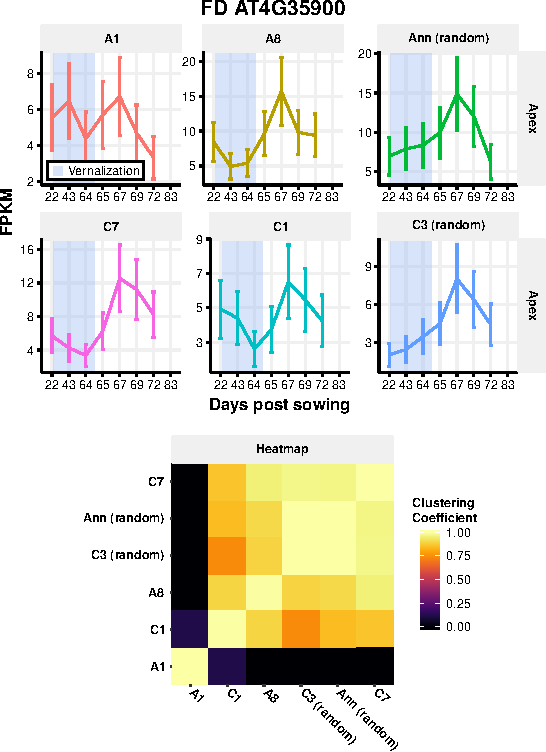
\includegraphics{figuredirectory/30_exp_fd_apex.pdf}
\caption{\textbf{Expression traces for the \emph{BnFD} genes in the
Westar apex.} The expression values in FPKM and the 95~\% confidence
intervals of those expression values as computed by Cufflinks are
displayed. A heatmap of the clustering coefficients calculated by the
SOM based method (Section \ref{section:spring:divergence}) is also
displayed. Expression of five \emph{BnFD} genes exhibit similar
expression profiles, increasing in expression during the time series
until day 67, and then decreasing. \emph{BnFD.A1} exhibits a different
response, staying approximately constant in expression throughout the
time series.}\label{figure:230:fdapex}
\end{figure}

The FD protein is a bZIP transcription factor that interacts with FT and
TFL1 proteins\textsuperscript{38,45,47} to mediate their effect on the
floral transition. \emph{FD} expression in Arabidopsis is highly
expressed at the shoot apex, does not exhibit circadian oscillations or
photoperiod dependent expression, with \emph{FD} expression decreasing
soon after \emph{AP1} expression begins to
increase\textsuperscript{45,47}. The upregulation of \emph{FD} was found
to be mediated by LFY, with two LEAFY binding sites being found in the
\emph{FD} promoter\textsuperscript{38}. In the transcriptomic time
series there are six copies of \emph{BnaFD} expressed in the apex,
situated on chromosomes A1, A8, Ann, C1, C3, and C7.

The expression of \emph{FD} in Arabidopsis is primarily in the
apex\textsuperscript{45,47}. Investigating the expression of \emph{BnFD}
genes in the apex reveals a \emph{distinct} regulatory module assignment
(Figure \ref{figure:230:fdapex}). Five of the six copies have similar
expression profiles to each other These copies, consisting of the A8,
Ann, C7, C1, and C3 copies, are relatively lowly expressed before and
during cold and increase in expression after vernalization. After
peaking in expression at day 67 of the time series, these genes decrease
in expression. Some slight variation in the expression profiles of these
copies is observed at the initial time points, with \emph{BnFD.C1}
exhibiting a decrease during the cold. This is reflected in the slightly
lower clustering coefficients between \emph{BnFD.C1} and the other
copies assigned to the same regulatory module (Figure
\ref{figure:230:fdapex}). Whether this difference is biologically
relevant, however, would need further validation. Comparing the
magnitude of expression between these five copies reveals that the
\emph{BnFD.C1} and \emph{BnFD.C3.Random} are more lowly expressed than
the other copies. The final copy, \emph{BnFD.A1} exhibits a relatively
noisy expression trace throughout the entire time series. This data
suggests that, aside from the \emph{BnFD.A1} copy, the \emph{BnFD} genes
have not diverged significantly from one another.

The expression of the \emph{BnFD} genes exhibits very similar expression
patterns as the \emph{FD} gene in Arabidopsis; apex specific growth with
an increase in expression during the floral
transition\textsuperscript{45,47}. The timing of the decrease in
\emph{FD} expression after the day 67 post sowing time point corresponds
with the increase in four \emph{AP1} copies (Figure
\ref{figure:226:ap1apex}), as observed in
Arabidopsis\textsuperscript{45}, and also with the increase in
\emph{BnLFY} gene expression (Figure \ref{figure:231:lfyapex}), which is
also consistent with the direct repression of \emph{FD} by
\emph{LFY}\textsuperscript{38}. Therefore, five of the six \emph{BnaFD}
copies seem to be regulated in a similar manner to \emph{FD} in
Arabidopsis. The expression levels of all six of the copies of
\emph{BnaFD} are relatively similar in the plant. Both the similar
expression patterns and the similar expression magnitudes suggest that
the \emph{BnFD} genes may have been maintained in the \emph{B. napus}
genome due to gene dosage effects.

\subsection{\texorpdfstring{\emph{LEAFY}}{LEAFY}}\label{section:spring:lfy}

\begin{figure}[htbp]
\centering
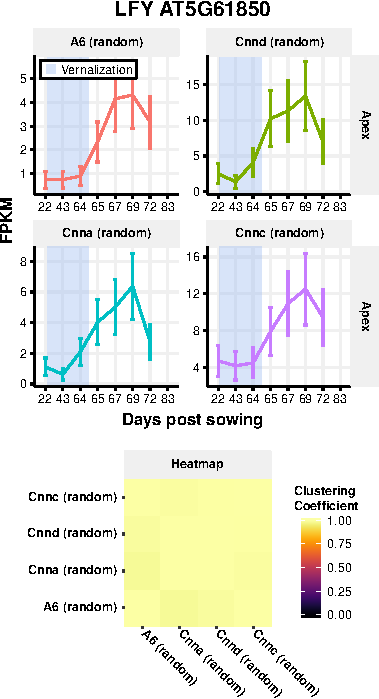
\includegraphics{figuredirectory/31_exp_lfy_apex.pdf}
\caption{\textbf{Expression traces for the \emph{BnLFY} genes in the
Westar apex.} The expression values in FPKM and the 95~\% confidence
intervals of those expression values as computed by Cufflinks are
displayed. A heatmap of the clustering coefficients calculated by the
SOM based method (Section \ref{section:spring:divergence}) is also
displayed. All copies of \emph{BnaLFY} exhibit a similar expression
profile, with low initial expression and an increase in expression after
vernalization.}\label{figure:231:lfyapex}
\end{figure}

\emph{LFY} is a transcription factor that acts synergistically with
\emph{AP1}\textsuperscript{78} to promote the floral transition and
specifiy the determinacy of the floral meristem\textsuperscript{59}. The
gene is expressed in the floral primordia in Arabidopsis and increases
during flower development\textsuperscript{78}, promoting the expression
of other floral integrators such as \emph{AP1}\textsuperscript{61--63}
and \emph{TFL1}\textsuperscript{64}. In the \emph{B.~napus} genome, four
copies of the gene are found, one on chromosome A6, and three assigned
to the C genome but not to a particular chromosome in the
Darmor-\emph{bzh} reference genome.

The four copies of \emph{BnLFY} are only expressed in the Westar apex.
The four copies of \emph{BnLFY} exhibit a \emph{redundant} regulatory
module assignment, with all copies exhibiting low expression initially
and increasing in expression after vernalization (Figure
\ref{figure:231:lfyapex}). At the final time point, a decrease in
expression is observed. This expression profile, increasing during the
floral transition, is consistent with the expression of \emph{LFY} in
Arabidopsis\textsuperscript{69}. Both the expression traces and the
apex-specific expression is consistent with the expression of \emph{LFY}
in Arabidopsis, with a gradual increase during development until
flowering\textsuperscript{69,78}.

The expression traces of the \emph{BnLFY} genes are consistent with the
regulatory interactions observed for \emph{LFY} in Arabidopsis. Five of
the six \emph{BnaSOC1} genes expressed in the apex exhibit a peak in
expression at day 69 (Figure \ref{figure:227:soc1apex}), in agreement
with \emph{LFY} being regulated by \emph{SOC1}\textsuperscript{46,67}.
The expression of certain \emph{BnaAP1} and \emph{BnTFL1} genes is also
consistent with \emph{BnaLFY} mediated regulation (Figures
\ref{figure:226:ap1apex}, \ref{figure:232:tfl1apex}), as has been
observed in Arabidopsis\textsuperscript{61--64}. This evidence suggests
that the \emph{BnaLFY} genes are similarly regulated to their homologue
in Arabidopsis, and that the regulatory roles elucidated for \emph{LFY}
in Arabidopsis seem to be conserved in \emph{B.~napus}.

The co-regulation of the \emph{BnaLFY} genes is consistent with the gene
balance hypothesis\textsuperscript{220,223}. Dosage balance is also
consistent with observations in Arabidopsis. The \emph{LFY} null
mutation was found to be haploinsufficient under short day
conditions\textsuperscript{70}, while insertion of additional copies of
\emph{LFY} into the Arabidopsis genome altered the flowering time of the
transformed plants, with an additional shortening of the flowering time
observed with each additional copy of \emph{LFY}\textsuperscript{69}.
These findings suggest that potentially the copies of \emph{BnaLFY} have
been maintained in the \emph{B.~napus} genome as their loss, or an
alteration of their expression, results in a change in flowering time. A
prediction that arises from this is that a \emph{B.~napus} plant lacking
a copy of \emph{BnaLFY} would have later flowering. \emph{LFY} has a
dual role in both determining the timing of the floral transition and
mediating correct floral patterning\textsuperscript{59}. Assuming that
the copies of \emph{BnaLFY} are redundant, a single inactive copy could
potentially alter flowering time without altering floral patterning, due
to the other copies being able to complement the inactive copy. These
findings could therefore provide a potential avenue for altering
flowering time in \emph{B.~napus}.

\subsection{\texorpdfstring{\emph{TERMINAL FLOWER
1}}{TERMINAL FLOWER 1}}\label{section:spring:tfl1}

\begin{figure}[htbp]
\centering
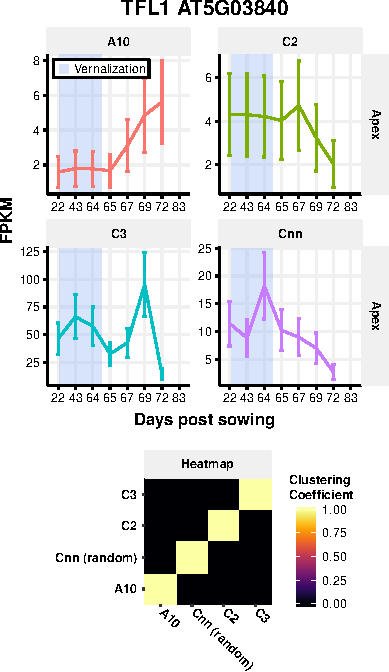
\includegraphics{figuredirectory/32_exp_tfl1_apex.pdf}
\caption{\textbf{Expression traces for the \emph{BnTFL1} genes in the
Westar apex.} The expression values in FPKM and the 95~\% confidence
intervals of those expression values as computed by Cufflinks are
displayed. A heatmap of the clustering coefficients calculated by the
SOM based method (Section \ref{section:spring:divergence}) is also
displayed. The \emph{BnTFL1} genes exhibit total divergence in their
expression profiles, with the C genome copies of the gene being more
highly expressed than the A genome copies.}\label{figure:232:tfl1apex}
\end{figure}

\emph{TFL1} acts in an antagonistic manner to \emph{FT} in
Arabidopsis\textsuperscript{48}, with the gene maintaining inflorescence
meristem identity by limiting the expression of \emph{AP1} and
\emph{LFY}\textsuperscript{51--53}. The expression domain is just below
the growing meristem at the apex, and also in the axillary
meristems\textsuperscript{53,228}. The expression is initially low, with
an increase when the floral transition
occurs\textsuperscript{50,53,54,228}. In agreement with previous
studies\textsuperscript{148,149}, four \emph{BnTFL1} genes were
identified in the transcriptomic time series on chromosomes A10, C2, C3,
and Cnn.

The four \emph{BnTFL1} genes exhibit a \emph{unique} pattern of
regulatory module assignment (Figure \ref{figure:232:tfl1apex}), with
each gene assigned to a separate module. The \emph{BnTFL1.A10} copy is
very lowly expressed initially and remains at that level until after the
cold treatment. From the day 67 time point onwards, the expression of
this copy increases until the final time point. Conversely, the
\emph{BnTFL1.C2} copy effectively exhibits the inverse response, with
expression before, during and after the cold treatment being
comparatively high before decreasing after the day 67 time point.
\emph{BnTFL1.C3} is the most highly expressed copy of \emph{BnTFL1},
with expression levels an order of magnitude higher than the A10 and C2
copies. The expression of the C3 copy increases during vernalization
with a return to pre-cold levels when plants are transferred back to
warm, long day growth conditions. The copy increases in expression to a
peak at day 69 of the time series, before decreasing in expression at
the final time point. Finally, the \emph{BnTFL1.Cnn.Random} copy shows a
transient peak of expression towards the end of vernalization, with a
continued decrease in expression until the final time point after.

The expression profiles of \emph{BnTFL1.A10} and \emph{BnTFL1.C3} are
most consistent with the expression of \emph{TFL1} in Arabidopsis, as
both show increasing expression during the floral
transition\textsuperscript{50,53,54,228}. These copies differ in their
behaviour during the cold treatment and at the final time point. In
Arabidopsis, the floral structure is indeterminate and this requires
continued expression of \emph{TFL1} at the apex\textsuperscript{50}.
This pattern of expression is exhibited most clearly by
\emph{BnTFL1.A10}, as \emph{BnTFL1.C3} decreases in expression at the
final time point. An explanation for this decrease may be due to
\emph{BnTFL1.C3} only maintaining the inflorescence meristem identity
early in development, with this role performed by another gene later in
development.

Comparing the expression of \emph{BnTFL1.C3} and \emph{BnTFL1.A10} to
\emph{BnAP1} and \emph{BnLFY}, the mutual antagonism observed between
these genes in Arabidopsis\textsuperscript{51--53,64} is not seen
between the \emph{B.~napus} homologues of these genes. This is
potentially due to the apex sampling procedure (section
\ref{section:spring:experimentaldesign}) not separating the expression
domains of these genes\textsuperscript{50}. However, it is interesting
that both \emph{BnTFL1.C3} and the \emph{BnaLFY} genes (Figure
\ref{figure:231:lfyapex}) exhibit a decrease in expression at the final
time point, given the mutual antagonism of the genes in Arabidopsis. The
reduction in \emph{BnLFY} activity potentially results in less
\emph{BnTFL1.C3} being required to maintain the inflorescence meristem
state, or vice versa. The regulatory antagonism between \emph{BnTFL1},
\emph{BnAP1} and \emph{BnLFY} might be manifested in the repression of
\emph{BnTFL1.Cnn.Random} and \emph{BnTFL1.C2} towards the end of the
time series. The expression profiles of the four \emph{BnTFL1} copies
reveals that genes have diverged from each other in terms of regulation,
and suggests that dosage effects have not influenced the retention of
\emph{BnTFL1} genes in the \emph{B.~napus} genome.

\subsection{Conclusions}\label{conclusions-2}

The floral integrators in Arabidopsis are integral to the interpretation
of environmental signals to accurately coordinate the floral
transition\textsuperscript{38}. Whether the homologues of these
Arabidopsis floral integrators have retained the same function in
\emph{B.~napus} was previously only understood for relatively few
examples\textsuperscript{127,148--151,153,154}. This work has been
complicated by Arabidopsis floral integrators often having multiple
homologous genes in the \emph{B.~napus} genome\textsuperscript{127}. To
investigate whether the homologues of Arabidopsis floral integrators
have expression profiles consistent with their function in the model
species, the expression of \emph{B.~napus} floral genes was assessed in
the transcriptomic time series. For all six of the floral integrators
examined, at least one \emph{B.~napus} homologue exhibited an expression
profile consistent with retaining a function similar to its Arabidopsis
homologue. This suggests a general conservation of the gene regulatory
network in \emph{B.~napus} relative to Arabidopsis. Testing these
candidates could be achieved by expressing the gene in Arabidopsis
mutants for the gene, as has been done to investigate the efficacy of
homologous \emph{B. napus} flowering time genes
previously\textsuperscript{141}

An advantage of assessing gene expression for all genes simultaneously
is that regulatory interactions known to exist between the floral
integrators in Arabidopsis can be investigated in \emph{B.~napus}. For
example, \emph{SOC1} is upregulated by \emph{FT} in
Arabidopsis\textsuperscript{20,46,82,301,302}. That five of the six
\emph{BnSOC1} genes are upregulated during vernalization (Figure
\ref{figure:227:soc1apex}), when all four \emph{BnFT} genes exhibit very
low expression (Figure \ref{figure:223:ftleaf}), indicates that these
\emph{BnSOC1} genes are not upregulated as a result of \emph{FT}
expression. This in turn makes the one \emph{BnSOC1} gene that does not
increase during the cold, \emph{BnSOC1.A3.Random}, the best candidate
for exhibiting the role of \emph{SOC1} in \emph{B.~napus}.

Finally, different patterns of divergence suggest different selective
pressures may be acting on the \emph{B.~napus} floral integrator genes,
despite the genes being involved with the same regulatory pathway in
Arabidopsis. Co-regulation of floral integrators suggest that gene
dosage effects may be playing a role\textsuperscript{223}. This is
particularly true for \emph{BnLFY}, where dosage effects have also been
demonstrated in Arabidopsis\textsuperscript{69,70}. However, from the
observed divergence it is also clear that subfunctionalization,
neofuncionalization, or the evolution of responsive backup circuits have
also influenced gene retention\textsuperscript{202,209,215,216,293}.
These different scenarios could be tested, for example, by identifying
lines that have non-functional versions of particular floral integrator
genes and investigating how the expression profiles of the remaining
floral integrators are different in those lines.

\section{Sequence divergence between copies of two floral
integrators}\label{section:spring:sequence}

Comparative analysis of the gene DNA sequence of homologous genes in
\emph{Brassica} crops has been used to reveal divergence between the
copies. A analysis of \emph{Brassica} homologues of \emph{FLC} found
variation in the promoter of the gene, including some copies lacking a
region of the promoter important for the expression of the gene in
Arabidopsis\textsuperscript{137}. For \emph{FT} homologues in
\emph{B.~napus} and \emph{B.~oleracea}, a transposable element and a
retro-element in the upstream promoter of the gene on chromosome C2 was
correlated with a lack of expression relative to the other copies of the
gene\textsuperscript{150}. Among \emph{BnTFL1} genes, sequence variation
was identified within the first intron of the gene and in the 3'
regulatory regions\textsuperscript{148}. Other studies investigating
sequence changes have instead focussed on polymorphisms between
varieties, identifying regions of sequence important for gene
function\textsuperscript{127,136,151,153,154}. A common theme between
these analyses is that the amino acid sequences of the analysed
homologues are often very similar\textsuperscript{137,148,154}. In the
case of \emph{BnTFL1} genes, for example, a maximum of 5 amino acid
differences between the homologues was identified\textsuperscript{148}.
However, it has been shown that in Arabidopsis that it only takes a
single amino acid substitution to confer FT-like function onto TFL1
proteins, and vice versa\textsuperscript{57}. Therefore, although the
observed differences between \emph{B.~napus} genes may be minor, they
have the potential to severely impact the function of the gene.

The transcriptomic time series allows sequence differences between
\emph{B.~napus} floral integrators to be viewed in the context of gene
expression during the floral transition. To illustrate how the
transcriptomic time series can be used to facilitate insights on
sequence divergence, two case studies will be considered. For
\emph{BnTFL1} genes, sequence divergence downstream of the gene, in
regions identified as cis-regulatory elements, correlates with the
expression divergence observed between the genes during the time series.
In the case of \emph{BnFD}, sequence polymorphisms within the bZIP
domain are predicted to alter the dimerization affinity of the genes.
The observed sequence differences in bZIP proteins are also identified
in other species, suggesting that this form of divergence is common
among duplicated bZIP proteins. Given that the \emph{BnFD} genes are
co-regulated during the time series, modelling studies reveal that the
observed sequence divergence may impact the expression of genes
regulated by FD.

\subsection{\texorpdfstring{\emph{BnTFL1} cis-regulatory
elements}{BnTFL1 cis-regulatory elements}}\label{section:spring:tfl1regulation}

Cis-regulatory elements downstream of the \emph{TFL1} gene in
Arabidopsis have been found to direct different aspects of gene
regulation\textsuperscript{303}. In the study by Serrano-Mislata et al.
(2016), regions of sequence conservation between the Arabidopsis
\emph{TFL1} and homologues in \emph{Arabidopsis lyrata}, \emph{Capsella
bursa-pastoris}, \emph{B. rapa}, and \emph{Leavenworthia crassa} were
identified up- and downstream of the gene. Further analysis of these
regions determined that these areas of sequence conservation
corresponded to cis-regulatory elements. Interestingly, different
regions were found to influence \emph{TFL1} expression in different
ways. For example, one region identified 1.0~-~1.3 kilobases (kb)
downstream of the gene was required for \emph{TFL1} expression in the
vegetative meristem, while another region situated 1.6~-~2.2 kb
downstream of the gene was required for gene expression in lateral
meristems\textsuperscript{303}. These results are particularly
interesting given the conservation of these cis-regulatory elements
between Arabidopsis and \emph{B.~rapa}\textsuperscript{303}, and
previous identification of between homologue variation in the 3'
regulatory regions of \emph{BnTFL1} genes\textsuperscript{148}.

\subsubsection{\texorpdfstring{Cis-regulatory element variation
downstream of \emph{BnTFL1} genes potentially explain observed
regulatory
divergence}{Cis-regulatory element variation downstream of BnTFL1 genes potentially explain observed regulatory divergence}}\label{section:spring:tfl1conservation}

\begin{figure}[htbp]
\centering
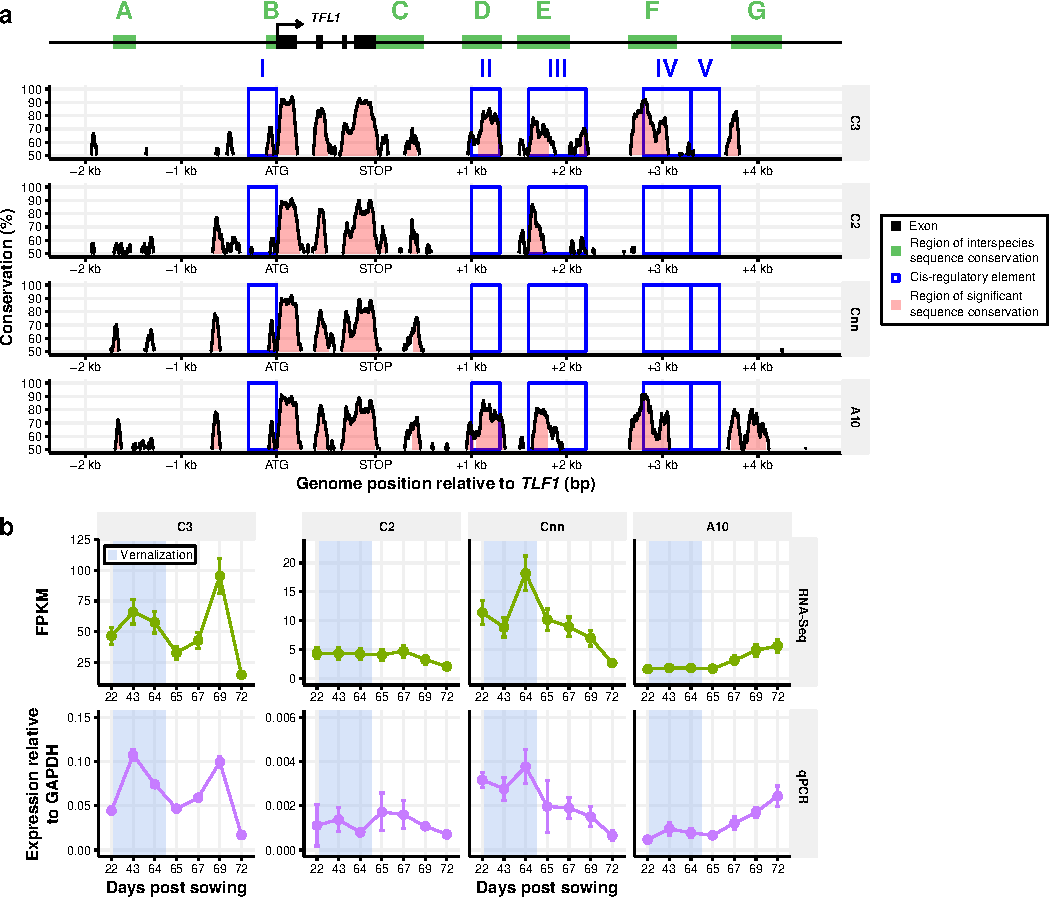
\includegraphics{figuredirectory/33_sequence_conservation_qpcr.pdf}
\caption{\textbf{Sequence analysis reveals that cis-regulatory modules
identified in Arabidopsis are not present downstream of some
\emph{BnTFL1} genes.} \textbf{a} The degree of sequence conservation
between the \emph{BnTFL1} genes and \emph{TFL1}. Sequence alignment and
conservation calculations were performed using the mVISTA
server\textsuperscript{304,305} with a sliding window size of 100~bp.
The seven regions of high interspecies sequence conservation (green
bars) and the five cis-regulatory regions (blue boxes) identified by
Serrano-Mislata et al. (2016) are shown relative to the \emph{TFL1} gene
model\textsuperscript{303} (black bars). The labelling of these regions
follows the same conventions as the previous study. The pink shaded
areas under the sequence conservation curves are regions above 70~\%
sequence conservation. Genomic position upstream and downstream of the
\emph{AtTFL1} gene copies are given relative to the ATG and STOP codon
sites respectively. \emph{Continued on Page
\pageref{figure:233:tfl1conservationlegend}}}\label{figure:233:tfl1conservation}
\end{figure}

\addtocounter{figure}{-1}

\begin{figure} [t!]
\caption{\emph{Continued from Page \pageref{figure:233:tfl1conservation}} \textbf{b} The unnormalized expression profiles for the *BnTFL1* genes determined through RNA-Seq and qPCR. The expression values calculated for qPCR are normalized to \emph{GAPDH} with the error determined from two biological replicates (Section \ref{methods:qpcr}; Methods).}%missing
\label{figure:233:tfl1conservationlegend}
\end{figure}

To investigate whether the \emph{BnTFL1} genes in the Darmor-\emph{bzh}
reference genome exhibit sequence variation in the 5' and 3' intergenic
regions surrounding the genes, sequence conservation between the genes
and \emph{TFL1} was calculated. Several conserved regions within the
intergenic regions were identified (Figure
\ref{figure:233:tfl1conservation}a). Serrano-Mislata et al. (2016)
identified seven regions of interspecies sequence conservation
surrounding the \emph{TFL1} gene (denoted by green letters in figure
\ref{figure:233:tfl1conservation}a) and five regions that were
experimentally verified to be cis-regulatory elements (denoted by blue
numerals in figure \ref{figure:233:tfl1conservation}a). Focussing the
analysis on the five experimentally verified cis-regulatory elements,
differences in the extent of sequence conservation within these regions
are found between the \emph{BnTFL1} genes. The high sequence
conservation in region II and IV of \emph{BnTFL1.C3} and
\emph{BnTFL1.A10} suggests these two copies of the gene possess
Arabidopsis-like cis-regulatory elements. Conversely, the lack of
sequence conservation in these two regions in the \emph{BnTFL1.C2} and
\emph{BnTFL1.Cnn.Random} copies suggests these copies are lacking such
regulatory sequence. Maximal sequence conservation within region III is
below 50~\% in the \emph{BnTFL1.Cnn.Random} copy, while this value is
above 70~\% for the other three copies (81~\%, 87~\%, and 78~\% for
\emph{BnTFL1.A10}, \emph{BnTFL1.C2}, and \emph{BnTFL1.C3} respectively.
Interestingly, the area of significant sequence conservation in
\emph{BnTFL1.C2} (154~bases) and \emph{BnTFL1.A10} (162~bases) is
decreased compared to that of \emph{BnTFL1.C3} (273~bases) copies,
potentially suggesting the cis-regulatory elements in the former are
incomplete. Considering regions identified as conserved across species
by Serrano-Mislata et al. (2016), but not experimentally implicated in
the regulatory control of \emph{TFL1} (green shading in Figure
\ref{figure:233:tfl1conservation}a), sequence divergence is observed in
region G. \emph{BnTFL1.A10} exhibits high sequence conservation relative
to Arabidopsis across this entire region, while \emph{BnTFL1.C3} shows
conservation over \textasciitilde{}50\% of the region. As with regions
II and IV, \emph{BnTFL1.C2} and \emph{BnTFL1.Cnn.Random} lack conserved
sequence in region G. We also identify a region of conservation not
annotated in the previous analysis of \emph{AtTFL1} cis-regulatory
elements. This region, situated \textasciitilde{}600~bp upstream of the
transcription start site of \emph{AtTFL1}, shows \textasciitilde{}80~\%
sequence conservation relative to Arabidopsis in \emph{BnTFL1.A10},
\emph{BnTFL1.C2} and \emph{BnTFL1.Cnn.Random}. In \emph{BnTFL1.C3},
sequence conservation in this newly identified region is
\textasciitilde{}55~\%. These findings reveal that the \emph{BnTFL1}
genes identified in the transcriptomic time series exhibit sequence
variation within potential cis-regulatory regions downstream of the
gene.

\subsubsection{Variation in cis-regulatory elements correlates with
expression divergence}\label{section:spring:tfl1expdivergence}

The experiments conducted to identify the regulatory effects of the
cis-regulatory elements downstream of \emph{TFL1} in Arabidopsis
consisted of transgenic and mutational studies\textsuperscript{303}.
Insertion lines that disrupted cis-regulatory elements and transgenic
lines transformed with reporter genes whose expression was driven by
different combinations of the regulatory elements were used to dissect
the role each element played in directing the correct spatiotemporal
expression domain of \emph{TFL1}. A prediction arising from the finding
that certain \emph{BnTFL1} genes seemingly lack these downstream
regulatory elements would be that the regulatory divergence observed
between the genes (Figure \ref{figure:232:tfl1apex}) is a consequence of
variation in cis-regulatory elements. To test this, expression patterns
of \emph{TFL1} in the mutant and transgenic lines of Serrano-Mislata et
al. were compared to the expression of the \emph{BnTFL1} genes during
the transcriptomic time series. The \emph{BnTFL1} genes that increase in
expression during the floral transition (\emph{BnTFL1.C3} and
\emph{BnTFL1.A10}) both show high sequence conservation in region II.
Conversely, \emph{BnTFL1.C2} and \emph{BnTFL1.Cnn.Random} both lack
sequence conservation in region II and are not unregulated during the
floral transition. Region II was found to be necessary for the
upregulation of \emph{TFL1} during the floral transition in
Arabidopsis\textsuperscript{303}, which correlates with the expression
profiles of \emph{BnTFL1} genes during the developmental time series.
Another region showing a similar presence-absence pattern between the
\emph{BnTFL1} genes as region II is region IV. In Arabidopsis, this
region corresponds to a cis-regulatory element responsible for driving
the expression of \emph{TLF1} in the inflorescence
meristem\textsuperscript{303}. Potentially the presence or absence of
this region also contributes to the expression differences observed
between the \emph{BnTFL1} genes. Region III was found to be important
for the expression of \emph{TFL1} in the lateral meristems of the
plant\textsuperscript{303}. Sequence conservation within region III is
below 50\% for the \emph{BnTFL1.Cnn.Random} gene. This finding predicts
that this particular copy, therefore, would not be expressed in the
lateral meristems in \emph{B./ napus}.

\subsubsection{\texorpdfstring{Quantitative PCR validation of
\emph{BnTFL1} RNA-Seq expression
levels}{Quantitative PCR validation of BnTFL1 RNA-Seq expression levels}}\label{section:spring:tfl1qpcr}

The above observations of gene expression correlating with the presence
and absence of cis-regulatory elements is dependent on the accuracy of
the RNA-Seq results. Although findings presented in section
\ref{section:spring:alignreadexplevel} suggest that spurious expression
levels as a result of read mismapping are a rare occurrence (Figure
\ref{figure:208:uniquefpkm}), the expression profiles of the
\emph{BnTFL1} genes were confirmed in a copy specific manner.
Quantitative PCR (qPCR) primers were designed to be specific to each of
the four copies of \emph{BnTFL1}, and qPCR performed (Section
\ref{methods:qpcr}; Methods). The qPCR results obtained show strong
similarity to the expression profiles derived from the RNA-Seq data
(Figure \ref{figure:233:tfl1conservation}b). As the qPCR primers
designed were copy specific, this suggests that the expression profile
divergence observed for \emph{BnTFL1} genes in the RNA-Seq data is not
an artefact of read mismapping or incomplete gene models.

Taken together this reveals that the presence and absence of
cis-regulatory elements downstream of the \emph{BnTFL1} genes may confer
similar regulatory control in \emph{B.~anpus} as in Arabidopsis.
\emph{BnTFL1} genes contain different combinations of cis-regulatory
elements, which have the potential to underlie the divergent expression
profiles they exhibit.

\subsection{\texorpdfstring{\emph{FD}
dimerization}{FD dimerization}}\label{section:spring:fdprotein}

\begin{figure}[htbp]
\centering
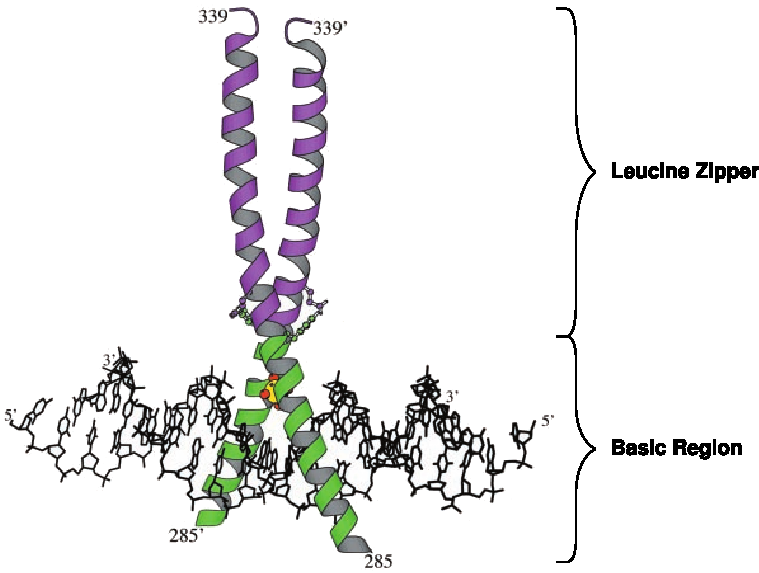
\includegraphics{figuredirectory/bzip.pdf}
\caption{\textbf{Structure of a bZIP transcription factor.} Ribbon
diagram of the cAMP responsive element-binding protein bound to DNA. The
leucine zipper region (purple) mediates the dimerization of the two
monomers. The basic region (green) interacts with the major groove of
DNA (black). Figure modified from Schumacher et al.
(2000)\textsuperscript{306}}\label{figure:2xx:bzip}
\end{figure}

The FD protein is a transcription factor that interacts with both FT and
TFL1 proteins to mediate their association with
DNA\textsuperscript{38,47}. The FD protein contains a basic region
leucine zipper (bZIP) domain, making it a member of the bZIP
transcription factor family\textsuperscript{47}. This family of
transcription factors interact with DNA as dimers (Figure
\ref{figure:2xx:bzip})\textsuperscript{307--309}. The structure of bZIP
transcription factors consists of a basic region that interacts with the
major groove of DNA and mediates the binding of the protein to
transcription factor binding sites\textsuperscript{307,309}. The
dimerization of bZIP monomers is mediated by a coiled-coil structure of
two \(\alpha\)-helicies known as the leucine
zipper\textsuperscript{310}. The coiled-coil structure is stabilized by
hydrophobic amino acid side chains, such as that of leucine, that form a
hydrophobic core to the structure. In addition to the hydrophobic core
of the interaction interface, charged amino acid residues adjacent to
the core influence the binding of monomers through electrostatic
interactions\textsuperscript{307,311}. bZIP transcription factors are
able to form homodimers, a dimer made from two copies of the same
monomer, or heterodimers, where the two monomers are
different\textsuperscript{312}. Indeed, the dimers formed may influence
the genes that will be targeted by the transcription factor, with
dimerization acting as a key regulatory mechanism\textsuperscript{313}.
Changing dimerization and DNA-binding specificity has been found to be
important in the evolution of bZIP transcription factor
function\textsuperscript{314}.

Five of the six copies of \emph{BnFD} expressed in the apex in
\emph{B.~napus} share similar expression profiles (Figure
\ref{figure:230:fdapex}). As a result, it is likely that their protein
products are present in the cell at the same time, and would have the
potential to interact to form dimers. To determine whether the BnFD
proteins are capable of dimerizing, the protein sequences were compared.
Between homologue differences in the protein sequence were identified
between BnFD proteins, with a number of polymorphic sites identified
within the bZIP domain. Amino acid differences observed in the basic
region have the potential to influence DNA binding, while differences in
the leucine zipper region are predicted to influence the dimerization
affinities of the BnFD proteins. The amino acid divergence observed
within the leucine zipper region was also found in bZIP proteins of
other species, suggesting that this form of divergence is frequently
observed among bZIP proteins. Computational modelling of monomer
dimerization suggests that the differences in dimerization affinity
could represent an interesting regulatory mechanism.

\subsubsection{\texorpdfstring{Protein sequence divergence exists
between the six \emph{BnFD}
copies}{Protein sequence divergence exists between the six BnFD copies}}\label{section:spring:bnafddivergence}

\begin{figure}[htbp]
\centering
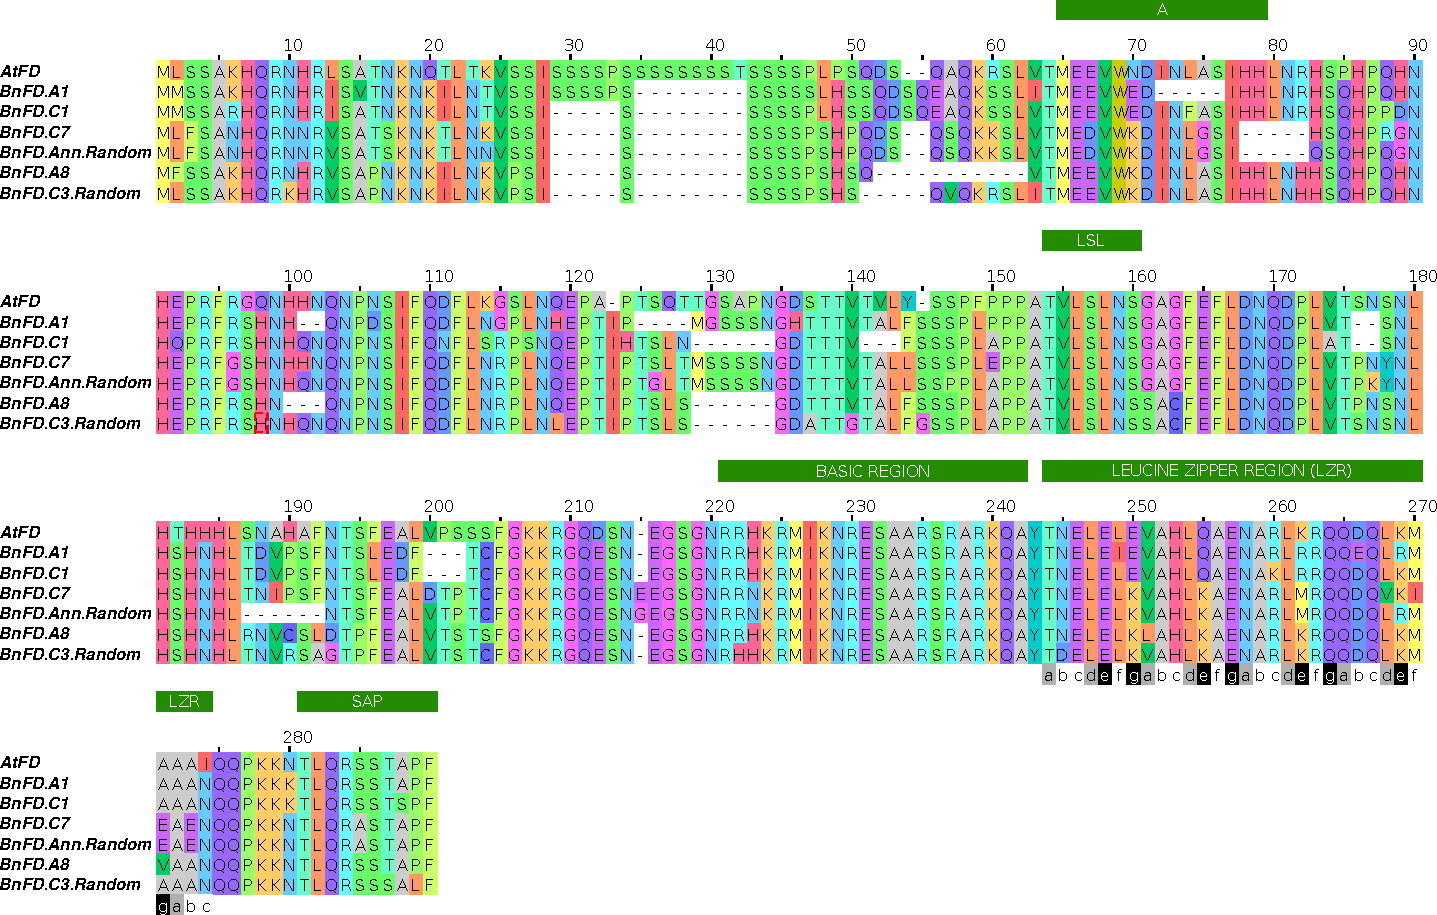
\includegraphics{figuredirectory/34_brassica_sequence_alignment.pdf}
\caption{\textbf{Multiple sequence alignment of the Arabidopsis and BnFD
proteins} The indicated regions of the protein are defined as in Tsuiji
et al. (2013)\textsuperscript{315}. Between copy variation is observed
in the A, BASIC, LEUCINE ZIPPER, and SAP regions. The heptad structure
of the \(\alpha\)-helix that makes up the leucine zipper region is
displayed below the alignment. Amino acid residues located in the
hydrophobic core are residues \texttt{a} and \texttt{d} (black). Amino
acid residues capable of forming electrostatic interactions are in
positions \texttt{e} and \texttt{g} (grey), with between copy variation
visible in these positions.}\label{figure:234:brassicasequence}
\end{figure}

In order to assess the extent of amino acid divergence between the six
copies of \emph{BnFD}, their predicted protein sequences were determined
and aligned (Figure \ref{figure:234:brassicasequence}). To identify
polymorphisms likely to affect the molecular function of the protein,
the results of a comparative study of FD-like genes from many species
were used\textsuperscript{315}. The Arabidopsis FD protein was found to
have four conserved regions: the A region, the LSL region, the bZIP
region (composed of the basic region and a leucine zipper region) and
the SAP region\textsuperscript{315}. Focussing on the same regions in
\emph{B.~napus} (Figure \ref{figure:234:brassicasequence}) identifies a
number of amino acid changes and deletions in the A region, with four
different forms of the region present in the six BnFD proteins.
Comparing the BnFD proteins to the Arabidopsis FD protein reveals that,
in the A region, BnFD.A8 and BnFD.C3 show the greatest amino acid
sequence similarity to the Arabidopsis FD protein, with only a single
amino acid change present.

The LSL region displays no amino acid variation within the
\emph{B.~napus} FD proteins or between species. This is consistent with
the findings of Tsuji et al. (2013), who suggested that the LSL region
was indicative of FD-like proteins that played a role in the floral
pathway\textsuperscript{315}.

In the SAP region, there are again a number of amino acid changes
between the BnFD proteins (Figure \ref{figure:234:brassicasequence}). Of
note is the amino acid polymorphism at position 287 between a theonine
and serine. This position in Arabidopsis becomes phosphorylated and is
important for the binding of FD to the protein FT in Arabidopsis, as
mutation of the threonine to an alanine disrupts complex
formation\textsuperscript{47}. Changing the threonine to a serine was
found to not affect FD binding to FT in Arabidopsis, although
potentially different kinases are responsible for the phosphorylation of
the different residues\textsuperscript{47}.

\subsubsection{Polymorphisms in the DNA binding interface have the
potential to affect binding
affinities}\label{section:spring:fddnabinding}

\begin{figure}[htbp]
\centering
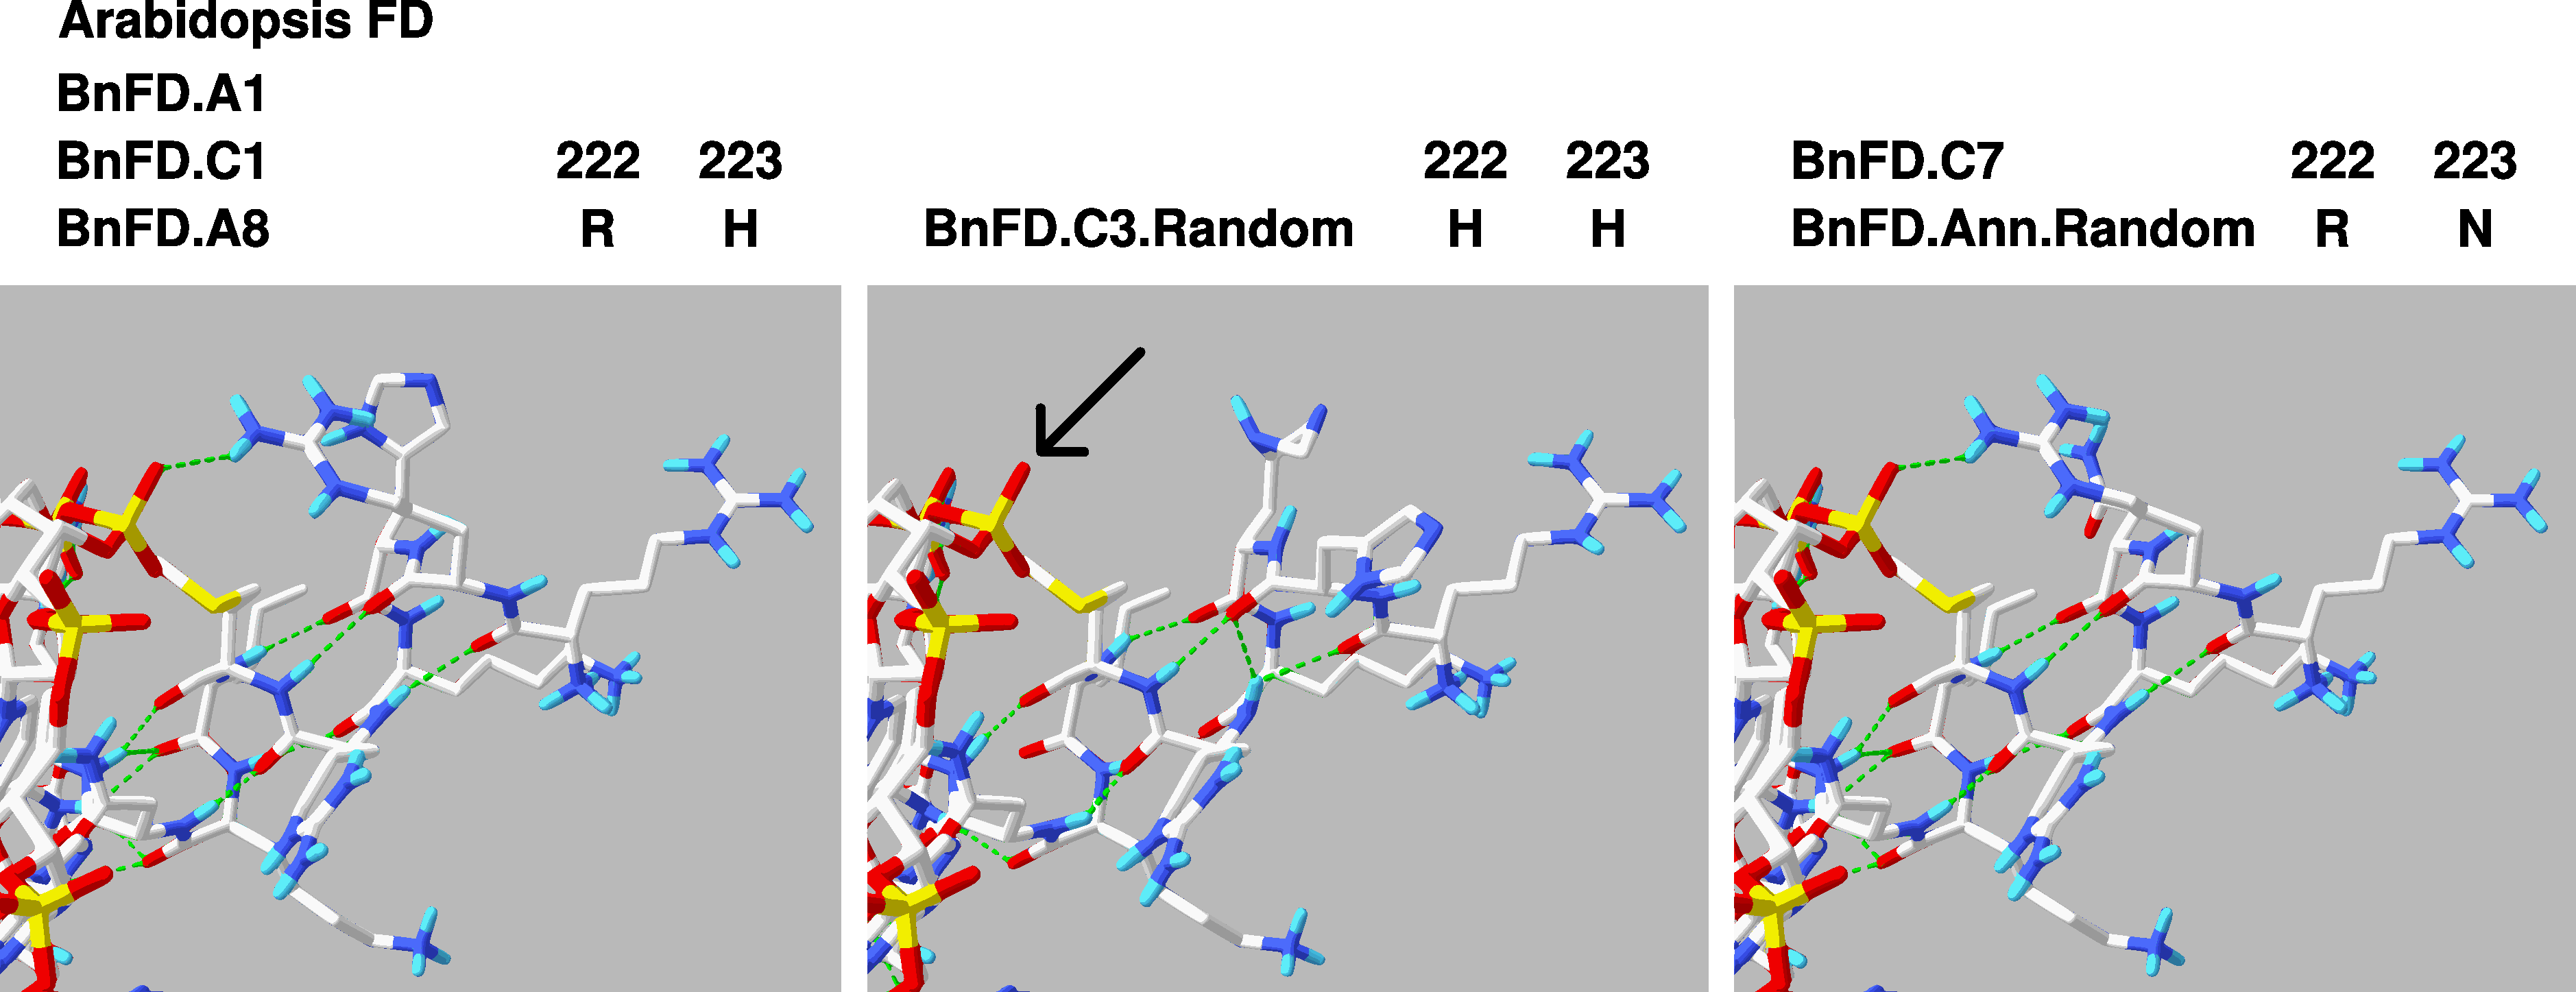
\includegraphics{figuredirectory/35_protein_structure.pdf}
\caption{\textbf{Protein structure of the BnFD proteins complexed with
DNA reveal different hydrogren bonding.} The protein structure of the
CREB protein (PDB ID: 1DH3) from Schumacher et al.
(2000)\textsuperscript{306} was changed to match the amino acids present
in the basic region of BnFD proteins. The single letter codes of the
amino acids replaced, and their positions in the amino acid alignment in
Figure \ref{figure:234:brassicasequence}, are displayed above each plot.
The green dashed lines indicate hydrogen bonding between atoms. The
colour scheme for atoms is as follows: white (carbon), dark blue
(nitrogen), yellow (phosphorus), red (oxygen), and light blue
(hydrogen). Similar hydrogen bonding is observed between the Arabidopsis
FD protein, BnFD.A1, BnFD.C1, BnFD.A8, BnFD.C7, and BnFD.Ann.Random. The
BnFD.C3.Random protein is predicted to lose hydrogren bonding with the
oxygen atom of the DNA backbone indicated with an
arrow.}\label{figure:235:proteinstructure}
\end{figure}

The basic region of bZIP transcription factors forms hydrogen bonds
within the major groove of DNA and consists of the protein-DNA
interaction interface. To investigate whether the amino acid differences
observed in the basic region of the BnFD proteins could impact DNA
binding, predicted hydrogen bonding was analysed. Within the basic
region the BnFD proteins there are two positions that exhibit between
copy differences; positions 222 and 223 (Figure
\ref{figure:234:brassicasequence}). To investigate the potential effects
of these mutations on the DNA binding properties of BnFD, an available
crystal structure of a bZIP transcription factor bound to DNA was used
(PDB ID: 1DH3; Section \ref{sections:methods:fdbinding};
Methods)\textsuperscript{306}. The crystal structure of the mammalian
cAMP responsive element-binding protein (CREB) bZIP transcription factor
bound to DNA revealed that the arginine in position 222 is important as
the amino acid side chain forms a hydrogen bond with the DNA
backbone\textsuperscript{306}. Mapping the amino acids in the basic
region from the BnFD proteins onto the crystal structure of the CREB
transcription factor revealed that changing the amino acid in position
222 from an arginine to a histidine disrupts hydrogen bond formation
between the protein and the DNA (Figure
\ref{figure:235:proteinstructure}). Whether a histidine or an asparagine
is present in position 223 does not seem to affect the hydrogen bonding
in the \(\alpha\)-helix or between the protein and DNA (Figure
\ref{figure:235:proteinstructure}). Therefore, the amino acid
polymorphisms present in the basic region of BnFD proteins potentially
affect the DNA binding affinity of the monomers, but only for the
BnFD.C3.Random protein.

\subsubsection{Amino acid differences in the leucine zipper region of
BnFD proteins is predicted to alter dimerization
affinity}\label{section:spring:fddimerizationprediction}

\begin{figure}[htbp]
\centering
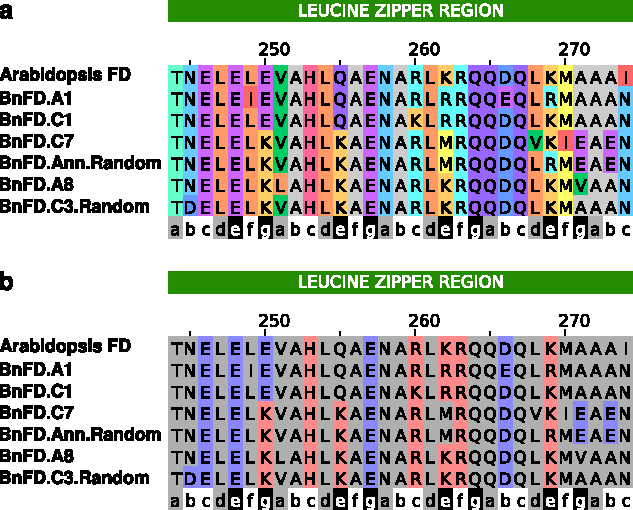
\includegraphics{figuredirectory/brassica_zipper_alignment_with_charges.pdf}
\caption{\textbf{Amino acid differences in the leucine zipper region
result in differently charged amino acids in the \texttt{e} and
\texttt{g} heptad positions.} The amino acid sequence for the
Arabidopsis FD protein and the six \emph{B.~napus} proteins are
displayed. \textbf{a} Amino acids are coloured based on their residue
type. \textbf{b} Amino acids are coloured based on their charge. Blue
coloured amino acids have positively charged side chains while the red
coloured amino acids have negatively charged side
chains.}\label{figure:236a:leucinezipper}
\end{figure}

\begin{figure}[htbp]
\centering
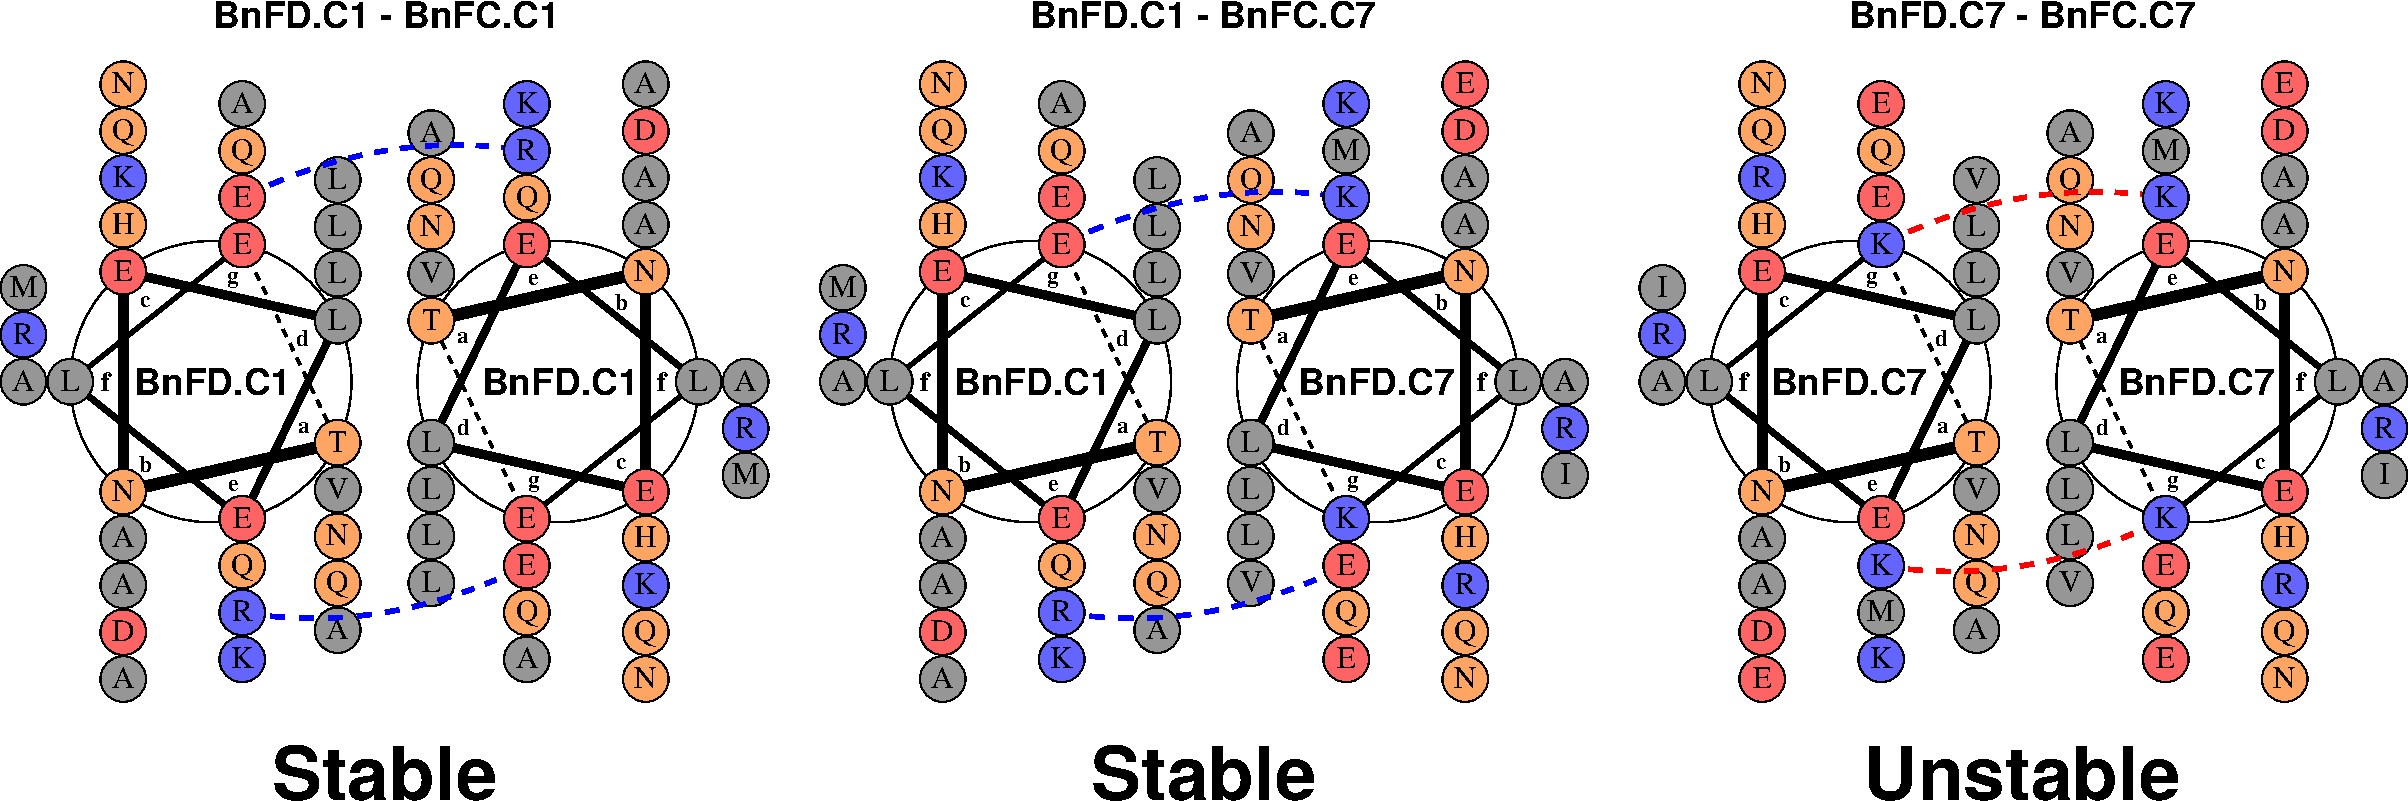
\includegraphics{figuredirectory/36_helical_wheels.pdf}
\caption{\textbf{Helical wheel representation of the homodimers and
heterodimer possible with the \emph{Brassica napus} genes BnFD.C1 and
BnFD.C7 proteins.} The coiled-coil structures of the leucine zippers are
represented as helical wheels. Amino acids in the seven position of the
\(\alpha\)-helix are displayed, with the columns of amino acids
representing the amino acids the entire length of the coiled coil. The
blue coloured amino acids have positively charged side chains, the red
coloured animo acids have negatively charged side chains, and the orange
amino acids have polar side chains. The blue and red dotted lines
between helical wheels indicate attractive and repulsive electrostatic
charges between the two helicies respectively. The helical wheels
demonstrate that attractive forces are predicted to form between the
BnFD.C1 homodimer and the BnFD.C1-BnFD.C7 heterodimer, while a repulsive
force is present in the BnFD.C7 homodimer. The helical wheels were drawn
using DrawCoil\textsuperscript{316} (version
1.0).}\label{figure:236b:helicalwheels}
\end{figure}

Several amino acid differences between the BnFD proteins occur in the
leucine zipper region (Figure \ref{figure:236a:leucinezipper}a). To
determine whether these differences have the potential to alter the
dimerization affinity of the proteins, the amino acid polymorphisms were
assessed in the context of the coiled-coil dimerization interface
(Figure \ref{figure:236b:helicalwheels}). Previous studies of bZIP
transcription factors have revealed that amino acid residues in the
\texttt{e} and \texttt{g} positions of the \(\alpha\)-helix heptad are
important in the determination of dimerization
specificity\textsuperscript{308,311}. Specifically, when the proteins
form a coiled-coil structure, the side chain of an amino acid in the
\texttt{e} position on one \(\alpha\)-helix is able to form
electrostatic bonds with the side chain of an amino acid in the
\texttt{g} position on the other \(\alpha\)-helix (Figure
\ref{figure:236b:helicalwheels}). This is illustrated in the helical
wheel representations in Figure \ref{figure:236b:helicalwheels}, that
represent the positions of amino acids in the coiled-coil. An example of
this is residue 250 (in the \texttt{g} position of the heptad) which has
the capacity to form electrostatic interactions with residue 255 (in the
\texttt{e} position of the heptad; Figure
\ref{figure:236a:leucinezipper}a) due to their opposing charges.
Therefore, the charge these residues carry is a factor which determines
the dimerization affinity between bZIP proteins. Positions 250, 255, 262
and 271 are all in either the \texttt{e} or \texttt{g} positions of the
heptads and show amino acid polymorphisms which alter the charge of the
amino acid side chains (Figure \ref{figure:236a:leucinezipper}b). The
effect this has on the predicted electrostatic interactions is
illustrated in Figure \ref{figure:236b:helicalwheels}. The BnFD.C1
homodimer and the BnFD.C1-BnFD.C7 heterodimer are both predicted to have
attractive electrostatic interactions between the two monomers, while a
repulsive force is predicted for the BnFD.C7 homodimer (Figure
\ref{figure:236b:helicalwheels}). These polymorphisms suggest that
certain dimer combinations of the BnFD proteins will be more favoured
than others.

\begin{figure}[htbp]
\centering
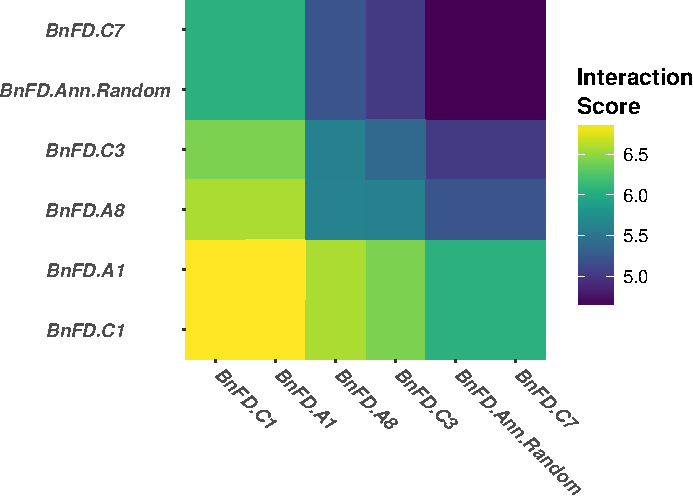
\includegraphics{figuredirectory/37_fd_dimer_heatmap.pdf}
\caption{\textbf{Heatmap of the dimerization affinity scores computed
between BnFD leucine zipper regions.} The machine learning algorithm
developed by Potapov et al. (2015)\textsuperscript{317} was used to
score the dimerization affinity of the leucine zipper regions of the
possible BnFD dimers. Higher scoring dimers are more likely to form than
lower scoring dimers. The leucine zipper regions used for the analysis
correspond to the region indicated in Figure
\ref{figure:236a:leucinezipper}a. The heatmap reveals that certain BnFD
dimers are predicted to be more likely to occur than
others.}\label{figure:237:bnafdheatmap}
\end{figure}

The sequence analysis suggests that the amino acid polymorphisms
observed in the \texttt{e} and \texttt{g} positions of the heptad may
affect the dimerization affinity of the proteins. To investigate this in
a more quantitative manner, a published machine learning
algorithm\textsuperscript{317} was used to score the potential
interaction affinity of pairs of BnFD monomers (Figure
\ref{figure:237:bnafdheatmap}). The interaction scores between the BnFD
monomers range from 4.3 to 7.2, with the higher interaction scores
indicating a higher likelihood of interaction. To put these scores into
context, the dimerization of the bZIP transcription factors Fos and Jun
have been extensively studied in terms of their dimerization
affinity\textsuperscript{311}. It has been shown that the Fos-Jun
heterodimer is more thermally stable than either the Fos homodimer or
the Jun homodimer, with the Fos homodimer being particularly
unfavourable\textsuperscript{311}. Using the machine learning scoring
algorithm of Potapov et al. (2015)\textsuperscript{317}, Fos homodimers
score 6.2, Jun homodimers score 6.3 and Fos-Jun heterodimers score 8.8.
The score range for Fos and Jun dimers is 2.6, a similar range as that
observed for the BnFD proteins. Therefore, the differences in
interactions scores observed between the BnFD proteins are large enough
to suggest a functional effect. The interaction scores group the six
BnFD genes into three interaction groups (Figure
\ref{figure:237:bnafdheatmap}). BnFD.C1 and BnFD.A1 form a group which
have a higher affinity for forming dimers between themselves than with
the remaining four proteins. BnFD.A8 and BnFD.C3.Random are more likely
to form dimers with both BnFD.C1 and BnFD.A1 rather than themselves.
Finally, BnFD.Ann.Random and BnFD.C7 have the lowest likelihood to form
dimers between themselves relative to the other dimers tested, and have
the highest likelihood to form dimers with both BnFD.C1 and BnFD.A1. The
machine learning approach predicts that the six copies of BnFD have
variation in their dimerization affinities, with four of the six copies
predicted to form more stable heterodimers than homodimers. The range of
interaction scores predicted for the BnFD proteins is similar in size to
the range of interaction scores predicted for the Fos and Jun proteins,
suggesting that the predicted differences have the potential to be
biologically relevant.

\subsubsection{Changes in dimerization affinities may be a common way of
bZIP proteins
diverging}\label{changes-in-dimerization-affinities-may-be-a-common-way-of-bzip-proteins-diverging}

\begin{figure}[htbp]
\centering
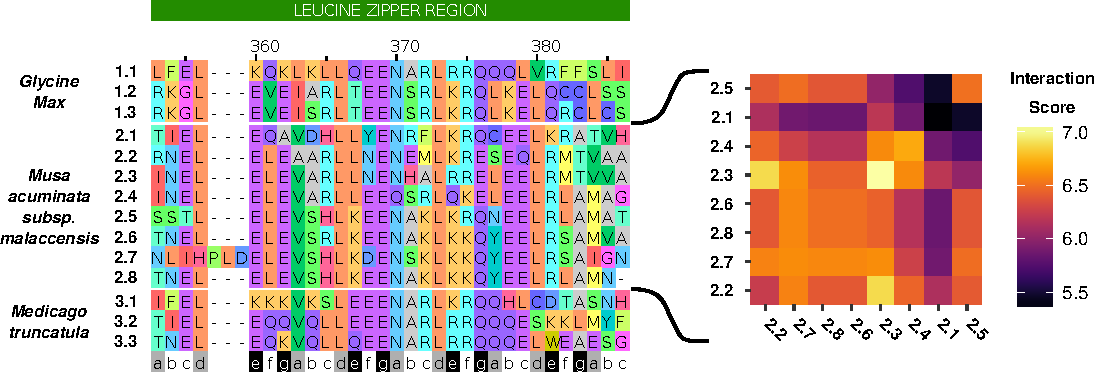
\includegraphics{figuredirectory/38_ensembl_with_heatmap.pdf}
\caption{\textbf{Multiple sequence alignment of the leucine zipper
region of Arabidopsis \emph{FD} orthologues in \emph{Glycine max},
\emph{Musa acuminata subsp. malaccensis}, and \emph{Medicago
truncatula}.} Amino acids are coloured based on their residue type.
Several amino acid differences resulting in side chain charge
differences are observed in the \texttt{e} and \texttt{g} heptad
positions. The effect these changes have on the interaction scores
calculated using the method of Potapov et al.
(2015)\textsuperscript{317} are displayed as a heatmap for the
\emph{M.~acuminata} orthologues. The gene names are displayed in Table
\ref{appendix:figure238table}; Appendix A.}\label{figure:238:ensembl}
\end{figure}

\begin{figure}[htbp]
\centering
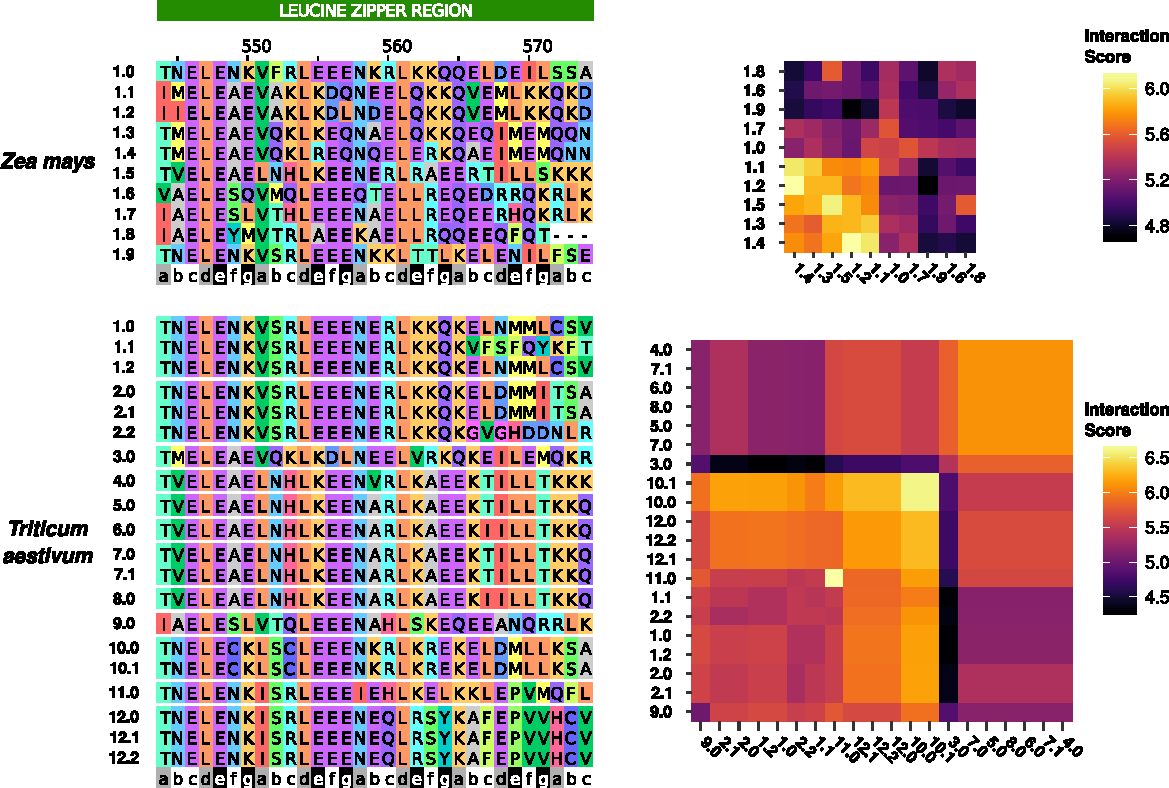
\includegraphics{figuredirectory/39_brassica_wheat_maize_fd.pdf}
\caption{\textbf{Multiple sequence alignment of the leucine zipper
regions of the proteins with highest amino acid similarity to
Arabidopsis FD from the \emph{Zea mays} and \emph{Triticum aestivum}
proteomes.} Amino acids are coloured based on their residue type.
Several amino acid differences resulting in side chain charge
differences are observed in the \texttt{e} and \texttt{g} heptad
positions. The effect these changes have on the interaction scores
calculated using the method of Potapov et al.
(2015)\textsuperscript{317} are displayed as heatmaps. The \emph{Z.
mays} proteins plotted were chosen by selecting the \emph{Z. mays}
protein with the highest sequence similarity to the AtFD protein and
then including the paralogues of the gene as identified in the
EnsemblPlants database\textsuperscript{318}. The \emph{T. aestivum}
proteins were identified in the same way, except that in addition to the
paralogues, the homoeologues of all proteins were also included. The
gene names are displayed in Table \ref{appendix:figure239wheatmaizefd};
Appendix A.}\label{figure:239:wheatmaizefd}
\end{figure}

To investigate whether polymorphisms influencing dimerization affinity
were a common occurrence in organisms where gene multiplication events
have occurred, sequences of \emph{FD} orthologues identified in the
EnsemblPlants database\textsuperscript{318} were aligned. Only those
species containing multiple Arabidopsis \emph{FD} orthologues in the
genome are displayed in Figure \ref{figure:238:ensembl}. Focussing on
the leucine zipper regions of these proteins reveals similar charge
influencing polymorphisms in the \texttt{e} and \texttt{g} heptad
positions between the genes within a species. Charge influencing
polymorphisms in the \texttt{e} and \texttt{g} heptad positions are
present in the \emph{Glycine max} orthologues at positions 360, 362 and
381, \emph{Musa acuminata} at positions 362, 367, 374 and 376 and
\emph{Medicago truncatula} at positions 360, 362, 367 and 381. Likewise,
\emph{Zea mays} and \emph{Triticum aestivum} proteins with high sequence
similarity to Arabidopsis \emph{FD} also exhibit polymorphisms in the
\texttt{e} and \texttt{g} heptad positions that alter the charge of the
amino acid side chain. The machine learning
algorithm\textsuperscript{317} predicts considerable variation in the
dimerization affinity for the identified FD-like proteins, with the
range of scores being similar to the range identified for the BnFD
proteins. These findings suggest that variation in dimerization
affinities between duplicated bZIP proteins is frequently observed in
different plant species.

\subsubsection{Variation in dimerization affinity influences the
proportions of hetero- and homodimers expected at steady
state}\label{variation-in-dimerization-affinity-influences-the-proportions-of-hetero--and-homodimers-expected-at-steady-state}

\begin{figure}[htbp]
\centering
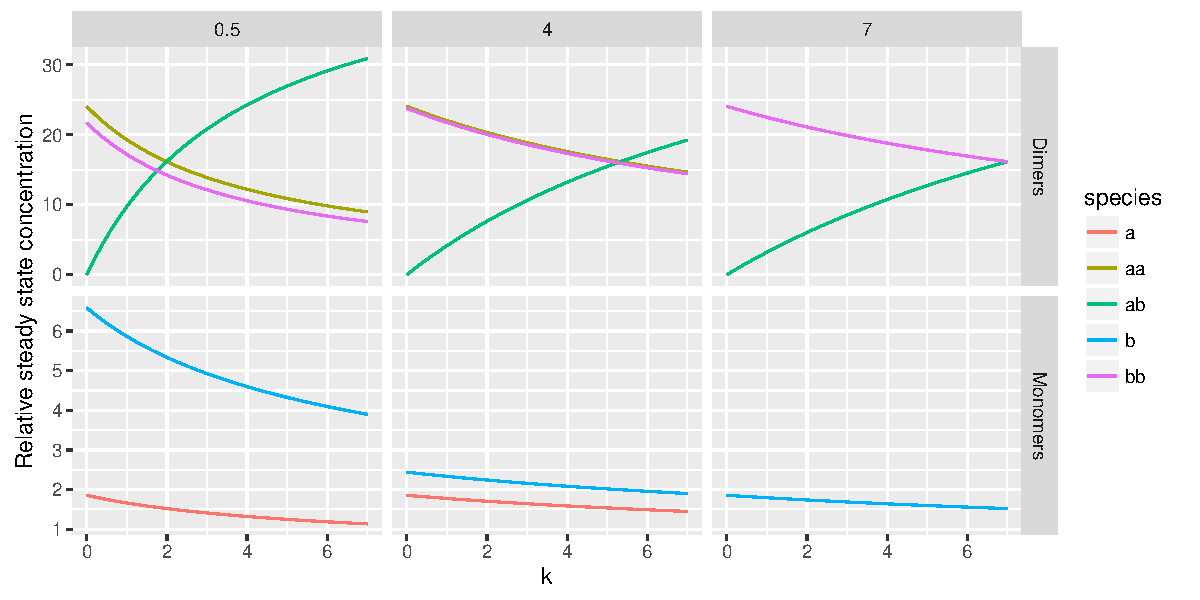
\includegraphics{figuredirectory/40_fd_dimerization.pdf}
\caption{\textbf{Dimerization affinity differences influence the dimer
population expected at steady state.} The steady state concentrations of
monomers and dimers are displayed. The simulation was run with different
\texttt{bb} homodimer production rate, either 0.5 (\textbf{a}), 4.0
(\textbf{b}), or 7.0 (\textbf{c}), and was started with equal
concentrations of each monomer. The equilibria simulated, with the rate
constants used, are displayed below the plot. The x-axis corresponds to
the \texttt{ab} heterodimer production rate. To generate these results
the system of equations were modelled as ordinary differential equations
and numerically solved. The concentrations plotted are steady state
concentrations of the system. The simulations reveal that as the
dimerization affinity of the \texttt{bb} dimer decreases, the relative
concentrations of the \texttt{ab} heterodimer and \texttt{b} monomer at
steady state increase. The simulations were run as described in Section
\ref{sections:methods:fdmodelling};
Methods.}\label{figure:240:dimerizationmodelling}
\end{figure}

To test potential regulatory repercussions of altered dimerization, a
system of ordinary differential equations was used to model the
dimerization reactions. Two different monomer types, \texttt{a} and
\texttt{b}, were modelled, with the monomers able to form homodimers
(\texttt{aa} and \texttt{bb}) and a heterodimer (\texttt{ab}). To
investigate how the behaviour of the system depends on the dimerization
affinities, three different reaction rates for the homodimerization of
the \texttt{b} species were tested; 0.5, 4.0 and 7.0. For each of these
rates, the heterodimerization rate for the monomers was varied and the
steady state concentrations of the various species calculated. Equal
concentrations of each monomer were used as the initial conditions of
the model, and the system of equations was numerically solved until a
steady state was reached (Figure \ref{figure:240:dimerizationmodelling};
Section \ref{sections:methods:fdmodelling}; Methods). When all
dimerization rates are 7.0, the steady state concentrations of all
dimers are identical (Figure \ref{figure:240:dimerizationmodelling}c)
For a \texttt{b} homodimerization rate of 7.0, the two homodimer species
have the same steady state concentrations at all heterodimerization
rates, as expected given that all dimerization reactions have the same
reaction rates. By setting the \texttt{b} homodimerization rate to 0.5,
the \texttt{bb} homodimer is disfavoured, with an observed increase in
the steady state concentration of the undimerizaed \texttt{b} monomer.
This also affects with the steady state concentration of the
heterodimer. Above a heterodimer formation rate of \textasciitilde{}2.0,
the heterodimer becomes more favourable than either of the homodimers.
The simulation results reveal that an unfavourable \texttt{bb} homodimer
increases the \texttt{b} monomer concentration at steady state. A high
relative concentration of the \texttt{b} monomer favours the formation
of the \texttt{ab} heterodimer rather than the \texttt{aa} homodimer.
This is despite the forward reaction rate of the \texttt{aa} homodimer
being 2.5 times greater than the \texttt{ab} heterodimer formation rate.
A similar pattern is observed when less extreme \texttt{bb} homodimer
formation rate of 4.0 is used in the modelling.

\subsection{Conclusions}\label{conclusions-3}

Analysing sequence divergence between \emph{B.~napus} homologues of two
Arabidopsis floral integrators highlights the potential role both
cis-regulatory elements and non-synonymous sequence differences play in
gene divergence following duplication. The expression divergence
observed between \emph{BnTFL1} genes in the transcriptomic time series
suggested that cis-regulatory element changes may have occurred.
Comparing the downstream sequence of \emph{BnTFL1} genes with
Arabidopsis \emph{TFL1} identified different patterns of sequence
conservation for different homologues. These regions of differential
sequence conservation were located in regions previously shown in
Arabidopsis to contain cis-regulatory elements\textsuperscript{303}.
\emph{TFL1} expression dynamics in Arabidopsis mutants lacking these
cis-regulatory elements\textsuperscript{303} were consistent with the
expression of \emph{BnTFL1} genes lacking sequence conservation within
those elements. A region II was found to be important for \emph{TFL1}
upregulation in the meristem during the floral
transition\textsuperscript{303}. The genes observed to increase during
the floral transition, \emph{BnTFL1.A10} and \emph{BnTFL1.C3}, exhibit
sequence conservation within region II, while genes that do not exhibit
an increase during the floral transition, \emph{BnTFL1.C2} and
\emph{BnTFL1.Cnn.Random}, do not. This conservation suggests that the
spatiotemporal domains of expression defined by the cis-regulatory
elements is conserved between \emph{B.~napus} and Arabidopsis. Although
the relationship between the sequence conservation downstream of the
\emph{BnTFL1} genes and the expression profiles exhibited by the genes
is correlative, it provides a hypothesis to be tested by future studies.
This case study is potentially an example of cis-regulatory element
changes driving the development of novel gene functions, as predicted by
the DDC model\textsuperscript{209}.

For the \emph{BnFD} genes, expression profiles suggest that five of the
six genes are co-regulated and potentially form dimers amongst
themselves\textsuperscript{47,307}. To investigate whether the different
copies of the gene could potentially dimerize, the protein sequences of
the genes were analysed. Amino acid differences were observed in
multiple domains identified as conserved in FD-like proteins from
diverse plant speciea\textsuperscript{315}. An amino acid change in the
SAP domain in the BnFD.C3.Random protein corresponds to an amino acid
that is important for the interaction of the protein with
FT\textsuperscript{47}, suggesting this copy may have altered protein
binding. Amino acid differences identified in the DNA binding basic
region, when compared to published crystal structures of bZIP
transcription factors\textsuperscript{306}, suggest that the
BnFD.C3.Random protein may also exhibit altered DNA binding. However,
without characterising this experimentally, it is difficult to determine
whether the single amino acid changes observed would have an appreciable
effect on DNA binding. A potential improvement on the analysis presented
here would be to perform more accurate predictions of hydrogen bond
formation\textsuperscript{319,320}. Between homologue amino acid
differences in the leucine zipper region were predicted to alter the
dimerization dynamics between BnFD proteins, with certain dimers
predicted to be more likely to occur than others. Investigating
\emph{FD} orthologues in other species revealed that variation in
dimerization affinity might be a common form of divergence for bZIP
transcription factors that are present as multiple copies in the genome.
Computational modelling of the dimerization dynamics suggest that having
a system of monomers with different dimerization affinities can result
in interesting regulatory consequences. However, this is dependent on
the dimers formed having different molecular activities.

\section{Discussion}\label{discussion}

Polyploidy plays a large factor in the success of both
domesticated\textsuperscript{321}, and wild\textsuperscript{322} plants.
The gene duplication following whole genome duplication introduces a
vast amount of genetic material. The relaxed selective pressures allow
for duplicated genes to acquire new roles, neofunctionalize, become more
specialized, subfunctionalize, or be lost or silenced, the latter being
the most common outcome for duplicated genes\textsuperscript{208}.
Despite this, a significant number of genes have been observed to be
retained following gene duplication\textsuperscript{293}. This has led
to the gene dosage hypothesis being proposed, which states that dosage
sensitive genes are preferentially retained in the genome following
whole genome duplication to maintain the stoichiometry of protein
complexes\textsuperscript{220,223}. This has been observed in
Arabidopsis, with signal transduction and transcription factors being
preferentially retained\textsuperscript{293} in the Arabidopsis genome
following whole genome duplication\textsuperscript{10,323,324}.

To investigate the factors influencing gene retention in
\emph{B.~napus}, particularly for the flowering time genes, a
transcriptomic time series was developed for \emph{B.~napus}. The time
series spanned from early growth to flower development, to allow
transcriptomic changes during the floral transition to be followed. In
order to confirm that the transcriptomic time series was able to capture
biologically relevant effects, GO term and protein domain enrichment was
performed. GO term analysis revealed transcriptional responses
appropriate to the tissue. For example, genes associated with leaf
senescence were upregulated in the leaf towards the end of the time
series and genes associated with the regulation of flower development
responding as expected in the apex (Figure \ref{figure:219:go1som}). The
response of the circadian rhythm genes to the vernalization period in
both the leaf and apex revealed that the short day conditions of the
cold treatment were influencing transcription (Figure
\ref{figure:221:go3som}). The sessile nature of plants means that they
need to interpret environmental signals and alter their development
accordingly. As such, the circadian clock in plants becomes entrained to
different light regimes\textsuperscript{16}, and this effect is likely
responsible for the response here. That genes associated with the
circadian rhythm respond during the cold treatment needs to be taken
into account when considering the expression profiles of other genes in
the transcriptomic time series.

\subsection{Gene retention}\label{gene-retention}

Genome dominance, that is, the finding that gene expression is biased
towards different gene copies from one genome, is a potential method by
which gene expression can diverge\textsuperscript{285,286}. The results
from the transcriptomic time series reveal that if all genes are
considered, the A genome tends to have a higher proportion of genes that
are highly expressed whereas the C genome as a higher proportion of
lowly expressed genes. Interestingly, this pattern is not observed when
pairs of homoeologues are considered, with a greater number of pairs
exhibiting bias towards the C genome. This was found to occur
independent of tissue, in contrast to previous results in
\emph{B.~napus} that suggested genome dominance may be tissue and
developmental time specific\textsuperscript{325}. While the results from
the genome level and homoeologue level analysis may initially seem
contradictory, observations in maize suggest that gene loss is biased
towards the genome that has reduced homoeologue
expression\textsuperscript{287}. Therefore, gene loss may have occurred
more frequently on the A genome, leading to the proportionally higher
expression when all genes are considered. The potential effect of genome
biased expression, however, is uncertain. In \emph{Coffea arabica},
differential use of homoeologues was not found to contribute to the
ability of plants to tolerate a broader range of growing temperatures
than its diploid parents\textsuperscript{326}. However, in
\emph{Gossypium hirsutum} differential homoeologue expression was found
to be tissue specific\textsuperscript{285}, suggesting the copies are
functionally distinct. The age of the polyploid likely plays a
significant role in this, with biased expression being observed more
frequently in recent or synthesised allopolyploids rather than natural
polyploids\textsuperscript{282,327}. As the polyploidy event leading to
\emph{B.~napus} occurred less than 10,000 years
ago\textsuperscript{103}, relative to the 1~-~2 million years of
cottom\textsuperscript{327}, or the 5~-~12 million years of
maize\textsuperscript{287}, potentially the homologue differences
observed are a consequence of \emph{B.~napus} being a relatively young
polyploid.

Investigating the subset of flowering time genes in \emph{B.~napus}
reveals that these genes seem to be preferentially retained relative to
the entire genome. Similar patterns are also observed when just
expressed genes are considered, suggesting that the additional copies of
flowering time genes are expressed and functional. Given that the
majority of flowering time genes are transcription factors, that are
involved in highly networked gene regulatory
networks\textsuperscript{101,288}, the gene dosage theory predicts their
retention in the genome\textsuperscript{220,223}. The gene dosage
hypothesis predicts that genes that are dosage sensitive will tend to be
retained in the genome. However, differences in the number of expressed
versus annotated genes, the WGCNA-based clustering, and the SOM-based
clustering, all suggest that expression divergence between copies is
common. For flowering time genes, 61~\% and 69~\% of Arabidopsis genes
in the apex and leaf, respectively, have at least one \emph{B. napus}
gene that lacks expression in the time series. This potentially suggests
that these genes are part of responsive backup
circuits\textsuperscript{215,216}. A prediction from this observation,
assuming these genes are part of such backup circuits, is that these
copies that are not expressed would be expressed if one of the other
expressed copies became silenced\textsuperscript{215,216}. A potential
method of testing this would be to leverage the variation present among
different \emph{B.~napus} varieties\textsuperscript{328}, to identify if
homologue preference is observed. The alternative possibility is that
the homologues exhibit tissue specific expression\textsuperscript{285},
and that this is not captured in the leaf or apex transcriptomes.
Determining the expression of these homologues in other tissues besides
the apex and leaf would allow this to be tested.

To determine divergence among expressed genes, two clustering approaches
were employed. The WGCNA-based clustering approach revealed that, both
genome wide and among flowering time genes, that expressed homologues
have diverged in terms of their expression profiles across the
transcriptomic time series. These results were supported by the
SOM-based approach, that was used to ensure the observed divergence was
robust to the uncertainty inherent in gene expression data. This
suggests that evolutionary mechanisms other than gene dosage have played
a role in the retention of flowering time genes in the \emph{B.~napus}
genome. This is consistent with observations in Arabidopsis that
revealed 85~\% of paralogous regulatory genes exhibit expression that
suggests neo- or subfunctionalization\textsuperscript{329}. The
divergence of expression patterns can be explained by both the DDC and
the escape from adaptive conflict hypotheses\textsuperscript{209,212}.
The former hypothesis would predict that deleterious mutations have
arisen in cis-regulatory elements, resulting in divergent expression
patterns. The escape from adaptive conflict hypothesis posits that the
different expression patterns of the genes may represent an adaptive
partitioning of ancestral gene function. Either way, both of these
potential hypotheses suggest that changes to cis-regulatory elements or
to other regulatory machinery post-duplication. These findings for
\emph{B.~napus} genes are consistent with findings that suggests
regulatory divergence is one of the primary mechanisms by which genes
diverge after a duplication\textsuperscript{330}.

The flowering time genes were the focus of this work, and this was aided
by curated lists of flowering time genes being
available\textsuperscript{288}. However, the patterns observed at the
whole genome level suggest that homologue divergence is relatively
common, with 69~\% and 62~\% of Arabidopsis genes in the apex and leaf
respectively having at least one \emph{B.~napus} homologue located in a
different regulatory module. An interesting avenue for future work would
be to determine other subsets of genes that seem to be preferentially
retained in the genome and determine whether similar expression
divergence is observed. Good candidates for such groups of genes would
be genes whose products are involved in signal transduction pathways, as
these were found to be preferentially retained in
Arabidopsis\textsuperscript{293}.

Although regulatory divergence between homologues is observed for the
majority of Arabidopsis genes, many homologues do still exhibit similar
expression profiles. The similarity of homoeologue expression patterns
among flowering time genes revealed that many are found in the same
regulatory module (79~\% in the apex and 77~\% in the leaf). Similarity
in the expression of some homologues is also observed at the genome wide
level, represented in the WGCNA-based analysis as groups of homologues
occupying fewer regulatory clusters than the number of homologues
present (Figure \ref{figure:215:wgcnaall}). At the individual gene
level, the \emph{BnLFY} genes all exhibit similar expression profiles,
which is interesting given the dosage sensitivity of the \emph{LFY} gene
in Arabidopsis\textsuperscript{69,70}. Homologues exhibiting similar
expression profiles could represent genes where gene dosage based
selection is maintaining them in the genome. However, due to the
relatively young age of \emph{B.~napus} as a
polyploid\textsuperscript{103} it is also possible that these genes are
redundant and selective pressures have not yet removed the duplicate
copies from the genome, as theory would
predict\textsuperscript{208,211}. An important determinant of whether
genetic redundancy is stable in the genome, and how long redundant genes
are maintained in the genome if it is not stable, is the mutational rate
of the duplicated genes\textsuperscript{211}. Although mutational rates
have been determined in other organisms\textsuperscript{331,332}, no
such data is available for \emph{B. napus}. If such data were available
for \emph{B. napus}, it would strengthen conclusions about whether
seemingly redundant genes are in a transient state before being lost
from the genome or whether redundancy is being selected for. As
additional aspect of this would be the effect artificial selection and
breeding has had on the retention of duplicate genes. Mutational rates
can be artificially altered to introduce variation into breeding
genotypes\textsuperscript{333}, and potentially in this scenario of high
mutational rates selection for genes that are redundant is favoured.

\subsection{Floral transition}\label{floral-transition}

The floral transition is one of the most important developmental
transitions an angiosperm can go through. Floral integrators form a
tightly interconnected gene regulatory network that ensures the timing
of the floral transition is consistent\textsuperscript{288}. Indeed, the
structure of this network confers favourable behaviours such as noise
filtering of input signals and irreversability\textsuperscript{38}. To
determine whether this network is conserved in \emph{B.~napus}, the
expression profiles of the key floral integrator genes were
investigated. The tissue specificity of expression, and the expression
profiles themselves, were generally consistent with the expression of
the genes in Arabidopsis. At least one \emph{B.~napus} homologue
displays an expression profile consistent with that expected from
Arabidopsis. This suggests a general conservation between the regulatory
network underlying flowering in Arabidopsis and \emph{B. napus}, that
will aid efforts to translate knowledge from Arabidopsis to the crop.

Of the floral integrators, \emph{BnFT} is the most well studied,
potentially because of its proximity to regions of the genome found to
be associated with flowering time\textsuperscript{131,298}. All four
profiles are upregulated after the cold period, as expected from
Arabidopsis\textsuperscript{20--22}. The A7 and C6 copies were found to
exhibit divergence relative to the A2 and C2 copies. In the leaf these
copies exhibit a greater fold different between pre-cold expression
levels and post-cold peak expression levels. This is interesting given
results from vernalization sensitive lines of \emph{B. napus} that found
the A7 and C6 copies were silenced prior to vernalization, whereas the
A2 copy was expressed prior to vernalization\textsuperscript{150}.
Although Westar is a spring variety, a slight vernalization response is
still observed and \emph{BnFLC} genes in the variety display expression
consistent with being vernalization sensitive\textsuperscript{234}
(section \ref{section:winter:flc}). This potentially suggests that these
copies mediate are vernalization responsive in Westar. However, this
response may be variety specific, as other findings from Guo et al.
(2014)\textsuperscript{149} found \emph{BnFT.A7} and \emph{BnFT.C6} to
be most highly expressed when floral buds were visible, which does not
agree with results from the transcriptomic time series. It is also
interesting that \emph{BnFT.C2.Random} is found to exhibit expression,
given that multiple accounts have reported that the C2 copy of
\emph{BnFT} is not expressed\textsuperscript{149,150}. This could
represent a difference between spring and winter varieties of
\emph{B.~napus}. The expression of \emph{BnFT.A7} and \emph{BnFT.C6} in
the apex is somewhat surprising, given that \emph{FT} in Arabidopsis is
not required for the function of the gene to promote
flowering\textsuperscript{22,42,47}. Although \emph{FT} homologues are
expressed in the apex in cabbage
(\emph{B.~oleracea})\textsuperscript{140}, and seem to be involved with
the floral transition in the plant, the morphological differences
between cabbage and oilseed rape make the findings difficult to compare.
Finally, the expression profiles of \emph{BnFT} copies in the leaf
suggest that the experimental design decision to subject the spring
variety to the same vernalization treatment of the winter variety likely
aided in synchronizing the development of the two varieties. The high
expression of \emph{BnFT} genes prior to the cold suggests that the
Westar plants were capable of flowering prior to the cold treatment, as
would be expected of a spring variety. The short day photoperiod of the
vernalization treatment seemingly repressed \emph{FT} expression until
after the cold, delaying the flowering of the spring
variety\textsuperscript{296}.

For the other floral integrators, less is known about their expression
in \emph{B.~napus}. However, the expression profiles of all \emph{BnLFY}
genes, and the most highly expressed \emph{BnAP1} genes, are fully
consistent with the roles the homologous genes have in
Arabidopsis\textsuperscript{72,78}. The \emph{BnSOC1} genes exhibit
spatial divergence, with \emph{BnSOC1.A3.Random} and \emph{BnSOC1.A5}
most highly expressed in the apex and \emph{BnSOC1.A4} and
\emph{BnSOC1.C4.Random} most highly expressed in the leaf. This suggests
that these copies may have undergone spatial
subfunctionalization\textsuperscript{202,209}. Further divergence is
observed between the \emph{BnSOC1} expression profiles, with some copies
responding to vernalization, while others do not. This suggests that
different \emph{BnSOC1} genes have diverged to respond to different
inputs. In Arabidopsis \emph{SOC1} is downstream of the FT protein,
becoming upregulated in the apex when \emph{FT} is
expressed\textsuperscript{20,46,82,301,302}. The only copy consistent
with this regulatory interaction in the apex is \emph{BnSOC1.A3.Random},
making it a good candidate for maintaining the same role as \emph{SOC1}
in Arabidopsis. For the copies that exhibit expression consistent with
Arabidopsis, a similar approach to the one taken by Tadege et al.
(2001)\textsuperscript{141} could be employed, with the best candidates
transformed into Arabidopsis mutants to determine whether they indeed
retain their role or not.

Despite the similarities between the regulation of Arabidopsis and
\emph{B.~napus} floral genes, divergence is observed between
\emph{B.~napus} homologues of floral genes. In Arabidopsis, duplicated
regulatory networks have been observed to diverge, such that parallel
networks that are spatiotemporally distinct are
formed\textsuperscript{293}. If this was the case with the gene
regulatory network underlying flowering in \emph{B.~napus}, divergence
would be expected for all floral integrators. However, the analysis here
reveals that \emph{B. napus} homologues of floral integrators instead
exhibit different patterns of regulatory module assignment. At one
extreme \emph{BnLFY} genes seem not to have diverged relative to each
other in terms of expression profile, while at the other extreme all
four copies of \emph{BnTFL1} exhibit different expression profiles. This
suggests that the gene regulatory network underlying flowering has not
diverged to form parallel networks in \emph{B. napus}. This is
potentially due to differences in the evolutionary time that has elapsed
since gene duplication. The gene duplication analysed in the Arabidopsis
genome, that lead to the observed formation of parallel networks,
occurred 20~-~60 million years ago\textsuperscript{208,293,334}.
However, the genome triplication to give the ancestral hexaploid
\emph{Brassica} ancestor occurred 8~-~23 million years
ago\textsuperscript{108,109}, while the interspecies hybridization event
to give \emph{B.~napus} occurred less than 10,000 years
ago\textsuperscript{103}. Therefore, potentially not enough evolutionary
time has elapsed for this form of divergence to be observed.

\emph{BnTFL1} was the only floral integrator where all copies exhibited
expression profiles that are completely divergent. To investigate
potential explanations for this, the regulatory regions surrounding the
gene were investigated. For each \emph{BnTFL1} gene, different patterns
of sequence conservation were observed downstream of the gene, with the
differences correlating with the expression divergence observed between
the genes. This is in agreement with previous investigations of
\emph{BnTFL1} genes, that found between copy sequence conservation both
within the first intron and downstream of the gene\textsuperscript{148}.
Serrano-Mislata et al. (2016) identified and characterised
cis-regulatory elements downstream of the \emph{TFL1} gene in
Arabidopsis\textsuperscript{303}, that colocalized with the regions
displaying sequence conservation differences between \emph{BnTFL1}
genes. The expression of \emph{TFL1} in Arabidopsis mutants lacking
certain cis-regulatory regions\textsuperscript{303} were strikingly
similar to the expression profiles of \emph{BnTFL1} in the
transcriptomic time series. For example, region II (Figure
\ref{figure:233:tfl1conservation}), was identified as important for the
upregulation for \emph{TFL1} in the Arabidopsis apex during the floral
transition\textsuperscript{303}. \emph{BnTFL1} genes lacking sequence
conservation in that region were not upregulated during flowering,
whereas \emph{BnTFL1.C3} and \emph{BnTFL1.A10} which exhibited
conservation in region II were upregulated. Although correlative, these
findings certainly provide hypotheses for future investigations. The
\emph{BnTFL1.Cnn.Random} copy does not exhibit conservation in region
III, identified as responsible for expression of \emph{TFL1} in
Arabidopsis lateral meristems\textsuperscript{303}. Determining whether
this copy is indeed lacking expression in the lateral meristem would be
one way of testing whether the cis-regulatory elements downstream of
\emph{TFL1} genes are conserved between \emph{B.~napus} and Arabidopsis.
The observed divergence between \emph{BnTFL1} genes is interesting given
results from pea (\emph{Pisum sativum}). Three homologues of \emph{TFL1}
were identified in the pea genome, which through mutant and expression
experiments were determined to have separate
functions\textsuperscript{335}. One of the homologues was involved with
maintaining floral indeterminacy, while the other two genes seemed to
regulate flowering time\textsuperscript{335}. As the \emph{TFL1} gene is
involved with both of these functions in
Arabidopsis\textsuperscript{49,50}, this suggests subfunctionalization
has occurred among \emph{TLF1} homologues in pea. Potentially a similar
type of functional partitioning is observed among the \emph{BnTFL1}
genes. In order to dissect the roles these four copies play in the
plant, detailed analysis of their expression domains within the apical
structure, combined with the same analysis for \emph{BnAP1} and
\emph{BnLFY} genes, would be required. This is due to the mutual
antagonism between \emph{TFL1}, \emph{AP1}, and \emph{LFY} and the small
zones of the apex in which they are expressed\textsuperscript{50--54}.
In addition, analyses of \emph{B.~napus} plants with null mutations in
each of the \emph{BnTFL1} copies will help to determine whether the C3
or the A10 copy of \emph{BnTFL1} has greatest functional similarity to
\emph{AtTFL1}, as both show expression patterns that are somewhat
consistent with the expression of \emph{TFL1} in Arabidopsis. Transgenic
investigations of Arabidopsis could be used to test such hypotheses,
such as transforming \emph{tfl1} null mutant Arabidopsis lines with the
\emph{BnTFL1} genes. If these insertions also included the downstream
intergenic regions, the functional conservation of the cis-regulatory
elements could be established.

Due to the coregulation observed among \emph{BnFD} genes, and the
\emph{FD} protein being a bZIP transcription factor that binds to DNA as
a dimer\textsuperscript{47}, the possibility of the different BnFD
proteins dimerizing was explored. Sequence variation between the copies
was found to alter the predicted amino acid sequence within the
dimerization interface, the leucine zipper. These amino acid differences
resulted in positively charged amino acid side chains being present in
some BnFD proteins, and negatively charged amino acids in others. A
published machine learning algorithm was used to assess the probability
of dimerization between BnFD monomers\textsuperscript{317}, which
identified that not all possible BnFD dimers were equally likely. For
example, the BnFD.A1 and BnFD.C1 homo- and heterodimers are likely to
form, while the BnFD.C7 and BnFD.Ann.Random homo- and heterodimers are
not. Taken together this suggests that the \emph{BnFD} genes have
diverged in terms of the dimers that they are able to form.
Computational modelling revealed that alterations to dimerization
affinities have the potential to affect the proportions of dimers
expected to form, potentially representing a novel method of \emph{FD}
target regulation in \emph{B.~napus} relative to Arabidopsis. Indeed, a
number of examples illustrate that transcription factor dimerization is
able to act to regulate gene expression. In mouse, it was found that the
helix-loop-helix (HLH) protein Id formed protein-protein interactions
with three other HLH proteins (MyoD, E12, and E47) and that the
heterodimers involving Id were compromised in their ability to bind to
the DNA recognition sequences\textsuperscript{336}. In flower
development, the ABCE model proposes that the composition of the protein
tetramers directs the formation of different floral
structures\textsuperscript{274}. \emph{BROTHER OF FT AND TFL1}
(\emph{BFT}) produces a protein that competes with FT for binding to FD,
and this competition mediates the delay in flowering that salt stress
induces\textsuperscript{337}. Therefore, the \emph{BnFD} proteins have
diverged and, in doing so, have potentially expanded the range of
signals they are capable of responding to.

A caveat to this analysis would be that the spatial expression domains
in which the \emph{BnFD} proteins are expressed may be too small to be
resolved by the sampling method used. Therefore, although five of the
six \emph{BnFD} genes are assigned to the same regulatory module (Figure
\ref{figure:230:fdapex}), they may not be expressed in the same cells.
If this is the case, then the dimerization dynamics and the potential
regulatory consequences of them would not be applicable. To test whether
the different \emph{BnFD} proteins interact \emph{in vivo}, enrichment
techniques and proteomics could be used to elucidate the \emph{in vivo}
interaction partners of particular proteins. Another potential caveat is
that although analysis of other regions of BnFD amino acid sequences
identified potentially functional changes\textsuperscript{315} (Figure
\ref{figure:235:proteinstructure}), it is not known whether different
BnFD have differing functions or not. If this was the case, then the
hypothesised regulatory effects of different dimerization affinities
between BnFD proteins would not be applicable. One way of testing this
would be to use transgenic \emph{FD} genes where the two FD protein
monomers are forced to dimerize through a linker. Alternatively, a
similar approach to that taken to investigate the alternative binding of
SVP and FLC homo- and heterodimers could be
employed\textsuperscript{97}. An aspect of this analysis that is not
well understood is whether FD in Arabidopsis binds to DNA as a homodimer
with itself or as a heterodimer with another bZIP monomer. If so, the
hypothesised dimerization changes observed between BnFD proteins may
instead represent divergence for other bZIP proteins, with complementary
changes occurring in the interaction partners.

Taken together, these results highlight that both gene dosage and
regulatory divergence have played a role in gene retention in \emph{B.
napus}. One form of regulatory divergence, that is observed among the
\emph{BnSOC1} genes, is a potential divergence in terms of the
environmental inputs the genes respond to. The next chapter will
introduce data from a winter, vernalization-requiring variety of
\emph{B.~napus}. The effects of a cold requirement on the transcriptome
will be assessed, and evidence for the divergence of floral integrators
between a spring and winter variety presented.

\chapter{Effects of a requirement for cold on regulatory
divergence}\label{chapter:winter}

\section{Introduction}\label{introduction}

Being sessile organisms, plants have to time and regulate their
development based on seasonal and environmental cues. One of the
seasonal cues that plants are capable of responding to is the prolonged
cold of winter\textsuperscript{26}. In the model species Arabidopsis,
accessions are either summer or winter annuals\textsuperscript{23,24}.
Summer annuals germinate and set seed in the same year by germinating in
the spring, flowering in the summer, and setting seed before the winter
months. Conversely, winter plants germinate in the autumn, stay
vegetative over the winter months, then flower and set seed the
following spring or summer. Without experiencing an extended period of
cold, winter annual plants may not flower or flowering may be severely
delayed. Delaying the floral transition until an extended period of cold
is experienced is a vernalization response; an evolutionary adaptation
to the climate where the plants are growing\textsuperscript{25}. One of
the central genes in the vernalization response is \emph{FLC}, a
MADS-box containing transcription factor\textsuperscript{28}. However,
in addition to having a functional \emph{FLC} allele, Arabidopsis plants
also require a functional allele of \emph{FRI} to exhibit a
vernalization response. Comparing an early flowering accession and a
late flowering, vernalization-responsive accession of Arabidopsis
revealed an active \emph{FRI} allele as being required for the latter
phenotype\textsuperscript{338}. However, when this active \emph{FRI}
allele was crossed into another Arabidopsis accession that does not
require vernalization, the inheritance of the late flowering phenotype
indicated that a locus in addition to \emph{FRI} was required for the
late flowering phenotype\textsuperscript{339--341}. Through additional
studies it was determined that a winter annual life strategy was largely
conferred through active alleles of both \emph{FRI} and \emph{FLC}.
Sequence polymorphisms in the first intron of \emph{FLC} conferred a
summer annual growth habit on some Arabidopsis
accessions\textsuperscript{342}, while different \emph{FLC} alleles were
found to alter the length of vernalization required to accelerate
flowering\textsuperscript{238}. A Swedish variety of Arabidopsis, Lov-1,
was found to require a longer period of vernalization to fully repress
\emph{FLC} expression relative to other accessions\textsuperscript{343}.
The \emph{FLC} allele from the Lov-1 accession has a higher optimum
vernalization temperature than other tested accessions, and this is
proposed to be an adaptation to the snowfall experienced by the plants
in their natural region of growth in northern
Sweden\textsuperscript{344}. Although \emph{FLC} is important for the
vernalization response, sequence variation at \emph{FRI} was responsible
for \textasciitilde{}70\% of flowering time variation in a collection of
natural Arabidopsis accessions\textsuperscript{27}. This result
highlights the importance of both genes for conferring a winter growth
habit in Arabidopsis.

\emph{FLC} is a floral inhibitor\textsuperscript{28} controlled by both
the autonomous and vernalization flowering time pathways, that binds to
and represses the expression of \emph{FT}\textsuperscript{44} in
addition to other floral integrators\textsuperscript{227}. The
autonomous pathway increases the expression of \emph{FLC} while the
vernalization pathway represses expression of the
gene\textsuperscript{345--348}. The expression of the gene was found to
decrease during vernalization in a quantitative manner, with the more
cold the plant experienced, the more the gene was
repressed\textsuperscript{28}. The repression of \emph{FLC} during the
cold is mediated by a host of different mechanisms that result in
epigenetic silencing of the locus. A long non-coding RNA expressed from
the antisense strand at the \emph{FLC} locus is one of the first
processes that occur during vernalization\textsuperscript{349}.
Recruitment of Polycomb repressive complex 2 (PRC2) follows. PRC2
mediates changes to the methylation state of histones, leading to a
change in the chromatin structure at the \emph{FLC} locus, repressing
its expression\textsuperscript{350--353}. The recruitment of PRC2 to the
\emph{FLC} locus during cold is proposed to involve the product of the
\emph{VERNALIZATION INSENSITIVE 3} (\emph{VIN3})
gene\textsuperscript{354}. \emph{VIN3} is a plant homoeodomain-finger
(PHD) protein upregulated during exposure to cold\textsuperscript{355}.
PHD-finger containing proteins mediate histone
interactions\textsuperscript{356}, and it is thought that the VIN3
protein directs the PRC2 complex to the \emph{FLC} locus to induce
epigenetic silencing of the gene. These epigenetic changes are stable
across mitotic divisions, allowing the perception of the cold to impact
development months after the environmental signal has been
perceived\textsuperscript{357}. The response of \emph{FLC} at the level
of the locus is digital in nature (the locus is either active or
repressed in individual cells), despite showing a quantitative response
to cold at the cell population level\textsuperscript{358,359}.

A vernalization requirement is a key agronomic trait of \emph{B. napus},
with spring varieties constituting the majority of oilseed rape growth
in Canada, Australia, and Northern Europe and winter varieties being
grown in Europe and Asia\textsuperscript{123}. Understanding the
requirement for cold is therefore a key part of any analysis of the
flowering time control in the crop. Characterisation of \emph{Brassica}
homologues of genes in the vernalization pathway suggest conservation of
the pathway in these crops\textsuperscript{116,140,143} Four copies of
\emph{FLC} are present in the \emph{B. rapa}
genome\textsuperscript{133}, four copies in the \emph{B. oleracea}
genome\textsuperscript{134}, and nine copies in \emph{B.
napus}\textsuperscript{137}. For \emph{FRI}, two copies have been
identified in both \emph{B. rapa} and \emph{B.
oleracea}\textsuperscript{143,360} and four copies in \emph{B.
napus}\textsuperscript{138}. Divergence of \emph{Brassica} \emph{FLC}
(\emph{BnFLC}) and \emph{FRI} (\emph{BnFRI}) homologues have been
revealed in a number of different studies and different \emph{Brassica}
crops. One way in which the genetics of the floral response have been
dissected in \emph{Brassica} crops is through the use of association
studies. These studies find correlations between genetic variation and
phenotypic variation to try and identify regions of the genome that
underlie the phenotypic difference. Mapping populations are generated by
breeding two lines together that exhibit phenotypic differences. For
example, a Doubled Haploid (DH) mapping population generated by crossing
Ningyou7, a Chinese semi-winter \emph{B. napus} variety with a slight
vernalization response, and Tapidor, the winter variety used in this
study, identified genomic regions associated with flowering time that
contained \emph{FLC} homologues on chromosomes A10 and
A3\textsuperscript{137,139}. Interestingly, the region on A10 was only
associated with unvernalized flowering time as opposed to vernalized
flowering time, leading the authors to suggest this locus is one of the
determinants of whether a \emph{B. napus} variety is a spring or a
winter variety\textsuperscript{137}. The \emph{FLC} copy on A2 has also
been linked to the vernalization response in \emph{B.
napus}\textsuperscript{130}. Using a mapping population derived from two
spring varieties of \emph{B. napus} found regions containing \emph{FLC}
on chromosomes on A3 and C2 associated with flowering time, suggesting
the effect of certain \emph{FLC} copies on flowering time is variety
dependent\textsuperscript{137,361,362}. Functional divergence of
\emph{B. napus} \emph{FLC} homologues has been suggested using
transgenic studies. Different copies of \emph{BnFLC} were found to delay
flowering to different extents when expressed in Arabidopsis, indicating
conservation in function between the species but divergence in the
efficacy of the homologues at repressing the floral
transition\textsuperscript{141}. In \emph{B. rapa}, as in \emph{B.
napus}\textsuperscript{130}, an \emph{FLC} copy on chromosome A2 emerged
as a candidate for flowering time
variation\textsuperscript{128--131,363}. In addition, Schranz et al.
(2002) found that \emph{FLC} copies on A10, A2, and A3 in \emph{B. rapa}
influence flowering time\textsuperscript{133}. The C2 copy of \emph{B.
oleracea} seems to influence flowering time to a greater extent than the
other copies in the species. A nucleotide difference at the C2 copy of
\emph{FLC} in \emph{B. oleracea} reduced the sensitivity of the gene to
the environment, resulting in later heading date\textsuperscript{136}.
Variation in this same homologue was found to account for the majority
of flowering time variation in cauliflower\textsuperscript{135}, and was
identified as associated with vernalization response in another
population\textsuperscript{134}. Divergence at the protein structure
level has been found between \emph{FRI} homologues in \emph{B.
oleracea}\textsuperscript{143}. That associations to flowering time
variation differ between vernalization pathway gene homologues in
\emph{Brassica} crops suggests that the copies have diverged, with this
being confirmed molecularly in some cases. However, the roles of copies
that do not seem to influence flowering, or influence flowering to a
lesser extent, remain elusive.

A potential avenue of subfunctionalization, a partitioning of the roles
of an ancestral gene, is spatial
subfunctionalization\textsuperscript{202,209}. For example, an ancestral
gene may be expressed in both leaves and roots when present as a single
copy. Following a gene duplication event, however, evolution may lead to
the presence of leaf specific and root specific gene homologues. This
form of subfunctionalization is an expectation from the
duplication-degeneration-complementation model\textsuperscript{209}.
This model for gene evolution posits that after gene duplication,
mutations that disrupt cis-regulatory elements that direct tissue
specific expression of the gene would be neutral. This is because the
other copy of the gene without the mutation would complement the copy
with the mutation. Over time, mutations in these cis-regulatory elements
result in tissue-specific copies of the gene. This method of
subfunctionalization is of particular interest in the context of
vernalization, as evidence from a range of sources has found that
vernalization acts at both the shoot apex and at the leaves. Localized
cooling experiments in celery (\emph{Apium graveolens}) found that the
shoot apex was the site at which vernalization acted in the
plant\textsuperscript{364}. Similar cooling and grafting experiments
also identified the apex as the organ at which vernalization was sensed
in \emph{Thlaspi arvense}, a member of the Brassicaceae family like
Arabidopsis and the \emph{Brassica} species\textsuperscript{365}.
However, the authors noted that other tissues, such as the leaves, were
still capable of responding to vernalization\textsuperscript{365}. In
another Brassicaceae family plant, \emph{Lunaria biennis}, plants
regenerated from a cutting of vernalized leaves were competent to flower
without experiencing cold, indicating that vernalization had occurred in
the leaves\textsuperscript{366}. Further work indicated that, as opposed
to particular tissues, mitotically dividing cells were required for
vernalization to take place\textsuperscript{367,368}. Results from other
species have reinforced that vernalization can be sensed in a range of
tissues, such as flower buds\textsuperscript{369} and
roots\textsuperscript{358,370}, with the general consensus being that
the location at which vernalization is sensed in a plant is likely to be
species specific\textsuperscript{371} One of the most thorough
assessments of the role of \emph{FLC} at both the apex and the leaves
was performed by Searle et al. (2006). By expressing \emph{FLC} in a
tissue specific manner, the authors were able to deduce that \emph{FLC}
has a dual role in Arabidopsis\textsuperscript{227}. Not only does
\emph{FLC} induce floral signals in the leaf, through the derepression
of \emph{FT} in the leaf, the product of the gene also acts on floral
integrators in the apex, making the regulatory network competent to
respond to the signal coming from the leaf\textsuperscript{227}.
Assessing divergence of \emph{FLC} copies in \emph{B. napus} is of
particular interest given the ``flowering rheostat'' model of
\emph{FLC}\textsuperscript{371}. This model is based on observations
that the delay of flowering mediated by \emph{FLC} is dosage
dependent\textsuperscript{339,345}. Low or no expression of \emph{FLC}
results in a summer annual growth habit, whereas additional copies of
\emph{FLC} expressed in Arabidopsis resulted in the plants exhibiting a
biennial life strategy\textsuperscript{371}. A key question, then, is
whether the additional \emph{FLC} copies have been maintained in the
\emph{B. napus} genome to maintain gene balance (discussed in chapter
\ref{chapter:spring}), or have they diverged to have different
expression domains and different effects on the floral transition?

In this chapter, I will discuss the expression of floral integrators and
key vernalization pathway genes in the \emph{B. napus} winter variety
Tapidor. The expression of these genes will be compared to the
expression of the same genes in Westar in order to address three lines
of investigation. By interpreting global differences between the spring
and winter variety, the effect of a requirement for cold on the overall
transcriptional landscape is assessed. This revealed that a requirement
for cold has a global effect on the entire transcriptome, delaying
expression responses relative to the spring variety. In addition, the
apical transcriptome is determined more by the developmental stage of
the plant, whereas the leaf transcriptome seems to be more a consequence
of plant age. The second line of investigation concerns understanding
the divergence of vernalization pathway genes. Specifically, which
vernalization pathway genes are candidates for mediating the
vernalization response in Tapidor and is there tissue specificity in
expression. Finally, by determining which floral integrator genes are
expressed differently in Tapidor relative to Westar, particular copies
of floral integrators are assessed for their vernalization sensitivity.
This reveals \emph{FT} and \emph{TFL1} homologues to be most differently
expressed, although \emph{B. napus} homologues of other floral
integrators also exhibit different patterns of expression in the winter
compared to the spring variety. This provides some evidence that certain
floral integrators have diverged to become biased towards, or more
sensitive to, particular inputs.

\section{A requirement for cold affects global expression
patterns}\label{section:winter:global}

The effect of cold periods on plant transcriptomes has been investigated
in lilies\textsuperscript{372,373}, barley\textsuperscript{374},
radish\textsuperscript{375}, and \emph{Brachypodium
distachyon}\textsuperscript{376}. These studies generally compare gene
expression before, during, and immediately after vernalization to
identify cold and vernalization responsive
genes\textsuperscript{372,374--376}, although others focus solely on
gene expression during vernalization\textsuperscript{373}. These studies
were designed to identify vernalization responsive genes, and therefore
lacked longer term effects of the cold requirement on the transcriptome.
For example, these studies are not able to assess whether vernalization
requirement delays development in a global fashion, or whether it is
delays the floral transition in a more specific manner. Equally, no
attempt was made by these studies to try and assess whether the effect
of vernalization on the transcriptome is tissue specific. The study by
Paina et al. (2014) was an improvement in this regard. Using ryegrass,
an experimental design very similar to the one used to generate the
transcriptome time series described in this thesis was
employed\textsuperscript{258}. Leaf tissue was collected once before
vernalization, three times during, and twice post-vernalization, and
apex tissue was sampled at the end of vernalization and twice
post-vernalization. Tissue was collected from both a vernalization
insenstive and a vernalization requiring line. The ryegrass
vernalization response was found to have links to the photoperiod
pathway and carbohydrate metabolism\textsuperscript{258}. However, the
final time point in the series was sampled only seven days after
vernalization in both varieties sampled, limiting the ability of the
study to assess how development was delayed. In addition, the relatively
few time points for the apex samples restricted the scope of the study
when assessing the extent of tissue specificity\textsuperscript{258}.

In order to assess the global impact of a cold requirement on the
\emph{B. napus} transcriptome, gene expression time series (section
\ref{section:spring:developmentaltranscriptome}) was used. Comparisons
between Westar and Tapidor reveal that Tapidor has an expanded set of
genes expressed in a variety specific manner in the leaf, potentially
representing an expanded sensory capability in the winter variety.
Clustering results find that a requirement for cold delays developmental
transcriptional responses in a global manner, although photoperiod
responses seem unchanged. Finally, correlation analysis between time
points and between varieties suggests that while the apex transcriptome
is largely defined by the developmental stage of the plant, the leaf
transcriptome is instead influenced more by the age of the plant.
Therefore, although the leaf seems to have an expanded set of expressed
genes in the winter variety, the apex transcriptome is more responsive
to the vernalization signal than the leaf transcriptome.

\subsection{Variety specific expression is biased towards Tapidor in the
leaf}\label{section:winter:varspecexp}

\begin{figure}[htbp]
\centering
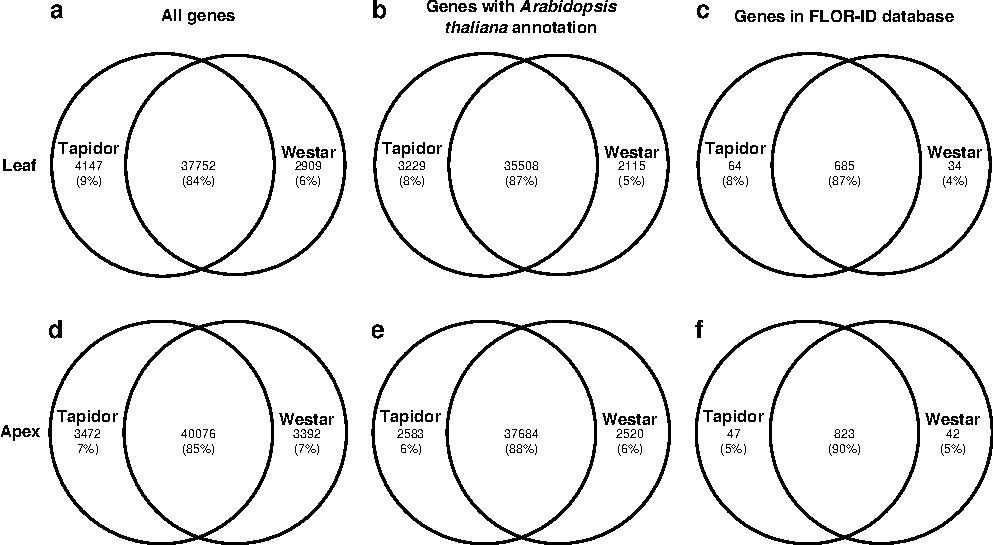
\includegraphics{figuredirectory/variety_venn_diagram.pdf}
\caption{\textbf{Overlap between varieties in the sets of expressed
genes.} \emph{B. napus} genes were regarded as expressed if their
maximal expression level across the transcriptomic time series was
greater than, or equal to, 2~FPKM. The overlaps in the leaf reveal a
greater number of variety specific expression in Tapidor, with
43~-~88~\% more genes than Westar. This is the case regardless of the
gene subset taken. This finding is not as evident in the apex. The gene
subsets used to calculate the overlaps in each case are: \textbf{a} and
\textbf{d} All \emph{B. napus} genes; \textbf{b} and \textbf{e} \emph{B.
napus} genes with identifiable Arabidopsis homologues; \textbf{c} and
\textbf{f} \emph{B. napus} genes that show sequence similarity to
Arabidopsis genes in the FLOR-ID database of floral genesTODOREF.
Percentages have been rounded to the closest
integer.}\label{figure:3xx:varietyvenn}
\end{figure}

As flowering in Tapidor is dependent on experiencing a period of cold,
the plant potentially has an increased ability to sense its environment
relative to a spring variety. This expansion in sensory ability could be
mediated through the expression of additional genes in the winter
variety relative to the spring variety. To investigate this, the overlap
between the expressed \emph{B. napus} genes in each variety was
calculated. In the leaf 4~\% to 6~\% of genes exhibit spring specific
expression, whereas 8~\% to 9~\% show winter specific expression (Figure
\ref{figure:3xx:varietyvenn}). The bias towards Tapidor increases when
floral genes are considered; there are 43~\% more Tapidor specific genes
than Westar when all \emph{B. napus} genes are considered (Figure
\ref{figure:3xx:varietyvenn}a), 53~\% when only \emph{B. napus}
homologues of Arabidopsis genes are considered (Figure
\ref{figure:3xx:varietyvenn}b), and 88~\% when \emph{B. napus} floral
genes are considered (Figure \ref{figure:3xx:varietyvenn}c). This bias
was not observed to the same extent in the apex, where all \emph{B.
napus} and \emph{B. napus} genes with identified Arabidopsis homologues
only showed 2~\% and 3~\% more Tapidor specific genes relative to
Westar, with 12~\% more among floral genes. There therefore seems to be
a consistent bias towards Tapdior having more variety specific genes
expressed in the leaf.

\begin{figure}[htbp]
\centering
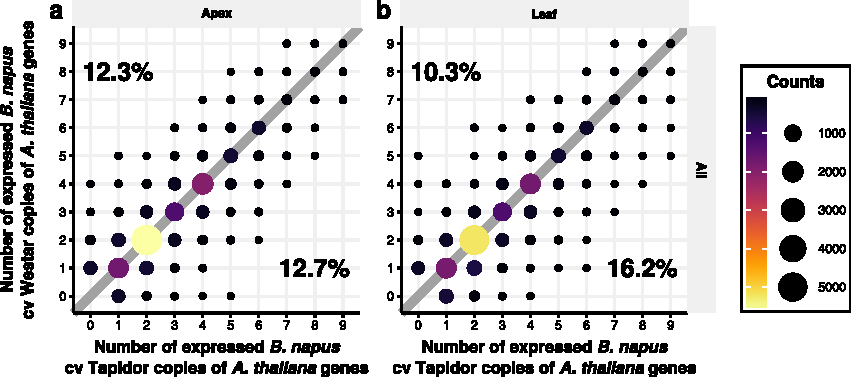
\includegraphics{figuredirectory/tap_vs_wes_exp_all.pdf}
\caption{\textbf{Relationship between the number of expressed copies of
Arabidopsis genes in Tapidor relative to Westar.} The number of
expressed copies of an Arabidopsis gene in \emph{B. napus} was
determined as the number of homologues that had a maximal expression
value above or equal to 2~FPKM at at least one time point in the time
series. The size and colour of the circles indicate the number of data
points at that position. Points on the diagonal, grey line represent
Arabidopsis genes that have equal numbers of homologues expressed in
both Tapidor and Westar. The left most percentage within each graph
represent the number of Arabidopsis genes that have more homologues
expressed in Westar, whereas the right most percentage is the
corresponding percentage for Tapidor. In both the apex (\textbf{a}) and
the leaf (\textbf{b}) there are more Arabidopsis genes with more copies
expressed in Tapidor relative to Westar, although this bias is
exaggerated in the leaf relative to the
apex.}\label{figure:3xx:tapvswesall}
\end{figure}

The bias towards Tapidor specific expression observed from the overlaps
of expressed genes (Figure \ref{figure:3xx:varietyvenn}) does not take
into account homologue relationships. For example, within a set of
\emph{B. napus} genes homologous to the same Arabidopsis gene, variety
specific expression of one homologue towards one variety and another
homologue towards the other variety would result in the same number of
homologues being expressed in each variety. This phenomenon will be
described as compensatory expression of homologues. In order to
investigate whether this form of compensation takes place, the number of
Tapidor expressed and the number of Westar expressed copies of each
Arabidopsis gene were compared (Figure \ref{figure:3xx:tapvswesall}). In
the apex, 12.3~\% of Arabidopsis genes have more copies expressed in
Westar relative to Tapdior, while 12.7~\% show the converse relationship
(Figure \ref{figure:3xx:tapvswesall}a). However, the percentages
calculated using expression data from the leaf (Figure
\ref{figure:3xx:tapvswesall}b) reveal a higher percentage of Arabidopsis
genes have a greater number of homologues expressed in Tapidor (16.2~\%)
relative to Westar (10.3~\%). Within the range of 0 to 9 expressed
\emph{B. napus} homologues, the maximal difference in the number of
expressed homologues between varieties is 5 (Figure
\ref{figure:3xx:tapvswesall}). Percentages of Arabidopsis genes
exhibiting different numbers of expressed homologues in each variety are
higher than the percentages of \emph{B. napus} genes exhibiting variety
specific expression (Figure \ref{figure:3xx:varietyvenn}). For example,
10.3~\% of Arabidopsis genes have more homologues expressed in the leaf
in Westar relative to Tapidor (Figure \ref{figure:3xx:tapvswesall}b),
whereas 5~\% of \emph{B. napus} genes are expressed specifically in
Westar (Figure \ref{figure:3xx:varietyvenn}b). Given that the mapping of
Arabidopsis genes to \emph{B. napus} is one-to-many, this suggests that
\emph{B. napus} genes exhibiting variety specific expression are
generally well distributed among different Arabidopsis genes.

\begin{figure}[htbp]
\centering
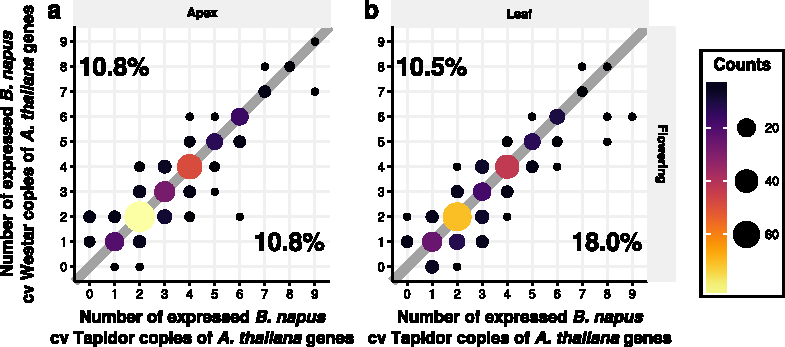
\includegraphics{figuredirectory/tap_vs_wes_exp_flowering.pdf}
\caption{\textbf{Relationship between the number of expressed copies of
Arabidopsis floral genes in Tapidor relative to Westar.} The number of
expressed copies of an Arabidopsis floral gene in \emph{B. napus} was
determined as the number of homologues that had a maximal expression
value above or equal to 2~FPKM at at least one time point in the time
series. The size and colour of the circles indicate the number of data
points at that position. Points on the diagonal, grey line represent
Arabidopsis floral genes that have equal numbers of homologues expressed
in both Tapidor and Westar. The left most percentage within each graph
represent the number of Arabidopsis genes that have more homologues
expressed in Westar, whereas the right most percentage is the
corresponding percentage for Tapidor. In both the apex (\textbf{a})
there are equal numbers of Arabidopsis floral genes on both sides of the
diagonal, whereas in the leaf (\textbf{b}) there are more Arabidopsis
genes with more copies expressed in Tapidor relative to
Westar.}\label{figure:3xx:tapvswesflor}
\end{figure}

To test if the retention of flowering time genes would affect the
observation of Arabidopsis genes tending to have more expressed
homologues in Tapidor leaf tissue, this was tested using a subset of
flowering time genes. In the apex (Figure
\ref{figure:3xx:tapvswesflor}a) a higher percentage of Arabidopsis genes
have the same number of homologues expressed in both varieties (78.4~\%)
relative to the global percentage (75.0~\%). This suggests that the
functions of multiple copies of flowering time genes may tend to be more
conserved between varieties that the rest of the genes in the genome,
although further validation would be required. An alternative
explanation is that compensatory expression of homologues occurs more
frequently among floral genes. The observed bias towards Arabidopsis
genes having more expressed genes in Tapidor is slightly exaggerated
when floral genes are considered separately (Figure
\ref{figure:3xx:tapvswesflor}b). These findings reveal that flowering
time genes exhibit less variety specific expressed homologue counts in
the apex, yet the bias towards Arabidopsis genes having more expressed
homologues in the winter variety is slightly exaggerated.

\begin{figure}[htbp]
\centering
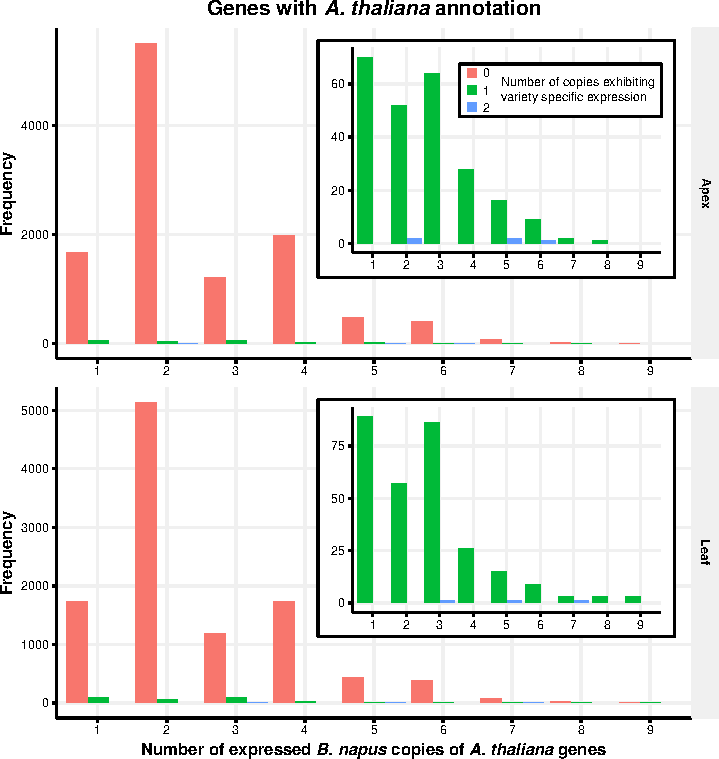
\includegraphics{figuredirectory/var_specific_distribution_all.pdf}
\caption{\textbf{Extent of compensatory homologue expression.} Only
Arabidopsis genes that have the same number of homologues expressed in
both Tapidor and Westar (points that lie on the diagonal grey line in
Figure \ref{figure:3xx:tapvswesall}) are considered. These are separated
by those that have 0, 1, or 2 homologues that exhibit compensatory
expression behaviour. The inset displays the same data as the main
figure, but without the bars corresponding to Arabidopsis genes with
zero homologues that exhibit compensatory behaviour. Very few instances
of compensation are observed between homologues in both the apex,
\textbf{a}, and the leaf, \textbf{b}.}\label{figure:3xx:varspecificall}
\end{figure}

The occurrence of compensatory expression between homologues could
represent a form of varietal differentiation. The extent of compensatory
expression was assessed among Arabidopsis genes that have the same
number of copies expressed in both \emph{B. napus} varieties (75.0~\%
for the apex, 73.5~\% for the leaf; diagonal grey lines in Figure
\ref{figure:3xx:tapvswesall}). For the vast majority of cases (98~\% in
the apex, 97~\% in the leaf) the same complement of gene copies were
expressed in both varieties (Figure \ref{figure:3xx:varspecificall}).
The maximal number of copies showing compensatory variety specific
expression is two, which represents instances where six copies of the
gene are expressed across both varieties, four in each. However, the
instances of this are low.

\begin{figure}[htbp]
\centering
\includegraphics{figuredirectory/var_specific_distribution_flowering.pdf}
\caption{\textbf{Extent of compensatory homologue expression among
floral genes.} Only Arabidopsis flowering time genes that have the same
number of homologues expressed in both Tapidor and Westar (points that
lie on the diagonal grey line in Figure \ref{figure:3xx:tapvswesflor})
are considered. These are separated by those that have 0 or 1 homologues
that exhibit compensatory expression behaviour. The inset displays the
same data as the main figure, but without the bars corresponding to
Arabidopsis flowering time genes with zero homologues that exhibit
compensatory behaviour. Very few instances of compensation are observed
between homologues in both the apex, \textbf{a}, and the leaf,
\textbf{b}.}\label{figure:3xx:varspecificflor}
\end{figure}

Similar patterns are observed with the floral genes, with 98~\% of genes
in both tissues having the same complement of gene copies expressed in
both varieties (Figure \ref{figure:3xx:varspecificflor}). These results
indicate that the occurrence of compensatory homologue expression is
comparatively rare, with floral genes having little effect on this
pattern.

Taken together these results illustrate that variety specific expression
of \emph{B. napus} genes occurs, although the majority of genes do not
exhibit it. There are more \emph{B. napus} genes expressed specifically
expressed in Tapidor in the leaf relative to the apex (Figure
\ref{figure:3xx:varietyvenn}), with the difference in the number of
variety specific genes increasing when a subset of floral genes are
taken. At the Arabidopsis gene level, approximately a quarter of
Arabidopsis genes exhibit differences in the number of \emph{B. napus}
homologues expressed in each variety (Figure
\ref{figure:3xx:tapvswesall}). Once again, the leaf specific bias
towards Tapidor specific expression is maintained (Figure
\ref{figure:3xx:tapvswesall}). This tissue dependent bias towards
Tapidor having a greater number of expressed homologues in the leaf
raises the possibility that the additional copies are required for
processes occurring in the leaf in Tapidor that are not occurring in
Westar. In addition, \emph{B. napus} homologues of the same Arabidopsis
gene compensating for each other between varieties is a relatively rare
occurrence (Figure \ref{figure:3xx:varspecificall}). This suggests that
this potential form of varietal divergence does not play a role in
phenotypic differences between the varieties, or if it does play a role,
that it is the effect of relatively few genes.

\subsection{Self-organizing maps reveal that a cold requirement delays
developmental transcriptional programs}\label{section:winter:som}

\begin{figure}[htbp]
\centering
\includegraphics{figuredirectory/tapidor_apex_som.pdf}
\caption{\textbf{Self-organizing map of the apex transcriptome in
Tapidor.} Gene expression patterns were normalized to zero mean, unit
variance across time and clustered. Nodes (coloured circles) are
situated adjacent to nodes with a similar expression pattern. The nodes
on the edges of the map are adjacent to the nodes on the opposing side
of the map, such that the map, when viewed in three dimensions, would
form a toroid. The colour of the circle indicates the number of genes
mapped to that particular node. The three clusters with the most genes
mapped to them are 46, exhibiting an increase in expression at the final
time point, and 88 and 98, with the expression pattern of both clusters
increasing during the vernalization
treatment.}\label{figure:3xx:tapsomapex}
\end{figure}

To understand whether a vernalization requirement has large scale
effects on gene expression, self-organizing maps (SOMs) were used to
cluster gene expression profiles across time. This was done to determine
if the vernalization response acts through relatively few genes that
have a large effect on flowering, or by affecting gene expression on a
global scale. SOMs were employed to allow broad comparisons in
regulatory patterns to be made between the two varieties. The SOM
clusters to which most genes mapped in Tapidor showed remarkable
similarity to the SOM clusters containing most genes in the spring
variety (section \ref{section:spring:experimentaldesign}). In the apex
(Figure \ref{figure:3xx:tapsomapex}) clusters 88 and 98 both exhibit
increased expression during the vernalization period, with expression
returning to pre-cold levels after the treatment. This expression trace
closely follows that of cluster 19 from the Westar apex SOM (Figure
\ref{figure:216:somaw}). Likewise, cluster 46 from both the Tapidor and
Westar apex SOMs (Figure \ref{figure:3xx:tapsomapex} and
\ref{figure:216:somaw}) exhibit relatively constant expression during
the entire time series, with expression increasing significantly between
the penultimate and final time points. However, although a similar
pattern is observed, the final time point in the Tapidor time series (83
days of growth) does not occur at the same time as the final time point
of the Westar time series (72 days of growth). Therefore, the
upregulation of genes in Tapidor cluster 46 is delayed relative to
Westar. The most highly enriched GO terms for this cluster relate to
carpel, gynoecium, and floral whorl development, which is consistent
with the vernalization response delaying flowering in the winter
variety. Clusters 88 and 98 are both enriched for the GO term
``circadian rhythm''. That the expression of these clusters is very
similar to clusters in Westar suggests that the vernalization
requirement does not influence the expression of genes associated with
the circadian rhythm or the photoperiod flowering pathway.

\begin{figure}[htbp]
\centering
\includegraphics{figuredirectory/tapidor_leaf_som.pdf}
\caption{\textbf{Self-organizing map of the leaf transcriptome in
Tapidor.} Gene expression patterns were normalized to zero mean, unit
variance across time and clustered. Nodes (coloured circles) are
situated adjacent to nodes with a similar expression pattern. The nodes
on the edges of the map are adjacent to the nodes on the opposing side
of the map, such that the map, when viewed in three dimensions, would
form a toroid. The colour of the circle indicates the number of genes
mapped to that particular node. The two clusters with the most genes
mapped to them are 59, exhibiting an increase in expression after the
vernalization treatment, and 25, the expression pattern of which
increases during the vernalization
treatment.}\label{figure:3xx:tapsomleaf}
\end{figure}

Similarities to Westar were also observed in the SOM generated using the
leaf transcriptomes from Tapidor, with two clusters having many genes
mapped to them (Figure \ref{figure:3xx:tapsomleaf}). Cluster 25 exhibits
in increase during the vernalization treatment (Figure
\ref{figure:3xx:tapsomleaf}), similarly to cluster 99 in the Westar leaf
SOM (Figure \ref{figure:217:somlw}). Both clusters are enriched for GO
terms linked to translation and protein biosynthesis, suggesting that
the response to cold in the leaf requires the synthesis of novel
cellular component. The other cluster with a large number of genes
mapped to it in the Tapidor leaf SOM is cluster 59, that exhibits a
slight increase in expression post-cold and a large increase at the
final time point (Figure \ref{figure:3xx:tapsomleaf}). This is a similar
expression trace to that exhibited by cluster 19 in the Westar leaf SOM
(Figure \ref{figure:217:somlw}). The GO terms enriched in these two
clusters relate to responding to cell stress, ageing and cell death. As
with the apex, therefore, it seems that a requirement for cold delays
the expression of genes that are expressed later in development but does
not affect genes expressed as a result of the cold-treatment.

In order to compare transcriptional responses between tissues,
comparisons between the apex and leaf SOMs were made. By comparing
expression differences between the tissues in both varieties, it allows
for differences that are biologically relevant, and not the result of
biological noise, to be highlighted. Of the clusters to which most genes
are mapped in all SOMs generated, there is consistently a cluster with
an expression pattern that increases during the vernalization treatment,
with expression returning to pre-cold levels after the treatment. Tissue
specific subtleties exist between the expression traces for these
clusters. In the apex, the peak expression value during the cold is
observed at the day 43 time point in both Westar (cluster 19; Figure
\ref{figure:216:somaw}) and Tapidor (cluster 88; Figure
\ref{figure:3xx:tapsomapex}), with expression decreasing slightly at the
day 64 time point before returning to pre-cold levels after the
treatment. However, the response in the leaf is more gradual, with
expression increasing during the cold treatment and peaking at the day
64 time point in both Westar (cluster 99; Figure \ref{figure:217:somlw})
and Tapidor (cluster 25; Figure \ref{figure:3xx:tapsomleaf}). A
potential explanation is the difference in mitotic activity between the
two tissues\textsuperscript{371}. A mitotically active tissue, such as
the apex, potentially responds to environmental stimuli more quickly
than tissues where cell division is not as prolific, such as the leaf.
The mitotic activity of a tissue has been proposed to influence the
ability of that tissue to become vernalized\textsuperscript{367,368}.
The slower response to the cold treatment in the leaf may therefore be
due to the lack of cell division inhibiting the rate at which
vernalization directed transcriptional changes occur. The GO terms also
suggest differences in the genes mapped to these clusters, with the apex
clusters enriched for circadian rhythm genes and the leaf clusters
enriched for genes associated with translation. It may, therefore, be
that these clusters actually represent different ensembles of genes,
with the transcriptional program in the apex responding to photoperiod
changes and expression in the leaf responding to a requirement for novel
cellular components.

\subsection{Correlation analysis suggests apex and leaf transcriptomes
behave differently during plant
development}\label{section:winter:correlation}

The SOM analysis revealed that a vernalization requirement delays the
upregulation of genes associated with flower development in the apex,
which is expected. However, it also seems to delay the upregulation of
stress, cell death, and age related genes in the leaf, suggesting that a
vernalization requirement delays development more generally than just
delaying the floral transition. To investigate how the timing of
transcriptomic changes compare between the two varieties, Pearson
correlation coefficients were calculated between time points. Pearson
correlation coefficients are calculated by determining how linear the
relationship is between the FPKM values from one sample and the FPKM
values from another sample. A coefficient of 1 indicates a positive,
linear relationship between the gene FPKM values between samples,
whereas a coefficient of 0 indicates that a linear relationship is not
present. The coefficients were calculated both within and across
varieties for each tissue; the within variety comparisons allow for the
timing of transcriptional changes to be determined while the across
variety comparisons allow for differences in these timings, if they
exist, to be assessed.

\begin{figure}[htbp]
\centering
\includegraphics{figuredirectory/apex_correlation.pdf}
\caption{\textbf{Pearson correlation coefficients between apex samples.}
Coefficients were calculated between the transcriptomes of all apex
samples, with Westar-Westar (\textbf{a}), Westar-Tapidor (\textbf{b}),
and Tapidor-Tapidor (\textbf{c}) comparisons scaled individually.
Coefficients between like samples (diagonal lines in \textbf{a} and
\textbf{c}) have been removed for clarity. The higher the coefficient
value, the more similar two samples are. It should be noted that
although there are seven time points for Westar and Tapidor, the final
two time points in Westar (69 and 72 days) are different to the final
two time points in Tapidor (72 and 83 days)}\label{figure:3xx:corrapex}
\end{figure}

The first observation that stands out is the baseline similarity in
expression values between samples. The lowest correlation coefficient
observed is 0.4, which is found between the day 43 and day 83 samples
within the Tapidor leaf (Figure \ref{figure:3xx:corrleaf}). That there
is this basal level of correlation between the samples suggests that
many genes are regulated similarly in both varieties. Calculating
correlation values between tissues results in coefficients that are much
lower, with means of 0.35 (Westar) and 0.31 (Tapidor), suggesting that
the basal level of correlation observed between varieties is a
consequence of tissue specific gene expression.

\begin{figure}[htbp]
\centering
\includegraphics{figuredirectory/leaf_correlation.pdf}
\caption{\textbf{Pearson correlation coefficients between leafsamples.}
Coefficients were calculated between the transcriptomes of all leaf
samples, with Westar-Westar (\textbf{a}), Westar-Tapidor (\textbf{b}),
and Tapidor-Tapidor (\textbf{c}) comparisons scaled individually.
Coefficients between like samples (diagonal lines in \textbf{a} and
\textbf{c}) have been removed for clarity. The higher the coefficient
value, the more similar two samples are. The additional time point in
Tapidor results in the rectangular Westar-Tapidor comparison
heatmap.}\label{figure:3xx:corrleaf}
\end{figure}

An expectation of a correlation analysis such as this is that time
points within a variety would tend to be most similar to temporally
proximal time points, with similarity decreasing as time passes. This is
based on the assumption that global transcriptional changes take time to
orchestrate. Such behaviour is observed between samples from the same
variety, with the patterns being observed most clearly post-cold, from
the day 65 time point onwards (Figures \ref{figure:3xx:corrapex} and
\ref{figure:3xx:corrleaf}). For example, in both tissues from Tapidor
the day 22 time point is most highly correlated with the day 65 time
point, with the size of the coefficient decreasing as time progresses.
In addition, adjacent time points post-cold are generally highly
correlated (Figures \ref{figure:3xx:corrapex} and
\ref{figure:3xx:corrleaf}), suggesting that the transcriptional time
series captures dynamic changes in expression. This pattern is not as
clear in Westar however, with all three time points sampled immediately
after cold in the apex (day 65, 67, and 69; Figure
\ref{figure:3xx:corrapex}a) and the two post-cold time points in the
leaf (day 65 and day 67; Figure \ref{figure:3xx:corrleaf}a) being highly
correlated. This indicates that large scale changes in transcription
were only observed between the day 69 and day 72 time points in both
tissues in the Westar samples. This is in contrast to Tapidor, where
transcriptional changes occurred more slowly post-cold (Figures
\ref{figure:3xx:corrapex}c and \ref{figure:3xx:corrleaf}c). The cold
treatment results in a transcriptional landscape distinct from the other
time points. In both varieties, and in both tissues, the day 43 time
point (half way through the vernalization treatment) has the highest
correlation with the other time point taken during cold; the day 64 time
point sampled the day before plants were removed from cold. This is also
exemplified by the day 22 time point having the highest correlation with
the day 65 time point in both varieties and tissues; the first time
point sampled after the plants were removed from the cold treatment.
This reveals both that the cold treatment has a large effect on the
transcriptome, and that the transcriptome, at a global level, responds
quickly to removal from cold by returning to a largely similar state as
pre-cold.

The most striking result from this analysis is in the comparisons
between varieties for both tissues (Figures \ref{figure:3xx:corrapex}b
and \ref{figure:3xx:corrleaf}b). In the leaf, the highest correlation
coefficients are between samples taken at the same time point (Figure
\ref{figure:3xx:corrleaf}b). The exception to this is the day 83 time
point from Tapidor, as there is no corresponding sample taken for
Westar. This trend, however, does not apply to the entire time series in
the apex samples. The highest correlation coefficients for the Tapidor
samples at day 22, day 43, and day 64 are the Westar samples from the
corresponding time points (Figure \ref{figure:3xx:corrapex}b). The day
65 time point in Tapidor is most correlated with the day 22 time point
in Westar, although the day 65 time point has the second highest
coefficient. This is likely due to the confounding effects of day 22 and
day 65 time points being highly correlated within variety. After the day
65 time point, however, the most highly correlated sample does not
correspond to the samples taken on the same day. The day 67 and day 72
samples from Tapidor are most highly correlated with the day 67 time
point in Westar. The two final time points are also most highly
correlated, despite the Tapidor sample being sampled 83 days post-sowing
and the Westar sample 72 days post-sowing (Figure
\ref{figure:3xx:corrapex}b). Taken together these two results suggest
that different factors are having influencing the transcriptome in each
tissue. The equivalent time points being most highly correlated in the
leaf suggests that the age of the leaf is having the largest effect on
the transcriptome. That there is a time delay between the most highly
correlated samples in the apex suggests that age does not influence the
transcriptome in the apex as strongly as the leaf. Instead, the pattern
of correlation coefficients suggests that developmental stage influences
the transcriptome in the apex. This is seen most clearly at the final
time point, which was sampled such that the two varieties were at a
similar developmental stage (BBCH stage 51\textsuperscript{239}).

\subsection{Conclusions}\label{conclusions-4}

To investigate whether a cold requirement impacts the \emph{B. napus}
transcriptome at the global level, or as a more focussed effect, the
transcriptomes from both Tapidor and Westar across the time series were
compared. Analysis of variety specific expression of \emph{B. napus}
genes, and of variety specific numbers of expressed homologues for
Arabidopsis genes , reveals that there are more Tapidor specific
\emph{B. napus} genes than Westar in the leaf. The leaf is the plant
organ at which photoperiod is interpreted\textsuperscript{17,18,20--22}
and also plays a role in sensing the vernalization
response\textsuperscript{28,227,366}. An expanded set of genes expressed
exclusively in Tapidor could represent increased sensory machinery in
the leaf in the winter variety relative to the spring variety, in line
with the increased vernalization sensitivity of Tapidor. This is
especially interesting given that \emph{FLC} has been found to influence
the activity of the circadian clock\textsuperscript{377} In addition, it
is interesting that the percentage of \emph{B. napus} genes expressed in
both varieties (Figure \ref{figure:3xx:varietyvenn}) is larger than the
percentage of genes expressed in both tissues in Westar (Figure
\ref{figure:211:venn}). This reveals that the occurrence of variety
specific expression is lower than tissue specific expression within a
variety, suggesting that the tissue dissection was successful at
enriching for apex tissue.

The results from the SOM clustering reveals that, in the apex, the
vernalization requirement delays the upregulation of genes enriched for
GO terms associated with flower development. This is fully expected
given the role the vernalization pathway plays in repressing the floral
transition. What the correlation analysis uncovers, however, is that
global transcriptional responses are also delayed in Tapidor relative to
Westar. Therefore, in the apex, vernalization seems to have a large
effect on the transcriptome to delay development. This suggests the
developmental stage of the plant has a large effect on the transcriptome
in the apex. Vernalization also seems to delay the upregulation of genes
associated with stress responses, cell death, and aging at the final
time point in the Tapidor leaf samples, relative to the Westar leaf
samples. However, the correlation analysis suggests that the
transcriptome of the leaf is affected more by the age of the tissue,
rather than the developmental stage of the plant as a whole like the
apex. This is likely a result of the first true leaf being sampled
throughout the experiment (discussed in section
\ref{section:spring:experimentaldesign}). The observed delay in the
upregulation of genes at the final time point in Tapidor is therefore
likely to be an artefact of the expression profile normalization
procedure.

\section{\texorpdfstring{\emph{B. napus} vernalization pathway
regulatory
divergence}{B. napus vernalization pathway regulatory divergence}}\label{section:winter:vern}

The vernalization response is arguably one of the most investigated
floral pathways in \emph{Brassica}
crops\textsuperscript{116,133,134,137,140,143}, likely due to its
agronomic importance\textsuperscript{116,123}. Work has also been
motivated by \emph{FLC} and \emph{FRI} homologues in \emph{Brassica}
crops being found in regions of the genome statistically associated with
flowering time variation\textsuperscript{128--139}. Molecular
characterisation has also identified the importance of vernalization
pathway genes, with between variety polymorphisms at the \emph{FLC}
locus responsible for heading data variation in \emph{B.
oleracea}\textsuperscript{136}. However, aside from the association
studies, the interactions between the copies of vernalization genes
\emph{in planta} have not been assessed. Even within the association
studies, although large phenotypic effects were attributed to certain
vernalization gene homologues, more subtle variation attributable to
other homologues might be masked. The importance of considering the
effects of multiple homologues on the floral transition is perfectly
exemplified with \emph{FLC}. Not only have the dosage effects of the
gene been revealed\textsuperscript{371}, but the long non-coding RNA
expressed from the \emph{FLC} locus also has the potential of acting in
trans to influence the expression of other \emph{FLC} loci in the
genome\textsuperscript{349,378}.

To investigate whether \emph{B. napus} homologues of Arabidopsis
vernalization pathway genes are mediating the difference in
vernalization requirement between Tapidor and Westar, the behaviour of
the genes was assessed in the transcriptomic time series. From analysing
the expression of \emph{FLC}, \emph{FRI}, and PRC2 component genes, in
both Westar and Tapidor, \emph{BrFLC} genes emerge as being the most
likely candidates for mediating the difference in flowering time between
Tapidor and Westar. Specifically, \emph{BrFLC} genes on A10, A2 and A3
show variety specific responses, suggesting these copies are responsible
for the requirement for cold that Tapidor plants require in order to
flower. \emph{BrFLC} genes on chromosomes C2 and A3 exhibit cold induced
silencing of expression in both varieties, suggesting that these copies
are responsible for the vernalization response observed in
Westar\textsuperscript{234}. No apparent tissue specificity was present
between the \emph{BrFLC} genes, suggesting that spatial
subfunctionalization\textsuperscript{202,209} has not taken place.

\subsection{\texorpdfstring{\emph{FLOWERING LOCUS
C}}{FLOWERING LOCUS C}}\label{section:winter:flc}

\begin{figure}[htbp]
\centering
\includegraphics{figuredirectory/apex_tapidor_flc.pdf}
\caption{\textbf{Expression traces for the \emph{BnFLC} genes in the
apex of Tapidor.} The expression values and the 95\% confidence
intervals of those expression values as computed by Cufflinks are
displayed. A heatmap of the clustering coefficients calculated by the
SOM based method (discussed in section
\ref{section:spring:somexplanation}) quantifies the similarity between
the expression profiles. The A2, A10, A3 and C3 copies show very similar
expression traces. The C2 copy behaves similarly to the A3b and C3
copies. The C9 copies are similar to each other, but have expression
profiles that are different from the other \emph{BnFLC}
copies.}\label{figure:3xx:flctapapex}
\end{figure}

\begin{figure}[htbp]
\centering
\includegraphics{figuredirectory/apex_westar_flc.pdf}
\caption{\textbf{Expression traces for the \emph{BnFLC} genes in the
apex of Westar.} The expression values and the 95\% confidence intervals
of those expression values as computed by Cufflinks are displayed. A
heatmap of the clustering coefficients calculated by the SOM based
method (discussed in section \ref{section:spring:somexplanation})
quantifies the similarity between the expression profiles. All copies,
except the C9b copy, show similar expression
traces.}\label{figure:3xx:flcwesapex}
\end{figure}

The product of the \emph{FLC} gene in Arabidopsis is the central
regulator of the vernalization pathway\textsuperscript{26,371}. Given
that \emph{FLC} copy number in Arabidopsis impacts floral growth in a
dosage dependent manner\textsuperscript{371} and that the gene product
seems to have contrasting roles in both the leaf and
apex\textsuperscript{227}, a key question is whether the copies in
\emph{B. napus} exhibit regulatory divergence. In order to assess
whether this is the case, it is important to consider the expression of
the gene in both the apex and the leaf, as it has been found that
\emph{FLC} plays roles in both\textsuperscript{227}. In the
developmental time series, across both tissues and varieties, ten copies
of \emph{BnFLC} are expressed above 2.0 FPKM at at least one time point;
four on the A genome and six on the C genome. The complement of copies
expressed, however, varies based on the tissue and variety investigated.

In the Tapidor apex, nine copies of \emph{BrFLC} are expressed, and
exhibit a \emph{mixed} pattern of regulatory module assignment,
indicating regulatory divergence (Figure \ref{figure:3xx:flctapapex}).
The largest of these regulatory modules consist of all A genome
\emph{BnFLC} genes and the two \emph{BnFLC.C3}. These genes are grouped
together as all exhibit a decrease in expression during the
vernalization period, with expression remaining low post cold. This
pattern of expression mirrors that of \emph{FLC} from
Arabidopsis\textsuperscript{28}. \emph{BnFLC.C2} also decreases during
the vernalization period, but the repression is not stable, and
reactivation is observed post-cold (Figure \ref{figure:3xx:flctapapex}).
This pattern of \emph{FLC} expression has been observed in Arabidopsis
lines that have not been given sufficient cold exposure to result in the
stable repression of \emph{FLC}\textsuperscript{238,343}. A partial
reactivation of \emph{BnFLC.A3b}, \emph{BnFLC.C3b}, and \emph{BnFLC.C3c}
results in the clustering coefficient of these copies and the
\emph{BnFLC.C2} copy being high. Finally, the \emph{BnFLC.C9a} and
\emph{BnFLC.C9b} have similar expression traces in the time series, with
both genes having relatively low expression before and during cold, with
an increase in expression post-cold. Interestingly the \emph{BnFLC.C9b}
gene seems to increase during cold, an expression behaviour that to the
best of my knowledge has not been observed for \emph{FLC} in
Arabidopsis.

Seven of the nine \emph{BnFLC} copies expressed in Tapidor apex are also
expressed in Westar apex, with the \emph{BnFLC.A10} and \emph{BnFLC.C3c}
copies being the two lacking expression in the spring variety relative
to the winter variety (Figure \ref{figure:3xx:flcwesapex}). Given that
the A10 copy was relatively highly expressed in the winter variety, this
supports findings that this copy is the main copy driving the
requirement for cold in \emph{B. napus}\textsuperscript{130,137--139}.
All copies except the \emph{BnFLC.C9b} copy decrease in expression
during the vernalization period, with expression remaining low after the
treatment, resulting in high clustering coefficients between these
copies. The \emph{BnFLC.C3b} copy shows slight reactivation after the
cold treatment, leading to it having lower clustering coefficients
relative to the other genes in the regulatory module (Figure
\ref{figure:3xx:flcwesapex}). As was the case in Tapidor,
\emph{BnFLC.C9b} shows a markedly different expression trace, exhibiting
a slight increase in expression halfway through vernalization, with an
increase in expression post-cold.

Analysis of the expression traces in the apex in both Tapidor and Westar
reveals that all \emph{BnFLC} genes, except \emph{BnFLC.C9b}, decrease
in expression during the cold treatment. The A10 and C3c copy are
expressed in the winter variety, yet lack expression in the spring
variety. Some copies exhibit reactivation after the cold-induced
decrease, suggesting that the vernalization treatment was not sufficient
to stably silence those copies. Interestingly, this reactivation seems
to be variety specific for some genes, with the A3b, C2, and C9a copies
exhibiting reactivation in the winter and not the spring variety.

\begin{figure}[htbp]
\centering
\includegraphics{figuredirectory/flc_comparison_apex_1.pdf}
\caption{\textbf{Expression traces for the A genome \emph{BnFLC} genes
commonly expressed in the apex of both varieties.} The expression values
and the 95\% confidence intervals of those expression values as computed
by Cufflinks are displayed. The A2 and A3b copies exhibit varietal
differences in the magnitude of expression at the pre-cold time point,
in line with these copies delaying the floral transition in Tapidor
relative to Westar. The A3a copy is similarly expressed in both
varieties, suggesting it does not contribute to the observed
delay.}\label{figure:3xx:flcapexagenome}
\end{figure}

\begin{figure}[htbp]
\centering
\includegraphics{figuredirectory/flc_comparison_apex_2.pdf}
\caption{\textbf{Expression traces for the C genome \emph{BnFLC} genes
commonly expressed in the apex of both varieties.} The expression values
and the 95\% confidence intervals of those expression values as computed
by Cufflinks are displayed. Variety specific differences in the
magnitude of expression at the pre-cold time point are consistent with a
role in the vernalization response. In contrast, the expression of the
C9b copies is frequently higher across the time series in the spring
variety, suggesting that these copies do not delay the floral
transition.}\label{figure:3xx:flcapexcgenome}
\end{figure}

The expression response of \emph{FLC} in Arabidopsis is quantitative, at
least at the tissue level at which we are
sampling\textsuperscript{28,359}. The magnitude of expression is
therefore an important aspect of \emph{FLC} regulation. Comparing the
expression traces of the A genome copies of \emph{BnFLC} expressed in
both varieties in the apex (Figure \ref{figure:3xx:flcapexagenome})
revealed that the A2 and A3b copies are initially expressed at
significantly lower levels in the spring variety relative to the winter
variety. Therefore, although these copies both exhibit a decrease in
expression during the cold treatment in both varieties, the absolute
difference in expression level is greatest in the winter variety. The
A3a copy of \emph{BnFLC} shows remarkably similar expression traces and
expression levels throughout the developmental time series in both
varieties. Differences in the magnitude of expression are also observed
for the C genome copies of \emph{BnFLC} (Figure
\ref{figure:3xx:flcapexcgenome}). Like the A2 and A3b copies,
\emph{BnFLC.C2} is more highly expressed pre-cold in the winter variety
relative to the spring variety, suggesting a role in delaying the floral
transition in Tapidor. The C3b copy of \emph{BnFLC} shows very similar
expression patterns and levels across the entire time series in both
varieties, and very lowly expressed in general. This suggests that it
does not contribute to the differences in flowering observed between the
two varieties. Finally, the C9 copies of \emph{BnFLC} are frequently
more highly expressed in the spring variety relative to the winter
variety. This is especially true for \emph{BnFLC.C9b}, where the
expression level of the gene in the spring variety is approximately 3
fold higher than the winter variety at the beginning of the time series.
That these copies are more highly expressed in the spring variety
indicates that these copies likely do not play a role in delaying the
floral transition, unlike the role of \emph{FLC} in Arabidopsis.

The expression of \emph{BnFLC} genes in the apex reveals that all but
one homologue decrease in expression during the cold treatment, in line
with expectations from Arabidopsis\textsuperscript{28}. That some copies
exhibit reactivation in the winter, and not the spring variety, suggests
that potentially the length of cold was not sufficient to stably repress
the expression of those copies. Comparing the magnitude of expression
between the copies reveals that the A2, A3b, A10, and C2 copies seem to
be more highly expressed in Tapidor at the beginning of the time series
relative to Westar. That these copies exhibit stable decreases in
expression during cold treatment and are highly expressed in Tapidor
makes them good candidates for being responsible for the delay in
flowering in the winter variety. The A3a copy, however, exhibits cold
induced stable repression in both varieties, indicating that it is
potentially responsible for the vernalization requirement of
Westar\textsuperscript{234}. Finally, the C9b copy is more highly
expressed in the spring variety relative to the winter variety and is
not repressed during the cold treatment. This indicates that this
particular copy of \emph{BnFLC} has diverged significantly in its
regulation relative to Arabidopsis \emph{FLC}, and is likely not
involved with mediating the vernalization response in \emph{B. napus}.

\begin{figure}[htbp]
\centering
\includegraphics{figuredirectory/leaf_tapidor_flc.pdf}
\caption{\textbf{Expression traces for the \emph{BnFLC} genes in the
leaf of Tapidor.} The expression values and the 95\% confidence
intervals of those expression values as computed by Cufflinks are
displayed. A heatmap of the clustering coefficients calculated by the
SOM based method (discussed in section
\ref{section:spring:somexplanation}) quantifies the similarity between
the expression profiles. All copies, except C9b, have similar expression
profiles as determined by the clustering
coefficients.}\label{figure:3xx:flctapleaf}
\end{figure}

\begin{figure}[htbp]
\centering
\includegraphics{figuredirectory/leaf_westar_flc.pdf}
\caption{\textbf{Expression traces for the \emph{BnFLC} genes in the
leaf of Westar.} The expression values and the 95\% confidence intervals
of those expression values as computed by Cufflinks are displayed. A
heatmap of the clustering coefficients calculated by the SOM based
method (discussed in section \ref{section:spring:somexplanation})
quantifies the similarity between the expression profiles. A
\emph{mixed} pattern of clustering coefficients is observed, with C9
copies being in separate regulatory modules and A2, C2, and A3a
exhibiting a gradiant of similarity.}\label{figure:3xx:flcwesleaf}
\end{figure}

To assess whether the \emph{BnFLC} genes exhibited tissue specific
expression, the expression of the genes was analysed in the leaf tissue.
In the Tapidor leaf samples eight copies of \emph{BnFLC} are detected as
expressed; all four copies from the A genome, \emph{BnFLC.C2},
\emph{BnFLC.C3a}, \emph{BnFLC.C3c}, and \emph{BnFLC.C9b} (Figure
\ref{figure:3xx:flctapleaf}). The \emph{BnFLC.C3a} copy is expressed in
the leaf and not the apex, whereas two \emph{BnFLC} genes
(\emph{BnFLC.C9a} and \emph{BnFLC.C3b}) are expressed in the apex and
not in the leaf. However, the expression of these genes in their
respective tissues is close to the 2.0 FPKM threshold used to determine
if genes are expressed or not, suggesting that the presence or absence
of these genes in the set of expressed genes is more heavily influenced
by noise relative to the other copies. This suggests that \emph{FLC}
homologues in \emph{B. napus} have not diverged in terms of spatial
expression domains. The genes expressed in the leaf have a
\emph{distinct} regulatory module assignment, with all the genes except
\emph{BnFLC.C9b} being assigned to the same regulatory module. The seven
genes assigned to the largest regulatory module all exhibit a decrease
in expression during the vernalization period to very low levels. In the
case of the A3a and C3a copies, this repression is very stable, whereas
the other genes show a slight reactivation of expression that peaks at
the day 72 time point before decreasing at the final time point. The
\emph{BnFLC.C9b} copy also decreases in expression during the
vernalization period, although the repression is not stable, with the
expression level increasing post-cold. This reveals that in the Tapidor
leaf, all expressed copies of \emph{BnFLC} exhibit a cold-induced
repression in expression, which in the case of \emph{BnFLC.C9b} is not
stable.

Fewer \emph{BnFLC} copies are expressed in the leaf in Westar relative
to Tapidor. The A10, A3b, and C3 copies are not expressed in the spring
variety, whereas the C9a copy is expressed in Westar and not Tapidor
(Figure \ref{figure:3xx:flcwesleaf}). That A10 and C3c show variety
specific expression in both the apex and leaf indicates that these
copies may delay the floral transition in the winter variety. In the
Westar leaf, \emph{mixed} pattern of regulatory module assignment is
observed, with four modules identified (Figure
\ref{figure:3xx:flcwesleaf}). The \emph{BnFLC.A2} and \emph{BnFLC.C2}
copies form one module, with both exhibiting decreases during the cold,
with partial reactivation post-cold. \emph{BnFLC.A2} is in another
regulatory module with \emph{BnFLC.A3a}, with the latter rapidly
decreasing in expression in response to cold and staying repressed after
the cold treatment. This intransitivity is likely due to the combination
of two differences between the \emph{BnFLC.A3a} and \emph{BnFLC.C2}
expression traces. The rate of decrease during the cold is more rapid in
the \emph{BnFLC.A3a} copy relative to the \emph{BnFLC.C2} copy, with the
former having a near zero expression level at the day 43 time point,
taken halfway through the cold treatment. The other behaviour that
differs is the post-cold treatment, with the \emph{BnFLC.C2} copy
showing partial reactivation unlike the \emph{BnFLC.A3a} copy. Different
rates of \emph{FLC} silencing and different reactivation dynamics are
also observed as natural variation in Arabidopsis\textsuperscript{238},
suggesting that the variation observed in the leaf tissue in Westar
between the A2, A3a, and C2 copies of \emph{BnFLC} may have biological
consequences. The two \emph{BnFLC} copies on the C9 chromosome are
located in regulatory modules that are unique to them. The
\emph{BnFLC.C9a} copy shows a partial increase in expression halfway
through the vernalization treatment, but returns to pre-cold expression
levels towards the end of cold and after the treatment. Although the
\emph{BnFLC.C9a} copy is expressed in the leaf in Westar and not
Tapidor, the expression of the gene only marginally exceeds the 2.0 FPKM
at a single time point, suggesting that its effect on flowering, if any,
will be minimal. Like the A2, C2, and A3a copies of \emph{BnFLC},
\emph{BnFLC.C9b} shows a decrease during the cold treatment, but also
displays a reactivation after the cold treatment.

The expression traces of \emph{BnFLC} genes in the leaf, like those from
the apex, reveal that the majority of copies respond to cold treatment
by decreasing in expression. Interestingly, the prevalence of
\emph{BnFLC} copies exhibiting reactivation in the leaf is less than in
the apex, potentially indicating that the apex in \emph{B.~napus} is
perennial in nature. The only copy that exhibits a significant change in
expression pattern between tissues is \emph{BnFLC.C9b}. In the apex this
copy does not exhibit cold-induced silencing, whereas it does in the
leaf. This suggests the C9b copy of \emph{BnFLC} exhibits
tissue-specific regulation in both varieties.

\begin{figure}[htbp]
\centering
\includegraphics{figuredirectory/flc_comparison_leaf.pdf}
\caption{\textbf{Expression traces for the \emph{BnFLC} genes commonly
expressed in the leaf of both varieties.} The expression values and the
95\% confidence intervals of those expression values as computed by
Cufflinks are displayed. Variety specific differences in the magnitude
of expression at the pre-cold time point for \emph{BnFLC.A2} and
\emph{BnFLC.C2} are consistent with a role in the vernalization
response. The response of the A3a copy to cold treatment is similar in
both varieties. In contrast, the expression of the C9b copy is more
highly expressed across the time series in the spring variety,
suggesting that this copy is not involved with delaying the floral
transition.}\label{figure:3xx:flcleafcgenome}
\end{figure}

Comparing between varieties (Figure \ref{figure:3xx:flcleafcgenome}),
similar differences in the magnitude of \emph{BnFLC} gene expression
were observed in the leaf as they were for the apex. Although
\emph{BnFLC.A2} demonstrates a similar response to cold in both Tapidor
and Westar, expression is approximately four fold higher in Tapidor
across the entire time series. Likewise, the C2 copy is expressed two
fold higher in Tapidor at the first time point relative to Westar, and
remains more highly expressed across the entire time series (Figure
\ref{figure:3xx:flcapexcgenome}). The differences in the magnitude of
expression in the leaf between the two varieties for the A2, A3b, A10,
and C2 copy of \emph{BnFLC} are consistent with the genes delaying the
floral transition in the winter variety. \emph{BnFLC.A3a} shows similar
expression levels in both the winter and spring variety in the leaf,
suggesting that this copy is not responsible for the delayed floral
transition in Tapidor. Finally, the \emph{BnFLC.C9b} copy is more highly
expressed in Westar throughout the entire time series, suggesting that
is does not play a role in the vernalization response in \emph{B.
napus}.

Taken together, this evidence indicates that the majority of
\emph{BnFLC} genes have retained a regulatory response to cold, and do
not exhibit significant tissue specificity in their expression. In the
apex in both varieties, all but one \emph{BnFLC} gene decreases in
expression during the cold. The same is also true in the leaf, although
the \emph{BnFLC} gene that does not exhibit a cold-induced decrease is
very lowly expressed and unlikely to have a significant role in the
plant. Within the apex in Tapidor, certain copies exhibit regulatory
divergence by reactivating in expression after cold. This behaviour
mirrors that of Arabidopsis accessions that have not received enough
cold to fully repress \emph{FLC}\textsuperscript{238,343} and \emph{FLC}
homologues in perennial relatives of
Arabidopsis\textsuperscript{163,379}. This suggests that these
particular copies of \emph{BnFLC} have not received sufficient cold to
be fully repressed, or the apex in Tapidor is somewhat perennial in
nature. The copy that exhibits most regulatory divergence is
\emph{BnFLC.C9b}. In the apex this copy increases in expression during
and after vernalization, while in the leaf cold-induced silencing is
observed but is not stable. This suggests that this particular copy does
not influence the vernalization response in \emph{B. napus}, and has
therefore acquired a separate function in the plant.

Comparing the magnitude of expression between varieties reveals copies
of \emph{BnFLC} that are likely to be mediating the delay in flowering
in Tapidor relative to Westar. The A2, A3b, A10, C2, and C3c copies of
\emph{BnFLC} are all expressed more highly in the winter variety than in
the spring. That all of these copies also exhibit cold induced silencing
makes them good candidates for mediating the delay in flowering in the
winter variety. Of particular interest are A2 and A10, as the silencing
of these copies is more stable post-cold than the others. This suggests
that one or both of these copies controls the vernalization requirement
of Tapidor, which the other copies, A3b, C2, and C3c, may mediate the
vernalization response. Comparing the magnitude of expression between
varieties also confirms the finding that \emph{BnFLC.C9b} is not
involved with delaying flowering time, as the gene is more highly
expressed in Westar relative to Tapidor.

Comparing expression data between the apex and the leaf reveals some
tissue specific expression. More copies of \emph{BnFLC} exhibit
reactivation in the Tapidor apex (Figure \ref{figure:3xx:flctapapex})
relative to the Tapidor leaf (Figure \ref{figure:3xx:flctapleaf}). This
supports the hypothesis that the Tapidor apex may have perennial
characteristics. In \emph{Arabidopsis halleri}, a perennial relative of
Arabidopsis, the expression of a \emph{FLC} homologue was found to
reactivate in young leaves\textsuperscript{379}. It is therefore likely
that \emph{BnFLC} reactivation is not observed in the leaf as the first
true leaf was sampled throughout the time series, such that the age
related effects and leaf senescence result in the lack of expression.
\emph{BnFLC.C9b} undergoes cold-induced silencing in the leaves of both
varieties, but does not do so in the apex. In addition, in Tapidor
samples, \emph{BnFLC.A3b} is expressed at approximately the same level
as \emph{BnFLC.A2} in the apex, whereas in the leaf the A3b copy is
expressed \textasciitilde{}2.5 fold lower than the A2 copy. These
findings suggests that some copies of \emph{BnFLC} are expressed in a
tissue specific manner. In the case of \emph{BnFLC.A3b}, potentially its
effect on a vernalization response is mediated predominantly in the
apex. This is interesting given the different roles \emph{FLC} has in
the apex and leaf in Arabidopsis\textsuperscript{227}.

\subsection{Polycomb repressive complex 2
proteins}\label{section:winter:prc2}

Most \emph{BnFLC} genes become silenced during cold in a similar manner
to \emph{FLC} in Arabidopsis (section \ref{section:winter:flc}). As the
Polycomb repressive complex 2 (PRC2) proteins are integral to this
repression, homologues of the genes were investigated to understand
whether expression divergence between the genes could influence the
response to cold in \emph{B. napus}. First identified in \emph{D.
melanogaster}, Polycomb group (PcG) proteins regulate gene expression in
both animal and plant kingdoms\textsuperscript{380,381}. The PcG
proteins form multiple families of protein complexes that possess
different biochemical activities\textsuperscript{382}. PRC2 is one such
complex that is involved with chromatin compaction through the
methylation of lysine 27 of histone protein H3\textsuperscript{381}.
PRC2 is composed of four core units: Enhancer of zeste (E{[}z{]})
confers histone methyltransferase activity\textsuperscript{383};
Suppressor of zeste (Su{[}z{]}12); Extra sex combs (Esc), and Nucleosome
remodelling factor 55 (Nurf55)\textsuperscript{380}. In Arabidopsis,
there are three identified E(z) homologues, three Su(z)12 homologues,
five Nurf55 homologues, and one Esc homologue\textsuperscript{380,384},
leading to a much more complex role for PRC2 during
development\textsuperscript{384,385}. Despite this complexity, it seems
that one particular combination of PRC2 proteins is involved with
vernalization\textsuperscript{386,387}. \emph{VRN2} is the Su{[}z{]}12
homologue in Arabidopsis that associates with the Arabidopsis homologues
of Esc (\emph{FERTILIZATION INDEPENDENT ENDOSPERM 1}; \emph{FIE1}),
E{[}z{]} (\emph{SWINGER}; \emph{SWN}), and Nurf55 (\emph{MULTICOPY
SUPRESSOR OF IRA1}; \emph{MSI1})\textsuperscript{386,387}. The gene was
identified in a mutant screen for plants that had an impaired
vernalization response\textsuperscript{388}. In addition, in
\emph{Medicago truncatula} a mutant in a homologue of \emph{VRN2} was
found to disrupt the vernalization response in the
plant\textsuperscript{389}. In order to assess whether regulatory
divergence among components of the PRC2 could be influencing the
vernalization response in \emph{B. napus}, expression of \emph{VRN2},
\emph{SWN}, \emph{MSI1}, and \emph{FIE1} homologues was analysed. As
very little regulatory and between variety divergence was observed for
\emph{SWN} and \emph{FIE1} \emph{B. napus} homologues, the analysis of
those genes can be found in Appendix B.

\begin{figure}[htbp]
\centering
\includegraphics{figuredirectory/vrn2_apex.pdf}
\caption{\textbf{Expression traces for the \emph{BnVRN2} genes in the
apex.} The expression values and the 95\% confidence intervals of those
expression values as computed by Cufflinks are displayed. Within a
variety, the two homoeologues retain similar expression
profiles.}\label{figure:3xx:vrn2apex}
\end{figure}

\begin{figure}[htbp]
\centering
\includegraphics{figuredirectory/vrn2_leaf.pdf}
\caption{\textbf{Expression traces for the \emph{BnVRN2} genes in the
leaf.} The expression values and the 95\% confidence intervals of those
expression values as computed by Cufflinks are displayed. Within a
variety, the two homoeologues retain similar expression
profiles.}\label{figure:3xx:vrn2leaf}
\end{figure}

Two \emph{B. napus} homologues of \emph{VRN2} are expressed in both the
leaf (Figure \ref{figure:3xx:vrn2leaf}) and apex (Figure
\ref{figure:3xx:vrn2apex}). The expression of the genes does not change
dramatically across the time series in either tissue or variety,
although all copies of the gene exhibit an slight increase in expression
during the vernalization treatment. The magnitude of expression is
largely similar between varieties also, suggesting that expression
differences in \emph{BnVRN2} genes does not influence the different
vernalization requirements of Tapidor and Westar. However, in the apex
\emph{BnVRN2.A8} (Figure \ref{figure:3xx:vrn2apex}) is more highly
expressed than the \emph{BnVRN2.C8.Random} copy, whereas in the leaf
this relationship is reversed (Figure \ref{figure:3xx:vrn2leaf}). This
potentially indicates that the two homologues of \emph{VRN2} have
undergone spatial subfunctionalization in \emph{B. napus}. The
expression of \emph{VRN2} in \emph{A. thaliana} was found to be
relatively unaltered by vernalization, being consistently expressed
throughout development\textsuperscript{386}. The increase in expression
observed for the \emph{BnVRN2} genes during the cold is an indication,
therefore, that the \emph{BnVRN2} genes are more cold responsive than
Arabidopsis. This is supported by results from \emph{Medicago
truncatula}, where a \emph{VRN2} homologue was found to increase in
expression during the cold and influence the timing of the floral
transition when mutated\textsuperscript{389}.

\begin{figure}[htbp]
\centering
\includegraphics{figuredirectory/msi1_apex.pdf}
\caption{\textbf{Expression traces for the \emph{BnMSI1} genes in the
apex.} The expression values and the 95\% confidence intervals of those
expression values as computed by Cufflinks are displayed. Largely
similar patterns of expression are observed between the two varieties,
although the A3 and C3a copies are much more highly expressed in
Tapidor.}\label{figure:3xx:msiapex}
\end{figure}

\begin{figure}[htbp]
\centering
\includegraphics{figuredirectory/msi1_leaf.pdf}
\caption{\textbf{Expression traces for the \emph{BnMSI1} genes in the
leaf.} The expression values and the 95\% confidence intervals of those
expression values as computed by Cufflinks are displayed. Largely
similar patterns of expression are observed between the two varieties,
although the A3 and C3a copies are much more highly expressed in
Tapidor.}\label{figure:3xx:fie1msi1leaf}
\end{figure}

\emph{MSI1} is part of a family of WD40 repeat proteins that bind to
histones and are thought to act as a protein
scaffold\textsuperscript{390}. \emph{MSI1} is involved with the
vernalization response in Arabidopsis\textsuperscript{391} and has been
found to be important for the regulation of plant homeotic genes in the
apex\textsuperscript{392}. The gene is expressed in many tissues, and
when expression is impaired a number of floral and developmental
processes are affected\textsuperscript{392,393}.

In total there are six expressed copies of \emph{BnMSI1} in both Tapidor
and Westar; two from the A genome and four from the C genome. In the
leaf, three copies are expressed; the A2, C2, and C3a copies, although
the C2 is so lowly expressed it will not be discussed further. The A3
and C3a copies exhibit very similar expression profiles to each other
and between varieties, with a transient increase in expression during
the vernalization period (Figure \ref{figure:3xx:fie1msi1leaf}). This
suggests that \emph{BnMSI1.A3} and \emph{BnMSI1.C3a} are
cold-responsive, and potentially play a role in the vernalization
response. In the apex, six copies of \emph{BnaMSI1} are expressed; in
addition to the three expressed in the leaf there are also copies
expressed from the A10, C5, and C9 chromosomes (Figure
\ref{figure:3xx:msiapex}). Unlike in the leaf, \emph{MSI1} homologues
either do not respond to the cold, or exhibit a decrease in expression
during vernalization. Therefore, copies of \emph{MSI1} in \emph{B.
napus} seem to be cold-responsive in a tissue specific manner.
Considering the magnitude of expression, \emph{BnMSI1.A3} and
\emph{BnMSI1.C3a} are the most highly expressed copies in each tissue.
Interestingly, these copies exhibit expression magnitude differences
between varieties in both tissues. For example, the maximal expression
value for \emph{BnaMSI1.A3} in Tapidor apex is 3~-~4 fold higher than
the expression maxima in Westar, in both tissues. Therefore, regulatory
divergence between \emph{BnMSI1} genes is present, with the A3 and C3a
copies being most highly expressed. Between varieties, these two copies
exhibit differences in expression magnitude that could potentially
influence the floral transition.

Among the PRC2 components found to be involved with the vernalization
response in Arabidopsis, only homologues of \emph{VRN2} and \emph{MSI1}
exhibited regulatory divergence. The \emph{BnVRN2} genes have diverged
in terms of spatial expression domains, with the A8 copy more highly
expressed in the apex, and the C8 copy more highly expressed in the
leaf. This spatial divergence may represent subfunctionalization, with
each copy having become specialized towards the requirements of each
tissue. Although there is variation in the magnitude of expression for
the \emph{BnaMSI1} genes between the varieties, it does not account for
the altered vernalization requirement between the varieties. If
\emph{BnaMSI1} was repressing \emph{BnaFLC}, which would be expected
given that the PRC2 complex is involved with the silencing of \emph{FLC}
in Arabidopsis\textsuperscript{394}, the higher expression of
\emph{BnaMSI1} in Tapdior would result in lower \emph{BnaFLC}
expression. This is not observed (Figures
\ref{figure:3xx:flcapexagenome}, \ref{figure:3xx:flcapexcgenome}, and
\ref{figure:3xx:flcleafcgenome}), suggesting that potentially the higher
expression of \emph{BnMSI1.A3} and \emph{BnMSI1.C3a} in Tapidor relative
to Westar has another role. Potentially the higher expression of
\emph{BnMSI1} is required in Tapdior to sensitise the system, such that
when cold is sensed Polycomb based silencing responses quickly.
Alternatively, the high expression of \emph{BnMSI1} may be repressing
genes other than \emph{BnFLC} copies, such as floral activators as has
been shown in Arabidopsis\textsuperscript{392}.

\subsection{PHD finger containing proteins}\label{section:winter:phd}

Proteins containing plant homeodomain (PHD)-finger proteins have been
found to mediate histone interactions\textsuperscript{356} and hence
induce structural changes to chromatin. In Arabidopsis, a PHD finger
protein was found in a mutant screen for plants insensitive to
vernalization\textsuperscript{355}. \emph{VERNALIZATION INSENSITIVE 3}
(\emph{VIN3}) is required for both \emph{FLC}-dependent and
\emph{FLC}-independent vernalization, and and changes to the expression
of \emph{VIN3} result in histone modifications at the \emph{FLC} locus.
These modifications were found to be a consequence of PRC2 activity,
with \emph{VIN3} associating with the complex during
vernalization\textsuperscript{354}. Further work identified additional
PHD-finger proteins that associate with the PRC2 implicated with
vernalization, namely, \emph{VIN3-LIKE1} (\emph{VIL1}), and
\emph{VIL2}\textsuperscript{384}. With \emph{VIN3}, these \emph{VIL}
proteins form a family of proteins called the
(\emph{VERNALIZATION5}/\emph{VIN3-LIKE}) VEL
family\textsuperscript{395}. In line with their roles with the
vernalization PRC2 complex, these three PHD-finger proteins have been
found to associate\textsuperscript{351,396}. In addition to the
vernalization pathway, \emph{VIL1} and \emph{VIL2} have also been found
to influence the photoperiod flowering pathway\textsuperscript{396,397}.
As a result of the key roles these genes play in mediating the
vernalization response, their expression profiles in the two \emph{B.
napus} varieties were investigated. As very little regulatory and
between variety divergence was observed for \emph{VIL1} and \emph{VIL2}
\emph{B. napus} homologues, the analysis of those genes can be found in
Appendix B.

\begin{figure}[htbp]
\centering
\includegraphics{figuredirectory/apex_vin3.pdf}
\caption{\textbf{Expression traces for the \emph{BnVIN3} genes in the
apex.} The expression values and the 95\% confidence intervals of those
expression values as computed by Cufflinks are displayed. A heatmap of
the clustering coefficients calculated by the SOM based method
(discussed in section \ref{section:spring:somexplanation}) quantifies
the similarity between the expression profiles. An upregulation of
expression during the vernalization treatment is observed in all copies
and in both varieties.}\label{figure:3xx:vin3apex}
\end{figure}

\begin{figure}[htbp]
\centering
\includegraphics{figuredirectory/leaf_vin3.pdf}
\caption{\textbf{Expression traces for the \emph{BnVIN3} genes in the
leaf.} The expression values and the 95\% confidence intervals of those
expression values as computed by Cufflinks are displayed. A heatmap of
the clustering coefficients calculated by the SOM based method
(discussed in section \ref{section:spring:somexplanation}) quantifies
the similarity between the expression profiles. An upregulation of
expression during the vernalization treatment is observed in all copies
and in both varieties.}\label{figure:3xx:vin3leaf}
\end{figure}

Three copies of \emph{BnVIN3} are expressed across both tissues and
varieties; one copy on the A2, A3, and C2 chromosomes. In both the apex
(Figure \ref{figure:3xx:vin3apex}) and the leaf (Figure
\ref{figure:3xx:vin3leaf}) the expression pattern of the gene exhibits
an increase during the vernalization treatment and returns to low
temperatures post-cold. This is in line with the expression of
\emph{VIN3} in Arabidopsis\textsuperscript{355}. Comparing the magnitude
of expression, between variety differences are present, but only for
certain copies. In the apex, \emph{BnVIN3.A2} and \emph{BnVIN3.A3} are
2~-~3 fold more highly expressed during the cold treatment in Tapidor
compared to Westar, whereas the C2 copy is similarly expressed in both
(Figure \ref{figure:3xx:vin3apex}). In the leaf only the A3 copy
exhibits similar differences in the magnitude of expression between
varieties, with the A2 and C2 copy being more similarly expressed
(Figure \ref{figure:3xx:vin3leaf}).

Copies of \emph{BnVIN3} exhibit between variety expression that is
consistent with \emph{VIN3} being required to direct the repression of
\emph{FLC} during cold. The higher expression of \emph{BnVIN3.A2} in
apex tissue, and the higher expression of \emph{BnVIN3.A3} in both
tissues, in the winter variety relative to the spring variety, may be
required in order to repress the more transcriptionally active
\emph{BnFLC} copies in Tapidor. In addition, this between variety
divergence is tissue specific, with both A2 and A3 exhibiting it in the
apex samples and only A3 in the leaf samples.

\subsection{FRIGIDA}\label{section:winter:fri}

Despite variation at \emph{FRI} accounting for the majority of flowering
time variation in Arabidopsis\textsuperscript{27}, the spatiotemporal
expression profile of the gene has not been well elucidated. What is
known, however, is that mutations that disrupt the expression of the
\emph{FRI} gene causes early flowering through \emph{FLC} expression
being lowly expressed\textsuperscript{27,398--400}.

\begin{figure}[htbp]
\centering
\includegraphics{figuredirectory/fri_apex.pdf}
\caption{\textbf{Expression traces for the \emph{BnFRI} genes in the
apex.} The expression values and the 95\% confidence intervals of those
expression values as computed by Cufflinks are displayed. Expression of
all copies are very low, with the A10 copy being expressed below the 2.0
FPKM threshold to be regarded as expressed.}\label{figure:3xx:friapex}
\end{figure}

\begin{figure}[htbp]
\centering
\includegraphics{figuredirectory/fri_leaf.pdf}
\caption{\textbf{Expression traces for the \emph{BnFRI} genes in the
leaf.} The expression values and the 95\% confidence intervals of those
expression values as computed by Cufflinks are displayed. Expression of
all copies are very low, with the A10 copy being expressed below the 2.0
FPKM threshold to be regarded as expressed.}\label{figure:3xx:frileaf}
\end{figure}

The expression profiles of \emph{BnFRI} genes in the apex (Figure
\ref{figure:3xx:friapex}) and leaf (Figure \ref{figure:3xx:frileaf})
exhibit strong similarities, suggesting that the \emph{BnFRI} genes have
not diverged in terms of expression domain. Slight expression increases
are observed for most copies in both the apex and leaf, with this not
being the case for the C9 copy in the leaf (Figure
\ref{figure:3xx:frileaf}). Comparing the magnitudes of expression
between varieties reveals \emph{BnFLC.A10} is the only copy that
exhibits clear differences. The copy of \emph{BnFLC} on A10 is more
highly expressed in the winter variety, consistent with this copy being
potentially responsible for the higher expression of \emph{BnFLC} genes
in the winter variety (section \ref{section:winter:flc}).

\subsection{Conclusions}\label{conclusions-5}

Analysing expression differences between \emph{B. napus} homologues of
genes involved with the Arabidopsis vernalization pathway identified a
number of candidate genes that may be responsible for the delay in
flowering observed in Tapidor. Among the \emph{BnFLC} genes, the A2 and
A10 copies seem most likely to mediate the cold requirement of Tapidor
in order to flower. Both copies are lowly expressed in the spring
variety throughout the time series, while in the winter the copies are
more highly expressed initially and are stably repressed by the
vernalization treatment. Analysis of the other key vernalization gene
from Arabidopsis, \emph{FRI}, identified the \emph{BnFRI.A10} gene as
exhibiting variety specific expression. Given that alleles of \emph{FRI}
that fail to confer a vernalization requirement in Arabidopsis are the
result of promoter deletions that result in low
expression\textsuperscript{27,398--400}, it seems feasible that the
observed difference in \emph{BnFRI.A10} could play a role in the
differences between Tapidor and Westar. Finally, components of the
PRC2-PHD complex were more highly expressed in Tapidor than in Westar.
While this initially seems counterintuitive, given that the complex is
involved in the repression of \emph{FLC}, it makes sense when thought of
in terms of the products of these genes mediating the response to
vernalization. Potentially more protein is required as more loci require
repression in Tapidor compared to Westar. Alternatively, having high
levels of these proteins available may increase the sensitivity of the
system to cold. Having a sensitive system may be more important in
Tapidor that requires cold to flower, unlike Westar.

As with the floral integrators in Westar (section
\ref{section:spring:floralintegrators}), regulatory divergence is
observed among the homologues of vernalization genes. \emph{BnFLC}
copies on chromosomes A3b, C2, and C3c are not stably repressed by cold
in the apex and reactivate in expression after vernalization, while
others remain lowly expressed. This suggests that different copies have
different sensitivities to cold, the ramifications of which will be
discussed at the end of this chapter. One of the most diverged
\emph{BnFLC} genes in terms of regulation is \emph{BnFLC.C9b}, that
exhibits divergence between varieties and tissues. Given that MADS-box
containing genes have a wide range of roles and functions in
plants\textsuperscript{273}, it is conceivable that \emph{BnFLC.C9b} has
diverged to have a role not involved with the vernalization response. A
number of the vernalization genes have tissue specific expression, with
\emph{BnMSI1} genes exhibiting expression responses to cold in the leaf,
and not the apex, and \emph{BnVRN2} genes potentially partitioning their
expression between the apex and leaf. This suggests that different
vernalization responsive genes may be regulating the response in
different tissues. The vernalization response in Arabidopsis is involved
in both generating signals in the leaves and affecting how those signals
are perceived in the apex\textsuperscript{227}. Decoupling these two
processes by having copies specialized towards each role could allow for
greater robustness and flexibility in the system.

\section{Floral integrator expression divergence in a winter
variety}\label{section:winter:floralintegrators}

A potential avenue for the production of \emph{B. napus} varieties with
altered flowering time is via changes to the regulation of floral
integrators. This is evidenced by studies that characterised the
phenotypes of Arabidopsis plants constituently expressing floral genes,
with plants frequently exhibiting alterations to flowering time and
flower morphology\textsuperscript{20,22,64,75,83,91,226}. This is
supported by findings in Arabidopsis where natural variation at the
\emph{CO} promoter impacts flowering time\textsuperscript{401}, while
variation at the \emph{FT} orthologue in perennial ryegrass has also
been found to be associated with flowering time
differences\textsuperscript{402}. Therefore, different alleles or
altered regulation of floral integrators could potentially be
contributing to the delay in flowering observed in the winter variety.

The altered expression of particular floral integrators could be due to
an increased sensitivity to the vernalization response. In their
analysis of gene expression divergence in Arabidopsis, Blanc and Wolfe
(2004) discussed the concerted divergence of gene
expression\textsuperscript{293}. Concerted divergence involves the
parallel divergence of duplicated genes that are in the same interaction
network, resulting in two versions of the network expressed in a
spatiotemporally distinct manner. A potential scenario in such a
situation is that each network becomes specialized towards a particular
role. This could occur when multiple signalling pathways are integrated
by the network, with the diverged networks becoming specialized towards
particular inputs. In the case of the regulatory network underlying
flowering, duplication and subsequent loss or modification of
cis-regulatory elements\textsuperscript{403--405} could result in
certain copies of the floral integrators becoming more sensitive to
particular inputs, such as the photoperiod, vernalization, or ageing
pathways. This is particularly interesting given the regulatory
divergence observed in the \emph{BnFLC} genes in Tapidor (section
\ref{section:winter:vern}), as different homologues of floral
integrators may be influenced by different \emph{BnFLC} homologues.

To determine if any of the duplicated floral integrators in \emph{B.
napus} have become more sensitive to the vernalization response, the
expression of these copies was compared between Westar and Tapidor. The
greatest effect was observed for \emph{BnFT} and \emph{BnTFL1} gene
expression, with the expression of \emph{BnFT} being consistent with
\emph{BnFLC} mediated repression as observed in
Arabidopsis\textsuperscript{44,227}. The regulation of \emph{BnAP1} and
\emph{BnFD} homologues are also altered in the winter variety. As
observed at the global level, the vernalization requirement seems to
delay the upregulation of many of the floral integrators. However,
despite differences in timing, the expression behaviours of the majority
of floral integrators in the winter variety are in agreement with the
spring variety, suggesting that these genes are not responsible for the
flowering time differences observed between the varieties. The
differences identified, however, provide potential future avenues for
dissecting the flowering response in \emph{B. napus}.

\subsection{A vernalization requirement delays the upregulation of
floral integrators during the floral
transition}\label{section:winter:floraldelay}

At the global level, vernalization delayed the increase in expression of
genes involved with flower development in the apex (section
\ref{section:winter:som}). As many of the floral integrators increased
in expression during the floral transition (section
\ref{section:spring:floralintegrators}), the expresssion of these genes
was investigated to determine if vernalization delays their upregulation
also. For the \emph{BnFT} and \emph{BnAP1} genes, a post-cold increase
is seen in the first time point sampled after the vernalization
treatment in the spring variety (Figures \ref{figure:223:ftleaf} and
\ref{figure:226:ap1apex}), whereas the increase in the winter variety is
only seen at the final time point (Figures \ref{figure:3xx:ftleaf} and
\ref{figure:3xx:ap1apex}). Likewise, \emph{BnLFY} and \emph{BnSOC1}
genes peak in expression at the day 69 time point in spring (Figures
\ref{figure:231:lfyapex}, \ref{figure:227:soc1apex}, and
\ref{figure:228:soc1leaf}) and the day 83 time point in winter (Figures
\ref{figure:3xx:lfyapex}, \ref{figure:3xx:soc1apex} and
\ref{figure:3xx:soc1leaf}). Finally, the \emph{BnFD} genes peak at day
67 in the spring (Figure \ref{figure:3xx:fdleafapex}) and day 72 in the
winter variety (Figure \ref{figure:230:fdapex}). The later upregulation
of floral integrators in the winter variety during the time series
relative to the spring variety is consistent with the vernalization
response acting to repress the floral transition.

\subsection{\texorpdfstring{Between variety regulatory divergence in all
\emph{BnFT} and \emph{BnTFL1} genes and select homologues of \emph{BnFD}
and
\emph{BnAP1}}{Between variety regulatory divergence in all BnFT and BnTFL1 genes and select homologues of BnFD and BnAP1}}\label{section:winter:floraldifferences}

\begin{figure}[htbp]
\centering
\includegraphics{figuredirectory/exp_ft_leaf.pdf}
\caption{\textbf{Expression traces for the \emph{BnFT} genes in the leaf
of Tapidor.} The expression values and the 95\% confidence intervals of
those expression values as computed by Cufflinks are displayed. A
heatmap of the clustering coefficients calculated by the SOM based
method (discussed in section \ref{section:spring:somexplanation})
quantifies the similarity between the expression
profiles.}\label{figure:3xx:ftleaf}
\end{figure}

One of the ways that \emph{FLC} acts as a floral repressor is through
the repression of \emph{FT} expression in the
leaf\textsuperscript{44,227}. To investigate how \emph{BnFT} genes were
affected by a requirement for cold, their expression was investigated.
In the Westar leaf, four \emph{BnFT} copies are expressed, exhibiting
high expression before and after the cold treatment (Figure
\ref{section:spring:ft}). In contrast in the winter variety, the
\emph{BnFT.A2} and \emph{BnFT.C2.Random} copy are not expressed above
2.0 FPKM at any point during the time series. In terms of the expression
traces, \emph{BnFT.A7} and \emph{BnFT.C6} in the spring variety decrease
in expression during the cold treatment, returning to pre-cold
expression levels at the first time point after the cold treatment. In
the winter variety, however, the expression of \emph{BnFT.A7} and
\emph{BnFT.C6} is low initially and remains low until the final time
point, at which point the genes increase in expression. The high level
of \emph{BnFT} expression before cold in the spring variety, correlates
with low level of many \emph{BnFLC} copies (Figure
\ref{figure:3xx:flcleafcgenome}). Likewise, the low levels of
\emph{BnFT} before cold correlate with high levels of \emph{BnFLC} in
the winter variety. These observations are consistent with certain
\emph{BnFLC} copies maintaining their repressive effect on \emph{BnFT}
expression.

In terms of the magnitude of expression, the maximal expression level of
the A7 and C6 copies of \emph{BnFT} are 6~-~8 fold lower in the winter
variety, while the A2 and C2 copies are not observed above the 2.0~FPKM
expression threshold. This could suggest that the requirement for cold
maintains the expression of these genes at a lower level. However, it
should also be noted that the lower expression in the winter may also
result from the effect of leaf senescence impacting the expression. This
is supported by the correlation analysis, that suggested the
developmental stage of the plant influenced the first true leaf to a
lesser extent than the apex (section \ref{section:winter:correlation}).
Regardless, that the A2 and C2 copies are not observed above 2.0~FPKM is
particularly striking given that \emph{BnFT.A2} is the copy with the
highest maximal expression level in Westar. In addition, while the
spring variety had low, but detectable, expression of \emph{BnFT.A7} and
\emph{BnFT.C6} in the apex, no such expression is observed in the winter
variety. Taken together, this suggests that the vernalization response
has greater effect on the expression of the A2 and C2 copies of
\emph{BnFT} than on the A7 and C6 copies, although lower expression is
observed for all copies in both tissues in the winter variety.

\begin{figure}[htbp]
\centering
\includegraphics{figuredirectory/exp_tfl1_apex.pdf}
\caption{\textbf{Expression traces for the \emph{BnTFL1} genes in the
apex of Tapidor.} The expression values and the 95\% confidence
intervals of those expression values as computed by Cufflinks are
displayed. A heatmap of the clustering coefficients calculated by the
SOM based method (discussed in section
\ref{section:spring:somexplanation}) quantifies the similarity between
the expression profiles, which in this case demonstrates that the two
regulatory profiles have diverged.}\label{figure:3xx:tfl1apex}
\end{figure}

Although \emph{TFL1} and \emph{FT} are very highly related
structurally\textsuperscript{55--57} their regulation is quite distinct.
For example, the vernalization flowering pathway has not been found to
influence the expression of \emph{TFL1}, whereas it has for
\emph{FT}\textsuperscript{44,227}. Despite this, copies of \emph{BnTFL1}
display large differences in regulation between the two varieties
(Figures \ref{figure:232:tfl1apex} and \ref{figure:3xx:tfl1apex}).
Comparing regulatory patterns, \emph{BnTFL1.C3} displays a somewhat
similar expression trace in the two varieties, in that a cold-induced
increase and a post-cold increase in expression is observed. However,
the post-cold peak in expression occurs earlier in the winter variety at
the day 67 time point, as opposed to day 69 in the spring variety. In
section \ref{section:spring:tfl1} I discuss the decrease in expression
of \emph{BnTFL1.C3} at the final time point in light of the expression
of \emph{BnLFY} and \emph{BnAP1}, suggesting that the increase in
expression of these genes results in the observed decrease in
\emph{BnTFL1.C3} expression. However, for this to be the case the
expression of \emph{BnLFY} and \emph{BnAP1} genes in the winter variety
would have to increase in expression earlier in the time series, rather
than later as observed (Figure \ref{figure:3xx:lfyapex} and
\ref{figure:3xx:ap1apex}). Another potential explanation for the earlier
peak in expression may be a result of the day 69 samples from Tapidor
not being included in the sequencing. Therefore, the expression of
\emph{BnTFL1.C3} may in fact be very similar in both varieties, with the
different timings of the floral transition between the two varieties
having little effect on the expression of the gene. Performing qPCR on
the full set of samples taken from Tapidor, as was done in Westar
(Figure \ref{fig:233:tfl1conservation}), would allow for this to be
tested. The expression magnitude of the other \emph{BnTFL1} copies is
reduced in the winter variety relative to the spring variety, with
\emph{BnTFL1.Cnn.Random} being the only other copy expressed above 2.0
FPKM at at least one time point. In addition to being lowly expressed,
\emph{BnTFL1.Cnn.Random} lacks the peak in expression during the cold
treatment in the winter compared to the spring variety. The cold
response therefore reduces the expression of all copies of
\emph{BnTFL1}, and also influences the timing of regulatory changes.
However, the regulatory divergence observed between the homologues is
present in both varieties.

In addition to \emph{FT}, \emph{SOC1} is another floral integrator
directly regulated by \emph{FLC}\textsuperscript{44,84,227}. As already
discussed (section \ref{section:winter:floraldelay}) the upregulation of
\emph{BnSOC1} genes post-cold treatment is delayed in the winter
variety. However, an additional manner in which the \emph{BnSOC1} genes
have diverged between varieties is the expression magnitude. In both the
apex (Figure \ref{figure:3xx:soc1apex}) and the leaf (Figure
\ref{figure:3xx:soc1leaf}), the maximal expression levels of the
\emph{BnSOC1} genes are 2~-~4 fold lower in the winter variety than in
the spring. This suggests that the vernalization requirement results in
suppression of \emph{BnSOC1} expression for all copies, while the
general pattern of expression (whether the copy is expressed during cold
, or increases after cold, or both) is maintained.

\begin{figure}[htbp]
\centering
\includegraphics{figuredirectory/apex_leaf_fd.pdf}
\caption{\textbf{Expression traces for the \emph{BnFD} genes in
Tapidor.} The expression values and the 95\% confidence intervals of
those expression values as computed by Cufflinks are displayed. A
heatmap of the clustering coefficients calculated by the SOM based
method (discussed in section \ref{section:spring:somexplanation})
quantifies the similarity between the expression profiles. Regulatory
divergence between some copies is observed early in the time series,
although all copies increase in expression after the vernalization
treatment.}\label{figure:3xx:fdleafapex}
\end{figure}

As both \emph{BnFT} and \emph{BnTFL1} genes exhibit altered expression
in the winter variety, the expression of \emph{BnFD} copies was
investigated as the product of the \emph{FD} gene interacts with both FT
and TFL1 in Arabidopsis\textsuperscript{38,45,47}. Within the apex, five
of the six \emph{BnFD} copies display similar expression patterns
between Tapidor and Westar. However, the A1 copy shows markedly
different regulation in the winter variety relative to the spring
(Figure \ref{figure:3xx:fdleafapex}). \emph{BnFD.A1} exhibits an
expression pattern similar to the A8 and C7 copies, resulting in the
three genes sharing a regulatory module. This is in stark contrast to
the spring variety, where the A1 copy has a regulatory pattern
completely distinct from the other copies (Figure
\ref{figure:230:fdapex}). This change causes the \emph{BnFD} genes in
Tapidor to have a \emph{gradated} pattern of regulatory module
assignment, whereas in Westar they exhibited a \emph{distinct} pattern.
The magnitude of expression is also different, with \emph{BnFD.A1}
achieving the highest maximal expression value of all the other copies
in Tapidor apex samples, whereas in Westar \emph{BnFD.A1} was one of the
most lowly expressed copies. In addition, whereas no \emph{BnFD} copy
was expressed above the 2.0 FPKM threshold in the leaf in Westar, the
\emph{BnFD.A1} copy was expressed in the leaf in Tapidor. All of these
observations suggest that the \emph{BnFD.A1} has a different function in
the winter variety as opposed to the spring variety.

Finally, another notable difference observed between varieties was the
expression of the \emph{BnAP1} copy on A2. The \emph{BnAP1} genes in the
spring variety were divided into three regulatory modules; one
displaying an increase post-cold, one showing a transient increase
during vernalization and one displaying partial behaviour of both
(Figure \ref{figure:226:ap1apex}). \emph{BnAP1.A2.Random} was uniquely
assigned to the latter module in the spring variety. In the winter
variety, the post-vernalization increase of \emph{BnAP1.A2.Random} is
exaggerated, with the magnitude of expression at the end of the time
series being similar to the \emph{BnAP1.C6a} copy. The transient
increase during the vernalization period is still observed in the A2
copy in the winter variety. However, as a result of the increase during
vernalization being relatively slight in comparison to the increase at
the final time point, the gene is assigned to the same regulatory module
as the A7 and C6 copies. The \emph{BnAP1.A2.Random} gene in Tapidor,
therefore, behaves more similarly to the A7 and C6 copies and to
\emph{AP1} in Arabidopsis, than it does in the spring variety.

\subsection{Similarities in floral integrator regulation between
varieties}\label{section:winter:floralsimilarities}

\begin{figure}[htbp]
\centering
\includegraphics{figuredirectory/exp_ap1_apex.pdf}
\caption{\textbf{Expression traces for the \emph{BnAP1} genes in the
apex of Tapidor.} The expression values and the 95\% confidence
intervals of those expression values as computed by Cufflinks are
displayed. A heatmap of the clustering coefficients calculated by the
SOM based method (discussed in section
\ref{section:spring:somexplanation}) quantifies the similarity between
the expression profiles. The A7 and C6 copies and the A2 copy have high
similarity between their expression profiles, while the C2a and Cnn
copies have very low expression and do not show regulatory similarity to
the other \emph{BnAP1} copies.}\label{figure:3xx:ap1apex}
\end{figure}

One of the key behaviours observed in many of the expression traces of
the floral integrators in Westar was an increase in expression after the
vernalization treatment . All expressed \emph{BnLFY} copies, the A7 and
C6 copies of \emph{BnFT} and \emph{BnAP1} in the apex, five of the six
\emph{BnSOC1} and \emph{BnFD} copies in the apex, and the C3 and A10
copies of \emph{BnTFL1} all exhibit a post-cold increase in the spring
variety (Section \ref{section:spring:floralintegrators}). To determine
if this regulation is maintained in the winter variety, the expression
of these copies was investigated. With the exception of
\emph{BnTFL1.A10}, these copies are expressed in the winter variety and
increase in expression after the cold treatment (Figures
\ref{figure:3xx:ftleaf}, \ref{figure:3xx:ap1apex},
\ref{figure:3xx:soc1apex}, \ref{figure:3xx:fdleafapex},
\ref{figure:3xx:lfyapex}, and \ref{figure:3xx:tfl1apex}). As a
consequence of this similarity, many of the same genes are assigned to
the same regulatory modules in Tapidor as they are in Westar. All
\emph{BnLFY} copies again have a \emph{redundant} pattern of regulatory
module assignment in both varieties (Figures \ref{figure:3xx:lfyapex}
and \ref{figure:231:lfyapex}). Likewise, the A7 and C6 copies of both
\emph{BnFT} and \emph{BnAP1} display similar expression profiles in both
varieties. Therefore, a vernalization requirement does not seem to
completely abolish the upregulation of floral integrators during the
floral transition. This suggests that the \emph{BnFLC} copies that
exhibit expression reactivation post-cold do not repress any of the
floral integrators that display upregulation in both varieties.

\begin{figure}[htbp]
\centering
\includegraphics{figuredirectory/apex_soc1.pdf}
\caption{\textbf{Expression traces for the \emph{BnSOC1} genes in the
apex of Tapidor.} The expression values and the 95\% confidence
intervals of those expression values as computed by Cufflinks are
displayed. A heatmap of the clustering coefficients calculated by the
SOM based method (discussed in section
\ref{section:spring:somexplanation}) quantifies the similarity between
the expression profiles. Regulatory divergence between the copies is
observed, both in terms of expression pattern and the magnitude of
expression.}\label{figure:3xx:soc1apex}
\end{figure}

\begin{figure}[htbp]
\centering
\includegraphics{figuredirectory/leaf_soc1.pdf}
\caption{\textbf{Expression traces for the \emph{BnSOC1} genes in the
leaf of Tapidor.} The expression values and the 95\% confidence
intervals of those expression values as computed by Cufflinks are
displayed. A heatmap of the clustering coefficients calculated by the
SOM based method (discussed in section
\ref{section:spring:somexplanation}) quantifies the similarity between
the expression profiles. Regulatory divergence between the copies is
observed, both in terms of expression pattern and the magnitude of
expression.}\label{figure:3xx:soc1leaf}
\end{figure}

\emph{SOC1} is a direct target of \emph{FLC} in
Arabidopsis\textsuperscript{44,227}. However, homologues of this gene do
not seem to be impacted by the vernalization response in Tapidor. In the
apex in Westar, the \emph{BnSOC1} genes exhibit peaks in expression
during and after the vernalization treatment, with the ratio of
expression magnitudes between these peaks varying between the copies
(section \ref{section:spring:soc1}). In both varieties, the C4 and A3
copies exhibit the most extreme of these ratios, with
\emph{BnSOC1.A3.Random} peaking in expression post-cold and the
\emph{BnSOC1.C4} copy peaking during the cold (Figures
\ref{figure:227:soc1apex} and \ref{figure:3xx:soc1apex}). That these
observations are not altered in the winter variety suggests that the
effect of a cold requirement impacts the regulation of all \emph{BnSOC1}
genes similarly.

\begin{figure}[htbp]
\centering
\includegraphics{figuredirectory/apex_lfy.pdf}
\caption{\textbf{Expression traces for the \emph{BnLFY} genes in the
apex of Tapidor.} The expression values and the 95\% confidence
intervals of those expression values as computed by Cufflinks are
displayed. A heatmap of the clustering coefficients calculated by the
SOM based method (discussed in section
\ref{section:spring:somexplanation}) quantifies the similarity between
the expression profiles. All four copies exhibit very similar expression
profiles.}\label{figure:3xx:lfyapex}
\end{figure}

Expression magnitude differences between copies are also maintained in
the winter variety. Of the A7 and C6 copies of \emph{BnAP1},
\emph{BnAP1.C6a} has the lowest maximum expression in both varieties.
\emph{BnAP1.C2a.Random} and \emph{BnAP1.Cnn.Random} are both lowly
expressed copies that display a slight peak during vernalization in both
varieties (Figure \ref{figure:3xx:ap1apex}). The tissue specific
differences in \emph{BnSOC1} expression observed in the spring variety
are conserved in the winter variety, with \emph{BnSOC1.A3.Random}, and
\emph{BnSOC1.A4.Random} and \emph{BnSOC1.A4} being most highly expressed
in the apex and leaf respectively.

It might be expected, given how genes have diverged in
Arabidopsis\textsuperscript{293}, that certain homologues of floral
integrators would be more vernalization responsive than others. If this
was the case, one would expect the regulatory divergence between
homologues in Tapidor to be greater than that observed in Westar.
However, the expression of the floral integrator homologues in Tapidor
reveals that this is not the case.

\subsection{Conclusions}\label{conclusions-6}

When regulatory or protein interaction networks are duplicated in whole
genome multiplication events it has been found that the duplicated
networks can diverge into distinct networks\textsuperscript{293}. When
this occurs, it is possible that the networks will diverge to be more or
less sensitive to particular environmental inputs. To investigate
whether this has occurred with the regulatory network underlying
flowering in \emph{B. napus}, the expression of the floral integrators
was compared between varieties. The vernalization response does not
result in all floral integrators exhibiting increased regulatory
divergence, as might be observed if a particular set of floral
integrators had increased vernalization sensitivity. Instead, the main
difference between the varieties is a delay in the increase of floral
activators post-cold in the winter variety, suggesting that the
vernalization requirement is acting to repress the floral transition
through influencing the expression of all homologues. This is in line
with the findings at the global level, where vernalization was found to
delay development (section \ref{section:winter:som}).

Although there is not evidence for a vernalization specific regulatory
network, certain \emph{B. napus} homologues of floral integrators do
exhibit different regulatory behaviour in the winter variety. Analysis
of \emph{BnFT} copies suggests that certain copies are more
vernalization sensitive than others, with the A2 and C2 copies
exhibiting a more severe reduction in expression across the entire time
series relative to the A7 and C6 copies. These findings contradict
results from other studies of vernalization requiring lines of
\emph{B.~napus}, where the A7 and C6 copies were silenced prior to cold,
while the A2 copy was expressed\textsuperscript{150}. The response of
the \emph{BnFT} genes to vernalization, therefore, may be variety
specific. That A2 and C2 are not expressed at all, even when the Tapidor
plants have undergone the floral transition, potentially suggests that
the A2 and C2 copies are not required for the floral transition in
\emph{B. napus}. This analysis will require further validation, as
potentially the reduced expression of \emph{BnFT} genes in the Tapidor
leaf is a consequence of the leaves being older when \emph{BnFT}
expression increases in Tapidor relative to Westar. Repression is also
observed for the \emph{BnSOC1} genes. Although the copies maintain their
general expression profiles, the expression magnitude of the copies is
greatly reduced in the winter variety. Although the \emph{BnTFL1} genes
have not been found to have a vernalization requirement in Arabidopsis,
these genes also show reduced expression in the winter compared to the
spring \emph{B. napus} variety. This may be a result of the highly
interconnected nature of the floral integrators, such that the reduction
in expression is indirect (figure \ref{figure:1xx:floralnetwork}).
Alternatively, \emph{BnFLC} copies may directly regulate the expression
of \emph{BnTFL1} genes, representing an additional manner in which the
requirement for cold can alter flowering behaviour. Finally, single
copies of \emph{BnAP1} and \emph{BnFD} have altered expression patterns
in the winter compared to the spring. In both cases, the homologues with
novel regulation in the winter variety acquire expression profiles
similar to other homologues. This suggests that these two genes have
potentially lost regulatory elements in Westar. Without further work it
is difficult to determine whether the differences observed between
varieties are due to the vernalization requirement or due to between
variety differences. Studies that introgress \emph{BnFLC} genes from
Tapidor to Westar would be able to discriminate between these two
possibilities. Alternatively, assessing the expression of the floral
integrators could be done in a larger collection of \emph{B.~napus}
varieties, to determine more consistent differences between winter and
spring varieties.

\section{Discussion}\label{discussion-1}

A vernalization requirement is of great agronomic importance for the
growth of \emph{Brassica} crops\textsuperscript{123} and has a large
effect on the floral transition\textsuperscript{26}. To understand the
vernalization response in \emph{B. napus}, a time series of
transcriptomes were compared between a winter variety, Tapidor, and a
spring variety, Westar. Comparing the number of expressed genes between
varieties revealed that Tapidor had a greater number of \emph{B. napus}
genes exhibiting variety specific expression in the leaf compared to
Westar. This difference was also observed when \emph{B. napus} genes
were grouped based on sequence conservation to Arabidopsis genes, with
Arabidopsis genes tending to have more expressed homologues in the leaf
in Tapidor than in Westar. A potential hypothesis to explain this
observation is that an increased number of proteins are required in
Tapidor. Being the organ that intercepts the majority of light, the leaf
senses photoperiod signals\textsuperscript{17,18,20--22}. Combined with
the expression of \emph{FLC} in the vasculature, and the movement of
\emph{FT} from leaves to the apex\textsuperscript{406,407}, positions
the leaf as the organ that mediates the vernalization and photoperiod
response in Arabidopsis. The increased number of variety specific genes
expressed in the leaf in Tapidor could potentially represent an
expansion of this sensory machinery to allow the plant to respond to
vernalization.

Correlation analysis of the leaf and apex revealed that the
transcriptomes develop similarly in both varieties, but the rates of
change are dependent on the tissue. In the first true leaf, samples
grown for the same number of days displayed the greatest similarity in
terms of correlation between varieties. This was not the case in the
apex, where developmentally similar samples from each variety exhibited
the greatest similarity between their transcriptomes. This suggests that
the leaf transcriptome is influenced by the age of the tissue, whereas
the apex transcriptome is influenced by the developmental stage of the
plant. This is counter to findings in Arabidopsis, where the onset of
the floral transition was found to correlate strongly with the start of
leaf senescence among a group of both early and late flowering
accessions\textsuperscript{408}. Unfortunately, concurrent
transcriptomic analysis of apex and leaf samples are not available in
order to determine whether these phenotypic observations translate to
expression differences. However, analysis of apex and leaf
transcriptomes individually support the observations in \emph{B. napus}.
Transcriptome analysis of laser dissected meristems identified a set of
genes that became upregulated during Arabidopsis long day exposure that
were enriched for floral development genes\textsuperscript{409}. The
expression of these genes correlated with commitment of the apex to
flower. Conversely, analysis of the Arabidopsis leaf transcriptome from
early growth stages to senescence revealed that diverse biological
processes were more likely to have have correlated expression during
senescence than during early development\textsuperscript{260}. The
authors concluded that this was due to the transcriptional changes
during leaf senescence being tightly coordinated to maximise the
remobilization of resources from leaves to developing tissues. A
potential explanation for why the transcriptomes of the leaf samples
remain synchronised, despite the plants being at different developmental
stages, is due to artificial selection for regular leaf senescence. As
both varieties used are oilseed rape varieties, remobilization of
resources from old leaves may have been selected for. This might be
especially relevant for oilseed crops, where the formation of the pod
canopy blocks light to older leaves.

Investigating the expression of \emph{B. napus} homologues of
vernalization pathway genes implicates certain copies of \emph{BnFLC} as
mediating the vernalization response in Tapidor. During the cold, the
expression of \emph{FLC} in vernalization sensitive lines decreases,
whereas in Arabidopsis spring accessions the expression of \emph{FLC} is
low throughout development\textsuperscript{28}. The expression of two
\emph{BnFLC} copies were found that were lowly expressed in Westar and
became stably repressed in Tapidor during cold; the A10 and A2 copies.
This finding confirms results from association studies, that found
regions containing these genes to be associated with flowering time.
Using a \emph{B. napus} Doubled Haploid mapping population between
Ningyou7, a Chinese semi-winter variety, with a slight vernalization
response, and Tapidor (TNDH population), a region on A10 was associated
with flowering time variation in unvernalized
conditions\textsuperscript{137,139}. As this region was not associated
with flowering time variation when the plants were vernalized, it led
the authors to propose \emph{BnFLC.A10} as the copy conferring a
vernalization requirement in \emph{B. napus}\textsuperscript{137}. The
A2 copy has also been found to be associated with flowering time in
\emph{B. napus} and \emph{B. rapa}\textsuperscript{128--131,363}.
Interestingly, the effects of A10 and A2 on flowering were found to be
additive in \emph{B. napus}, suggesting that both copies are delaying
the floral transition to some extent\textsuperscript{133}. The other
\emph{BnFLC} copy identified in the TNDH population as being associated
with flowering is A3b\textsuperscript{137}. In the transcriptome time
series, \emph{BnFLC.A3b} is expressed approximately 4~fold lower in
Westar relative to Tapidor before cold, and displays a cold-induced
decrease in Tapidor. However, the repression of the gene is not stable,
and reactivation of expression is observed. Expression reactivation is
also observed post-cold in \emph{BnFLC.C2}, while stable repression is
observed in Westar. Reactivation of \emph{FLC} expression is observed in
Arabidopsis when vernalization sensitive lines are not given adequate
vernalization\textsuperscript{238,343,344}. This suggests that these
particular copies have not received adequate cold in order to become
fully repressed. These copies do not, therefore, need to be fully
repressed for the plants to flower. This is consistent with findings
from the TNDH mapping population, where \emph{BnFLC.A3b} was detected in
both vernalized and unvernalized conditions\textsuperscript{137}.
Another association study utilizing a mapping population created using
two spring lines (Skipton/Ag-Spectrum DH), that nonetheless exhibited
slight vernalization responses, identified a region containing
\emph{BnFLC.C2} as being associated with flowering
time\textsuperscript{137,361,362}. That these \emph{BnFLC} are
associated with flowering time in unvernalized growth conditions, and
with a mapping population of two spring parents, suggests that the A3b
and C2 copies do not confer a vernalization requirement, and may instead
modulate the response to cold. This is also in line with results from
\emph{B.~rapa}\textsuperscript{133} and
\emph{B.~oleracea}\textsuperscript{136}, that also implicated A3 and C2
homologues of \emph{FLC} with flowering time. Despite being a spring
variety, Westar has been found to respond to a vernalization treatment
with accelerated flowering\textsuperscript{234}. Two \emph{BnFLC} genes
have high expression in Westar and exhibit stable, cold-induced
repression; \emph{BnFLC.A3a} and the aforementioned \emph{BnFLC.C2}. In
addition to a region containing \emph{BnFLC.C2}, a region containing
\emph{BnFLC.A3a} was also associated with flowering in the
Skipton/Ag-Spectrum DH mapping population\textsuperscript{137,361,362}.
It therefore seems likely that \emph{BnFLC.A3a} and \emph{BnFLC.C2}
confer a weak vernalization response in Westar. \emph{BnFLC.A3a} is
expressed at a similar levels in both Tapidor and Westar. This suggests
that the delay to flowering in Tapidor resulting from the expression of
\emph{BnFLC.A3a} could be epistatic to the delay conferred by other
copies, such as the copies on chromosomes A2 or A10. Finally, although
divergence is observed in other vernalization pathway genes, the
significance of the differences is difficult to judge based on our
current mechanistic understanding. Increased expression of \emph{VIN3}
and \emph{MSI1} homologues in Tapidor compared to Westar may allow
Tapidor to respond more dynamically to cold, or alternatively may be
required to repress the higher levels of \emph{BnFLC}. This is supported
by findings form \emph{Arabidopsis arenosa} where higher expression of
\emph{VIN3} during cold was observed in vernalization requiring
accessions relative to a rapid-cycling accession\textsuperscript{225}.
For \emph{BnFRI} genes, the lack of \emph{BnFRI} expression in the
spring variety could potentially explain the reduced expression of
\emph{BnFLC} genes in Westar. However, this would require validating,
especially as previous work on \emph{FRI} homologues in \emph{Brassicas}
have not found \emph{BnFRI.A10} to be associated with flowering
time\textsuperscript{138,139,143}.

That \emph{BnFLC.C2} exhibits reactivation in the winter and not the
spring is interesting given findings from Arabidopsis. In Arabidopsis
the pre-vernalization expression level of \emph{FLC} was found to not
correlate with the vernalization response for different Arabidopsis
accessions\textsuperscript{238,410}. Instead, variation in the
efficiency of \emph{FLC} silencing accounted for the observed natural
variation in vernalization response\textsuperscript{238}. For
\emph{BnFLC.C2}, differences in both the initial expression value of the
gene and the extent of silencing are present between varieties. Tapidor
has higher expression of the gene initially, and although the
vernalization treatment causes a decrease in expression, the silencing
is not stable. The gene in Westar, however, is more lowly expressed
initially and becomes stability expressed after cold treatment. The
reactivation of the copy in Tapidor parallels the reactivation of
\emph{FLC} in a Swedish variety of Arabidopsis, Lov-1. The \emph{FLC} in
this accession required 9 weeks of cold at 5~°C to become fully
silenced, as opposed to 4 weeks for a common laboratory strain,
Col-FRI\textsuperscript{343,344}. This difference was found to be an
adaptive response, with the Lov-1 copy having a different optimal
vernalization temperature than Col-FRI\textsuperscript{344}. Applying
this to the differences in expression of \emph{BnFLC.C2} between
varieties poses two hypotheses. The first is that the basal level of
\emph{BnFLC.C2} silencing in Westar is higher, resulting in a shorter
vernalization period being required for stable silencing of the gene.
Alternatively, the optimum temperature at which the \emph{BnFLC.C2} copy
is repressed might be different.

\begin{figure}[htbp]
\centering
\includegraphics{figuredirectory/discussion_figure.pdf}
\caption{\textbf{The ``underdetermined system'' hypothesis.} Different
\emph{FLC} copies (\(\alpha\) and \(\beta\)) with different
sensitivities to cold allow for both the length and the severity of cold
to be determined. \textbf{a} FLC-\(\alpha\) is repressed more strongly
at 5 °C relative to 14 °C. The result is that the level of
\emph{FLC}-\(\alpha\) expression is the same at the end of the
vernalization period. \textbf{b} \emph{FLC}-\(\beta\) repression is
insensitive to the}\label{figure:3xx:underdetermined}
\end{figure}

Therefore, it seems that the \emph{BnFLC} genes have diverged to either
require different lengths of cold to become stably silenced or have
different optima temperatures at which the silencing occurs. Having
multiple copies of \emph{FLC} with potentially different requirements
for cold has interesting implications for the vernalization pathway in
\emph{B. napus}, relative to Arabidopsis. From experiments in
Arabidopsis, vernalization has been shown to be a quantitative response;
the more cold experienced, the more \emph{FLC} expression is
repressed\textsuperscript{28,238}. In addition, the severity of cold
influences the rate of vernalization, where severity of cold is used to
refer to the temperature used for the vernalization treatment. In
thorough experiments using five different Arabidopsis accessions,
different lengths of cold, and different vernalization temperatures,
Duncan et al. (2015) revealed that the efficacy of vernalization was
dependent on all three factors; genotype, length of cold, and severity
of cold\textsuperscript{344}. The interaction between the length of cold
and the severity of cold provides a hypothesis for the retention of
\emph{FLC} copies in \emph{B. napus}, and their apparent divergence in
vernalization response; the ``underdetermined system'' hypothesis. This
hypothesis states that additional copies of \emph{FLC} allow regulatory
responses to respond separately to the length of cold and to the
vernalization temperature. Consider the level of \emph{FLC} expression
(\(FLC_{t}\)) after a vernalization period of length \(t\) as a function
of the initial \emph{FLC} expression level (\(FLC_{0}\)), the length of
vernalization, and the rate of \emph{FLC} repression (\(f(T)\)), which
is itself a function of temperature (\(T\)). Assuming \emph{FLC}
expression decreases in a linear fashion at a constant temperature,
\(FLC_{t}\) can be expressed as:

\[ FLC_{t} = FLC_{0} - tf(T) \]

Assuming that the initial level of \emph{FLC} is the same for all plants
of the same genotype, the level of \emph{FLC} expression after cold is
dependent solely on the length and the severity of cold. Therefore, with
only a single \emph{FLC} locus, a plant is not able to distinguish
between a long, mild period of cold and a short, severe period of cold
(Figure \ref{figure:3xx:underdetermined}a). This is the case in the
Var2-6 Arabidopsis accession, where 6 weeks of cold at 5~°C and 12 weeks
of cold at 14~°C resulted in the plants flowering at approximately the
same time\textsuperscript{344}. As there is only one equation, and two
unknowns, the system is underdetermined. The presence of an additional
\emph{FLC} copy, with a different sensitivity to the severity of cold
(represented by the rate of \emph{FLC} repression having a different
relationship with temperature; \(g(T)\)), would provide an additional
equation, allowing both the length of cold and the temperature
experienced to be determined from the expression levels of both
\emph{FLC} copies (Figure \ref{figure:3xx:underdetermined}a). This
hypothesis assumes that \emph{FLC} repression is the sole mediator of
the vernalization response, which it is not\textsuperscript{348}, and
that \emph{BnFLC} copies have different molecular activities, such as
different target genes, in order to enact different transcriptional
programmes. It also assumes that it would be beneficial to the plant to
respond to the length and severity of cold separately. However, as genes
in the vernalization response have been found to have pleiotropic
effects, such as on plant architecture\textsuperscript{411}, this seems
likely. Regardless it demonstrates a potential use for additional
\emph{FLC} copies; to allow the length of cold and the severity of cold
to be dissected. Testing the ``underdetermined system'' hypothesis could
be done by performing similar vernalization experiments as Duncan et al.
with \emph{B. napus}\textsuperscript{344}.

Taking the expression of \emph{BnFLC} genes (section
\ref{section:winter:flc}) and the floral integrators (sections
\ref{section:spring:floralintegrators} and
\ref{section:winter:floralintegrators}) together, the effects of a
vernalization requirement on the transcription of floral integrators can
begin to be dissected. Two genes directly repressed by \emph{FLC} in
Arabidopsis are \emph{SOC1} and \emph{FT}\textsuperscript{83,302}. In
line with this, both of these genes exhibit lower expression in Tapidor
relative to Westar. Not only is the magnitude of expression lower in
Tapidor, but the regulatory profile varies also. In Westar, the
expression of the \emph{BnFT} genes was initially high at the first time
point, suggesting that the plants were competent to flower, but had not
yet undergone the floral transition. However, the \emph{BnFT} copies
expressed in Tapidor only increased at the final time point. Therefore,
it seems unlikely that the \emph{BnFLC.A3a} gene, that is expressed
similarly in both Tapidor and Westar, influences the expression of
\emph{BnFT} genes. The expression of \emph{SOC1} in Arabidopsis is
directly repressed by \emph{FLC} expression, particularly in the
apex\textsuperscript{44,84,227}. In addition to the vernalization
pathway, the expression of \emph{SOC1} gene is also regulated by the
photoperiod pathway\textsuperscript{20,82}. The interaction of the
vernalization and photoperiod pathways on the expression of \emph{SOC1}
was found to be additive\textsuperscript{301}. In a transcriptomic
analysis of the Arabidopsis apex, the upregulation of \emph{SOC1} during
the floral transition was found to occur in the presence and absence of
\emph{FLC}. However, the overall expression of the gene was much
lower\textsuperscript{301}. This same additive interaction is observed
for all \emph{BnSOC1} genes in both the apex and the leaf in \emph{B.
napus} Finally, in the same manner as \emph{BnFT} and \emph{BnSOC1}, the
expression levels of \emph{BnTFL1} were lower in Tapidor than in Westar.
This is interesting given the relatedness of \emph{BnFT} and
\emph{BnTFL1}\textsuperscript{55--57}, despite \emph{TFL1} not
previously being implicated as a direct \emph{FLC} target. Indeed the
\emph{TFL1} gene is not identified when the binding of \emph{FLC} is
assessed in a genome-wide manner\textsuperscript{97,412}. This therefore
suggests that the \emph{BnTFL1} genes may be downregulated indirectly by
\emph{BnFLC} genes. In addition, as opposed to the post-cold
upregulation of \emph{BnTFL1.C3} being delayed in the winter variety, as
was seen consistently with other genes exhibiting such regulatory
behaviour, it occurred days before the spring variety. An explanation
for this difference is the sampling intervals used to generate the
developmental time series. Potentially the dynamics are similar between
the winter and the spring, and are missed in the transcriptomic time
series due to the time period between sampling dates changing. A more
biologically relevant explanation is due to the role of \emph{TFL1} as a
repressor of floral development in the shoot meristem in
Arabidopsis\textsuperscript{48}. The earlier upregulation in the winter
variety may therefore occur to maintain the indeterminate nature of the
shoot apex, as the plants were not then sufficiently induced to flower.

A study conducted in Arabidopsis found that when genes that interact are
duplicated, the expression of the genes tends to diverge and form
distinct regulatory networks\textsuperscript{293}. It is then possible
that each of these networks becomes specialised towards particular
roles. In the case of \emph{B. napus}, multiple copies of floral
integrators may have resulted in multiple parallel regulatory networks
forming and becoming specialised to particular inputs or locations.
However, in general the vernalization requirement in Tapidor seems to
influence the expression of all copies of a floral integrator. Although
exceptions exist in the A1 copy of \emph{BnFD} and the A2 copy of
\emph{BnAP1}, it is difficult to determine whether this represents a
difference due to a vernalization requirement or a difference due to
varietal divergence. Testing this would require analysing the expression
of these potential vernalization sensitive homologues in a larger panel
of \emph{B. napus} lines.

By comparing the expression of \emph{BnFLC} homologues between varieties
and between tissues, biologically relevant differences were identified.
These results highlight the benefits of being able to make these kinds
of comparison between expression profiles. The next chapter will
introduce a tool developed to allow such comparisons to be quickly and
easily made. The web application, dubbed the Oilseed Rape Developmental
Expression Resource, allows the vast dataset collected in this study to
be searched and plotted to facilitate comparisons between genes and
homologues.

\chapter{Data dissemination using a web based
application}\label{chapter:website}

\section{Introduction}\label{introduction-1}

Genome-wide expression analysis has been a key tool in the ``-omics''
era of science, facilitating top-down approaches to identify candidate
genes and understanding developmental processes\textsuperscript{413}.
Microarrays were the initial method used to assess genome-wide gene
expression\textsuperscript{414}. This technology quantified gene
expression through hybridization of fluorescent labelled transcripts to
pre-designed probes, printed onto a slide. In recent years, RNA-Seq has
largely replaced microarrays as the standard for conducting
transcriptomic analysis\textsuperscript{415}. RNA-Seq has many
advantages over microarrays due to a higher detection sensitivity and a
broader dynamic range\textsuperscript{416}. In addition, as probes do
not need to be designed, RNA-Seq does not require prior knowledge of the
sample. This makes it an ideal tool for the investigation of non-model
systems\textsuperscript{417}. For example, before a genome sequence was
available for \emph{B. napus}, RNA-Seq was used across a population of
\emph{B. napus} varieties to identify genes whose expression correlated
with glucosinolate content of the seed\textsuperscript{328}. Due to the
breadth of data generated during a transcriptomic study, an important
consideration for RNA-Seq studies is making the data available for other
researchers to use. Doing so facilitates
meta-analysis\textsuperscript{418}, and is particularly relevant for
large datasets that have the potential provide insights beyond the
original motivation for collecting the data.

Repositories exist for expression data\textsuperscript{419--421}
allowing data to be downloaded and analysed by others. However, this
requires a certain level of technical skill, providing a barrier to
entry that slows efforts to investigate genes of interest.
Alternatively, large scale repositories and tools are available that
process the data and are able to visualize many different experiments
and experimental designs\textsuperscript{422--425}. These tools
facilitate meta-analysis of many disparate datasets, although as a
consequence the visualizations are often simplified. Other projects are
much more focussed in their scope, providing a frontend to a single
particular dataset. The ``Electronic Fluorescent Pictograph'' browser
displays microarray data from a variety of Arabidopsis organs at many
developmental stages\textsuperscript{413} as a pictorial
heatmap\textsuperscript{426}. This provides a very intuitive method of
interrogating this large dataset, albeit at the cost of flexibility in
terms of the types of dataset that can be visualized in this way. For
\emph{Brassica} crops, although centralized respositories exist, none
currently support the submission and visualization of gene expression
data. The Brassica database, BRAD, is a repository of genetic data for
\emph{Brassica} crops\textsuperscript{427}, while synteny and gene
homology data is available as part of the EnsemblPlants
database\textsuperscript{318}. In addition, trait and genotype data can
be submitted to the Brassica Information Portal, facilitating
programmatic access to this data and enabling meta-analyses to be
conducted\textsuperscript{428}. As a consequence, no resource or service
is currently suitable for the appropriate visualization of time series
expression data for \emph{B. napus}.

To address this need, the Oilseed Rape Developmental Expression Resource
(ORDER) was developed to allow the transcriptomic time series dataset to
be queried and visualized in an intuitive manner. An extensible database
structure was employed to allow future studies to be easily integrated
into the website. Querying the database using Arabidopsis gene
identifiers identifies all \emph{B.~napus} genes exhibiting sequence
similarity, allowing the expression of homologues to be compared. In
order to plot the expression profiles of \emph{B. napus} genes that lack
sequence conservation to an annotated Arabidopsis gene, a sequence based
search function is also available. To demonstrate the utility of the
website, two use cases are discussed. The first uses the adaptive
plotting functions available to compare the expression of \emph{B.
napus} homologues of \emph{AGL24} and \emph{AP1}, identifying expression
traces consistent with an antagonistic regulatory relationship between
the genes. The second uses the sequence similarity based search function
to investigate microRNA expression during the time series. The
functionality of this web-based application was written to be as
reusable as possible, and could therefore be easily incorporated into
other tools.

\section{Website structure and user
interface}\label{website-structure-and-user-interface}

The success of any web-based application is dependent on how data is
stored and retrieved on the server, and how users interface with that
data on their devices. If the underlying data is stored inefficiently or
in a convoluted manner the website is difficult to maintain, while an
unintuitive interface leads to users not being able to use the service
effectively. ORDER was designed as a community resource with the primary
objective of allowing users to quickly and easily search the \emph{B.
napus} transcriptomic time series to study expression dynamics of their
genes of interest. To increase the potential impact on the community, a
secondary objective was to make the website easily extensible, to allow
data from future studies to be incorporated with minimal code changes.
To achieve these goals, the database structure was carefully chosen to
allow the data to be efficiently searched and subsets taken. The website
functionality was implemented to provide access to the entire dataset
and to make it as user-friendly as possible to search for relevant
genes.

\subsection{Database structure}\label{database-structure}

\begin{figure}[htbp]
\centering
\includegraphics{figuredirectory/01_database_structure.pdf}
\caption{\textbf{Schematic of how the database is structured.} On the
left of the figure is a single entry in the database, with one entry
present for each \emph{B. napus} gene. This is the entry for a \emph{B.
napus} gene that shows sequence conservation with \emph{FLC}. As each
measurement of gene expression contains metadata, the database can be
easily extended with information from additional time points, tissues,
and accessions.}\label{figure:website:database}
\end{figure}

How the data is stored affects the efficiency with which it can be
searched and processed. The database software stores the transcriptome
time series information with each gene as a single contained object
(Figure \ref{figure:winter:database}). This object includes basic
information, such as the Cufflinks\textsuperscript{243} assigned gene
name, which chromosome the gene is on, and where on that chromosome the
gene is. A list of gene expression measurements is also associated with
each gene. Each measurement within this list comprises an individual
time point in the time series. The time points contain information on
the gene expression value and associated metadata, such as the size of
the confidence interval for the expression value, the time point at
which that value was measured, and the \emph{B. napus} variety and
tissue from which the sample was taken. Structuring the measurements as
such allows the website to be extensible, as additional measurements can
be added to the list and annotated with applicable metadata without
having to change measurements already in the list. The final component
of a gene entry is the homology information. This is precomputed for
each gene using sequence conservation (section
\ref{section:methods:sequencesimilarity}). The Arabidopsis Genome
Initiative (AGI) identifier and the gene symbol information allow users
to search for \emph{B. napus} genes. As many \emph{B. napus} genes are
reported in terms of the Arabidopsis gene to which they exhibit sequence
conservation\textsuperscript{141,148,149} this seems a reasonable method
by which to search for relevant \emph{B. napus} genes. The Highest
Scoring Pair (HSP) information is used to rank which Arabidopsis genes
have the highest sequence conservation to the \emph{B. napus} gene. The
flexibility of this database structure allows for additional gene
expression data to be easily added to entries in the database, making
the data storage easy to manage and extensible.

\subsection{Website functionality}\label{website-functionality}

An important aspect of any large dataset is how to focus analysis to
areas of interest. Therefore, providing methods for users to search the
database is essential. In addition to pages introducing the dataset and
describing how to use the search functions of the website, there are
three pages that allow users to explore the dataset; a page for
searching using sequence similarity to Arabidopsis genes, a page for
searching using sequence similarity to a user submitted sequence, and a
page displaying a table of the genomic locations of the identified genes
and additional sequence similarity information.

\begin{figure}[htbp]
\centering
\includegraphics{figuredirectory/02_expression_screen.png}
\caption{\textbf{Screenshot of the Search page.} The search page allows
for Arabidopsis gene identifiers and names to be used to search the
transcriptome time series dataset. \emph{B. napus} genes that share
sequence conservation to the Arabidopsis gene are displayed in the bar
on the right. Selecting a particular \emph{B. napus} gene plots the
expression profile in all tissues and
varieties.}\label{figure:website:search}
\end{figure}

The Search page (Figure \ref{figure:website:search}) allows users to
search using sequence similarity to Arabidopsis genes, and displays the
expression values over time for the selected genes. \emph{B. napus}
genes showing homology to the selected Arabidopsis genes are displayed
below the search box as a checklist. Clicking on a \emph{B. napus} gene
causes its developmental expression trace to be plotted automatically.
Additionally, hovering over the each gene in the checklist displays the
chromosome the gene is located on. Generated plots can be manipulated to
facilitate comparisons and provide visual clarity. Selecting the
checkbox to flip the facet labels will plot the four graphs with the
varieties as the rows and the tissues as columns. This allows more
meaningful comparisons between the two varieties when investigating the
timing of expression changes during development. Plotting expression
traces for many homologues simultaneously on the graph can reduce the
clarity of the plot. To mitigate this, the drawing of error bars can be
toggled and hovering over gene names in the plot legend highlights the
expression trace of that gene in the graph. The interval of time plotted
can be controlled with the slider located under the search box, to
generate plots focused on a particular period of development. Finally,
the generated plot image, the cDNA sequences of the selected genes, and
the raw expression levels can all be downloaded from this page.

\begin{figure}[htbp]
\centering
\includegraphics{figuredirectory/03_blast_screen.png}
\caption{\textbf{Screenshot of the BLAST Search page.} Inserting a
nucleotide sequence into the search box prompts the server to perform a
search for \emph{B. napus} genes that exhibit sequence conservation. The
result of the search is displayed on the sequence search page, and the
identified \emph{B. napus} genes are displayed on the Search page to
allow users to plot the relevant expression
profiles.}\label{figure:website:blast}
\end{figure}

49~\% of the 155,240 gene models identified in the dataset do not show
suitable homology to an Arabidopsis gene. In order to allow these genes
to be searched, ORDER contains a search tool that uses the BLAST
algorithm to identify \emph{B. napus} genes displaying sequence
conservation to user submitted sequence (Figure
\ref{figure:website:blast}). The number of \emph{Brassica napus} genes
found is displayed on the BLAST Search page (Figure
\ref{figure:website:blast}). In order to plot the expression patterns of
the discovered group of genes, the user returns to the Search page and
selects the checkboxes corresponding to the identified genes. This
search function allows users to access the entire dataset agnostic to
whether the gene or sequence of interest is found in the Arabidopsis
genome.

\begin{figure}[htbp]
\centering
\includegraphics{figuredirectory/04_table_screen.png}
\caption{\textbf{Screenshot of the Table page.} Selecting \emph{B.
napus} genes on the Search page creates a row in the table on this page.
Displayed on each row is the Cufflinks\textsuperscript{243} assigned
gene name, the chromosome and chromosome position where the gene is
located, details about the Arabidopsis gene to which the \emph{B. napus}
gene exhibits sequence conservation, and details about the degree of
sequence conservation information. Additional sequence similarity
information can be accessed by clicking the + symbol on the left of the
table. Due to the many-to-many mapping of \emph{B. napus} genes to
Arabidopsis genes, a colour code is used. In this case, the user has
searched for \emph{B. napus} genes exhibiting homology to the
Arabidopsis gene \emph{DPB}. The \emph{B. napus} gene XLOC\_043531 shows
highest sequence conservation to \emph{DPB}, and is coloured green
(Figure \ref{figure:website:search}). XLOC\_007788, however, shows
greatest sequence similarity to the Arabidopsis gene AT5G03430, rather
than \emph{DPB}, and is coloured white. Genes that are coloured yellow
(Figure \ref{figure:website:search}) display greatest similarity to the
gene searched for, although to a different splice isoform than the one
the user searched for.}\label{figure:website:table}
\end{figure}

Determining the genomic location of \emph{B. napus} genes is important
in order to compare results to other work, such as association studies.
In order to compare the results identified using ORDER and previous
publications, it is therefore important to allow users to determine
where in the genome their genes of interest are located. To facilitate
this, ORDER generates an information table for the genes which are
selected on the Search page (Figure \ref{figure:website:table}). This
table contains the chromosome on which the genes are located as well as
their start and end positions on that chromosome. The Arabidopsis gene
to which the selected \emph{B. napus} gene shows homology is also
displayed, along with the identity, score and length of the sequence
identified by the BLAST algorithm as being similar between the two
genes. In addition, other Arabidopsis genes identified as having
similarity to the selected \emph{B. napus} by the BLAST algorithm can be
viewed. The colour of the rows in the sub-table correspond to the
selected Arabidopsis gene on the Search page. If the selected
Arabidopsis gene matches the gene in that row of the table exactly, or
is a slice isoform of that gene, then the row will be coloured green or
orange respectively. This colouration is also used on the Search page,
to help determine the genes most likely to be homologues of the
Arabidopsis gene entered in the search box. Other community resources
are integrated on this page. The \emph{B. napus} gene name is a
hyperlink that takes the user to the position of the gene in a genome
browser of the \emph{B. napus} genome\textsuperscript{114}, while the
Arabidopsis AGI identifier takes the user to the gene's entry on The
Arabidopsis Information Resource (TAIR)\textsuperscript{429}.

\subsection{Website implementation}\label{website-implementation}

The website makes use of the Bootstrap framework for the user interface.
The Bootstrap framework provides a clean, clear interface which is
scalable for different devices. As a result, ORDER is equally usable on
computers and tablets. Much of the responsive elements of the website
utilize Javascript with jQuery, with the plotting making use of the
D3.js library. ORDER is hosted on a CentOS (version 7.1.1503) server
with Apache (version 2.4.6) as the web server used. The database used is
MongoDB (version 2.6.11) with the server code written in Python (version
2.7.5), making use of the Flask web development framework.

\section{Use cases}\label{use-cases}

To demonstrate the utility of ORDER for exploring the transcriptomic
time series, two examples of using the website will be outlined. The
first uses the Arabidopsis homology based search function to compare the
expression of \emph{B. napus} \emph{AGL24} and \emph{AP1} homologues,
identifying expression profiles consistent with the repression of
\emph{AGL24} by \emph{AP1}. The second investigates the expression of
precursors for the age-related flowering pathway microRNAs, which have
to be identified using the sequence conservation based search. The
graphs of gene expression profiles are downloaded directly from ORDER,
and therefore accurately represent the visualizations available on the
resource.

\subsection{Regulatory interactions between floral
integrators}\label{regulatory-interactions-between-floral-integrators}

\begin{figure}[htbp]
\centering
\includegraphics{figuredirectory/agl24_vs_ap1.pdf}
\caption{\textbf{Expression profiles of \emph{BnAGL24} and \emph{BnAP1}
genes reveals potential repression.} The expression values and the 95\%
confidence intervals of those expression values as computed by Cufflinks
are displayed. The expression profiles of \emph{B. napus} homologues of
\emph{ALG24} (AT4G24540.1) and \emph{AP1} (AT1G69120.1) are plotted. In
this figure, the tissue and variety divisions have been swapped relative
to figure \ref{figure:website:search} using the plotting controls.
Plotting the figure in this manner allows for the timing of the
expression changes to be more easily compared between varieties. In the
apex the expression of \emph{BnAGL24} genes (XLOC\_015069 and
XLOC\_120000) decreases after the cold treatment, with the expression of
\emph{BnAP1} genes (XLOC\_034345 and XLOC\_031958)
increasing.}\label{figure:winter:agl24ap1}
\end{figure}

The ability to plot the expression profiles of multiple genes
simultaneously facilitates similar analysis as that conducted in section
\ref{section:spring:floralintegrators}. A floral integrator not
discussed in detail in that section was \emph{AGL24}. \emph{AGL24} is
expressed in the vegetative meristem and promotes the floral transition,
with mutants lacking \emph{AGL24} displaying delayed flowering and
overexpression of the gene causing earlier
flowering\textsuperscript{430,431}. Plants overexpressing \emph{AGL24}
also display a partial reversion of floral meristems into inflorescence
shoots, suggesting that the gene helps to maintain the meristem in a
inflorescent state\textsuperscript{297}. Therefore, although the gene
initially promotes the floral transition, expression of the gene has to
be downregulated as the flower develops to prevent floral
reversion\textsuperscript{297}. This repression is mediated directly by
AP1\textsuperscript{79,80,297}.

To determine whether such repression is observed in the trancriptomic
time series, ORDER was used to plot the expression profiles of \emph{B.
napus} homologues of \emph{AGL24} and \emph{AP1} (Figure
\ref{figure:winter:agl24ap1}). As previously discussed (sections
\ref{section:spring:ap1} and \ref{section:winter:floraldelay}), four
copies of \emph{BnAP1} become upregulated during the floral transition
in the apex. When plotted simultaneously, the increasing expression of
\emph{BnAP1} genes is concurrent with the decrease in expression of two
\emph{BnAGL24} genes in the apex of both varieties (Figure
\ref{figure:winter:agl24ap1}). Although purely correlative, these
expression profiles are consistent with the repression of \emph{BnAGL24}
homologues by BnAP1, as findings from Arabidopsis would
suggest\textsuperscript{79,80,297}. That the expression level of the
\emph{BnAGL24} genes begins to decrease before \emph{BnAP1} genes begin
to increase suggests that other proteins may also be playing a role in
the repression of \emph{BnAGL24} in \emph{B. napus}. Comparing between
the two varieties, a delay in the timing of the expression changes is
observed in Tapidor, as was observed for all of the floral integrators
previously discussed (section \ref{section:winter:floraldelay}).

\subsection{Expression profiles of microRNA
precursors}\label{expression-profiles-of-microrna-precursors}

\begin{figure}[htbp]
\centering
\includegraphics{figuredirectory/MIR156a.pdf}
\caption{\textbf{Expression patterns of the most highly expressed
\emph{B. napus} gene showing sequence similarity to the Arabidopsis
\emph{miR156} precursor} The expression values and the 95\% confidence
intervals of those expression values as computed by Cufflinks are
displayed. Expression in the leaf is relatively high before in both
varieties, but decreases after the cold
treatment.}\label{figure:winter:mir156}
\end{figure}

\begin{figure}[htbp]
\centering
\includegraphics{figuredirectory/MIR172a.pdf}
\caption{\textbf{Expression patterns of the only \emph{B. napus} gene
showing sequence similarity to the Arabidopsis \emph{miR172} precursor}
The expression values and the 95\% confidence intervals of those
expression values as computed by Cufflinks are displayed. Expression is
very low in both tissues.}\label{figure:winter:mir172}
\end{figure}

The age-dependent flowering pathway in Arabidopsis is mediated by
microRNAs (miRNAs)\textsuperscript{36,432}. The \emph{miR156} and
\emph{miR172} families of miRNAs in Arabidopsis have contrasting
expression patterns in that \emph{miR156} family miRNAs are expressed
highly at the beginning of development and decrease in expression as the
plant ages, while the \emph{miR172} family miRNAs are lowly expressed
initially and increase during development\textsuperscript{37}. To
understand whether similar miRNA species could regulate a similar ageing
pathway in \emph{B. napus}, the expression profiles of the two families
were plotted using ORDER. The Arabidopsis AGI identifiers for these
miRNAs did not yield a hit in the database, which meant that an approach
such as that taken for the \emph{AGL24} and \emph{AP1} homologues above
could not be taken. MicroRNAs are 18~-~24 nucleotides in length, but
these sequences are derived from longer precursor sequences that form
step-loop structures before being processed to form
miRNAs\textsuperscript{37}. When the stem-loop precursor sequences of
\emph{miR156a} and \emph{miR172a}\textsuperscript{433--438},
representative members of their respective families, were used to query
the ORDER database using the BLAST Search function, nine and one
\emph{B. napus} genes displayed sequence similarity respectively. The
most highly expressed \emph{B. napus} homologue of \emph{miR156a},
displays relatively high expression in the leaf tissue in both varieties
at the start of the time series (Figure \ref{figure:winter:mir156}).
After the cold treatment, the expression of the gene decreases in both
varieties (Figure \ref{figure:winter:mir156}). Such an expression
profile is consistent with the expression of the \emph{miR156} family in
Arabidopsis\textsuperscript{432}, suggesting that \emph{B. napus} has a
similar age-dependent flowering pathway. In the apex tissue in both
varieties, the gene exhibits expression values below 2.0~FPKM, and is
therefore regarded to not be expressed. The single \emph{B. napus}
homologue of \emph{miR172} is expressed very lowly in both the apex and
the leaf tissue, barely being expressed above the 2.0~FPKM expression
threshold (Figure \ref{figure:winter:mir172}). Therefore, although the
expression of the \emph{miR156} precursor suggests \emph{B. napus}
shares a similar age-dependent flowering pathway with Arabidopsis, a
highly expressed \emph{miR172} precursor could not be identified. The
lack of \emph{miR172} could potentially be the result of the sequencing
depth not being adequate to detect the transcript, or alternatively due
to the \emph{B. napus} ageing pathway being mechanistically distinct to
the pathway elucidated in Arabidopsis. This is suggested by the
\emph{miR172} family of miRNAs displaying greater deletion from the
\emph{B. napus} genome relative to other families\textsuperscript{439}.

\section{Conclusions and future
directions}\label{conclusions-and-future-directions}

The objective of ORDER was to facilitate access to the transcriptomic
time series dataset, allowing users to easily search for \emph{B. napus}
gene of interest and plot their expression profiles. The dual search
functions allow full access to the dataset, allowing users to search
using homology to Arabidopsis genes or homology to a user submitted
sequence. Examples of using ORDER to investigate regulation of floral
development were given, emphasizing the requirement for both search
methods in order to access the dataset. Finally, the database structure
is such that new data can be easily added to the database and be plotted
alongside the transcriptomic time series data currently collected.

Future developments to the website would focus on better integration
with other \emph{Brassica} crop resources and improved tools for data
analysis. The EnsemblPlants database\textsuperscript{318} contains a
wealth of data about synteny between different \emph{Brassica} species.
Integrating that data would allow users to search the database using
gene identifiers from any \emph{Brassica} crop. Having access to this
data would also allow users to make interesting comparisons, such as
compare the expression profiles of homoeologues more easily. Although
ORDER is currently a standalone application, the plotting functions and
server code could easily be integrated into a larger resource, such as
the Brassica Information Portal\textsuperscript{428}. As both the
database code and the plotting functions are written to be agnostic to
the input data, this would allow user submitted transcriptomic time
series data to be uploaded and available to search. In addition to
better integration with current resources, improvements could be made to
the way users query the data. Currently, users search the database based
on the cDNA sequence of the gene. However, for some use cases it may be
more useful to search the dataset using the shape of the expression
profile, or using genomic location. One example would be a user
investigating genes that exhibit similar expression profiles as their
gene of interest. This could be achieved in ORDER by integrating an
interactive SOM plot of the transcriptome time series (section
\ref{section:spring:somexplanation}), allowing users to search through
genes located in the same SOM cluster as their gene of interest. The
genomic location based search would be useful for association studies,
where researchers have identified a region of the genome associated with
a particular trait and wish to narrow down which genes or gene in the
interval could potentially be responsible. Combining these search
methods would allow the dataset to be divided even further, narrowing
down candidate gene lists. Finally, although ORDER was constructed as an
interface to a particular dataset, that does not limit the scope of its
impact. Much like how the Arabidopsis ``Electronic Fluorescent
Pictograph'' browser\textsuperscript{426} has lead to similar browsers
for other species\textsuperscript{440}, ORDER could become a template
for how gene expression time series experiments are made available to
the research community.

\chapter{Discussion}\label{chapter:discussion}

\section{Chapter summaries}\label{chapter-summaries}

\subsection{Floral gene retention and divergence in a spring
variety}\label{floral-gene-retention-and-divergence-in-a-spring-variety}

Whole genome duplication events have occurred throughout angiosperm
development\textsuperscript{441}. Following whole genome duplication,
many genes are expected to be lost due to chromosome rearrangements and
fusions\textsuperscript{442}. Those genes that remain may partition
multiple gene functions between duplicates\textsuperscript{209,212},
acquire novel functions\textsuperscript{207}, or retain the same
function and be retained in the genome to maintain the correct gene
dosage\textsuperscript{217,220}. Determining the expression profiles of
duplicated genes can provide clues as to which of these processes have
led to certain genes being retained in the genome.

In \emph{B.~napus}, duplicated genes from ancient whole genome
duplications\textsuperscript{108,109}, and more recent
polyploidy\textsuperscript{103} are present in the genome. Understanding
the genetic pathways controlling flowering in \emph{B.~napus} would
allow for breeding varieties with improved flowering
behaviour\textsuperscript{3}. However, the combinatorial explosion of
regulatory possibilities that result from these duplicated genes
complicate efforts to translate knowledge about the floral transition
from Arabidopsis where much is known\textsuperscript{15}, to
\emph{B.~napus}. To elucidate the extent of gene divergence in
\emph{B.~napus}, particularly of the flowering time genes, a
transcriptomic time series was conducted and is presented in chapter
\ref{chapter:spring}. While the true extent of gene divergence is
difficult to determine without functional data concerning protein
activity, taking a genome-wide approach results in more general, widely
applicable, conclusions to be drawn. Such a dataset allowed the changes
to the transcriptome to be followed across the floral transition in two
tissues, the leaf and apex. Expressed flowering time genes were found to
be retained in the genome at a higher rate than other genes in the
genome. The extensive regulatory divergence observed suggested that
other processes, other than gene dosage effects, have contributed to the
retention of genes in \emph{B.~napus}.

The floral transition in Arabidopsis is controlled by a tightly
interconnected regulatory network, consisting of multiple feedback loops
to result in irreversible, robust flowering\textsuperscript{38,288}. At
least one \emph{B.~napus} homologue, and often more, exhibited
expression profiles consistent with the gene in Arabidopsis, suggesting
a general conservation between the expression domains of the genes in
Arabidopsis and \emph{B.~napus}. A dramatic pattern of tissue specific
expression of homologues was observed for \emph{BnSOC1} genes,
suggesting a partitioning of spatial expression domains between
different homologues. The expression profiles also suggest that
different \emph{BnSOC1} genes have different sensitivities to
environmental signals. Given the role \emph{SOC1} plays in integrating
multiple environmental signals in Arabidopsis\textsuperscript{81}, the
work presented here suggests that \emph{BnSOC1} genes are an almost
archetypal example of the ways subfunctionalization can manifest.

Changes to cis-regulatory elements represent a way by which the
expression of genes can diverge\textsuperscript{209}. The expression
profiles of \emph{BnTFL1} were shown to correlate with the presence and
absence of regions of sequence conservation with Arabidopsis \emph{TFL1}
downstream of the gene. These regions of sequence conservation occur in
areas of downstream sequence identified as cis-regulatory elements in
Arabidopsis\textsuperscript{303}. The similarities between particular
\emph{BnTFL1} genes and the expression domains the regulatory elements
define in Arabidopsis suggest conservation between how the \emph{BnTFL1}
genes and \emph{TFL1} in Arabidopsis are regulated. Although
correlative, this analysis suggests that cis-regulatory element changes
may represent an important driver of subfunctionalization in
\emph{B.~napus}. It also highlights how studies dissecting regulatory
elements in a model species can lead to insights in a crop. As the
regulatory elements controlling more genes are elucidated to the level
of \emph{TFL1}\textsuperscript{303} it will be interesting to
investigate whether the other cases of regulatory divergence observed in
\emph{B.~napus} flowering time genes can be explained with regulatory
element changes.

The results from analysis of \emph{BnFD} sequence divergence demonstrate
that determining gene divergence from expression data leads to an
underestimation of the true divergence present. Sequence differences
between \emph{BnFD} homologues are predicted to alter dimerization
affinities of BnFD proteins, resulting in certain BnFD dimers being more
likely to occur than others. This may be a common method of bZIP
divergence, as similar differences between FD-like proteins in a range
of plant species are observed. A simple computational model was used to
understand the consequences of different dimerization affinities between
BnFD proteins. The simulations highlighted that novel regulatory
behaviours are possible as a result of different dimerization
affinities. While the results are currently only theoretical,
dimerization has been shown to facilitate gene regulatory
logic\textsuperscript{312} and is a factor influencing the evolution of
bZIP transcription factors\textsuperscript{314}. However, without
further data it is difficult to conclude whether the observed
differences are biologically relevant. This would require determining if
different BnFD dimers possess different activities, such as different
preferences in binding sites. The changes observed may also represent a
form of complementary change, whereby BnFD proteins are diverging
simultaneously with binding partners. As data on FD protein interactions
become available it will be interesting to revisit these results.

The questions of gene retention raised in this chapter have to be viewed
in the context of \emph{B.~napus} being a crop, grown under artificial
selection. Although gene redundancy is not necessarily stable in natural
conditions\textsuperscript{208,211}, it may be selected for in an
agricultural setting where consistency is paramount. It is suggested
that polyploidy represents a method of fixing heterosis, or hybrid
vigour, in a crop\textsuperscript{321,443--445}. The regulatory
divergence observed suggests that polyploidy may indeed lead to a `Swiss
Army knife' of similar genes to be retained in the genome, each adapted
to particular growth conditions, tissue, or stage of development, which
can be expressed as and when it is needed.

\subsection{Effects of a requirement for cold on regulatory
divergence}\label{effects-of-a-requirement-for-cold-on-regulatory-divergence}

An important agronomic trait of \emph{B. napus} is whether the plant
requires a period of cold in order to flower. Varieties that do not
require cold are often grown in Canada and Northern Europe, where harsh
winters would damage crops grown during winter, whereas varieties that
do require cold in order to flower are grown Europe and
Asia\textsuperscript{123}. This requirement for cold is called
vernalization, and it is a pathway that is well understood at the
molecular level in the model species Arabidopsis\textsuperscript{26}.
The pathway is arguably the most well understood flowering time pathway
in \emph{Brassica} crops with an array of different studies finding
\emph{B.~napus} vernalization gene homologues associated with flowering
and exhibiting sequence divergence\textsuperscript{133,137,143}. How a
requirement for cold influences the overall transcriptome, however, and
whether the \emph{BnFLC} genes influence the expression of certain
floral integrators more than others was not known.

In chapter \ref{chapter:winter} the effects of a requirement for cold on
the transcriptome of \emph{B.~napus} were assessed by comparing a winter
variety, Tapidor, and spring variety, Westar. The potential importance
of the leaf during vernalization in \emph{B. napus} was revealed through
an expansion of expressed gene number in Tapidor relative to Westar. As
the action of \emph{FLC}, a key vernalization sensitive gene, acts at
both the leaf and the apex\textsuperscript{227}, exploring the
biological significance of this increased gene set expressed in the leaf
in the winter variety will be a central question motivating future work.
Correlation analysis suggested that different factors influence the
transcriptome depending on the tissue, with the leaf seemingly
influenced by plant age and the apex by developmental stage. This is
counter to expectations from Arabidopsis\textsuperscript{408}, but may
represent an instance of artificial selection for leaf senescence to
allow metabolites to be remobilized from leaves to the growing flowers
and seeds, leading to yield increases. Taken together, these findings
suggest that the vernalization response may be affecting both the
signals the leaf transmits to the apex and the way the apex interprets
those signals, consistent with the role of \emph{FLC} in
Arabidopsis\textsuperscript{227}.

Considering genes involved with the vernalization response, copies of
\emph{BnFLC} were found to exhibit varietal differences and expression
profiles consistent with these genes mediating the vernalization
response in the winter variety. The two best candidates for conferring
the vernalization response in Tapidor, based on their expression
profiles, are \emph{BnFLC.A2} and \emph{BnFLC.A10}, consistent with
previous studies\textsuperscript{133}. Not all \emph{BnFLC} genes were
found to respond similarly to cold. \emph{BnFLC.A3b} and \emph{BnFLC.C2}
are not stably silenced in Tapidor, revealing that expression of these
genes does not prevent flowering. Results from Arabidopsis suggest these
copies may require longer periods of cold to become fully
repressed\textsuperscript{343,344}. The experimental design decision to
subject a spring variety to vernalization may initially seem strange.
However, doing so allowed candidate \emph{BnFLC} genes for the mild
vernalization response in Westar to be identified\textsuperscript{234}.
The theoretical consequences of having differently tuned \emph{FLC}
homologues were considered, and proposed to allow plants to disentangle
the length of vernalization and the temperatures experienced during
cold. Other genes involved with the vernalization response exhibited
differences in the magnitude of expression between varieties. However,
the consequences of these observed differences are difficult to assess.

The expression differences of \emph{BnFT} and \emph{BnSOC1} between
varieties were consistent with the effects of \emph{BnFLC} mediated
repression, consistent with these regulatory interactions being present
in Arabidopsis\textsuperscript{83,302}. Two genes exhibited very
different expression profiles in Tapidor relative to Westar.
\emph{BnFD.A1} and \emph{BnAP1.A2} exhibited expression divergence in
the spring variety, but the expression profiles of these genes in
Tapidor were more consistent with the other homologues of those genes.
Determining whether these differences influence the vernalization
response, or represent differences due to variety, would require a more
thorough assessment of transcriptomic changes involving multiple winter
and spring lines. Either way, given the results from chapter
\ref{chapter:spring}, the altered expression of a single \emph{BnFD} may
have large impacts on the BnFD dimers observed.

\subsection{Data dissemination using a web
application}\label{data-dissemination-using-a-web-application}

An important part of the scientific process is the sharing of data.
Sharing data allows others in the field to more readily consider their
results in light of previous studies. This is of particular relevance to
extremely large transcriptomic datasets, where the scale of the data
makes it infeasible for every gene to be investigated by a single group
of researchers. The ready availability of large datasets such as this
allow for a division of labour, with insights on particular genes made
by experts.

The transcriptomic time series presented in this work is of general
interest to any Brassica researcher investigating genes expressed during
the floral transition. In chapter \ref{chapter:website} a web resource
that facilitates access to the dataset is described. The search features
allow researchers to find genes of interest and plot expression profiles
in an intuitive manner. To ensure the resource is as generally useful as
possible, the database structure and plotting features facilitate the
easy inclusion of additional data.

\section{Outlooks and limitations}\label{outlooks-and-limitations}

A number of observations from the transcriptomic time series, as well as
limitations of the dataset, pose interesting avenues for future work.

The way the plants were grown and tissue sampled influenced the
transcriptomic time series obtained. The \emph{A. thaliana} shoot apical
meristem is composed of a relatively small subset of cells and is on the
order of 100 \(\mu\)m in size\textsuperscript{446,447}. Within this
small collection of cells, transcriptionally distinct zones are
present\textsuperscript{13}. The floral repressor \emph{TFL1} and the
floral activators \emph{AP1} and \emph{LFY} mutually antagonize each
others expression\textsuperscript{52,53}, leading to sharp boundaries
between expression domains. This is proposed to be important for
accurately defining regions of floral
development\textsuperscript{50,51,54}. In the \emph{B.~napus}
transcriptome time series, all of these genes increase in expression
during the floral transition post-cold, which you would not expect if
mutual antagonism was taking place (Figures \ref{figure:226:ap1apex},
\ref{figure:231:lfyapex}, and \ref{figure:232:tfl1apex}). While it is
possible that the genes have diverged entirely in their function, this
seems unlikely given the observed conservation in flowering time control
genes between \emph{B.~napus} and Arabidopsis. This suggests that
although the dissection of the apical region was adequate to enrich for
apically expressed genes (section
\ref{section:spring:floralintegrators}), these distinct expression
domains were all sampled together. While this does not limit the use of
the data to assess functional divergence, it is an important caveat as
the time series is not able capture the antagonistic regulatory
interactions expected between these flowering time genes. High
resolution laser microdissection of apical meristems, however, is able
to accurately separate these domains\textsuperscript{448}. Conducting
laser microdissection of \emph{B.~napus} apices during the floral
transition, followed by assessing gene expression, would allow these
transcriptional domains to be resolved.

This idea of unique expression domains can be taken further: single-cell
transcriptomics. An example of where understanding expression dynamics
at the cell resolution is required is the expression of the floral
repressor \emph{FLC} in Arabidopsis. \emph{FLC} is expressed and
silenced in a cell specific manner, such that each particular cell is
either expressing \emph{FLC}, or it is not\textsuperscript{358,359}.
However, when whole plant or leaf samples are assayed for \emph{FLC}, a
quantitative, analogue response is observed\textsuperscript{238}, as a
result of averaging at the tissue level. This will be important when
assessing genes that seemingly have the same expression profile in the
transcriptomic time series. Although regulatory divergence was observed
between flowering time genes, there are still a significant number of
homologues that exhibit similar expression profiles. This can be
visualized in figure \ref{figure:216:wgcnaflower} as any point that does
not lie on the diagonal line that represents complete regulatory
divergence between \emph{B.~napus} homologues of an Arabidopsis gene,
and in expression profiles of homologues such as \emph{BnLFY} (Figure
\ref{figure:231:lfyapex}), \emph{BnAP1} (Figure
\ref{figure:226:ap1apex}), and \emph{BnFLC} (Figure
\ref{figure:3xx:flctapapex}), to name a few. Potentially, these
seemingly co-regulated homologues are actually expressed in a cell
specific manner, with only a single homologue expressed per cell. This
is consistent with the framework of responsive backup circuits, that
proposes that duplicated genes may autoregulate each other to provide
genetic backup and regulatory robustness\textsuperscript{215,216}. This
theory is particularly attractive given that a number of MADS-box
containing genes involved with floral development have been found to
autoregulate their own expression in
Arabidopsis\textsuperscript{449--451}. If such regulatory interactions
were present between different homologues, then potentially the cell
specific `decision' of which homologue to express would be a stochastic
process. Testing such a hypothesis could be achieved by using
single-cell RNA-Seq to determine cell-to-cell variability in homologue
expression\textsuperscript{452}.

An aspect of sampling which potentially limits the transcriptional time
series in terms of the developmental responses it can be used to
investigate is the change in temperature and photoperiod during the
vernalization period. Changing both growth variables is necessary in
order for the vernalization treatment to be as physiologically accurate
as possible. However, this results in transcriptional changes due to
cold stress\textsuperscript{453,454} and
photoperiod\textsuperscript{19,235} to be observed simultaneously
(section \ref{section:spring:gotermenrichment}). Thus, in the current
study, these pathways cannot be disentangled. In order to allow these
pathways to be studied during the floral transition, a staggered
vernalization treatment could be given, with a change in photoperiod
occurring before a change in growth temperature.

The results from BnFD proteins suggest that changing dimer specificity
may be a way in which genes diverge after duplication (section
\ref{section:spring:fdprotein}). Another family of transcription factors
that bind to DNA as dimers are the MADS-box domain containing
proteins\textsuperscript{273,455,456}. This family of proteins are of
particular interest because of the roles they play in the floral
transition and floral development\textsuperscript{273}. Indeed, the
dimerization dynamics of the proteins have been highlighted as
influencing the function of the proteins. SVP-FLC heterodimers bind
different target sequences than the SVP homodimers\textsuperscript{97},
while the function of AP1 protein changes based on its interaction
partners, with the gene regulating floral meristem identity when
complexed with AGL24 or SVP, and controlling sepal and petal identity
when complexed with SEPALLATA proteins\textsuperscript{80}. Indeed,
interaction maps of the floral MADS-box containing proteins suggest a
multitude of interactions are possible\textsuperscript{94}. However,
compared to the literature available on bZIP
dimerization\textsuperscript{311,457}, the understanding of what
controls the dimerization preferences of MADS-box containing proteins is
lacking. This makes computationally predicting whether different
homologues of MADS-box containing genes in \emph{B.~napus} have diverged
in terms of interaction partner difficult. To test this, a yeast
two-hybrid approach, such as used that to construct the Arabidopsis
MADS-box transcription factor interaction map\textsuperscript{94} could
be used with \emph{B.~napus} genes as bait. Alternatively, the machine
learning algorithm developed by Potapov et al.
(2015)\textsuperscript{317} and used in chapter \ref{chapter:spring} to
score BnFD interactions was trained using results from a protein
microarray analysis of bZIP protein interactions\textsuperscript{457}.
Potentially a similar approach could be used to not only quantify
dimerization differences between \emph{B.~napus} MADS-box homologues.

The assessment of gene function from expression data has certain caveats
associated with it. The function of a gene is a product of two things;
the molecular activity of the protein the gene encodes and the
spatiotemporal expression pattern of the gene. Two genes may encode
identical proteins, but if they act in different tissues, or act at
different points in development, for example, they have different
functions. Likewise, two genes that are co-expressed may encode proteins
with different molecular activities. Therefore, the level of divergence
estimated from the transcriptomic time series is an underestimation of
the true divergence that is present between duplicated genes in
\emph{B.~napus}. This is demonstrated in the \emph{BnFD} results, where
despite similar expression the proteins seem to have diverged in terms
of dimerization affinity. While limited in this way, the transcriptome
is able to assess divergence genome-wide, whereas determining divergence
in protein function is more difficult. Assessing changes in protein
function genome-wide is more difficult, but as knowledge of protein
structure and how that relates to function increases these types of
studies will become possible. The results from \emph{BnFD} also
demonstrate this, as without the prior knowledge of bZIP dimerization
preferences\textsuperscript{311,317}, the insights made here would not
have been possible.

The gene regulatory network for flowering in Arabidopsis was elucidated
over decades of molecular and genetic studies\textsuperscript{15,288}.
However, computational approaches exist that allow gene regulatory
networks to be inferred from time series data\textsuperscript{458--461}.
Using the transcriptome time series to elucidate such regulatory
networks would be a potential avenue for future work. Indeed, collecting
transcriptomic data from additional tissues and additional developmental
phases would allow for specific regulatory networks to be generated for
each tissue and transition. The expression of floral integrators
observed in the transcriptomic time series supports the notion that
tissue specific expression of homologues is possible in \emph{B.~napus}
(Section \ref{section:spring:floralintegrators}). Understanding the
tissue specificity of different homologues may allow more directed
breeding efforts\textsuperscript{462}. An example of how this could be
used is the floral repressor \emph{FLC}. In addition to its key role in
the vernalization pathway\textsuperscript{26}, the gene also plays a
role in regulating seed germination\textsuperscript{463}. If different
homologues of \emph{FLC} were found to be specific to particular
pathways\textsuperscript{293}, breeding efforts could more readily make
changes to one pathway while minimizing pleiotropic effects on the
other.

Identifying regulatory networks in different tissues and developmental
transitions is one of the approaches being undertaken as part of the
Biotechnology and Biological Sciences Research Council's (BBSRC)
Brassica Rapeseed And Vegetable Optimization (BRAVO) project. BBSRC
BRAVO was built upon observations from this work of certain
\emph{B.~anpus} homologues exhibiting divergence in responses to
particular regulatory or environmental inputs. By generating
transcriptomic time series for multiple \emph{B.~napus} varieties,
across a number of developmental transitions, the project aims to
construct variety specific and transition specific gene regulatory
networks to better understand the role of duplicated flowering time
genes in \emph{B.~napus}. The insights and data generated as a result of
BBSRC BRAVO should lead to a much better understanding of gene
divergence and will allow a number of predictions and hypotheses made in
this work to be revisited.

\section{Concluding thoughts}\label{concluding-thoughts}

The original aim of this project was to determine the extent to which
the regulatory network underlying flowering in Arabidopsis could be
applied to \emph{B. napus}. The intention was to use the transcriptomic
time series to reduce the complexity of the network by grouping
similarly expressed flowering time gene homologues together as a single
network node. The work presented in this thesis, however, revealed that
regulatory divergence between homologous genes is frequently observed in
\emph{B.~napus}. This introduced the challenge of how to deal with the
combinatorial explosion of regulatory possibilities and to reduce the
model to a computationally tractable system. The obstacle of additional
regulatory complexity caused by multiple gene copies changed the
direction of the project to instead investigate how the dynamics of
these genes have diverged.

This study represents the first study in \emph{B.~napus} to follow the
transcriptome before, during, and after vernalization. Arabidopsis
floral genes were found to be retained in the genome more frequently
than expected, with the patterns of regulation suggesting different
selective pressures are acting on the genes. Analysis of both the leaf
and apex transcriptomes revealed that these tissues are distinct in
their transcriptional responses, and identified cases where floral gene
homologues have diverged in terms of their spatial expression domains.
The importance of cis-regulatory elements in the evolution of duplicated
genes is highlighted, and represents an example of how research in model
species can begin to be translated to a crop species. The findings that
similarly expressed genes exhibit functionally relevant sequence
differences calls into question the very assumption on which original
project aim was based, namely, that similarly expressed genes can be
considered as a single node in the network.

Despite the value of this work in elucidating regulatory divergence
between gene homologues, a key question remains: how much closer are we
to a regulatory network of the \emph{B.~napus} floral transition? This
project emphasizes the problems inherent to determining a simple gene
regulatory network of a crop that has experienced multiple rounds of
gene duplication. Instead, the complexity of polyploid networks could be
approximated by sub-networks based on modules with little regulatory
dependence. This subsetting will require a better understanding of how
the multiple copies have diverged, both in gene expression and protein
activity, and provides a clear direction for future work in
\emph{B.~napus}.

\chapter{Methods}\label{chapter:materialsandmethods}

Some of these methods are included in a paper written in collaboration
with Dr.~Nick Pullen, Dr.~Rachel Wells, Dr.~Martin Trick, Dr.~Judith A.
Irwin, and Prof.~Richard J. Morris\footnote{Preprint paper available at
  \url{https://doi.org/10.1101/178137} and Appendix C.}.

\section{Plant growth and sample
preparation}\label{plant-growth-and-sample-preparation}

\begin{table}[htp]
\caption{\textbf{Sampling and sequencing scheme for the transcriptomic time series.} Numbers in the rightmost two columns indicate the number of biological pools sampled for that time point within each tissue.}
\label{methods:sampling}
\begin{center}
\resizebox{\textwidth}{!}{%
\begin{tabular}{cccccccc}
\toprule
\multirow{2}{*}{\parbox{2cm}{\centering Date Sampled}} &
\multirow{2}{*}{\parbox{2cm}{\centering Days Post Sowing}} &
\multirow{2}{*}{\parbox{2cm}{\centering Days Vernalized}} &
\multirow{2}{*}{\parbox{2.5cm}{\centering Days Post Vernalization}} &
\multicolumn{2}{c}{Tapidor} &
\multicolumn{2}{c}{Westar} \\
\cmidrule(lr){5-6}\cmidrule(lr){7-8}
 & & & & Leaf & Apex & Leaf & Apex \\
\midrule
2014-05-23 & 16 &  0 &  0 &  - &  - &  - &  - \\
2014-05-29 & 22 &  0 &  0 &  2 &  2 &  2 &  2 \\
2014-06-19 & 43 & 21 &  0 &  2 &  2 &  2 &  2 \\
2014-07-10 & 64 & 42 &  0 &  2 &  2 &  2 &  2 \\
2014-07-11 & 65 & 42 &  1 &  1 &  1 &  1 &  1 \\
2014-07-13 & 67 & 42 &  3 &  2 &  2 &  2 &  2 \\
2014-07-15 & 69 & 42 &  5 &  - &  - &  - &  1 \\
2014-07-18 & 72 & 42 &  8 &  2 &  2 &  2 &  2 \\
2014-07-29 & 83 & 42 & 19 &  2 &  2 &  - &  - \\
\bottomrule
\end{tabular}%
}
\end{center}
\end{table}

\emph{B.~napus} cv. Westar and \emph{B.~napus} cv. Tapidor plants were
sown on the 7\textsuperscript{th} May 2014 in cereals mix. Plants were
grown in unlit glasshouses in Norwich, UK, with glasshouse temperatures
set at 18~°C during the day and 15~°C at night. On day 22 of growth,
plants were transferred to a 5~°C, short day (8~hour) vernalization
room. After a 42~day period in the vernalization room, plants were
transferred back to unlit glasshouses and grown until the plants
flowered. The first true leaf of each plant and shoot apices were
sampled at 22, 43, 64, 65, 67, 69, and 72 days after sowing (Table
\ref{methods:sampling}). First true leaves were cut and immediately
frozen in liquid nitrogen. The growing shoot apices were dissected using
razor blades on a dry ice chilled tile before transfer to liquid
nitrogen. Samples were pooled and ground in preparation for RNA
extraction. For apex tissue, \textasciitilde{}0.1~g of apices were
ground as a pool. At the early time points, as the apices were smaller,
this mass of tissue equated to approximately 20 plant apices, while at
later time points approximately 10 apices were pooled. For leaf samples,
between 6~-~10 leaf samples from separate plants were pooled and ground.
RNA extraction and DNase treatment was performed following the method
provided with the E.Z.N.A® Plant RNA Kit (Omega Bio-tek Inc., USA).
Library preparation and RNA sequencing was carried out by the Earlham
Institute (Norwich, UK). RNA-Seq was performed on RNA samples from six
time points for leaf tissue and seven time points from apex tissue.
100bp, single end reads were generated using an Illumina HiSeq2500, with
an average of 67~million reads per sample (Table
\ref{methods:readdepth}). To assess biological variation, a second RNA
sample for five time points in both the leaf and apex were sequenced at
a lower average coverage of 33 million reads per sample (Table
\ref{methods:sampling}).

\begin{sidewaystable}[htp]
\caption{\textbf{Sequencing statistics for the two sequencing runs carried out to generate the developmental transcriptome} \emph{Continued on Page \pageref{table:readdepthlegend}}}
\label{methods:readdepth}
\begin{center}
\resizebox{\textwidth}{!}{%
\begin{tabular}{ccccccccccc}
\toprule
\multirow{2}{*}{\parbox{2cm}{\centering Variety}} &
\multirow{2}{*}{\parbox{2cm}{\centering Tissue}} &
\multirow{2}{*}{\parbox{2cm}{\centering Days Post Sowing}} &
\multicolumn{4}{c}{Biological Replicate 1} &
\multicolumn{4}{c}{Biological Replicate 2} \\
\cmidrule(lr){4-7}\cmidrule(lr){8-11}
 & & &
\parbox{2.5cm}{\centering Total Reads (millions)} &
\parbox{2.5cm}{\centering Mapped Reads (millions)} &
\parbox{2.5cm}{\centering Multiple Mapping Reads (millions)} &
\parbox{2.5cm}{\centering Above 20 Mappings Reads} &
\parbox{2.5cm}{\centering Total Reads} &
\parbox{2.5cm}{\centering Mapped Reads} &
\parbox{2.5cm}{\centering Multiple Mapping Reads} &
\parbox{2.5cm}{\centering Above 20 Mappings Reads} \\
\midrule
\multirow{14}{*}{Tapidor} & \multirow{7}{*}{Apex} & 22 & 78.4 & 65.9 (84.0\%) &  8.8 (13.3\%) & 22.7 (0.3\%) & 35.1 & 29.5 (83.9\%) & 4.0 (13.5\%) &   7.8 (0.3\%) \\
                          &                       & 43 & 69.5 & 56.4 (81.1\%) &  7.3 (12.9\%) & 20.1 (0.4\%) & 32.2 & 26.3 (81.6\%) & 3.5 (13.2\%) &   6.1 (0.2\%) \\
                          &                       & 64 & 69.3 & 56.6 (81.7\%) &  7.3 (12.8\%) & 18.0 (0.3\%) & 34.9 & 28.9 (83.0\%) & 3.9 (13.3\%) &   3.7 (0.1\%) \\
                          &                       & 65 & 70.6 & 58.7 (83.1\%) &  7.6 (13.0\%) & 21.1 (0.4\%) &    - &            - &           - &            - \\
                          &                       & 67 & 80.2 & 67.6 (84.4\%) &  9.1 (13.5\%) & 41.4 (0.6\%) & 34.2 & 28.7 (83.9\%) & 4.0 (13.8\%) &   4.7 (0.2\%) \\
                          &                       & 72 & 54.2 & 45.2 (83.4\%) &  5.9 (13.1\%) & 18.3 (0.4\%) & 27.3 & 22.4 (82.2\%) & 3.0 (13.2\%) &   6.6 (0.3\%) \\
                          &                       & 83 & 66.2 & 55.0 (83.0\%) &  7.3 (13.2\%) & 62.5 (1.1\%) & 31.3 & 25.9 (82.6\%) & 3.4 (13.3\%) &  10.0 (0.4\%) \\
\cmidrule(lr){2-11}
                          & \multirow{7}{*}{Leaf} & 22 & 66.2 & 55.8 (84.3\%) &  8.5 (15.3\%) & 11.4 (0.2\%) & 32.9 & 27.8 (84.6\%) & 4.2 (15.3\%) &   3.8 (0.1\%) \\
                          &                       & 43 & 58.1 & 48.4 (83.2\%) &  7.1 (14.7\%) & 12.0 (0.2\%) & 32.8 & 26.8 (81.9\%) & 3.9 (14.5\%) &   3.9 (0.1\%) \\
                          &                       & 64 & 63.5 & 53.5 (84.2\%) &  7.4 (13.9\%) &  7.7 (0.1\%) & 22.9 & 19.2 (83.8\%) & 2.7 (14.1\%) &   2.3 (0.1\%) \\
                          &                       & 65 & 74.1 & 62.5 (84.3\%) &  8.9 (14.3\%) & 11.4 (0.2\%) &    - &            - &           - &            - \\
                          &                       & 67 & 79.7 & 64.5 (80.9\%) &  9.3 (14.5\%) &  8.1 (0.1\%) & 25.5 & 21.2 (83.0\%) & 3.1 (14.6\%) &   4.4 (0.2\%) \\
                          &                       & 72 & 56.5 & 47.1 (83.3\%) &  6.6 (14.0\%) &  7.9 (0.2\%) & 30.4 & 25.3 (83.2\%) & 3.8 (14.9\%) &   3.5 (0.1\%) \\
                          &                       & 83 & 58.4 & 48.1 (82.4\%) &  6.5 (13.5\%) &  8.3 (0.2\%) & 42.3 & 34.2 (80.9\%) & 4.8 (14.2\%) &   4.6 (0.1\%) \\
\cmidrule(lr){1-11}
\multirow{14}{*}{Westar}  & \multirow{7}{*}{Apex} & 22 & 75.6 & 61.8 (81.8\%) &  8.3 (13.4\%) & 20.7 (0.3\%) & 41.9 & 34.3 (81.9\%) & 4.7 (13.8\%) &   7.8 (0.2\%) \\
                          &                       & 43 & 71.5 & 56.8 (79.4\%) &  7.4 (13.1\%) & 17.8 (0.3\%) & 31.7 & 25.3 (79.8\%) & 3.4 (13.6\%) &   5.3 (0.2\%) \\
                          &                       & 64 & 70.5 & 57.4 (81.4\%) &  7.5 (13.0\%) & 21.6 (0.4\%) & 28.7 & 23.3 (81.2\%) & 3.2 (13.8\%) & 149.4 (6.4\%) \\
                          &                       & 65 & 67.6 & 54.6 (80.7\%) &  7.2 (13.2\%) & 26.5 (0.5\%) &    - &            - &           - &            - \\
                          &                       & 67 & 78.6 & 63.5 (80.8\%) &  8.4 (13.2\%) & 36.3 (0.6\%) & 30.5 & 25.1 (82.3\%) & 3.5 (13.9\%) &   5.6 (0.2\%) \\
                          &                       & 69 & 66.2 & 54.4 (82.2\%) &  7.3 (13.5\%) & 30.7 (0.6\%) &    - &            - &           - &            - \\
                          &                       & 72 & 59.7 & 48.6 (81.4\%) &  6.4 (13.2\%) & 35.2 (0.7\%) & 31.5 & 25.8 (81.8\%) & 3.6 (14.1\%) &   4.5 (0.2\%) \\
\cmidrule(lr){2-11}
                          & \multirow{6}{*}{Leaf} & 22 & 68.2 & 54.7 (80.2\%) &  8.4 (15.4\%) &  9.5 (0.2\%) & 33.9 & 28.0 (82.5\%) & 4.4 (15.7\%) &   3.7 (0.1\%) \\
                          &                       & 43 & 50.5 & 41.5 (82.1\%) &  6.2 (15.0\%) & 11.1 (0.3\%) & 33.0 & 26.4 (80.1\%) & 4.0 (15.1\%) &   4.6 (0.2\%) \\
                          &                       & 64 & 73.9 & 60.7 (82.1\%) &  8.8 (14.4\%) & 10.2 (0.2\%) & 35.5 & 29.1 (82.1\%) & 4.3 (14.8\%) &   3.7 (0.1\%) \\
                          &                       & 65 & 45.7 & 37.6 (82.2\%) &  5.5 (14.6\%) &  5.4 (0.1\%) &    - &            - &           - &            - \\
                          &                       & 67 & 81.8 & 67.1 (82.1\%) & 10.0 (14.9\%) &  9.4 (0.1\%) & 35.7 & 28.8 (80.7\%) & 4.4 (15.4\%) &   3.5 (0.1\%) \\
                          &                       & 72 & 49.0 & 40.3 (82.1\%) &  5.8 (14.5\%) &  5.8 (0.1\%) & 32.2 & 26.2 (81.2\%) & 3.9 (15.1\%) &   3.9 (0.1\%) \\
\bottomrule
\end{tabular}%
}
\end{center}
\end{sidewaystable}\addtocounter{table}{-1}

\begin{table}[t!]
\caption{\emph{Continued from Page \pageref{table:readdepth}} Reads were mapped to the Darmor-\emph{bzh} reference genome 3 using TopHat[TODO]. The percentage of mapped reads is given as the percentage of the total reads. Multiply mapped reads are defined as reads that mapped to multiple places in the genome with an equal probability. The percentages of multiply mapped reads and the percentage of reads mapping to more than 20 position in the genome are calculated as a total of the reads that were mapped to the genome, and not a percentage of the total reads.}%missing
\label{table:readdepthlegend}
\end{table}

\section{Gene model prediction and read
alignment}\label{gene-model-prediction-and-read-alignment}

The gene model prediction software AUGUSTUS\textsuperscript{246}
(version 3.2.2) was used to determine gene models for the Darmor-bzh
reference genome. TopHat\textsuperscript{244} (version 2.0.13) aligned
RNA-Seq reads from across the entire time series were combined and
filtered using the filterBam tool provided with AUGUSTUS. AUGUSTUS used
the filtered reads to aid the estimation of intron locations.
Arabidopsis derived parameters provided with the AUGUSTUS software were
used to predict \emph{B.~napus} gene models in the Darmor-\emph{bzh}
genome, with default parameters used otherwise. RNA-Seq reads were
aligned and expression levels quantified using the Tuxedo suite of
software following the published workflow\textsuperscript{243}.
TopHat\textsuperscript{244} (version 2.0.13) with the
\texttt{b2-very-sensitive}, \texttt{transcriptome-only}, and
\texttt{prefilter-multihits} parameters set was used to align reads to
the Darmor-\emph{bzh} reference sequence, using the AUGUSTUS derived
gene models to determine the location of gene models.
Cufflinks\textsuperscript{249} (version 2.2.1) was used to quantify the
expression levels of \emph{B.~napus} genes. Data normalisation using
\texttt{cuffnorm} was performed separately for leaf and apex tissue
samples. Aside from the named parameters, default values were used.

\section{\texorpdfstring{Identification of sequence similarity between
\emph{B.~napus} and Arabidopsis gene
models}{Identification of sequence similarity between B.~napus and Arabidopsis gene models}}\label{section:methods:sequencesimilarity}

The BLAST algorithm, using the \texttt{blastn} binary provided by
NCBI\textsuperscript{464} (version 2.2.30+) was used to identify
sequence similarity between the AUGUSTUS\textsuperscript{246} derived
gene models and the published Arabidopsis gene models downloaded from
TAIR\textsuperscript{429} (version 10). The \texttt{blastn} algorithm
was run using default parameters, with an e-value threshold of
10\textsuperscript{-50} used to identify sequence similarity between the
AUGUSTUS derived \emph{B.~napus} gene models and published Arabidopsis
gene models. For the analysis conducted in this study, only the most
highly scoring \texttt{blastn} hit was used to identify \emph{B.~napus}
copies of Arabidopsis genes.

\section{Between genome expression
comparison}\label{between-genome-expression-comparison}

Density plots of log\textsubscript{10} transformed FPKM values were
calculated and visualised using the R statistical programming
language\textsuperscript{465}. The subsets of \emph{B.~napus} genes used
showed sequence similarity to at least one published Arabidopsis gene
model downloaded from TAIR\textsuperscript{429} (version 10), and
sequence similarity to an Arabidopsis gene in the FLOR-ID
database\textsuperscript{288} (accessed 2016-08-19). The expression fold
change for homoeologue pairs was calculated using untransformed FPKM
values (Tables \ref{spring:table201:homoeologues} and
\ref{spring:table202:floweringhomoeologues}). The geometric mean of the
fold change across all \(n\) homoeologous gene pairs was calculated as
\(\sqrt[n]{\prod_{g=1}^{n} \frac{\mathit{FPKM}_{C,g}}{\mathit{FPKM}_{A,g}}}\)
where \(\mathit{FPKM}_{X,g}\) is the FPKM value of the \(X\) genome copy
of the homologue pair \(g\).

\section{Homoeologue pair
identification}\label{homoeologue-pair-identification}

\begin{figure}[htbp]
\centering
\includegraphics{figuredirectory/homoeologue_plots.pdf}
\caption{\textbf{Locations of identified homoeologues pairs in the
\emph{B. napus} genome} The locations of these pairs give a
representation of the chromosomal rearrangements that have occurred
between the A and C genomes.}\label{figure:methods:homoeologue}
\end{figure}

The method outlined by Chalhoub et al. (2014)\textsuperscript{114} was
used to identify pairs of homoeologues between the A and C
genomes\textsuperscript{114}. The Darmor-\emph{bzh} reference genome was
divided into the A and C genomes, removing the reference
pseudo-chromosomes which consist of sequence that is unassigned to a
specific chromosome. The separated genomes were uploaded to the CoGe
portal\textsuperscript{466} and the SynMap tool\textsuperscript{467} was
used to identify regions of syntenic genes between the two genomes.
Chains of syntenic genes were identified using
DAGchainer\textsuperscript{468}, allowing a maximum 20 gene distance
between two matches and with a minimum number of 4 aligned pairs
constituting a syntenic block. A 1:1 synteny screen was performed using
the QUOTA-ALIGN\textsuperscript{469} procedure. The synteny screen is
necessary to distinguish homoeologous regions of the genome and
paralogous regions which are the result of genome multiplication events
which occurred prior to the interspecies hybridisation event in the
evolutionary history of \emph{B.~napus}. Once syntenic genes were
identified using SynMap, a reciprocal sequence similarity filter was
applied using the BLAST algorithm. The \texttt{blastn} algorithm was
used with default parameters and a 10\textsuperscript{-50} e-value
threshold to assess sequence similarity, and only homoeologue pairs
which were reciprocal best hits in this analysis were considered. This
resulted in 14427 homoeologous pairs distributed across the entire
\emph{B.~napus} genome (Figure \ref{figure:methods:homoeologue}).

\section{Weighted gene co-expression network
analysis}\label{weighted-gene-co-expression-network-analysis}

The weighted gene co-expression network analysis was carried out using
the WGCNA library\textsuperscript{259} (version 1.51) available for the
R statistical programming language\textsuperscript{465} (version 3.2.2).
Due to the size of the dataset, WGCNA was performed on clustered data.
The expression data was first filtered and normalised for each tissue
separately. Any genes with a maximum FPKM value across the time series
of less than 2.0 were removed. For the remaining genes, the expression
across time was normalised to have a mean of 0.0 and a variance of 1.0.
Using the normalised expression values, hierarchical clustering was
conducted separately on the leaf and apex data using Euclidean distances
between expression traces and a complete agglomeration method. The
hierarchical tree was cut into \(H\) numbers of clusters and the ratio
\(\frac{\sum_{c=1}^{H}N_{c}(\bar{x}_{c}-\bar{x})^2}{\sum_{g=1}^{N}(x_{g}-\bar{x})^2}\)
was calculated for each tree cut height, where \(N\) is the total number
of genes, \(N_{c}\) is the total number of genes assigned to cluster c,
\(x_{g}\) is the expression vector for gene \(g\), \(\bar{x}_{c}\) is
the mean expression vector for genes assigned to cluster \(c\), and
\(\bar{x}\) is the global mean of all expression vectors. The expression
vectors are defined as
\(\bar{x}_{g} = (\widehat{\mathit{FPKM}_{g,22}}, \widehat{\mathit{FPKM}_{g,43}}, \cdots, \widehat{\mathit{FPKM}_{g,72}})\)
where \(\widehat{\mathit{FPKM}_{g,t}}\) represents the normalised FPKM
level of gene \(g\) at time point \(t\), with all time points included
in the vector. A ratio of \textasciitilde{}0.98 was chosen as a good
balance between the number of clusters and how well the clusters
represented the expression data. This ratio corresponded to 2683
clusters for leaf tissue and 6692 clusters for apex tissue in Westar.
WGCNA\textsuperscript{259} was carried out using the mean expression
vectors for the 6692 apex clusters and the 2683 leaf clusters. Based on
the assumption of a scale-free network structure, a soft threshold of 30
was used for both the apex and leaf samples. A minimum regulatory module
size of 30 was used and modules with similar eigengene values were
merged to give the final regulatory modules used for regulatory module
assignment.

\section{Self-organising maps and the identification of regulatory
modules}\label{section:methods:somclustering}

Self-organising maps (SOM) were generated using the \texttt{kohonen}
library\textsuperscript{470} available for the R statistical programming
language\textsuperscript{465}. As with the WGCNA analysis, the data was
filtered and normalised prior to carrying out the SOM analysis. The
number of nodes used in the SOM was chosen based on the ratio
\(\frac{\sum_{c=1}^{S}N_{c}(\bar{x}_{c}-\bar{x})^2}{\sum_{g=1}^{N}(x_{g}-\bar{x})^2}\)
where \(N\) is the total number of genes, \(S\) is the total number of
SOM nodes, \(N_{c}\) is the total number of genes assigned to SOM node
\(c\), \(x_{g}\) is the expression vector for gene \(g\), \(x_{c}\) is
the expression vector for SOM node \(c\), and \(\bar{x}\) is the global
mean of all expression vectors. A value of \(S\) was chosen such that
the above ratio was \textasciitilde{}0.85 for both tissues. To
adequately capture the variation present in the data, the dimensions of
the SOM were set as the ratio between the first two principle component
eigenvalues of the data, as has been done
previously\textsuperscript{471}.

To assign probabilities of genes clustering to the same SOM cluster, a
resampling procedure was employed (Figure \{figure:218:somsimilarity\}).
Expression values were resampled assuming a Gaussian noise model, using
the true expression value as the mean of the distribution and the true
expression value uncertainty calculated by Cufflinks as the distribution
variance. The resampled expression values for each gene, within each
tissue, were normalised to a mean expression of 0.0 with a variance of
1.0 across the time series and assigned to a SOM cluster based on a
minimal Euclidean distance. This sampling loop was repeated 500 times,
and the SOM clusters to which the genes of interest mapped were
recorded. From this process, an empirical probability of mapping to each
SOM cluster was calculated for each gene of interest. The probability of
two genes mapping to the same SOM cluster was then calculated as
\(\sum_{c=1}^{S}\frac{n_{g_{1}, c}n_{g_{2}, c}}{250000}\) where \(S\) is
the total number of SOM clusters, and \(n_{g_{i}, c}\) is the number of
times gene \(i\) mapped to SOM cluster \(c\). As the SOM training
process begins from a random starting point, some SOMs were found to
better discriminate between the expression traces of some pairs of genes
than other SOMs. To overcome this, the probability of two genes of
interest mapping to the same SOM cluster was calculated for 100
different SOMs. This probability was averaged to give the average
probability of two genes of interest mapping to the same SOM cluster.

\begin{figure}[htbp]
\centering
\includegraphics{figuredirectory/self_clustering.png}
\caption{\textbf{A bimodal distribution of self-clustering probabilities
necessitates the use of a threshold to visualise the probabilities} The
density curves presented here represent the self-clustering
probabilities calculated from a single SOM. The clustering coefficient
threshold was taken by determining the self-clustering probability that
corresponded to the peak of the density curve. This threshold was
calculated for each SOM and averaged to give the final thresholds for
the apex (0.053) and the leaf (0.056).}\label{figure:methods:bimodal}
\end{figure}

The probability of mapping to the same cluster can also be calculated
for a single gene of interest by calculating
\(\sum_{c=1}^{S}\left (\frac{n_{g_{1}, c}}{500} \right )^2\). This value
is a measure of how consistently a gene maps to the same SOM cluster,
giving an indication of the uncertainty in the expression values
calculated for that gene. Plotting a distribution of these
self-clustering probabilities (Figure \ref{figure:methods:bimodal})
reveals a bimodal distribution with maxima at \textasciitilde{}0.05 and
\textasciitilde{}1.0. To aid with visualising the average probabilities
of two genes mapping to the same SOM cluster, as a consequence of this
bimodality, a soft threshold based on a cumulative Gaussian density
function was applied. The resulting value is referred to as a clustering
coefficient. Clustering coefficients were calculated as
\(\frac{1}{2} \left [1 + \textup{erf} \left ( \frac{\mu_{p_{g_1,g_2}} - \theta}{\sigma_{p_{g_1,g_2}}\sqrt{2}} \right ) \right ]\)
where \(\textup{erf}\) is the error function defined as
\(\textup{erf}(x) = \frac{1}{\sqrt{\pi}}\int_{-x}^{x}e^{-t^2}\textup{d}t\),
\(\mu_{p_{g_1,g_2}}\) is the average probability of genes \(g_1\) and
\(g_2\) mapping to the same cluster, \(\sigma_{p_{g_1,g_2}}\) is the
standard deviation of the probabilities calculated from the 100
different SOMs used in the sampling procedure, and \(\theta\) is the
tissue specific threshold. A threshold of 0.053 (apex) or 0.056 (leaf)
was used in Westar. This threshold was calculated by taking the
self-clustering probability that corresponded to the maximum of the
density curve (Figure \ref{figure:methods:bimodal}) for each SOM and
averaging them. An automated approach was taken to quantify the pattern
of clustering coefficients between copies of the same gene. Clustering
coefficients were subjected to a binary filter, such that coefficients
above 0.5 were set to 1 and those below set to 0. Regulatory modules
were defined as groups of genes where the binary clustering coefficients
between all genes were 1. Based on the membership of these groups,
patterns were assigned as \emph{distinct}, \emph{unique},
\emph{gradated}, \emph{mixed}, or \emph{redundant}.

\section{\texorpdfstring{Sequence conservation analysis of \emph{BnTFL1}
genes}{Sequence conservation analysis of BnTFL1 genes}}\label{sequence-conservation-analysis-of-bntfl1-genes}

Sequence upstream and downstream of the Arabidopsis \emph{TFL1} gene was
extracted from the AtGDB TAIR9/10 v171 Arabidopsis genome assembly
located on PlantGDB\textsuperscript{472}. \emph{BnTFL1} sequence was
extracted from the Darmor-\emph{bzh} reference genome
sequence\textsuperscript{114}. Regions of conserved sequence were
identified using mVISTA from the VISTA suite of
tools\textsuperscript{304,305}. The alignment algorithm used was
AVID\textsuperscript{473}, which performed global pair-wise alignments
for all sequences. Percentage sequence conservation was calculated using
a 100bp sliding window.

\section{Quantitative PCR of BnTFL1 homologues}\label{methods:qpcr}

\begin{table}[htp]
\caption{\textbf{\emph{BnTFL1} and \emph{BnGAPDH} qPCR primer sequences.}}
\label{methods:qpcr}
\begin{center}
\resizebox{\textwidth}{!}{%
\begin{tabular}{cccc}
\toprule
Gene & Forward Primer (5'\ -\ 3') & Reverse Primer (5'\ -\ 3') & Amplicon Length \\
\midrule
\emph{BnTFL1.A10}        & GTCTCCAATGGCCATGAGT      & GTGCCGGGGATGTTCATG      & 179 \\
\emph{BnTFL1.Cnn.Random} & GTCATGAACATCCCCGGC       & GATCATTCTCGATCGCAAATTCA & 196 \\
\emph{BnTFL1.C2}         & CTGATGTTCCAGGTCCTAGC     & TGGGGAGATATCGATAACATGTC & 197 \\
\emph{BnTFL1.C3}         & GAGGTGGTGAGCTATGAGTTG    & CTGGGCGTTAAAGAAGACAGCA  & 189 \\
\emph{GAPDH}             & AGAGCCGCTTCCTTCAACATCATT & TGGGAACACGGAAGGACATTCC  & 112 \\
\bottomrule
\end{tabular}%
}
\end{center}
\end{table}

Reverse transcription quantitative PCR (RT-qPCR) was carried out on
copies of \emph{BnTFL1} using custom designed primers (Table
\ref{methods:qpcr}). The SuperScript® III First-Strand Synthesis System
(Thermo Fisher Scientific Inc., USA) was used to generate cDNA, with 2
\(\mu\)g of RNA used as input. The RNA was extracted as described above.
Each RT-qPCR reaction consisted of 5 \(\mu\)l LightCycler® 480 SYBR
Green I Master (Roche Molecular Systems Inc., USA), 4 \(\mu\)l cDNA,
0.125 \(\mu\)l of the forward and reverse primers at a concentration of
10 \(\mu\)M and 0.75 \(\mu\)l water. Quantification was performed on a
LightCycler® 480 (Roche Molecular Systems Inc., USA). The RT-qPCR cycle
consisted of a 95~°C denaturation step for 5 minutes followed by 50
quantification cycle. Each cycle consisted of 15 seconds at 95~°C, 20
seconds at 58~°C, 30 seconds at 72~°C. Fluorescence was quantified at
75~°C as the temperature was ramping from 72~°C to 95~°C.

\section{Gene Ontology term
enrichment}\label{gene-ontology-term-enrichment}

Gene Ontology (GO) term enrichment was performed using custom scripts
written in the R statistical programming language\textsuperscript{465}.
\emph{B.~napus} genes were first annotated with GO terms using homology
to Arabidopsis genes. The Arabidopsis GO terms used were from the
\texttt{org.At.tair.db} libray\textsuperscript{474} (version 3.2.3). The
GO terms associated with the Arabidopsis gene with the highest sequence
similarity to each \emph{B.~napus} gene, as determined by
\texttt{blastn}\textsuperscript{464} (version 2.2.30+), were assigned to
each \emph{B.~napus} gene. The \texttt{topGO}
library\textsuperscript{475} (version 2.22.0) was used to perform the GO
term enrichment. The parameters used to generate the \texttt{topGO} data
structure were \texttt{BP} for the \texttt{ontology} parameter and a
\texttt{nodeSize} of \texttt{10}. For the enrichment test, the
\texttt{classic} algorithm was used with a \texttt{fisher} statistic.
The significance threshold used was 0.01.

\section{Protein domain
enrichment}\label{section:methods:proteinenrichment}

The \texttt{rpstblastn} binary provided by NCBI\textsuperscript{464}
(version 2.2.30+), was run with the Conserved Domain
Database\textsuperscript{476} (accessed 2015-04-25) to identify
conserved protein domains in the \emph{B.~napus} gene models identified
by AUGUSTUS. An e-value of 0.01 was used, and the \texttt{rpsbproc}
utility used to filter the results by removing overlapping domain
identifications. The \texttt{fisher.test} function in
R\textsuperscript{465} was used to perform Fisher's exact test to test
for enrichment of protein domains of interest, with a \texttt{greater}
alternative hypothesis. The significance threshold used was 0.01.

\section{BnFD probability of dimerization
calculation}\label{bnfd-probability-of-dimerization-calculation}

The protein sequence of \emph{BnFD} genes was determined by performing
DNA sequence alignment to the Arabidopsis \emph{FD} gene using the
MUSCLE multiple sequence alignment tool\textsuperscript{477} within
AliView\textsuperscript{478} (version 1.16). Intron-exon boundaries were
manually assessed and the DNA sequence translated within AliView.
DrawCoil\textsuperscript{316} (version 1.0) was run with default
parameters to generate the helical wheel diagrams depicted in figure
\ref{figure:236b:helicalwheels}. The trained scoring script described in
Potapov et al. (2015)\textsuperscript{317} (Amy E. Keating, personal
communication, 2016-05-10) was run with every combination of BnFD dimer.

\section{BnFD DNA binding predictions}\label{sections:methods:fdbinding}

The protein structure of the CREB protein (PDB ID: 1DH3) from Schumacher
et al. (2000)\textsuperscript{306} was downloaded. Based on sequence
alignment, the amino acids in positions 286 and 287 of the crystal
structure were modified to match the BnFD protein amino acids in those
positions. For Arabidopsis FD, BnFD.A1, BnFD.C1, and BnFD.A8, an
arginine was used in position 286 and a histidine in position 287. For
BnFD.C7 and BnFD.Ann.Random, an arginine was used in position 286 and an
asparagine used in position 287. For BnFD.C3.Random histidines were used
in both positions. These modified structures were imported into
Jmol\textsuperscript{479} and the commands
\texttt{minimize\ ADDHYDROGENS} and \texttt{calculate\ HBONDS} were used
consecutively to predict hydrogen bonding.

\section{Mathematical modelling of BnFD dimerization
dynamics}\label{sections:methods:fdmodelling}

To model the dynamics of BnFD dimerization, the law of mass action was
assumed. Concentrations of monomers and dimers were modelled using the
following system of equations:

\begin{center}
    \ch{a + a <=>[ $k_{+aa}$ ][ $k_{-aa}$ ] aa}

    \ch{a + b <=>[ $k_{+ab}$ ][ $k_{-ab}$ ] ab}

    \ch{b + b <=>[ $k_{+bb}$ ][ $k_{-bb}$ ] bb}
\end{center}

\(\frac{d[\text{a}]}{dt} = k_{-ab}[\text{ab}] + 2k_{-aa}[\text{aa}] - k_{+ab}[\text{a}][\text{b}]-2k_{+aa}[a]^2\)

\(\frac{d[\text{b}]}{dt} = k_{-ab}[\text{ab}] + 2k_{-bb}[\text{bb}] - k_{+ab}[\text{a}][\text{b}]-2k_{+bb}[b]^2\)

\(\frac{d[\text{aa}]}{dt} = k_{+aa}[\text{a}]^2 - k_{-aa}[\text{aa}]\)

\(\frac{d[\text{ab}]}{dt} = k_{+ab}[\text{a}][\text{b}] - k_{-ab}[\text{ab}]\)

\(\frac{d[\text{bb}]}{dt} = k_{+bb}[\text{b}]^2 - k_{-bb}[\text{bb}]\)

Where \([\text{x}]\) is the concentration of the monomer \texttt{x},
\([\text{yz}]\) is the concentration of the dimer \texttt{yz},
\(k_{+yz}\) is the forward reaction rate for the creation of dimer
\texttt{yz}, and \(k_{-yz}\) is the reverse reaction rate for the
destruction of dimer \texttt{yz}. Initial concentrations used were 50
for each monomer, and 0 for each dimer. The constant reaction rates used
were:

\(k_{+aa} = 7\) \(k_{-aa} = 1\) \(k_{-ab} = 1\) \(k_{-bb} = 1\)

The value of \(k_{+bb}\) was either 0.5, 4, or 7, depending on the
simulation run. Values of \(k_{+ab}\) were increased from 0 to 7 in 0.2
increments. At each increment, the simulation was run until equilibrium
and the steady state concentrations recorded. These simulations were
performed using the \texttt{deSolve} library\textsuperscript{480}
(version 1.13) using the R statistical programming
language\textsuperscript{465}.

\section{Correlation analysis}\label{correlation-analysis}

The correlation analysis used expression levels for all genes. The
\texttt{cor} function in the R statistical programming
language\textsuperscript{465} was used to calculate Pearson correlation
coefficients between time points using vectors of FPKM values from each
time point.

\chapter*{Bibliography}\label{chapter:bibliography}
\addcontentsline{toc}{chapter}{Bibliography}

\hypertarget{refs}{}
\hypertarget{ref-di_paola_overview_2016}{}
1. Di Paola, A., Valentini, R. \& Santini, M. An overview of available
crop growth and yield models for studies and assessments in agriculture.
\emph{Journal of the Science of Food and Agriculture} \textbf{96,}
709--714 (2016).

\hypertarget{ref-whisler_crop_1986}{}
2. Whisler, F. D. \emph{et al.} Crop Simulation Models in Agronomic
Systems. \emph{Advances in Agronomy} \textbf{40,} 141--208 (1986).

\hypertarget{ref-jung_flowering_2009}{}
3. Jung, C. \& Müller, A. E. Flowering time control and applications in
plant breeding. \emph{Trends in Plant Science} \textbf{14,} 563--573
(2009).

\hypertarget{ref-flavell_role_2009}{}
4. Flavell, R. in \emph{Plant Genomics} 1--18 (Humana Press, 2009).

\hypertarget{ref-koornneef_development_2010}{}
5. Koornneef, M. \& Meinke, D. The development of Arabidopsis as a model
plant. \emph{The Plant Journal} \textbf{61,} 909--921 (2010).

\hypertarget{ref-redei_arabidopsis_1975}{}
6. Redei, G. P. Arabidopsis as a Genetic Tool. \emph{Annual Review of
Genetics} \textbf{9,} 111--127 (1975).

\hypertarget{ref-kim_ems_2006}{}
7. Kim, Y., Schumaker, K. S. \& Zhu, J.-K. in \emph{Arabidopsis
Protocols} 101--103 (Humana Press, 2006).

\hypertarget{ref-weigel_abcs_1994}{}
8. Weigel, D. \& Meyerowitz, E. M. The ABCs of floral homeotic genes.
\emph{Cell} \textbf{78,} 203--209 (1994).

\hypertarget{ref-nester_agrobacterium_2015}{}
9. Nester, E. W. Agrobacterium: Nature's genetic engineer.
\emph{Frontiers in Plant Science} \textbf{5,} (2015).

\hypertarget{ref-the_arabidopsis_genome_initiative_analysis_2000}{}
10. Initiative, T. A. G. Analysis of the genome sequence of the
flowering plant Arabidopsis thaliana. \emph{Nature} \textbf{408,}
796--815 (2000).

\hypertarget{ref-the_celegans_sequencing_consortium_genome_1998}{}
11. Sequencing Consortium, T. C. elegans. Genome Sequence of the
Nematode C. elegans: A Platform for Investigating Biology.
\emph{Science} \textbf{282,} 2012--2018 (1998).

\hypertarget{ref-adams_genome_2000}{}
12. Adams, M. D. \emph{et al.} The Genome Sequence of Drosophila
melanogaster. \emph{Science} \textbf{287,} 2185--2195 (2000).

\hypertarget{ref-andres_genetic_2012}{}
13. Andrés, F. \& Coupland, G. The genetic basis of flowering responses
to seasonal cues. \emph{Nature Reviews Genetics} \textbf{13,} 627--639
(2012).

\hypertarget{ref-boss_multiple_2004}{}
14. Boss, P. K., Bastow, R. M., Mylne, J. S. \& Dean, C. Multiple
Pathways in the Decision to Flower: Enabling, Promoting, and Resetting.
\emph{The Plant Cell} \textbf{16,} S18--S31 (2004).

\hypertarget{ref-srikanth_regulation_2011}{}
15. Srikanth, A. \& Schmid, M. Regulation of flowering time: All roads
lead to Rome. \emph{Cellular and Molecular Life Sciences} \textbf{68,}
2013--2037 (2011).

\hypertarget{ref-mcclung_plant_2006}{}
16. McClung, C. R. Plant Circadian Rhythms. \emph{The Plant Cell Online}
\textbf{18,} 792--803 (2006).

\hypertarget{ref-an_constans_2004}{}
17. An, H. \emph{et al.} CONSTANS acts in the phloem to regulate a
systemic signal that induces photoperiodic flowering of Arabidopsis.
\emph{Development} \textbf{131,} 3615--3626 (2004).

\hypertarget{ref-suarez_lopez_constans_2001}{}
18. Suárez-López, P. \emph{et al.} CONSTANS mediates between the
circadian clock and the control of flowering in Arabidopsis.
\emph{Nature} \textbf{410,} 1116--1120 (2001).

\hypertarget{ref-valverde_photoreceptor_2004}{}
19. Valverde, F. \emph{et al.} Photoreceptor Regulation of CONSTANS
Protein in Photoperiodic Flowering. \emph{Science} \textbf{303,}
1003--1006 (2004).

\hypertarget{ref-samach_distinct_2000}{}
20. Samach, A. \emph{et al.} Distinct Roles of CONSTANS Target Genes in
Reproductive Development of Arabidopsis. \emph{Science} \textbf{288,}
1613--1616 (2000).

\hypertarget{ref-yoo_constans_2005}{}
21. Yoo, S. K. \emph{et al.} CONSTANS Activates SUPPRESSOR OF
OVEREXPRESSION OF CONSTANS 1 through FLOWERING LOCUS T to Promote
Flowering in Arabidopsis. \emph{Plant Physiology} \textbf{139,} 770--778
(2005).

\hypertarget{ref-kobayashi_pair_1999}{}
22. Kobayashi, Y., Kaya, H., Goto, K., Iwabuchi, M. \& Araki, T. A Pair
of Related Genes with Antagonistic Roles in Mediating Flowering Signals.
\emph{Science} \textbf{286,} 1960--1962 (1999).

\hypertarget{ref-shindo_natural_2007}{}
23. Shindo, C., Bernasconi, G. \& Hardtke, C. S. Natural Genetic
Variation in Arabidopsis: Tools, Traits and Prospects for Evolutionary
EcologyShindo et al. --- Natural Genetic Variation in ArabidopsisShindo
et al. --- Natural Genetic Variation in Arabidopsis. \emph{Annals of
Botany} \textbf{99,} 1043--1054 (2007).

\hypertarget{ref-koornneef_naturally_2004}{}
24. Koornneef, M., Alonso-Blanco, C. \& Vreugdenhil, D. Naturally
Occurring Genetic Variation in Arabidopsis Thaliana. \emph{Annual Review
of Plant Biology} \textbf{55,} 141--172 (2004).

\hypertarget{ref-thompson_spatiotemporal_1994}{}
25. Thompson, L. The Spatiotemporal Effects of Nitrogen and Litter on
the Population Dynamics of Arabidopsis Thaliana. \emph{Journal of
Ecology} \textbf{82,} 63--68 (1994).

\hypertarget{ref-song_remembering_2013}{}
26. Song, J., Irwin, J. \& Dean, C. Remembering the Prolonged Cold of
Winter. \emph{Current Biology} \textbf{23,} R807--R811 (2013).

\hypertarget{ref-shindo_role_2005}{}
27. Shindo, C. \emph{et al.} Role of FRIGIDA and FLOWERING LOCUS C in
Determining Variation in Flowering Time of Arabidopsis. \emph{Plant
Physiology} \textbf{138,} 1163--1173 (2005).

\hypertarget{ref-michaels_flowering_1999}{}
28. Michaels, S. D. \& Amasino, R. M. \emph{FLOWERING LOCUS C} Encodes a
Novel MADS Domain Protein That Acts as a Repressor of Flowering.
\emph{The Plant Cell Online} \textbf{11,} 949--956 (1999).

\hypertarget{ref-hyun_arabidopsis_2017}{}
29. Hyun, K.-g., Noh, Y.-S. \& Song, J.-J. Arabidopsis FRIGIDA
stimulates EFS histone H3 Lys36 methyltransferase activity. \emph{Plant
Cell Reports} \textbf{36,} 1183--1185 (2017).

\hypertarget{ref-kim_establishment_2005}{}
30. Kim, S. Y. \emph{et al.} Establishment of the
Vernalization-Responsive, Winter-Annual Habit in Arabidopsis Requires a
Putative Histone H3 Methyl Transferase. \emph{The Plant Cell Online}
\textbf{17,} 3301--3310 (2005).

\hypertarget{ref-simpson_autonomous_2004}{}
31. Simpson, G. G. The autonomous pathway: Epigenetic and
post-transcriptional gene regulation in the control of Arabidopsis
flowering time. \emph{Current Opinion in Plant Biology} \textbf{7,}
570--574 (2004).

\hypertarget{ref-koornneef_genetic_1991}{}
32. Koornneef, M., Hanhart, C. J. \& Veen, J. H. van der. A genetic and
physiological analysis of late flowering mutants in Arabidopsis
thaliana. \emph{Molecular and General Genetics MGG} \textbf{229,} 57--66
(1991).

\hypertarget{ref-amasino_timing_2010}{}
33. Amasino, R. M. \& Michaels, S. D. The Timing of Flowering.
\emph{Plant Physiology} \textbf{154,} 516--520 (2010).

\hypertarget{ref-davis_integrating_2009}{}
34. Davis, S. J. Integrating hormones into the floral-transition pathway
of Arabidopsis thaliana. \emph{Plant, Cell \& Environment} \textbf{32,}
1201--1210 (2009).

\hypertarget{ref-wilson_gibberellin_1992}{}
35. Wilson, R. N., Heckman, J. W. \& Somerville, C. R. Gibberellin Is
Required for Flowering in Arabidopsis thaliana under Short Days.
\emph{Plant Physiology} \textbf{100,} 403--408 (1992).

\hypertarget{ref-spanudakis_role_2014}{}
36. Spanudakis, E. \& Jackson, S. The role of microRNAs in the control
of flowering time. \emph{Journal of Experimental Botany} \textbf{65,}
365--380 (2014).

\hypertarget{ref-yamaguchi_regulation_2012}{}
37. Yamaguchi, A. \& Abe, M. Regulation of reproductive development by
non-coding RNA in Arabidopsis: To flower or not to flower. \emph{Journal
of Plant Research} \textbf{125,} 693--704 (2012).

\hypertarget{ref-jaeger_interlocking_2013}{}
38. Jaeger, K. E., Pullen, N., Lamzin, S., Morris, R. J. \& Wigge, P. A.
Interlocking Feedback Loops Govern the Dynamic Behavior of the Floral
Transition in Arabidopsis. \emph{The Plant Cell Online} \textbf{25,}
820--833 (2013).

\hypertarget{ref-aksenova_florigen_2006}{}
39. Aksenova, N. P., Milyaeva, E. L. \& Romanov, G. A. Florigen goes
molecular: Seventy years of the hormonal theory of flowering regulation.
\emph{Russian Journal of Plant Physiology} \textbf{53,} 401--406 (2006).

\hypertarget{ref-lang_promotion_1977}{}
40. Lang, A., Chailakhyan, M. K. \& Frolova, I. A. Promotion and
inhibition of flower formation in a dayneutral plant in grafts with a
short-day plant and a long-day plant. \emph{Proceedings of the National
Academy of Sciences} \textbf{74,} 2412--2416 (1977).

\hypertarget{ref-jaeger_ft_2007}{}
41. Jaeger, K. E. \& Wigge, P. A. FT Protein Acts as a Long-Range Signal
in Arabidopsis. \emph{Current Biology} \textbf{17,} 1050--1054 (2007).

\hypertarget{ref-mathieu_export_2007}{}
42. Mathieu, J., Warthmann, N., Küttner, F. \& Schmid, M. Export of FT
Protein from Phloem Companion Cells Is Sufficient for Floral Induction
in Arabidopsis. \emph{Current Biology} \textbf{17,} 1055--1060 (2007).

\hypertarget{ref-notaguchi_long_distance_2008}{}
43. Notaguchi, M. \emph{et al.} Long-Distance, Graft-Transmissible
Action of Arabidopsis FLOWERING LOCUS T Protein to Promote Flowering.
\emph{Plant and Cell Physiology} \textbf{49,} 1645--1658 (2008).

\hypertarget{ref-helliwell_arabidopsis_2006}{}
44. Helliwell, C. A., Wood, C. C., Robertson, M., James Peacock, W. \&
Dennis, E. S. The Arabidopsis FLC protein interacts directly in vivo
with SOC1 and FT chromatin and is part of a high-molecular-weight
protein complex. \emph{The Plant Journal} \textbf{46,} 183--192 (2006).

\hypertarget{ref-wigge_integration_2005}{}
45. Wigge, P. A. \emph{et al.} Integration of Spatial and Temporal
Information During Floral Induction in \emph{Arabidopsis}.
\emph{Science} \textbf{309,} 1056--1059 (2005).

\hypertarget{ref-moon_analysis_2005}{}
46. Moon, J., Lee, H., Kim, M. \& Lee, I. Analysis of Flowering Pathway
Integrators in Arabidopsis. \emph{Plant and Cell Physiology}
\textbf{46,} 292--299 (2005).

\hypertarget{ref-abe_fd_2005}{}
47. Abe, M. \emph{et al.} FD, a bZIP Protein Mediating Signals from the
Floral Pathway Integrator FT at the Shoot Apex. \emph{Science}
\textbf{309,} 1052--1056 (2005).

\hypertarget{ref-alvarez_terminal_1992}{}
48. Alvarez, J., Guli, C. L., Yu, X.-H. \& Smyth, D. R. Terminal flower:
A gene affecting inflorescence development in Arabidopsis thaliana.
\emph{The Plant Journal} \textbf{2,} 103--116 (1992).

\hypertarget{ref-shannon_mutation_1991}{}
49. Shannon, S. \& Meeks-Wagner, D. R. A Mutation in the Arabidopsis
TFL1 Gene Affects Inflorescence Meristem Development. \emph{The Plant
Cell Online} \textbf{3,} 877--892 (1991).

\hypertarget{ref-bradley_inflorescence_1997}{}
50. Bradley, D., Ratcliffe, O., Vincent, C., Carpenter, R. \& Coen, E.
Inflorescence Commitment and Architecture in \emph{Arabidopsis}.
\emph{Science} \textbf{275,} 80--83 (1997).

\hypertarget{ref-shannon_genetic_1993}{}
51. Shannon, S. \& Meeks-Wagner, D. R. Genetic Interactions That
Regulate Inflorescence Development in Arabidopsis. \emph{The Plant Cell
Online} \textbf{5,} 639--655 (1993).

\hypertarget{ref-gustafson_brown_regulation_1994}{}
52. Gustafson-Brown, C., Savidge, B. \& Yanofsky, M. F. Regulation of
the Arabidopsis floral homeotic gene APETALA1. \emph{Cell} \textbf{76,}
131--143 (1994).

\hypertarget{ref-ratcliffe_separation_1999}{}
53. Ratcliffe, O. J., Bradley, D. J. \& Coen, E. S. Separation of shoot
and floral identity in Arabidopsis. \emph{Development} \textbf{126,}
1109--1120 (1999).

\hypertarget{ref-liljegren_interactions_1999}{}
54. Liljegren, S. J., Gustafson-Brown, C., Pinyopich, A., Ditta, G. S.
\& Yanofsky, M. F. Interactions among \emph{APETALA1}, \emph{LEAFY}, and
\emph{TERMINAL FLOWER1} Specify Meristem Fate. \emph{The Plant Cell
Online} \textbf{11,} 1007--1018 (1999).

\hypertarget{ref-ho_structural_2014}{}
55. Ho, W. W. H. \& Weigel, D. Structural Features Determining
Flower-Promoting Activity of \emph{Arabidopsis} FLOWERING LOCUS T.
\emph{The Plant Cell Online} \textbf{26,} 552--564 (2014).

\hypertarget{ref-ahn_divergent_2006}{}
56. Ahn, J. H. \emph{et al.} A divergent external loop confers
antagonistic activity on floral regulators FT and TFL1. \emph{The EMBO
Journal} \textbf{25,} 605--614 (2006).

\hypertarget{ref-hanzawa_single_2005}{}
57. Hanzawa, Y., Money, T. \& Bradley, D. A single amino acid converts a
repressor to an activator of flowering. \emph{Proceedings of the
National Academy of Sciences of the United States of America}
\textbf{102,} 7748--7753 (2005).

\hypertarget{ref-schultz_leafy_1991}{}
58. Schultz, E. A. \& Haughn, G. W. LEAFY, a Homeotic Gene That
Regulates Inflorescence Development in Arabidopsis. \emph{The Plant Cell
Online} \textbf{3,} 771--781 (1991).

\hypertarget{ref-huala_leafy_1992}{}
59. Huala, E. \& Sussex, I. LEAFY Interacts with Floral Homeotic Genes
to Regulate Arabidopsis Floral Development. \emph{The Plant Cell}
\textbf{4,} 901--913 (1992).

\hypertarget{ref-hames_structural_2008}{}
60. Hamès, C. \emph{et al.} Structural basis for LEAFY floral switch
function and similarity with helix-turn-helix- proteins. \emph{The EMBO
Journal} \textbf{27,} 2628--2637 (2008).

\hypertarget{ref-hempel_floral_1997}{}
61. Hempel, F. D. \emph{et al.} Floral determination and expression of
floral regulatory genes in Arabidopsis. \emph{Development} \textbf{124,}
3845--3853 (1997).

\hypertarget{ref-wagner_transcriptional_1999}{}
62. Wagner, D., Sablowski, R. W. M. \& Meyerowitz, E. M. Transcriptional
Activation of APETALA1 by LEAFY. \emph{Science} \textbf{285,} 582--584
(1999).

\hypertarget{ref-william_genomic_2004}{}
63. William, D. A. \emph{et al.} Genomic identification of direct target
genes of LEAFY. \emph{Proceedings of the National Academy of Sciences of
the United States of America} \textbf{101,} 1775--1780 (2004).

\hypertarget{ref-weigel_developmental_1995}{}
64. Weigel, D. \& Nilsson, O. A developmental switch sufficient for
flower initiation in diverse plants. \emph{Nature} \textbf{377,}
495--500 (1995).

\hypertarget{ref-weigel_activation_1993}{}
65. Weigel, D. \& Meyerowitz, E. M. Activation of Floral Homeotic Genes
in \emph{Arabidopsis}. \emph{Science} \textbf{261,} 1723--1726 (1993).

\hypertarget{ref-hong_regulatory_2003}{}
66. Hong, R. L., Hamaguchi, L., Busch, M. A. \& Weigel, D. Regulatory
Elements of the Floral Homeotic Gene AGAMOUS Identified by Phylogenetic
Footprinting and Shadowing. \emph{The Plant Cell} \textbf{15,}
1296--1309 (2003).

\hypertarget{ref-lee_soc1_2008}{}
67. Lee, J., Oh, M., Park, H. \& Lee, I. SOC1 translocated to the
nucleus by interaction with AGL24 directly regulates LEAFY. \emph{The
Plant Journal} \textbf{55,} 832--843 (2008).

\hypertarget{ref-winter_leafy_2011}{}
68. Winter, C. M. \emph{et al.} LEAFY Target Genes Reveal Floral
Regulatory Logic, cis Motifs, and a Link to Biotic Stimulus Response.
\emph{Developmental Cell} \textbf{20,} 430--443 (2011).

\hypertarget{ref-blazquez_leafy_1997}{}
69. Blazquez, M. A., Soowal, L. N., Lee, I. \& Weigel, D. LEAFY
expression and flower initiation in Arabidopsis. \emph{Development}
\textbf{124,} 3835--3844 (1997).

\hypertarget{ref-okamuro_flowers_1996}{}
70. Okamuro, J. K., Boer, B. G. W. den, Lotys-Prass, C., Szeto, W. \&
Jofuku, K. D. Flowers into shoots: Photo and hormonal control of a
meristem identity switch in Arabidopsis. \emph{Proceedings of the
National Academy of Sciences} \textbf{93,} 13831--13836 (1996).

\hypertarget{ref-eriksson_ga4_2006}{}
71. Eriksson, S., Böhlenius, H., Moritz, T. \& Nilsson, O.
GA\(_{\textrm{4}}\) Is the Active Gibberellin in the Regulation of
\emph{LEAFY} Transcription and \emph{Arabidopsis} Floral Initiation.
\emph{The Plant Cell Online} \textbf{18,} 2172--2181 (2006).

\hypertarget{ref-alejandra_mandel_molecular_1992}{}
72. Alejandra Mandel, M., Gustafson-Brown, C., Savidge, B. \& Yanofsky,
M. F. Molecular characterization of the Arabidopsis floral homeotic gene
APETALA1. \emph{Nature} \textbf{360,} 273--277 (1992).

\hypertarget{ref-koornneeff_ems_1982}{}
73. Koornneeff, M., Dellaert, L. W. M. \& Veen, J. H. van der. EMS- and
relation-induced mutation frequencies at individual loci in Arabidopsis
thaliana (L.) Heynh. \emph{Mutation Research/Fundamental and Molecular
Mechanisms of Mutagenesis} \textbf{93,} 109--123 (1982).

\hypertarget{ref-irish_function_1990}{}
74. Irish, V. F. \& Sussex, I. M. Function of the apetala-1 gene during
Arabidopsis floral development. \emph{The Plant Cell} \textbf{2,}
741--753 (1990).

\hypertarget{ref-mandel_gene_1995}{}
75. Mandel, M. A. \& Yanofsky, M. F. A gene triggering flower formation
in Arabidopsis. \emph{Nature} \textbf{377,} 522--524 (1995).

\hypertarget{ref-han_cytokinin_2014}{}
76. Han, Y., Zhang, C., Yang, H. \& Jiao, Y. Cytokinin pathway mediates
APETALA1 function in the establishment of determinate floral meristems
in Arabidopsis. \emph{Proceedings of the National Academy of Sciences}
\textbf{111,} 6840--6845 (2014).

\hypertarget{ref-kaufmann_orchestration_2010}{}
77. Kaufmann, K. \emph{et al.} Orchestration of Floral Initiation by
APETALA1. \emph{Science} \textbf{328,} 85--89 (2010).

\hypertarget{ref-weigel_leafy_1992}{}
78. Weigel, D., Alvarez, J., Smyth, D. R., Yanofsky, M. F. \&
Meyerowitz, E. M. LEAFY controls floral meristem identity in
Arabidopsis. \emph{Cell} \textbf{69,} 843--859 (1992).

\hypertarget{ref-liu_specification_2007}{}
79. Liu, C. \emph{et al.} Specification of Arabidopsis floral meristem
identity by repression of flowering time genes. \emph{Development}
\textbf{134,} 1901--1910 (2007).

\hypertarget{ref-gregis_agamous_like24_2008}{}
80. Gregis, V., Sessa, A., Colombo, L. \& Kater, M. M. AGAMOUS-LIKE24
and SHORT VEGETATIVE PHASE determine floral meristem identity in
Arabidopsis. \emph{The Plant Journal} \textbf{56,} 891--902 (2008).

\hypertarget{ref-lee_regulation_2010}{}
81. Lee, J. \& Lee, I. Regulation and function of SOC1, a flowering
pathway integrator. \emph{Journal of Experimental Botany} \textbf{61,}
2247--2254 (2010).

\hypertarget{ref-onouchi_mutagenesis_2000}{}
82. Onouchi, H., Igeño, M. I., Périlleux, C., Graves, K. \& Coupland, G.
Mutagenesis of Plants Overexpressing CONSTANS Demonstrates Novel
Interactions among Arabidopsis Flowering-Time Genes. \emph{The Plant
Cell} \textbf{12,} 885--900 (2000).

\hypertarget{ref-lee_agamous_like_2000}{}
83. Lee, H. \emph{et al.} The AGAMOUS-LIKE 20 MADS domain protein
integrates floral inductive pathways in Arabidopsis. \emph{Genes \&
Development} \textbf{14,} 2366--2376 (2000).

\hypertarget{ref-hepworth_antagonistic_2002}{}
84. Hepworth, S. R., Valverde, F., Ravenscroft, D., Mouradov, A. \&
Coupland, G. Antagonistic regulation of flowering-time gene \emph{SOC1}
by CONSTANS and FLC via separate promoter motifs. \emph{The EMBO
Journal} \textbf{21,} 4327--4337 (2002).

\hypertarget{ref-moon_soc1_2003}{}
85. Moon, J. \emph{et al.} The SOC1 MADS-box gene integrates
vernalization and gibberellin signals for flowering in Arabidopsis.
\emph{The Plant Journal} \textbf{35,} 613--623 (2003).

\hypertarget{ref-seo_crosstalk_2009}{}
86. Seo, E. \emph{et al.} Crosstalk between Cold Response and Flowering
in Arabidopsis Is Mediated through the Flowering-Time Gene SOC1 and Its
Upstream Negative Regulator FLC. \emph{The Plant Cell} \textbf{21,}
3185--3197 (2009).

\hypertarget{ref-wang_mir156_2009}{}
87. Wang, J.-W., Czech, B. \& Weigel, D. miR156-Regulated SPL
Transcription Factors Define an Endogenous Flowering Pathway in
Arabidopsis thaliana. \emph{Cell} \textbf{138,} 738--749 (2009).

\hypertarget{ref-liu_direct_2008}{}
88. Liu, C. \emph{et al.} Direct interaction of AGL24 and SOC1
integrates flowering signals in Arabidopsis. \emph{Development}
\textbf{135,} 1481--1491 (2008).

\hypertarget{ref-gregis_arabidopsis_2009}{}
89. Gregis, V., Sessa, A., Dorca-Fornell, C. \& Kater, M. M. The
Arabidopsis floral meristem identity genes AP1, AGL24 and SVP directly
repress class B and C floral homeotic genes. \emph{The Plant Journal}
\textbf{60,} 626--637 (2009).

\hypertarget{ref-melzer_flowering_time_2008}{}
90. Melzer, S. \emph{et al.} Flowering-time genes modulate meristem
determinacy and growth form in Arabidopsis thaliana. \emph{Nature
Genetics} \textbf{40,} 1489--1492 (2008).

\hypertarget{ref-teper_bamnolker_flowering_2005}{}
91. Teper-Bamnolker, P. \& Samach, A. The Flowering Integrator FT
Regulates SEPALLATA3 and FRUITFULL Accumulation in Arabidopsis Leaves.
\emph{The Plant Cell} \textbf{17,} 2661--2675 (2005).

\hypertarget{ref-gu_fruitfull_1998}{}
92. Gu, Q., Ferrandiz, C., Yanofsky, M. F. \& Martienssen, R. The
FRUITFULL MADS-box gene mediates cell differentiation during Arabidopsis
fruit development. \emph{Development} \textbf{125,} 1509--1517 (1998).

\hypertarget{ref-ferrandiz_redundant_2000}{}
93. Ferrandiz, C., Gu, Q., Martienssen, R. \& Yanofsky, M. F. Redundant
regulation of meristem identity and plant architecture by FRUITFULL,
APETALA1 and CAULIFLOWER. \emph{Development} \textbf{127,} 725--734
(2000).

\hypertarget{ref-folter_comprehensive_2005}{}
94. Folter, S. de \emph{et al.} Comprehensive Interaction Map of the
Arabidopsis MADS Box Transcription Factors. \emph{The Plant Cell Online}
\textbf{17,} 1424--1433 (2005).

\hypertarget{ref-balanza_sequential_2014}{}
95. Balanzà, V., Martínez-Fernández, I. \& Ferrándiz, C. Sequential
action of FRUITFULL as a modulator of the activity of the floral
regulators SVP and SOC1. \emph{Journal of Experimental Botany}
\textbf{65,} 1193--1203 (2014).

\hypertarget{ref-gregis_identification_2013}{}
96. Gregis, V. \emph{et al.} Identification of pathways directly
regulated by SHORT VEGETATIVE PHASE during vegetative and reproductive
development in Arabidopsis. \emph{Genome Biology} \textbf{14,} R56
(2013).

\hypertarget{ref-mateos_combinatorial_2015}{}
97. Mateos, J. L. \emph{et al.} Combinatorial activities of SHORT
VEGETATIVE PHASE and FLOWERING LOCUS C define distinct modes of
flowering regulation in Arabidopsis. \emph{Genome Biology} \textbf{16,}
31 (2015).

\hypertarget{ref-jang_genetic_2009}{}
98. Jang, S., Torti, S. \& Coupland, G. Genetic and spatial interactions
between FT, TSF and SVP during the early stages of floral induction in
Arabidopsis. \emph{The Plant Journal} \textbf{60,} 614--625 (2009).

\hypertarget{ref-immink_characterization_2012}{}
99. Immink, R. G. H. \emph{et al.} Characterization of SOC1's Central
Role in Flowering by the Identification of Its Upstream and Downstream
Regulators. \emph{Plant Physiology} \textbf{160,} 433--449 (2012).

\hypertarget{ref-liu_regulation_2009}{}
100. Liu, C., Xi, W., Shen, L., Tan, C. \& Yu, H. Regulation of Floral
Patterning by Flowering Time Genes. \emph{Developmental Cell}
\textbf{16,} 711--722 (2009).

\hypertarget{ref-simpson_arabidopsis_2002}{}
101. Simpson, G. G. \& Dean, C. Arabidopsis, the Rosetta Stone of
Flowering Time? \emph{Science} \textbf{296,} 285--289 (2002).

\hypertarget{ref-al_shehbaz_generic_2012}{}
102. Al-Shehbaz, I. A. A generic and tribal synopsis of the Brassicaceae
(Cruciferae). \emph{Taxon} \textbf{61,} 931--954 (2012).

\hypertarget{ref-rana_conservation_2004}{}
103. Rana, D. \emph{et al.} Conservation of the microstructure of genome
segments in Brassica napus and its diploid relatives. \emph{The Plant
Journal} \textbf{40,} 725--733 (2004).

\hypertarget{ref-allender_origins_2010}{}
104. Allender, C. J. \& King, G. J. Origins of the amphiploid species
Brassica napus L. investigated by chloroplast and nuclear molecular
markers. \emph{BMC Plant Biology} \textbf{10,} 54 (2010).

\hypertarget{ref-fao_2017}{}
105. EST: Oilcrops, oils and meals market assessment.

\hypertarget{ref-agriculture_uk_2017}{}
106. Agriculture in the United Kingdom 2016.

\hypertarget{ref-christen_effect_1993}{}
107. Christen, O. \& Sieling, K. The Effect of Different Preceding Crops
on the Development, Growth and Yield of Winter Barley. \emph{Journal of
Agronomy and Crop Science} \textbf{171,} 114--123 (1993).

\hypertarget{ref-beilstein_dated_2010}{}
108. Beilstein, M. A., Nagalingum, N. S., Clements, M. D., Manchester,
S. R. \& Mathews, S. Dated molecular phylogenies indicate a Miocene
origin for Arabidopsis thaliana. \emph{Proceedings of the National
Academy of Sciences of the United States of America} \textbf{107,}
18724--18728 (2010).

\hypertarget{ref-lysak_chromosome_2005}{}
109. Lysak, M. A., Koch, M. A., Pecinka, A. \& Schubert, I. Chromosome
triplication found across the tribe Brassiceae. \emph{Genome Research}
\textbf{15,} 516--525 (2005).

\hypertarget{ref-cheung_comparative_2009}{}
110. Cheung, F. \emph{et al.} Comparative Analysis between Homoeologous
Genome Segments of Brassica napus and Its Progenitor Species Reveals
Extensive Sequence-Level Divergence. \emph{The Plant Cell Online}
\textbf{21,} 1912--1928 (2009).

\hypertarget{ref-inaba_phylogenetic_2002}{}
111. Inaba, R. \& Nishio, T. Phylogenetic analysis of Brassiceae based
on the nucleotide sequences of the S-locus related gene, SLR1.
\emph{Theoretical and Applied Genetics} \textbf{105,} 1159--1165 (2002).

\hypertarget{ref-rapa_genome_2011}{}
112. The Brassica rapa Genome Sequencing Project Consortium \emph{et
al.} The genome of the mesopolyploid crop species Brassica rapa.
\emph{Nature Genetics} \textbf{43,} 1035--1039 (2011).

\hypertarget{ref-oleracea_genome_2014}{}
113. Liu, S. \emph{et al.} The Brassica oleracea genome reveals the
asymmetrical evolution of polyploid genomes. \emph{Nature
Communications} \textbf{5,} 3930 (2014).

\hypertarget{ref-napus_genome_2014}{}
114. Chalhoub, B. \emph{et al.} Early allopolyploid evolution in the
post-Neolithic Brassica napus oilseed genome. \emph{Science}
\textbf{345,} 950--953 (2014).

\hypertarget{ref-matschegewski_genetic_2015}{}
115. Matschegewski, C. \emph{et al.} Genetic variation of
temperature-regulated curd induction in cauliflower: Elucidation of
floral transition by genome-wide association mapping and gene expression
analysis. \emph{Crop Science and Horticulture} 720 (2015).
doi:\href{https://doi.org/10.3389/fpls.2015.00720}{10.3389/fpls.2015.00720}

\hypertarget{ref-li_molecular_2005}{}
116. Li, Z. \emph{et al.} Molecular cloning and characterization of an
anti-bolting related gene (BrpFLC) from Brassica rapa ssp. Pekinensis.
\emph{Plant Science} \textbf{168,} 407--413 (2005).

\hypertarget{ref-schiessl_diverse_2015}{}
117. Schiessl, S., Iniguez-Luy, F., Qian, W. \& Snowdon, R. J. Diverse
regulatory factors associate with flowering time and yield responses in
winter-type Brassica napus. \emph{BMC Genomics} \textbf{16,} 737 (2015).

\hypertarget{ref-shi_unraveling_2009}{}
118. Shi, J. \emph{et al.} Unraveling the Complex Trait of Crop Yield
With Quantitative Trait Loci Mapping in Brassica napus. \emph{Genetics}
\textbf{182,} 851--861 (2009).

\hypertarget{ref-mendham_effects_1981}{}
119. Mendham, N. J., Shipway, P. A. \& Scott, R. K. The effects of
delayed sowing and weather on growth, development and yield of winter
oil-seed rape (\textless{}span class=`italic'\textgreater{}Brassica
napus\textless{}/span\textgreater{}). \emph{The Journal of Agricultural
Science} \textbf{96,} 389--416 (1981).

\hypertarget{ref-ahdb_oilseed_rape}{}
120. Oilseed rape guide.

\hypertarget{ref-habekotte_quantitative_1993}{}
121. Habekotté, B. Quantitative analysis of pod formation, seed set and
seed filling in winter oilseed rape (Brassica napus L.) under field
conditions. \emph{Field Crops Research} \textbf{35,} 21--33 (1993).

\hypertarget{ref-habekotte_options_1997}{}
122. Habekotté, B. Options for increasing seed yield of winter oilseed
rape (Brassica napus L.): A simulation study. \emph{Field Crops
Research} \textbf{54,} 109--126 (1997).

\hypertarget{ref-friedt_oilseed_2009}{}
123. Friedt, W. \& Snowdon, R. in \emph{Oil Crops} 91--126 (Springer,
New York, NY, 2009).

\hypertarget{ref-stanley_pollinators_2013}{}
124. Stanley, D. A., Gunning, D. \& Stout, J. C. Pollinators and
pollination of oilseed rape crops (Brassica napus L.) in Ireland:
Ecological and economic incentives for pollinator conservation.
\emph{Journal of Insect Conservation} \textbf{17,} 1181--1189 (2013).

\hypertarget{ref-zou_wild_2017}{}
125. Zou, Y. \emph{et al.} Wild pollinators enhance oilseed rape yield
in small-holder farming systems in China. \emph{BMC Ecology}
\textbf{17,} (2017).

\hypertarget{ref-rafferty_pollinator_2012}{}
126. Rafferty, N. E. \& Ives, A. R. Pollinator effectiveness varies with
experimental shifts in flowering time. \emph{Ecology} \textbf{93,}
803--814 (2012).

\hypertarget{ref-schiessl_capturing_2014}{}
127. Schiessl, S., Samans, B., Hüttel, B., Reinhard, R. \& Snowdon, R.
J. Capturing sequence variation among flowering-time regulatory gene
homologs in the allopolyploid crop species Brassica napus.
\emph{Frontiers in Plant Science} \textbf{5,} (2014).

\hypertarget{ref-zhao_brflc2_2010}{}
128. Zhao, J. \emph{et al.} BrFLC2 (FLOWERING LOCUS C) as a candidate
gene for a vernalization response QTL in Brassica rapa. \emph{Journal of
Experimental Botany} \textbf{61,} 1817--1825 (2010).

\hypertarget{ref-kole_evidence_2001}{}
129. Kole, C., Quijada, P., Michaels, S. D., Amasino, R. M. \& Osborn,
T. C. Evidence for homology of flowering-time genes VFR2 from Brassica
rapa and FLC from Arabidopsis thaliana. \emph{Theoretical and Applied
Genetics} \textbf{102,} 425--430 (2001).

\hypertarget{ref-osborn_comparison_1997}{}
130. Osborn, T. C. \emph{et al.} Comparison of Flowering Time Genes in
Brassica Rapa, B. Napus and Arabidopsis Thaliana. \emph{Genetics}
\textbf{146,} 1123--1129 (1997).

\hypertarget{ref-lou_quantitative_2007}{}
131. Lou, P. \emph{et al.} Quantitative trait loci for flowering time
and morphological traits in multiple populations of Brassica rapa.
\emph{Journal of Experimental Botany} \textbf{58,} 4005--4016 (2007).

\hypertarget{ref-axelsson_multiple_2001}{}
132. Axelsson, T., Shavorskaya, O. \& Lagercrantz, U. Multiple flowering
time QTLs within several Brassica species could be the result of
duplicated copies of one ancestral gene. \emph{Genome} \textbf{44,}
856--864 (2001).

\hypertarget{ref-schranz_characterization_2002}{}
133. Schranz, M. E. \emph{et al.} Characterization and Effects of the
Replicated Flowering Time Gene FLC in Brassica rapa. \emph{Genetics}
\textbf{162,} 1457--1468 (2002).

\hypertarget{ref-okazaki_mapping_2007}{}
134. Okazaki, K. \emph{et al.} Mapping and characterization of FLC
homologs and QTL analysis of flowering time in Brassica oleracea.
\emph{Theoretical and Applied Genetics} \textbf{114,} 595--608 (2007).

\hypertarget{ref-ridge_role_2015}{}
135. Ridge, S., Brown, P. H., Hecht, V., Driessen, R. G. \& Weller, J.
L. The role of BoFLC2 in cauliflower (Brassica oleracea var. botrytis
L.) reproductive development. \emph{Journal of Experimental Botany}
\textbf{66,} 125--135 (2015).

\hypertarget{ref-irwin_nucleotide_2016}{}
136. Irwin, J. A. \emph{et al.} Nucleotide polymorphism affecting FLC
expression underpins heading date variation in horticultural brassicas.
\emph{The Plant Journal} \textbf{87,} 597--605 (2016).

\hypertarget{ref-zou_comparative_2012}{}
137. Zou, X. \emph{et al.} Comparative Analysis of FLC Homologues in
Brassicaceae Provides Insight into Their Role in the Evolution of
Oilseed Rape. \emph{PLoS ONE} \textbf{7,} e45751 (2012).

\hypertarget{ref-wang_flowering_2011}{}
138. Wang, N. \emph{et al.} Flowering time variation in oilseed rape
(Brassica napus L.) is associated with allelic variation in the FRIGIDA
homologue BnaA.FRI.a. \emph{Journal of Experimental Botany} \textbf{62,}
5641--5658 (2011).

\hypertarget{ref-long_flowering_2007}{}
139. Long, Y. \emph{et al.} Flowering Time Quantitative Trait Loci
Analysis of Oilseed Brassica in Multiple Environments and Genomewide
Alignment with Arabidopsis. \emph{Genetics} \textbf{177,} 2433--2444
(2007).

\hypertarget{ref-lin_differential_2005}{}
140. Lin, S.-I. \emph{et al.} Differential Regulation of FLOWERING LOCUS
C Expression by Vernalization in Cabbage and Arabidopsis. \emph{Plant
Physiology} \textbf{137,} 1037--1048 (2005).

\hypertarget{ref-tadege_control_2001}{}
141. Tadege, M. \emph{et al.} Control of flowering time by FLC
orthologues in Brassica napus. \emph{The Plant Journal} \textbf{28,}
545--553 (2001).

\hypertarget{ref-kim_delayed_2007}{}
142. Kim, S.-Y. \emph{et al.} Delayed flowering time in Arabidopsis and
Brassica rapa by the overexpression of FLOWERING LOCUS C (FLC) homologs
isolated from Chinese cabbage (Brassica rapa L. ssp. pekinensis).
\emph{Plant Cell Reports} \textbf{26,} 327--336 (2007).

\hypertarget{ref-irwin_functional_2012}{}
143. Irwin, J. A. \emph{et al.} Functional alleles of the flowering time
regulator FRIGIDA in the Brassica oleracea genome. \emph{BMC Plant
Biology} \textbf{12,} 21 (2012).

\hypertarget{ref-lou_preferential_2012}{}
144. Lou, P. \emph{et al.} Preferential Retention of Circadian Clock
Genes during Diploidization following Whole Genome Triplication in
Brassica rapa. \emph{The Plant Cell} \textbf{24,} 2415--2426 (2012).

\hypertarget{ref-bohuon_association_1998}{}
145. Bohuon, E. J. R. \emph{et al.} The Association of Flowering Time
Quantitative Trait Loci with Duplicated Regions and Candidate Loci in
Brassica oleracea. \emph{Genetics} \textbf{150,} 393--401 (1998).

\hypertarget{ref-lagercrantz_comparative_1996}{}
146. Lagercrantz, U., Putterill, J., Coupland, G. \& Lydiate, D.
Comparative mapping in Arabidopsis and Brassica, fine scale genome
collinearity and congruence of genes controlling flowering time.
\emph{The Plant Journal} \textbf{9,} 13--20 (1996).

\hypertarget{ref-osterberg_naturally_2002}{}
147. Österberg, M. K., Shavorskaya, O., Lascoux, M. \& Lagercrantz, U.
Naturally Occurring Indel Variation in the Brassica nigra COL1 Gene Is
Associated With Variation in Flowering Time. \emph{Genetics}
\textbf{161,} 299--306 (2002).

\hypertarget{ref-mimida_terminal_1999}{}
148. Mimida, N., Sakamoto, W., Murata, M. \& Motoyoshi, F. TERMINAL
FLOWER 1-like genes in Brassica species. \emph{Plant Science}
\textbf{142,} 155--162 (1999).

\hypertarget{ref-guo_mutations_2014}{}
149. Guo, Y., Hans, H., Christian, J. \& Molina, C. Mutations in single
FT- and TFL1-paralogs of rapeseed (Brassica napus L.) and their impact
on flowering time and yield components. \emph{Frontiers in Plant
Science} \textbf{5,} (2014).

\hypertarget{ref-wang_promoter_2012}{}
150. Wang, J. \emph{et al.} Promoter Variation and Transcript Divergence
in Brassicaceae Lineages of FLOWERING LOCUS T. \emph{PLOS ONE}
\textbf{7,} e47127 (2012).

\hypertarget{ref-zhang_transposon_2015}{}
151. Zhang, X. \emph{et al.} A transposon insertion in FLOWERING LOCUS T
is associated with delayed flowering in Brassica rapa. \emph{Plant
Science} \textbf{241,} 211--220 (2015).

\hypertarget{ref-duclos_meristem_2008}{}
152. Duclos, D. V. \& Björkman, T. Meristem identity gene expression
during curd proliferation and flower initiation in Brassica oleracea.
\emph{Journal of Experimental Botany} \textbf{59,} 421--433 (2008).

\hypertarget{ref-franks_variation_2015}{}
153. Franks, S. J. \emph{et al.} Variation in the flowering time
orthologs BrFLC and BrSOC1 in a natural population of Brassica rapa.
\emph{PeerJ} \textbf{3,} (2015).

\hypertarget{ref-sri_sequence_2015}{}
154. Sri, T., Mayee, P. \& Singh, A. Sequence and expression variation
in SUPPRESSOR of OVEREXPRESSION of CONSTANS 1 (SOC1): Homeolog evolution
in Indian Brassicas. \emph{Development Genes and Evolution}
\textbf{225,} 287--303 (2015).

\hypertarget{ref-kholodenko_cell_signalling_2006}{}
155. Kholodenko, B. N. Cell-signalling dynamics in time and space.
\emph{Nature Reviews Molecular Cell Biology} \textbf{7,} 165--176
(2006).

\hypertarget{ref-turing_chemical_1952}{}
156. Turing, A. M. The Chemical Basis of Morphogenesis.
\emph{Philosophical Transactions of the Royal Society of London. Series
B, Biological Sciences} \textbf{237,} 37--72 (1952).

\hypertarget{ref-wangersky_lotka_volterra_1978}{}
157. Wangersky, P. J. Lotka-Volterra Population Models. \emph{Annual
Review of Ecology and Systematics} \textbf{9,} 189--218 (1978).

\hypertarget{ref-valentim_quantitative_2015}{}
158. Valentim, F. L. \emph{et al.} A Quantitative and Dynamic Model of
the Arabidopsis Flowering Time Gene Regulatory Network. \emph{PLOS ONE}
\textbf{10,} e0116973 (2015).

\hypertarget{ref-karlebach_modelling_2008}{}
159. Karlebach, G. \& Shamir, R. Modelling and analysis of gene
regulatory networks. \emph{Nature Reviews Molecular Cell Biology}
\textbf{9,} 770--780 (2008).

\hypertarget{ref-tyson_sniffers_2003}{}
160. Tyson, J. J., Chen, K. C. \& Novak, B. Sniffers, buzzers, toggles
and blinkers: Dynamics of regulatory and signaling pathways in the cell.
\emph{Current Opinion in Cell Biology} \textbf{15,} 221--231 (2003).

\hypertarget{ref-alon_network_2007}{}
161. Alon, U. Network motifs: Theory and experimental approaches.
\emph{Nature Reviews Genetics} \textbf{8,} 450--461 (2007).

\hypertarget{ref-emmert_streib_gene_2014}{}
162. Emmert-Streib, F., Dehmer, M. \& Haibe-Kains, B. Gene regulatory
networks and their applications: Understanding biological and medical
problems in terms of networks. \emph{Frontiers in Cell and Developmental
Biology} \textbf{2,} (2014).

\hypertarget{ref-satake_forecasting_2013}{}
163. Satake, A. \emph{et al.} Forecasting flowering phenology under
climate warming by modelling the regulatory dynamics of flowering-time
genes. \emph{Nature Communications} \textbf{4,} (2013).

\hypertarget{ref-espinosa_soto_gene_2004}{}
164. Espinosa-Soto, C., Padilla-Longoria, P. \& Alvarez-Buylla, E. R. A
Gene Regulatory Network Model for Cell-Fate Determination during
Arabidopsis thaliana Flower Development That Is Robust and Recovers
Experimental Gene Expression Profiles. \emph{The Plant Cell Online}
\textbf{16,} 2923--2939 (2004).

\hypertarget{ref-chaos_genes_2006}{}
165. Chaos, Á. \emph{et al.} From Genes to Flower Patterns and
Evolution: Dynamic Models of Gene Regulatory Networks. \emph{Journal of
Plant Growth Regulation} \textbf{25,} 278--289 (2006).

\hypertarget{ref-dong_gene_2012}{}
166. Dong, Z. \emph{et al.} A Gene Regulatory Network Model for Floral
Transition of the Shoot Apex in Maize and Its Dynamic Modeling.
\emph{PLOS ONE} \textbf{7,} e43450 (2012).

\hypertarget{ref-bouman_school_1996}{}
167. Bouman, B. A. M., Keulen, H. van, Laar, H. H. van \& Rabbinge, R.
The `School of de Wit' crop growth simulation models: A pedigree and
historical overview. \emph{Agricultural Systems} \textbf{52,} 171--198
(1996).

\hypertarget{ref-de_wit_photosynthesis_1965}{}
168. Wit, C. T. de. \emph{Photosynthesis of leaf canopies}. -- (Pudoc,
1965).

\hypertarget{ref-dingkuhn_improvement_1993}{}
169. Dingkuhn, M., Vries, F. W. T. P. D. \& Miezan, K. M. in
\emph{Systems approaches for agricultural development} 19--35 (Springer,
Dordrecht, 1993).

\hypertarget{ref-stone_operational_2005}{}
170. Stone, R. C. \& Meinke, H. Operational seasonal forecasting of crop
performance. \emph{Philosophical Transactions of the Royal Society B:
Biological Sciences} \textbf{360,} 2109--2124 (2005).

\hypertarget{ref-boote_potential_1996}{}
171. Boote, K. J., Jones, J. W. \& Pickering, N. B. Potential Uses and
Limitations of Crop Models. \emph{Agronomy Journal} \textbf{88,}
704--716 (1996).

\hypertarget{ref-shibu_lintul3_2010}{}
172. Shibu, M. E., Leffelaar, P. A., Keulen, H. van \& Aggarwal, P. K.
LINTUL3, a simulation model for nitrogen-limited situations: Application
to rice. \emph{European Journal of Agronomy} \textbf{32,} 255--271
(2010).

\hypertarget{ref-kersebaum_modelling_2007}{}
173. Kersebaum, K. C. Modelling nitrogen dynamics in soil--crop systems
with HERMES. \emph{Nutrient Cycling in Agroecosystems} \textbf{77,}
39--52 (2007).

\hypertarget{ref-keating_overview_2003}{}
174. Keating, B. A. \emph{et al.} An overview of APSIM, a model designed
for farming systems simulation. \emph{European Journal of Agronomy}
\textbf{18,} 267--288 (2003).

\hypertarget{ref-deryng_simulating_2011}{}
175. Deryng, D., Sacks, W. J., Barford, C. C. \& Ramankutty, N.
Simulating the effects of climate and agricultural management practices
on global crop yield. \emph{Global Biogeochemical Cycles} \textbf{25,}
GB2006 (2011).

\hypertarget{ref-rosenzweig_assessing_2014}{}
176. Rosenzweig, C. \emph{et al.} Assessing agricultural risks of
climate change in the 21st century in a global gridded crop model
intercomparison. \emph{Proceedings of the National Academy of Sciences}
\textbf{111,} 3268--3273 (2014).

\hypertarget{ref-horie_model_1987}{}
177. Horie, T. A Model for Evaluating Climatic Productivity and Water
Balance of Irrigated Rice and Its Application to Southeast
Asia(\textless{}Special Issue\textgreater{}Commemorative Issue on the
Retirement of Professor Tadayo Watabe : Rice and Rice Culture in
Tropical Asia). \emph{The southeast asian studies} \textbf{25,} 62--74
(1987).

\hypertarget{ref-everingham_enhanced_2002}{}
178. Everingham, Y. L. \emph{et al.} Enhanced risk management and
decision-making capability across the sugarcane industry value chain
based on seasonal climate forecasts. \emph{Agricultural Systems}
\textbf{74,} 459--477 (2002).

\hypertarget{ref-penning_de_vries_simulation_1989}{}
179. Penning de Vries, F. W. T., Jansen, D. M., Berge, H. F. M. ten \&
Bakema, A. \emph{Simulation of ecophysiological processes of growth in
several annual crops}. (1989).

\hypertarget{ref-marcelis_modelling_1998}{}
180. Marcelis, L. F. M., Heuvelink, E. \& Goudriaan, J. Modelling
biomass production and yield of horticultural crops: A review.
\emph{Scientia Horticulturae} \textbf{74,} 83--111 (1998).

\hypertarget{ref-aggarwal_analyzing_1994}{}
181. Aggarwal, P. K., Kalra, N., Singh, A. K. \& Sinha, S. K. Analyzing
the limitations set by climatic factors, genotype, water and nitrogen
availability on productivity of wheat I. The model description,
parametrization and validation. \emph{Field Crops Research} \textbf{38,}
73--91 (1994).

\hypertarget{ref-lobell_use_2010}{}
182. Lobell, D. B. \& Burke, M. B. On the use of statistical models to
predict crop yield responses to climate change. \emph{Agricultural and
Forest Meteorology} \textbf{150,} 1443--1452 (2010).

\hypertarget{ref-al_gaadi_prediction_2016}{}
183. Al-Gaadi, K. A. \emph{et al.} Prediction of Potato Crop Yield Using
Precision Agriculture Techniques. \emph{PLOS ONE} \textbf{11,} e0162219
(2016).

\hypertarget{ref-jones_approaches_2001}{}
184. Jones, J. W., Keating, B. A. \& Porter, C. H. Approaches to modular
model development. \emph{Agricultural Systems} \textbf{70,} 421--443
(2001).

\hypertarget{ref-chow_transcriptional_2014}{}
185. Chow, B. Y. \emph{et al.} Transcriptional Regulation of LUX by CBF1
Mediates Cold Input to the Circadian Clock in Arabidopsis. \emph{Current
Biology} \textbf{24,} 1518--1524 (2014).

\hypertarget{ref-gould_network_2013}{}
186. Gould, P. D. \emph{et al.} Network balance via CRY signalling
controls the Arabidopsis circadian clock over ambient temperatures.
\emph{Molecular Systems Biology} \textbf{9,} n/a--n/a (2013).

\hypertarget{ref-pokhilko_clock_2012}{}
187. Pokhilko, A. \emph{et al.} The clock gene circuit in Arabidopsis
includes a repressilator with additional feedback loops. \emph{Molecular
Systems Biology} \textbf{8,} 574 (2012).

\hypertarget{ref-schmal_circadian_2013}{}
188. Schmal, C., Reimann, P. \& Staiger, D. A Circadian Clock-Regulated
Toggle Switch Explains AtGRP7 and AtGRP8 Oscillations in Arabidopsis
thaliana. \emph{PLOS Computational Biology} \textbf{9,} e1002986 (2013).

\hypertarget{ref-grieneisen_auxin_2007}{}
189. Grieneisen, V. A., Xu, J., Marée, A. F. M., Hogeweg, P. \& Scheres,
B. Auxin transport is sufficient to generate a maximum and gradient
guiding root growth. \emph{Nature} \textbf{449,} 1008--1013 (2007).

\hypertarget{ref-jonsson_auxin_driven_2006}{}
190. Jönsson, H., Heisler, M. G., Shapiro, B. E., Meyerowitz, E. M. \&
Mjolsness, E. An auxin-driven polarized transport model for phyllotaxis.
\emph{Proceedings of the National Academy of Sciences} \textbf{103,}
1633--1638 (2006).

\hypertarget{ref-mourik_simulation_2012}{}
191. Mourik, S. van \emph{et al.} Simulation of Organ Patterning on the
Floral Meristem Using a Polar Auxin Transport Model. \emph{PLOS ONE}
\textbf{7,} e28762 (2012).

\hypertarget{ref-peret_sequential_2013}{}
192. Péret, B. \emph{et al.} Sequential induction of auxin efflux and
influx carriers regulates lateral root emergence. \emph{Molecular
Systems Biology} \textbf{9,} n/a--n/a (2013).

\hypertarget{ref-mendoza_dynamics_1998}{}
193. Mendoza, L. \& Alvarez-Buylla, E. R. Dynamics of the Genetic
Regulatory Network forArabidopsis thalianaFlower Morphogenesis.
\emph{Journal of Theoretical Biology} \textbf{193,} 307--319 (1998).

\hypertarget{ref-sanchez_corrales_arabidopsis_2010}{}
194. Sánchez-Corrales, Y.-E., Álvarez-Buylla, E. R. \& Mendoza, L. The
Arabidopsis thaliana flower organ specification gene regulatory network
determines a robust differentiation process. \emph{Journal of
Theoretical Biology} \textbf{264,} 971--983 (2010).

\hypertarget{ref-van_mourik_simulation_2012}{}
195. Mourik, S. van \emph{et al.} Simulation of Organ Patterning on the
Floral Meristem Using a Polar Auxin Transport Model. \emph{PLOS ONE}
\textbf{7,} e28762 (2012).

\hypertarget{ref-song_fkf1_2012}{}
196. Song, Y. H., Smith, R. W., To, B. J., Millar, A. J. \& Imaizumi, T.
FKF1 Conveys Timing Information for CONSTANS Stabilization in
Photoperiodic Flowering. \emph{Science} \textbf{336,} 1045--1049 (2012).

\hypertarget{ref-salazar_prediction_2009}{}
197. Salazar, J. D. \emph{et al.} Prediction of Photoperiodic Regulators
from Quantitative Gene Circuit Models. \emph{Cell} \textbf{139,}
1170--1179 (2009).

\hypertarget{ref-goodwin_coming_2016}{}
198. Goodwin, S., McPherson, J. D. \& McCombie, W. R. Coming of age: Ten
years of next-generation sequencing technologies. \emph{Nature Reviews
Genetics} \textbf{17,} 333--351 (2016).

\hypertarget{ref-weigel_1001_2009}{}
199. Weigel, D. \& Mott, R. The 1001 Genomes Project for Arabidopsis
thaliana. \emph{Genome Biology} \textbf{10,} 107 (2009).

\hypertarget{ref-mcgrath_evolutionary_2012}{}
200. McGrath, C. L. \& Lynch, M. in \emph{Polyploidy and Genome
Evolution} 1--20 (Springer, Berlin, Heidelberg, 2012).

\hypertarget{ref-werth_model_1991}{}
201. Werth, C. R. \& Windham, M. D. A Model for Divergent, Allopatric
Speciation of Polyploid Pteridophytes Resulting from Silencing of
Duplicate-Gene Expression. \emph{The American Naturalist} \textbf{137,}
515--526 (1991).

\hypertarget{ref-conant_turning_2008}{}
202. Conant, G. C. \& Wolfe, K. H. Turning a hobby into a job: How
duplicated genes find new functions. \emph{Nature Reviews Genetics}
\textbf{9,} 938--950 (2008).

\hypertarget{ref-pires_flowering_2004}{}
203. Pires, J. C. \emph{et al.} Flowering time divergence and genomic
rearrangements in resynthesized Brassica polyploids (Brassicaceae).
\emph{Biological Journal of the Linnean Society} \textbf{82,} 675--688
(2004).

\hypertarget{ref-chaudhary_reciprocal_2009}{}
204. Chaudhary, B. \emph{et al.} Reciprocal Silencing, Transcriptional
Bias and Functional Divergence of Homeologs in Polyploid Cotton
(Gossypium). \emph{Genetics} \textbf{182,} 503--517 (2009).

\hypertarget{ref-buggs_transcriptomic_2011}{}
205. Buggs, R. J. A. \emph{et al.} Transcriptomic Shock Generates
Evolutionary Novelty in a Newly Formed, Natural Allopolyploid Plant.
\emph{Current Biology} \textbf{21,} 551--556 (2011).

\hypertarget{ref-wapinski_natural_2007}{}
206. Wapinski, I., Pfeffer, A., Friedman, N. \& Regev, A. Natural
history and evolutionary principles of gene duplication in fungi.
\emph{Nature} \textbf{449,} 54--61 (2007).

\hypertarget{ref-ohno_creation_1970}{}
207. Ohno, D. S. in \emph{Evolution by Gene Duplication} 71--82
(Springer Berlin Heidelberg, 1970).

\hypertarget{ref-lynch_evolutionary_2000}{}
208. Lynch, M. \& Conery, J. S. The Evolutionary Fate and Consequences
of Duplicate Genes. \emph{Science} \textbf{290,} 1151--1155 (2000).

\hypertarget{ref-force_preservation_1999}{}
209. Force, A. \emph{et al.} Preservation of Duplicate Genes by
Complementary, Degenerative Mutations. \emph{Genetics} \textbf{151,}
1531--1545 (1999).

\hypertarget{ref-veitia_gene_2015}{}
210. Veitia, R. A. \& Potier, M. C. Gene dosage imbalances: Action,
reaction, and models. \emph{Trends in Biochemical Sciences} \textbf{40,}
309--317 (2015).

\hypertarget{ref-nowak_evolution_1997}{}
211. Nowak, M. A., Boerlijst, M. C., Cooke, J. \& Smith, J. M. Evolution
of genetic redundancy. \emph{Nature} \textbf{388,} 167--171 (1997).

\hypertarget{ref-des_marais_escape_2008}{}
212. Des Marais, D. L. \& Rausher, M. D. Escape from adaptive conflict
after duplication in an anthocyanin pathway gene. \emph{Nature}
\textbf{454,} 762--765 (2008).

\hypertarget{ref-lynch_genetics_1998}{}
213. Lynch, M. \& Walsh, B. \emph{Genetics and Analysis of Quantitative
Traits}. (Sinauer, 1998).

\hypertarget{ref-walsh_how_1995}{}
214. Walsh, J. B. How Often Do Duplicated Genes Evolve New Functions?
\emph{Genetics} \textbf{139,} 421--428 (1995).

\hypertarget{ref-kafri_transcription_2005}{}
215. Kafri, R., Bar-Even, A. \& Pilpel, Y. Transcription control
reprogramming in genetic backup circuits. \emph{Nature Genetics}
\textbf{37,} 295--299 (2005).

\hypertarget{ref-kafri_regulatory_2006}{}
216. Kafri, R., Levy, M. \& Pilpel, Y. The regulatory utilization of
genetic redundancy through responsive backup circuits. \emph{Proceedings
of the National Academy of Sciences} \textbf{103,} 11653--11658 (2006).

\hypertarget{ref-veitia_gene_2004}{}
217. Veitia, R. A. Gene Dosage Balance in Cellular Pathways:
Implications for Dominance and Gene Duplicability. \emph{Genetics}
\textbf{168,} 569--574 (2004).

\hypertarget{ref-veitia_nonlinear_2003}{}
218. Veitia, R. A. Nonlinear effects in macromolecular assembly and
dosage sensitivity. \emph{Journal of Theoretical Biology} \textbf{220,}
19--25 (2003).

\hypertarget{ref-veitia_cellular_2008}{}
219. Veitia, R. A., Bottani, S. \& Birchler, J. A. Cellular reactions to
gene dosage imbalance: Genomic, transcriptomic and proteomic effects.
\emph{Trends in Genetics} \textbf{24,} 390--397 (2008).

\hypertarget{ref-birchler_gene_2012}{}
220. Birchler, J. A. \& Veitia, R. A. Gene balance hypothesis:
Connecting issues of dosage sensitivity across biological disciplines.
\emph{Proceedings of the National Academy of Sciences} \textbf{109,}
14746--14753 (2012).

\hypertarget{ref-gu_age_2002}{}
221. Gu, X., Wang, Y. \& Gu, J. Age distribution of human gene families
shows significant roles of both large- and small-scale duplications in
vertebrate evolution. \emph{Nature Genetics} \textbf{31,} 205--209
(2002).

\hypertarget{ref-hakes_all_2007}{}
222. Hakes, L., Pinney, J. W., Lovell, S. C., Oliver, S. G. \&
Robertson, D. L. All duplicates are not equal: The difference between
small-scale and genome duplication. \emph{Genome Biology} \textbf{8,}
R209 (2007).

\hypertarget{ref-papp_dosage_2003}{}
223. Papp, B., Pál, C. \& Hurst, L. D. Dosage sensitivity and the
evolution of gene families in yeast. \emph{Nature} \textbf{424,}
194--197 (2003).

\hypertarget{ref-blomme_gain_2006}{}
224. Blomme, T. \emph{et al.} The gain and loss of genes during 600
million years of vertebrate evolution. \emph{Genome Biology} \textbf{7,}
R43 (2006).

\hypertarget{ref-baduel_habitat_associated_2016}{}
225. Baduel, P., Arnold, B., Weisman, C. M., Hunter, B. \& Bomblies, K.
Habitat-Associated Life History and Stress-Tolerance Variation in
Arabidopsis arenosa. \emph{Plant Physiology} \textbf{171,} 437--451
(2016).

\hypertarget{ref-kardailsky_activation_1999}{}
226. Kardailsky, I. \emph{et al.} Activation Tagging of the Floral
Inducer FT. \emph{Science} \textbf{286,} 1962--1965 (1999).

\hypertarget{ref-searle_transcription_2006}{}
227. Searle, I. \emph{et al.} The transcription factor FLC confers a
flowering response to vernalization by repressing meristem competence
and systemic signaling in Arabidopsis. \emph{Genes \& Development}
\textbf{20,} 898--912 (2006).

\hypertarget{ref-conti_terminal_2007}{}
228. Conti, L. \& Bradley, D. TERMINAL FLOWER1 Is a Mobile Signal
Controlling \emph{Arabidopsis} Architecture. \emph{The Plant Cell
Online} \textbf{19,} 767--778 (2007).

\hypertarget{ref-wu_sequential_2009}{}
229. Wu, G. \emph{et al.} The sequential action of miR156 and miR172
regulates developmental timing in Arabidopsis. \emph{Cell} \textbf{138,}
750--759 (2009).

\hypertarget{ref-barton_twenty_2010}{}
230. Barton, M. K. Twenty years on: The inner workings of the shoot
apical meristem, a developmental dynamo. \emph{Developmental Biology}
\textbf{341,} 95--113 (2010).

\hypertarget{ref-pidkowich_making_1999}{}
231. Pidkowich, M. S., Klenz, J. E. \& Haughn, G. W. The making of a
flower: Control of floral meristem identity in Arabidopsis. \emph{Trends
in Plant Science} \textbf{4,} 64--70 (1999).

\hypertarget{ref-elhiti_gene_2013}{}
232. Elhiti, M. \emph{et al.} Gene expression analysis in microdissected
shoot meristems of Brassica napus microspore-derived embryos with
altered SHOOTMERISTEMLESS levels. \emph{Planta} \textbf{237,} 1065--1082
(2013).

\hypertarget{ref-qiu_comparative_2006}{}
233. Qiu, D. \emph{et al.} A comparative linkage map of oilseed rape and
its use for QTL analysis of seed oil and erucic acid content. \emph{TAG.
Theoretical and applied genetics. Theoretische und angewandte Genetik}
\textbf{114,} 67--80 (2006).

\hypertarget{ref-murphy_vernalization_1994}{}
234. Murphy, L. A. \& Scarth, R. Vernalization response in spring
oilseed rape (Brassica napus L.) cultivars. \emph{Canadian Journal of
Plant Science} \textbf{74,} 275--277 (1994).

\hypertarget{ref-mockler_regulation_2003}{}
235. Mockler, T. \emph{et al.} Regulation of photoperiodic flowering by
Arabidopsis photoreceptors. \emph{Proceedings of the National Academy of
Sciences of the United States of America} \textbf{100,} 2140--2145
(2003).

\hypertarget{ref-kumar_h2az_containing_2010}{}
236. Kumar, S. V. \& Wigge, P. A. H2A.Z-Containing Nucleosomes Mediate
the Thermosensory Response in Arabidopsis. \emph{Cell} \textbf{140,}
136--147 (2010).

\hypertarget{ref-kumar_transcription_2012}{}
237. Kumar, S. V. \emph{et al.} Transcription factor PIF4 controls the
thermosensory activation of flowering. \emph{Nature} \textbf{484,}
242--245 (2012).

\hypertarget{ref-shindo_variation_2006}{}
238. Shindo, C., Lister, C., Crevillen, P., Nordborg, M. \& Dean, C.
Variation in the epigenetic silencing of FLC contributesto natural
variationin Arabidopsis vernalization response. \emph{Genes \&
Development} \textbf{20,} 3079--3083 (2006).

\hypertarget{ref-lancashire_uniform_1991}{}
239. Lancashire, P. D. \emph{et al.} A uniform decimal code for growth
stages of crops and weeds. \emph{Annals of Applied Biology}
\textbf{119,} 561--601 (1991).

\hypertarget{ref-conesa_survey_2016}{}
240. Conesa, A. \emph{et al.} A survey of best practices for RNA-seq
data analysis. \emph{Genome Biology} \textbf{17,} 13 (2016).

\hypertarget{ref-trick_unigene_2009}{}
241. Trick, M. \emph{et al.} A newly-developed community microarray
resource for transcriptome profiling in Brassica species enables the
confirmation of Brassica-specific expressed sequences. \emph{BMC Plant
Biology} \textbf{9,} 50 (2009).

\hypertarget{ref-he_construction_2015}{}
242. He, Z. \emph{et al.} Construction of Brassica A and C genome-based
ordered pan-transcriptomes for use in rapeseed genomic research.
\emph{Data in Brief} \textbf{4,} 357--362 (2015).

\hypertarget{ref-trapnell_differential_2012}{}
243. Trapnell, C. \emph{et al.} Differential gene and transcript
expression analysis of RNA-seq experiments with TopHat and Cufflinks.
\emph{Nature Protocols} \textbf{7,} 562--578 (2012).

\hypertarget{ref-kim_tophat2_2013}{}
244. Kim, D. \emph{et al.} TopHat2: Accurate alignment of transcriptomes
in the presence of insertions, deletions and gene fusions. \emph{Genome
Biology} \textbf{14,} R36 (2013).

\hypertarget{ref-howe_gaze_2002}{}
245. Howe, K. L., Chothia, T. \& Durbin, R. GAZE: A Generic Framework
for the Integration of Gene-Prediction Data by Dynamic Programming.
\emph{Genome Research} \textbf{12,} 1418--1427 (2002).

\hypertarget{ref-stanke_augustus_2008}{}
246. Stanke, M., Diekhans, M., Baertsch, R. \& Haussler, D. Using native
and syntenically mapped cDNA alignments to improve de novo gene finding.
\emph{Bioinformatics} \textbf{24,} 637--644 (2008).

\hypertarget{ref-langmead_bowtie2_2012}{}
247. Langmead, B. \& Salzberg, S. L. Fast gapped-read alignment with
Bowtie 2. \emph{Nature Methods} \textbf{9,} 357--359 (2012).

\hypertarget{ref-langmead_bowtie_2009}{}
248. Langmead, B., Trapnell, C., Pop, M. \& Salzberg, S. L. Ultrafast
and memory-efficient alignment of short DNA sequences to the human
genome. \emph{Genome Biology} \textbf{10,} R25 (2009).

\hypertarget{ref-trapnell_differential_2013}{}
249. Trapnell, C. \emph{et al.} Differential analysis of gene regulation
at transcript resolution with RNA-seq. \emph{Nature Biotechnology}
\textbf{31,} 46--53 (2013).

\hypertarget{ref-bray_kallisto_2016}{}
250. Bray, N. L., Pimentel, H., Melsted, P. \& Pachter, L. Near-optimal
probabilistic RNA-seq quantification. \emph{Nature Biotechnology}
\textbf{34,} 525--527 (2016).

\hypertarget{ref-pimentel_sleuth_2016}{}
251. Pimentel, H. J., Bray, N., Puente, S., Melsted, P. \& Pachter, L.
Differential analysis of RNA-Seq incorporating quantification
uncertainty. \emph{bioRxiv} 058164 (2016).
doi:\href{https://doi.org/10.1101/058164}{10.1101/058164}

\hypertarget{ref-xu_transcriptome_2015}{}
252. Xu, H.-M. \emph{et al.} Transcriptome analysis of Brassica napus
pod using RNA-Seq and identification of lipid-related candidate genes.
\emph{BMC Genomics} \textbf{16,} (2015).

\hypertarget{ref-chan_tissue_specific_2016}{}
253. Chan, A. C. \emph{et al.} Tissue-specific laser microdissection of
the Brassica napus funiculus improves gene discovery and spatial
identification of biological processes. \emph{Journal of Experimental
Botany} \textbf{67,} 3561--3571 (2016).

\hypertarget{ref-renny_byfield_ancient_2014}{}
254. Renny-Byfield, S. \emph{et al.} Ancient Gene Duplicates in
Gossypium (Cotton) Exhibit Near-Complete Expression Divergence.
\emph{Genome Biology and Evolution} \textbf{6,} 559--571 (2014).

\hypertarget{ref-som_explanation}{}
255. Mcld. Self-organizing map training process. (2010). Available at:
\url{https://commons.wikimedia.org/wiki/File:Somtraining.svg}.
(Accessed: 16th May 2017)

\hypertarget{ref-payne_npf_2017}{}
256. Payne, R. M. E. \emph{et al.} An NPF transporter exports a central
monoterpene indole alkaloid intermediate from the vacuole. \emph{Nature
Plants} \textbf{3,} nplants2016208 (2017).

\hypertarget{ref-kim_dampening_2013}{}
257. Kim, D. hyun, Grün, D. \& Oudenaarden, A. van. Dampening of
expression oscillations by synchronous regulation of a microRNA and its
target. \emph{Nature Genetics} \textbf{advance online publication,}
(2013).

\hypertarget{ref-paina_vernalization_2014}{}
258. Paina, C., Byrne, S. L., Domnisoru, C. \& Asp, T. Vernalization
Mediated Changes in the Lolium perenne Transcriptome. \emph{PLOS ONE}
\textbf{9,} e107365 (2014).

\hypertarget{ref-langfelder_wgcna_2008}{}
259. Langfelder, P. \& Horvath, S. WGCNA: An R package for weighted
correlation network analysis. \emph{BMC Bioinformatics} \textbf{9,} 559
(2008).

\hypertarget{ref-woo_programming_2016}{}
260. Woo, H. R. \emph{et al.} Programming of Plant Leaf Senescence with
Temporal and Inter-Organellar Coordination of Transcriptome in
Arabidopsis. \emph{Plant Physiology} \textbf{171,} 452--467 (2016).

\hypertarget{ref-klepikova_rnaseq_2015}{}
261. Klepikova, A. V., Logacheva, M. D., Dmitriev, S. E. \& Penin, A. A.
RNA-seq analysis of an apical meristem time series reveals a critical
point in Arabidopsis thaliana flower initiation. \emph{BMC Genomics}
\textbf{16,} 466 (2015).

\hypertarget{ref-rymen_cold_2007}{}
262. Rymen, B. \emph{et al.} Cold Nights Impair Leaf Growth and Cell
Cycle Progression in Maize through Transcriptional Changes of Cell Cycle
Genes. \emph{Plant Physiology} \textbf{143,} 1429--1438 (2007).

\hypertarget{ref-gangappa_pif4_2017}{}
263. Gangappa, S. N., Berriri, S. \& Kumar, S. V. PIF4 Coordinates
Thermosensory Growth and Immunity in Arabidopsis. \emph{Current Biology}
\textbf{27,} 243--249 (2017).

\hypertarget{ref-denance_disease_2013}{}
264. Denancé, N., Sánchez-Vallet, A., Goffner, D. \& Molina, A. Disease
resistance or growth: The role of plant hormones in balancing immune
responses and fitness costs. \emph{Plant Cell Biology} \textbf{4,} 155
(2013).

\hypertarget{ref-hua_modulation_2013}{}
265. Hua, J. Modulation of plant immunity by light, circadian rhythm,
and temperature. \emph{Current Opinion in Plant Biology} \textbf{16,}
406--413 (2013).

\hypertarget{ref-alcazar_impact_2011}{}
266. Alcázar, R. \& Parker, J. E. The impact of temperature on balancing
immune responsiveness and growth in Arabidopsis. \emph{Trends in Plant
Science} \textbf{16,} 666--675 (2011).

\hypertarget{ref-shi_salicylic_2013}{}
267. Shi, Z., Maximova, S., Liu, Y., Verica, J. \& Guiltinan, M. J. The
Salicylic Acid Receptor NPR3 Is a Negative Regulator of the
Transcriptional Defense Response during Early Flower Development in
Arabidopsis. \emph{Molecular Plant} \textbf{6,} 802--816 (2013).

\hypertarget{ref-mclachlan_protein_1972}{}
268. McLachlan, A. D. Protein Structure and Function. \emph{Annual
Review of Physical Chemistry} \textbf{23,} 165--192 (1972).

\hypertarget{ref-ouzounis_classification_2003}{}
269. Ouzounis, C. A., Coulson, R. M. R., Enright, A. J., Kunin, V. \&
Pereira-Leal, J. B. Classification schemes for protein structure and
function. \emph{Nature Reviews. Genetics} \textbf{4,} 508--519 (2003).

\hypertarget{ref-franco_zorrilla_dna_binding_2014}{}
270. Franco-Zorrilla, J. M. \emph{et al.} DNA-binding specificities of
plant transcription factors and their potential to define target genes.
\emph{Proceedings of the National Academy of Sciences} \textbf{111,}
2367--2372 (2014).

\hypertarget{ref-adryan_developmental_2010}{}
271. Adryan, B. \& Teichmann, S. A. The developmental expression
dynamics of Drosophila melanogaster transcription factors. \emph{Genome
Biology} \textbf{11,} R40 (2010).

\hypertarget{ref-schwarz_sommer_genetic_1990}{}
272. Schwarz-Sommer, Z., Huijser, P., Nacken, W., Saedler, H. \& Sommer,
H. Genetic Control of Flower Development by Homeotic Genes in
Antirrhinum majus. \emph{Science} \textbf{250,} 931--936 (1990).

\hypertarget{ref-ng_mads_review_2001}{}
273. Ng, M. \& Yanofsky, M. F. Function and evolution of the plant
MADS-box gene family. \emph{Nature Reviews Genetics} \textbf{2,}
186--195 (2001).

\hypertarget{ref-krizek_molecular_2005}{}
274. Krizek, B. A. \& Fletcher, J. C. Molecular mechanisms of flower
development: An armchair guide. \emph{Nature Reviews Genetics}
\textbf{6,} 688--698 (2005).

\hypertarget{ref-andres_short_2014}{}
275. Andrés, F. \emph{et al.} SHORT VEGETATIVE PHASE reduces gibberellin
biosynthesis at the Arabidopsis shoot apex to regulate the floral
transition. \emph{Proceedings of the National Academy of Sciences}
\textbf{111,} E2760--E2769 (2014).

\hypertarget{ref-bowman_genes_1989}{}
276. Bowman, J. L., Smyth, D. R. \& Meyerowitz, E. M. Genes directing
flower development in Arabidopsis. \emph{The Plant Cell} \textbf{1,}
37--52 (1989).

\hypertarget{ref-jofuku_ap2_1994}{}
277. Jofuku, K. D., Boer, B. G. den, Montagu, M. V. \& Okamuro, J. K.
Control of Arabidopsis flower and seed development by the homeotic gene
APETALA2. \emph{The Plant Cell} \textbf{6,} 1211--1225 (1994).

\hypertarget{ref-licausi_ap2erf_2013}{}
278. Licausi, F., Ohme-Takagi, M. \& Perata, P. APETALA2/Ethylene
Responsive Factor (AP2/ERF) transcription factors: Mediators of stress
responses and developmental programs. \emph{New Phytologist}
\textbf{199,} 639--649 (2013).

\hypertarget{ref-ferrante_ethylene_2006}{}
279. Ferrante, A. \& Francini, A. in \emph{Ethylene Action in Plants}
(ed. Khan, D. N. A.) 51--67 (Springer Berlin Heidelberg, 2006).

\hypertarget{ref-drews_negative_1991}{}
280. Drews, G. N., Bowman, J. L. \& Meyerowitz, E. M. Negative
regulation of the Arabidopsis homeotic gene AGAMOUS by the APETALA2
product. \emph{Cell} \textbf{65,} 991--1002 (1991).

\hypertarget{ref-osborn_understanding_2003}{}
281. Osborn, T. C. \emph{et al.} Understanding mechanisms of novel gene
expression in polyploids. \emph{Trends in Genetics} \textbf{19,}
141--147 (2003).

\hypertarget{ref-yoo_homoeolog_2013}{}
282. Yoo, M.-J., Szadkowski, E. \& Wendel, J. F. Homoeolog expression
bias and expression level dominance in allopolyploid cotton.
\emph{Heredity} \textbf{110,} 171--180 (2013).

\hypertarget{ref-wang_genomewide_2006}{}
283. Wang, J. \emph{et al.} Genomewide Nonadditive Gene Regulation in
Arabidopsis Allotetraploids. \emph{Genetics} \textbf{172,} 507--517
(2006).

\hypertarget{ref-comai_phenotypic_2000}{}
284. Comai, L. \emph{et al.} Phenotypic Instability and Rapid Gene
Silencing in Newly Formed Arabidopsis Allotetraploids. \emph{The Plant
Cell Online} \textbf{12,} 1551--1567 (2000).

\hypertarget{ref-adams_genes_2003}{}
285. Adams, K. L., Cronn, R., Percifield, R. \& Wendel, J. F. Genes
duplicated by polyploidy show unequal contributions to the transcriptome
and organ-specific reciprocal silencing. \emph{Proceedings of the
National Academy of Sciences} \textbf{100,} 4649--4654 (2003).

\hypertarget{ref-buggs_legacy_2014}{}
286. Buggs, R. J. A. \emph{et al.} The legacy of diploid progenitors in
allopolyploid gene expression patterns. \emph{Phil. Trans. R. Soc. B}
\textbf{369,} 20130354 (2014).

\hypertarget{ref-schnable_differentiation_2011}{}
287. Schnable, J. C., Springer, N. M. \& Freeling, M. Differentiation of
the maize subgenomes by genome dominance and both ancient and ongoing
gene loss. \emph{Proceedings of the National Academy of Sciences}
\textbf{108,} 4069--4074 (2011).

\hypertarget{ref-bouche_florid_2016}{}
288. Bouché, F., Lobet, G., Tocquin, P. \& Périlleux, C. FLOR-ID: An
interactive database of flowering-time gene networks in Arabidopsis
thaliana. \emph{Nucleic Acids Research} \textbf{44,} D1167--D1171
(2016).

\hypertarget{ref-akhunova_homoeolog_2010}{}
289. Akhunova, A. R., Matniyazov, R. T., Liang, H. \& Akhunov, E. D.
Homoeolog-specific transcriptional bias in allopolyploid wheat.
\emph{BMC Genomics} \textbf{11,} 505 (2010).

\hypertarget{ref-bardil_genomic_2011}{}
290. Bardil, A., Almeida, J. D. de, Combes, M. C., Lashermes, P. \&
Bertrand, B. Genomic expression dominance in the natural allopolyploid
Coffea arabica is massively affected by growth temperature. \emph{New
Phytologist} \textbf{192,} 760--774 (2011).

\hypertarget{ref-ilut_comparative_2012}{}
291. Ilut, D. C. \emph{et al.} A comparative transcriptomic study of an
allotetraploid and its diploid progenitors illustrates the unique
advantages and challenges of RNA-seq in plant species. \emph{American
Journal of Botany} \textbf{99,} 383--396 (2012).

\hypertarget{ref-grover_homoeolog_2012}{}
292. Grover, C. E. \emph{et al.} Homoeolog expression bias and
expression level dominance in allopolyploids. \emph{New Phytologist}
\textbf{196,} 966--971 (2012).

\hypertarget{ref-blanc_functional_2004}{}
293. Blanc, G. \& Wolfe, K. H. Functional Divergence of Duplicated Genes
Formed by Polyploidy during Arabidopsis Evolution. \emph{The Plant Cell}
\textbf{16,} 1679--1691 (2004).

\hypertarget{ref-giavalisco_towards_2006}{}
294. Giavalisco, P., Kapitza, K., Kolasa, A., Buhtz, A. \& Kehr, J.
Towards the proteome of Brassica napus phloem sap. \emph{PROTEOMICS}
\textbf{6,} 896--909 (2006).

\hypertarget{ref-wang_evolution_2009}{}
295. Wang, J. \emph{et al.} The evolution of Brassica napus FLOWERING
LOCUST paralogues in the context of inverted chromosomal duplication
blocks. \emph{BMC Evolutionary Biology} \textbf{9,} 271 (2009).

\hypertarget{ref-corbesier_ft_2007}{}
296. Corbesier, L. \emph{et al.} FT Protein Movement Contributes to
Long-Distance Signaling in Floral Induction of Arabidopsis.
\emph{Science} \textbf{316,} 1030--1033 (2007).

\hypertarget{ref-yu_repression_2004}{}
297. Yu, H., Ito, T., Wellmer, F. \& Meyerowitz, E. M. Repression of
AGAMOUS-LIKE 24 is a crucial step in promoting flower development.
\emph{Nature Genetics} \textbf{36,} 157--161 (2004).

\hypertarget{ref-nelson_quantitative_2014}{}
298. Nelson, M. N. \emph{et al.} Quantitative Trait Loci for Thermal
Time to Flowering and Photoperiod Responsiveness Discovered in Summer
Annual-Type Brassica napus L. \emph{PLOS ONE} \textbf{9,} e102611
(2014).

\hypertarget{ref-capovilla_control_2015}{}
299. Capovilla, G., Schmid, M. \& Posé, D. Control of flowering by
ambient temperature. \emph{Journal of Experimental Botany} \textbf{66,}
59--69 (2015).

\hypertarget{ref-borner_mads_2000}{}
300. Borner, R. \emph{et al.} A MADS domain gene involved in the
transition to flowering in Arabidopsis. \emph{The Plant Journal}
\textbf{24,} 591--599 (2000).

\hypertarget{ref-schmid_dissection_2003}{}
301. Schmid, M. \emph{et al.} Dissection of floral induction pathways
using global expression analysis. \emph{Development} \textbf{130,}
6001--6012 (2003).

\hypertarget{ref-michaels_integration_2005}{}
302. Michaels, S. D., Himelblau, E., Kim, S. Y., Schomburg, F. M. \&
Amasino, R. M. Integration of Flowering Signals in Winter-Annual
Arabidopsis. \emph{Plant Physiology} \textbf{137,} 149--156 (2005).

\hypertarget{ref-serrano_mislata_separate_2016}{}
303. Serrano-Mislata, A. \emph{et al.} Separate elements of the TERMINAL
FLOWER 1 cis-regulatory region integrate pathways to control flowering
time and shoot meristem identity. \emph{Development} \textbf{143,}
3315--3327 (2016).

\hypertarget{ref-mayor_vista_2000}{}
304. Mayor, C. \emph{et al.} VISTA : Visualizing global DNA sequence
alignments of arbitrary length. \emph{Bioinformatics} \textbf{16,}
1046--1047 (2000).

\hypertarget{ref-frazer_vista_2004}{}
305. Frazer, K. A., Pachter, L., Poliakov, A., Rubin, E. M. \& Dubchak,
I. VISTA: Computational tools for comparative genomics. \emph{Nucleic
Acids Research} \textbf{32,} W273--W279 (2004).

\hypertarget{ref-schumacher_structure_2000}{}
306. Schumacher, M. A., Goodman, R. H. \& Brennan, R. G. The Structure
of a CREB bZIP·Somatostatin CRE Complex Reveals the Basis for Selective
Dimerization and Divalent Cation-enhanced DNA Binding. \emph{Journal of
Biological Chemistry} \textbf{275,} 35242--35247 (2000).

\hypertarget{ref-miller_importance_2009}{}
307. Miller, M. The Importance of Being Flexible: The Case of Basic
Region Leucine Zipper Transcriptional Regulators. \emph{Current protein
\& peptide science} \textbf{10,} 244--269 (2009).

\hypertarget{ref-ellenberger_getting_1994}{}
308. Ellenberger, T. Getting a grip on DNA recognition: Structures of
the basic region leucine zipper, and the basic region helix-loop-helix
DNA-binding domains. \emph{Current Opinion in Structural Biology}
\textbf{4,} 12--21 (1994).

\hypertarget{ref-busch_dimers_1990}{}
309. Busch, S. J. \& Sassone-Corsi, P. Dimers, leucine zippers and
DNA-binding domains. \emph{Trends in Genetics} \textbf{6,} 36--40
(1990).

\hypertarget{ref-landschulz_dna_1989}{}
310. Landschulz, W. H., Johnson, P. F. \& McKnight, S. L. The DNA
Binding Domain of the Rat Liver Nuclear Protein C/EBP is Bipartite.
\emph{Science} \textbf{243,} 1681--1688 (1989).

\hypertarget{ref-john_two_1994}{}
311. John, M., Briand, J. P., Granger-Schnarr, M. \& Schnarr, M. Two
pairs of oppositely charged amino acids from Jun and Fos confer
heterodimerization to GCN4 leucine zipper. \emph{Journal of Biological
Chemistry} \textbf{269,} 16247--16253 (1994).

\hypertarget{ref-amoutzias_choose_2008}{}
312. Amoutzias, G. D., Robertson, D. L., Van de Peer, Y. \& Oliver, S.
G. Choose your partners: Dimerization in eukaryotic transcription
factors. \emph{Trends in Biochemical Sciences} \textbf{33,} 220--229
(2008).

\hypertarget{ref-klemm_dimerization_1998}{}
313. Klemm, J. D., Schreiber, S. L. \& Crabtree, G. R. Dimerization as a
Regulatory Mechanism in Signal Transduction. \emph{Annual Review of
Immunology} \textbf{16,} 569--592 (1998).

\hypertarget{ref-amoutzias_one_2007}{}
314. Amoutzias, G. D. \emph{et al.} One Billion Years of bZIP
Transcription Factor Evolution: Conservation and Change in Dimerization
and DNA-Binding Site Specificity. \emph{Molecular Biology and Evolution}
\textbf{24,} 827--835 (2007).

\hypertarget{ref-tsuji_functional_2013}{}
315. Tsuji, H., Nakamura, H., Taoka, K.-i. \& Shimamoto, K. Functional
Diversification of FD Transcription Factors in Rice, Components of
Florigen Activation Complexes. \emph{Plant and Cell Physiology}
\textbf{54,} 385--397 (2013).

\hypertarget{ref-grigoryan_structural_2008}{}
316. Grigoryan, G. \& Keating, A. E. Structural specificity in
coiled-coil interactions. \emph{Current Opinion in Structural Biology}
\textbf{18,} 477--483 (2008).

\hypertarget{ref-potapov_data_driven_2015}{}
317. Potapov, V., Kaplan, J. B. \& Keating, A. E. Data-Driven Prediction
and Design of bZIP Coiled-Coil Interactions. \emph{PLOS Comput Biol}
\textbf{11,} e1004046 (2015).

\hypertarget{ref-kersey_ensembl_2016}{}
318. Kersey, P. J. \emph{et al.} Ensembl Genomes 2016: More genomes,
more complexity. \emph{Nucleic Acids Research} \textbf{44,} D574--D580
(2016).

\hypertarget{ref-mcdonald_satisfying_1994}{}
319. McDonald, I. K. \& Thornton, J. M. Satisfying Hydrogen Bonding
Potential in Proteins. \emph{Journal of Molecular Biology} \textbf{238,}
777--793 (1994).

\hypertarget{ref-luscombe_amino_2001}{}
320. Luscombe, N. M., Laskowski, R. A. \& Thornton, J. M. Amino
acid--base interactions: A three-dimensional analysis of protein--DNA
interactions at an atomic level. \emph{Nucleic Acids Research}
\textbf{29,} 2860--2874 (2001).

\hypertarget{ref-dubcovsky_genome_2007}{}
321. Dubcovsky, J. \& Dvorak, J. Genome plasticity a key factor in the
success of polyploid wheat under domestication. \emph{Science (New York,
N.Y.)} \textbf{316,} 1862--1866 (2007).

\hypertarget{ref-te_beest_more_2012}{}
322. Beest, M. te \emph{et al.} The more the better? The role of
polyploidy in facilitating plant invasions. \emph{Annals of Botany}
\textbf{109,} 19--45 (2012).

\hypertarget{ref-blanc_extensive_2000}{}
323. Blanc, G., Barakat, A., Guyot, R., Cooke, R. \& Delseny, M.
Extensive Duplication and Reshuffling in the Arabidopsis Genome.
\emph{The Plant Cell Online} \textbf{12,} 1093--1101 (2000).

\hypertarget{ref-blanc_recent_2003}{}
324. Blanc, G., Hokamp, K. \& Wolfe, K. H. A Recent Polyploidy
Superimposed on Older Large-Scale Duplications in the Arabidopsis
Genome. \emph{Genome Research} \textbf{13,} 137--144 (2003).

\hypertarget{ref-chen_transcriptional_1997}{}
325. Chen, Z. J. \& Pikaard, C. S. Transcriptional analysis of nucleolar
dominance in polyploid plants: Biased expression/silencing of progenitor
rRNA genes is developmentally regulated in Brassica. \emph{Proceedings
of the National Academy of Sciences} \textbf{94,} 3442--3447 (1997).

\hypertarget{ref-combes_contribution_2013}{}
326. Combes, M.-C., Dereeper, A., Severac, D., Bertrand, B. \&
Lashermes, P. Contribution of subgenomes to the transcriptome and their
intertwined regulation in the allopolyploid Coffea arabica grown at
contrasted temperatures. \emph{New Phytologist} \textbf{200,} 251--260
(2013).

\hypertarget{ref-flagel_evolutionary_2010}{}
327. Flagel, L. E. \& Wendel, J. F. Evolutionary rate variation, genomic
dominance and duplicate gene expression evolution during allotetraploid
cotton speciation. \emph{New Phytologist} \textbf{186,} 184--193 (2010).

\hypertarget{ref-harper_associative_2012}{}
328. Harper, A. L. \emph{et al.} Associative transcriptomics of traits
in the polyploid crop species Brassica napus. \emph{Nature
Biotechnology} \textbf{30,} 798--802 (2012).

\hypertarget{ref-duarte_expression_2006}{}
329. Duarte, J. M. \emph{et al.} Expression Pattern Shifts Following
Duplication Indicative of Subfunctionalization and Neofunctionalization
in Regulatory Genes of Arabidopsis. \emph{Molecular Biology and
Evolution} \textbf{23,} 469--478 (2006).

\hypertarget{ref-de_smet_redundancy_2012}{}
330. De Smet, R. \& Van de Peer, Y. Redundancy and rewiring of genetic
networks following genome-wide duplication events. \emph{Current Opinion
in Plant Biology} \textbf{15,} 168--176 (2012).

\hypertarget{ref-hodgkinson_variation_2011}{}
331. Hodgkinson, A. \& Eyre-Walker, A. Variation in the mutation rate
across mammalian genomes. \emph{Nature Reviews Genetics} \textbf{12,}
756--766 (2011).

\hypertarget{ref-nishant_genomic_2009}{}
332. Nishant, K. T., Singh, N. D. \& Alani, E. Genomic mutation rates:
What high-throughput methods can tell us. \emph{BioEssays : news and
reviews in molecular, cellular and developmental biology} \textbf{31,}
912--920 (2009).

\hypertarget{ref-oladosu_principle_2016}{}
333. Oladosu, Y. \emph{et al.} Principle and application of plant
mutagenesis in crop improvement: A review. \emph{Biotechnology \&
Biotechnological Equipment} \textbf{30,} 1--16 (2016).

\hypertarget{ref-simillion_hidden_2002}{}
334. Simillion, C., Vandepoele, K., Montagu, M. C. E. V., Zabeau, M. \&
Peer, Y. V. de. The hidden duplication past of Arabidopsis thaliana.
\emph{Proceedings of the National Academy of Sciences} \textbf{99,}
13627--13632 (2002).

\hypertarget{ref-foucher_determinate_2003}{}
335. Foucher, F. \emph{et al.} DETERMINATE and LATE FLOWERING Are Two
TERMINAL FLOWER1/CENTRORADIALIS Homologs That Control Two Distinct
Phases of Flowering Initiation and Development in Pea. \emph{The Plant
Cell} \textbf{15,} 2742--2754 (2003).

\hypertarget{ref-benezra_protein_1990}{}
336. Benezra, R., Davis, R. L., Lockshon, D., Turner, D. L. \&
Weintraub, H. The protein Id: A negative regulator of helix-loop-helix
DNA binding proteins. \emph{Cell} \textbf{61,} 49--59 (1990).

\hypertarget{ref-ryu_arabidopsis_2014}{}
337. Ryu, J. Y. \emph{et al.} The Arabidopsis Floral Repressor BFT
Delays Flowering by Competing with FT for FD Binding under High
Salinity. \emph{Molecular Plant} \textbf{7,} 377--387 (2014).

\hypertarget{ref-lee_analysis_1993}{}
338. Lee, I., Bleecker, A. \& Amasino, R. Analysis of naturally
occurring late flowering in Arabidopsis thaliana. \emph{Molecular and
General Genetics MGG} \textbf{237,} 171--176 (1993).

\hypertarget{ref-lee_late_flowering_1994}{}
339. Lee, I., Michaels, S. D., Masshardt, A. S. \& Amasino, R. M. The
late-flowering phenotype of FRIGIDA and mutations in LUMINIDEPENDENS is
suppressed in the Landsberg erecta strain of Arabidopsis. \emph{The
Plant Journal} \textbf{6,} 903--909 (1994).

\hypertarget{ref-clarke_mapping_1994}{}
340. Clarke, J. H. \& Dean, C. Mapping FRI, a locus controlling
flowering time and vernalization response in Arabidopsis thaliana.
\emph{Molecular and General Genetics MGG} \textbf{242,} 81--89 (1994).

\hypertarget{ref-koornneef_phenotype_1994}{}
341. Koornneef, M., Blankestijn-de Vries, H., Hanhart, C., Soppe, W. \&
Peeters, T. The phenotype of some late-flowering mutants is enhanced by
a locus on chromosome 5 that is not effective in the Landsberg erecta
wild-type. \emph{The Plant Journal} \textbf{6,} 911--919 (1994).

\hypertarget{ref-michaels_attenuation_2003}{}
342. Michaels, S. D., He, Y., Scortecci, K. C. \& Amasino, R. M.
Attenuation of FLOWERING LOCUS C activity as a mechanism for the
evolution of summer-annual flowering behavior in Arabidopsis.
\emph{Proceedings of the National Academy of Sciences} \textbf{100,}
10102--10107 (2003).

\hypertarget{ref-coustham_quantitative_2012}{}
343. Coustham, V. \emph{et al.} Quantitative Modulation of Polycomb
Silencing Underlies Natural Variation in Vernalization. \emph{Science}
\textbf{337,} 584--587 (2012).

\hypertarget{ref-duncan_seasonal_2015}{}
344. Duncan, S. \emph{et al.} Seasonal shift in timing of vernalization
as an adaptation to extreme winter. \emph{eLife} \textbf{4,} e06620
(2015).

\hypertarget{ref-sheldon_flf_1999}{}
345. Sheldon, C. C. \emph{et al.} The \emph{FLF} MADS Box Gene: A
Repressor of Flowering in Arabidopsis Regulated by Vernalization and
Methylation. \emph{The Plant Cell Online} \textbf{11,} 445--458 (1999).

\hypertarget{ref-koornneef_genetic_1998}{}
346. Koornneef, M., Alonso-Blanco, C., Vries, H. B.-d., Hanhart, C. J.
\& Peeters, A. J. M. Genetic Interactions Among Late-Flowering Mutants
of Arabidopsis. \emph{Genetics} \textbf{148,} 885--892 (1998).

\hypertarget{ref-sanda_interaction_1996}{}
347. Sanda, S. L. \& Amasino, R. M. Interaction ofFLC and late-flowering
mutations inArabidopsis thaliana. \emph{Molecular and General Genetics
MGG} \textbf{251,} 69--74 (1996).

\hypertarget{ref-michaels_loss_2001}{}
348. Michaels, S. D. \& Amasino, R. M. Loss of \emph{FLOWERING LOCUS C}
Activity Eliminates the Late-Flowering Phenotype of \emph{FRIGIDA} and
Autonomous Pathway Mutations but Not Responsiveness to Vernalization.
\emph{The Plant Cell Online} \textbf{13,} 935--941 (2001).

\hypertarget{ref-swiezewski_cold_induced_2009}{}
349. Swiezewski, S., Liu, F., Magusin, A. \& Dean, C. Cold-induced
silencing by long antisense transcripts of an Arabidopsis Polycomb
target. \emph{Nature} \textbf{462,} 799--802 (2009).

\hypertarget{ref-pien_arabidopsis_2008}{}
350. Pien, S. \emph{et al.} ARABIDOPSIS TRITHORAX1 Dynamically Regulates
\emph{FLOWERING LOCUS C} Activation via Histone 3 Lysine 4
Trimethylation. \emph{The Plant Cell Online} \textbf{20,} 580--588
(2008).

\hypertarget{ref-de_lucia_phd_polycomb_2008}{}
351. De Lucia, F., Crevillen, P., Jones, A. M. E., Greb, T. \& Dean, C.
A PHD-Polycomb Repressive Complex 2 triggers the epigenetic silencing of
FLC during vernalization. \emph{Proceedings of the National Academy of
Sciences of the United States of America} \textbf{105,} 16831--16836
(2008).

\hypertarget{ref-zhao_prevention_2005}{}
352. Zhao, Z., Yu, Y., Meyer, D., Wu, C. \& Shen, W.-H. Prevention of
early flowering by expression of FLOWERING LOCUS C requires methylation
of histone H3 K36. \emph{Nature Cell Biology} \textbf{7,} 1256--1260
(2005).

\hypertarget{ref-yang_antagonistic_2014}{}
353. Yang, H., Howard, M. \& Dean, C. Antagonistic Roles for H3K36me3
and H3K27me3 in the Cold-Induced Epigenetic Switch at Arabidopsis FLC.
\emph{Current Biology} \textbf{24,} 1793--1797 (2014).

\hypertarget{ref-wood_arabidopsis_2006}{}
354. Wood, C. C. \emph{et al.} The Arabidopsis thaliana vernalization
response requires a polycomb-like protein complex that also includes
VERNALIZATION INSENSITIVE 3. \emph{Proceedings of the National Academy
of Sciences} \textbf{103,} 14631--14636 (2006).

\hypertarget{ref-sung_vernalization_2004}{}
355. Sung, S. \& Amasino, R. M. Vernalization in Arabidopsis thaliana is
mediated by the PHD finger protein VIN3. \emph{Nature} \textbf{427,}
159--164 (2004).

\hypertarget{ref-wysocka_phd_2006}{}
356. Wysocka, J. \emph{et al.} A PHD finger of NURF couples histone H3
lysine 4 trimethylation with chromatin remodelling. \emph{Nature}
\textbf{442,} 86--90 (2006).

\hypertarget{ref-sheldon_different_2002}{}
357. Sheldon, C. C., Conn, A. B., Dennis, E. S. \& Peacock, W. J.
Different Regulatory Regions Are Required for the Vernalization-Induced
Repression of \emph{FLOWERING LOCUS C} and for the Epigenetic
Maintenance of Repression. \emph{The Plant Cell Online} \textbf{14,}
2527--2537 (2002).

\hypertarget{ref-berry_local_2015}{}
358. Berry, S., Hartley, M., Olsson, T. S. G., Dean, C. \& Howard, M.
Local chromatin environment of a Polycomb target gene instructs its own
epigenetic inheritance. \emph{eLife} \textbf{4,} e07205 (2015).

\hypertarget{ref-angel_polycomb_based_2011}{}
359. Angel, A., Song, J., Dean, C. \& Howard, M. A Polycomb-based switch
underlying quantitative epigenetic memory. \emph{Nature} \textbf{476,}
105--108 (2011).

\hypertarget{ref-fadina_molecular_2013}{}
360. Fadina, O. A., Pankin, A. A. \& Khavkin, E. E. Molecular
characterization of the flowering time gene FRIGIDA in Brassica genomes
A and C. \emph{Russian Journal of Plant Physiology} \textbf{60,}
279--289 (2013).

\hypertarget{ref-raman_molecular_2012}{}
361. Raman, R. \emph{et al.} Molecular mapping of qualitative and
quantitative loci for resistance to Leptosphaeria maculans causing
blackleg disease in canola (Brassica napus L.). \emph{Theoretical and
Applied Genetics} \textbf{125,} 405--418 (2012).

\hypertarget{ref-raman_genetic_2013}{}
362. Raman, H. \emph{et al.} Genetic and physical mapping of flowering
time loci in canola (Brassica napus L.). \emph{Theoretical and Applied
Genetics} \textbf{126,} 119--132 (2013).

\hypertarget{ref-xiao_brassica_2013}{}
363. Xiao, D. \emph{et al.} The Brassica rapa FLC homologue FLC2 is a
key regulator of flowering time, identified through transcriptional
co-expression networks. \emph{Journal of Experimental Botany}
\textbf{64,} 4503--4516 (2013).

\hypertarget{ref-curtis_relative_1930}{}
364. Curtis, O. F. \& Chang, H. T. The Relative Effectiveness of the
Temperature of the Crown as Contrasted with that of the Rest of the
Plant upon the Flowering of Celery Plants. \emph{American Journal of
Botany} \textbf{17,} 1047--1048 (1930).

\hypertarget{ref-metzger_localization_1988}{}
365. Metzger, J. D. Localization of the Site of Perception of
Thermoinductive Temperatures in Thlaspi arvense L. \emph{Plant
Physiology} \textbf{88,} 424--428 (1988).

\hypertarget{ref-wellensiek_leaf_1961}{}
366. Wellensiek, S. J. Leaf Vernalization. \emph{Nature} \textbf{192,}
1097--1098 (1961).

\hypertarget{ref-wellensiek_dividing_1962}{}
367. Wellensiek, S. J. Dividing Cells as the Locus for Vernalization.
\emph{Nature} \textbf{195,} 307--308 (1962).

\hypertarget{ref-wellensiek_dividing_1964}{}
368. Wellensiek, S. J. Dividing Cells as the Prerequisite for
Vernalization. \emph{Plant Physiology} \textbf{39,} 832--835 (1964).

\hypertarget{ref-pierik_lunaria_1966}{}
369. Pierik, R. L. M. The induction and initiation of flowerbuds in
vitro in tissues of Lunaria annua L. \emph{Naturwissenschaften}
\textbf{53,} 45--45 (1966).

\hypertarget{ref-pierik_cichorium_1966}{}
370. Pierik, R. L. M. The induction and initiation of flowerbuds in
vitro in root tissues of Cichorium Intybus L. \emph{Naturwissenschaften}
\textbf{53,} 387--387 (1966).

\hypertarget{ref-michaels_memories_2000}{}
371. Michaels, S. D. \& Amasino, R. M. Memories of winter: Vernalization
and the competence to flower. \emph{Plant, Cell \& Environment}
\textbf{23,} 1145--1153 (2000).

\hypertarget{ref-li_transcriptome_2016}{}
372. Li, W., Liu, X. \& Lu, Y. Transcriptome comparison reveals key
candidate genes in response to vernalization of Oriental lily. \emph{BMC
Genomics} \textbf{17,} 664 (2016).

\hypertarget{ref-villacorta_martin_whole_2015}{}
373. Villacorta-Martin, C. \emph{et al.} Whole transcriptome profiling
of the vernalization process in Lilium longiflorum (cultivar White
Heaven) bulbs. \emph{BMC Genomics} \textbf{16,} (2015).

\hypertarget{ref-greenup_transcriptome_2011}{}
374. Greenup, A. G. \emph{et al.} Transcriptome Analysis of the
Vernalization Response in Barley (Hordeum vulgare) Seedlings. \emph{PLOS
ONE} \textbf{6,} e17900 (2011).

\hypertarget{ref-liu_genome_wide_2017}{}
375. Liu, C., Wang, S., Xu, W. \& Liu, X. Genome-wide transcriptome
profiling of radish (Raphanus sativus L.) in response to vernalization.
\emph{PLOS ONE} \textbf{12,} e0177594 (2017).

\hypertarget{ref-huan_transcriptome_wide_2013}{}
376. Huan, Q., Mao, Z., Zhang, J., Xu, Y. \& Chong, K.
Transcriptome-wide Analysis Of Vernalization Reveals Conserved and
Species-specific Mechanisms in Brachypodium. \emph{Journal of
Integrative Plant Biology} \textbf{55,} 696--709 (2013).

\hypertarget{ref-edwards_flowering_2006}{}
377. Edwards, K. D. \emph{et al.} \emph{FLOWERING LOCUS C} Mediates
Natural Variation in the High-Temperature Response of the
\emph{Arabidopsis} Circadian Clock. \emph{The Plant Cell Online}
\textbf{18,} 639--650 (2006).

\hypertarget{ref-hawkes_coolair_2016}{}
378. Hawkes, E. J. \emph{et al.} COOLAIR Antisense RNAs Form
Evolutionarily Conserved Elaborate Secondary Structures. \emph{Cell
Reports} \textbf{16,} 3087--3096 (2016).

\hypertarget{ref-aikawa_robust_2010}{}
379. Aikawa, S., Kobayashi, M. J., Satake, A., Shimizu, K. K. \& Kudoh,
H. Robust control of the seasonal expression of the Arabidopsis FLC gene
in a fluctuating environment. \emph{Proceedings of the National Academy
of Sciences} 200914293 (2010).
doi:\href{https://doi.org/10.1073/pnas.0914293107}{10.1073/pnas.0914293107}

\hypertarget{ref-kohler_programming_2008}{}
380. Köhler, C. \& Villar, C. B. R. Programming of gene expression by
Polycomb group proteins. \emph{Trends in Cell Biology} \textbf{18,}
236--243 (2008).

\hypertarget{ref-margueron_polycomb_2011}{}
381. Margueron, R. \& Reinberg, D. The Polycomb complex PRC2 and its
mark in life. \emph{Nature} \textbf{469,} 343--349 (2011).

\hypertarget{ref-muller_biochemical_2009}{}
382. Müller, J. \& Verrijzer, P. Biochemical mechanisms of gene
regulation by polycomb group protein complexes. \emph{Current Opinion in
Genetics \& Development} \textbf{19,} 150--158 (2009).

\hypertarget{ref-czermin_drosophila_2002}{}
383. Czermin, B. \emph{et al.} Drosophila Enhancer of Zeste/ESC
Complexes Have a Histone H3 Methyltransferase Activity that Marks
Chromosomal Polycomb Sites. \emph{Cell} \textbf{111,} 185--196 (2002).

\hypertarget{ref-hennig_diversity_2009}{}
384. Hennig, L. \& Derkacheva, M. Diversity of Polycomb group complexes
in plants: Same rules, different players? \emph{Trends in Genetics}
\textbf{25,} 414--423 (2009).

\hypertarget{ref-pien_polycomb_2007}{}
385. Pien, S. \& Grossniklaus, U. Polycomb group and trithorax group
proteins in Arabidopsis. \emph{Biochimica et Biophysica Acta (BBA) -
Gene Structure and Expression} \textbf{1769,} 375--382 (2007).

\hypertarget{ref-gendall_vernalization_2001}{}
386. Gendall, A. R., Levy, Y. Y., Wilson, A. \& Dean, C. The
VERNALIZATION 2 Gene Mediates the Epigenetic Regulation of Vernalization
in Arabidopsis. \emph{Cell} \textbf{107,} 525--535 (2001).

\hypertarget{ref-lucia_phd_polycomb_2008}{}
387. Lucia, F. D., Crevillen, P., Jones, A. M. E., Greb, T. \& Dean, C.
A PHD-Polycomb Repressive Complex 2 triggers the epigenetic silencing of
FLC during vernalization. \emph{Proceedings of the National Academy of
Sciences} \textbf{105,} 16831--16836 (2008).

\hypertarget{ref-chandler_arabidopsis_1996}{}
388. Chandler, J., Wilson, A. \& Dean, C. Arabidopsis mutants showing an
altered response to vernalization. \emph{The Plant Journal} \textbf{10,}
637--644 (1996).

\hypertarget{ref-jaudal_mtvrn2_2016}{}
389. Jaudal, M. \emph{et al.} MtVRN2 is a Polycomb VRN2-like gene which
represses the transition to flowering in the model legume Medicago
truncatula. \emph{The Plant Journal} \textbf{86,} 145--160 (2016).

\hypertarget{ref-hennig_msi1_like_2005}{}
390. Hennig, L., Bouveret, R. \& Gruissem, W. MSI1-like proteins: An
escort service for chromatin assembly and remodeling complexes.
\emph{Trends in Cell Biology} \textbf{15,} 295--302 (2005).

\hypertarget{ref-derkacheva_arabidopsis_2013}{}
391. Derkacheva, M. \emph{et al.} Arabidopsis MSI1 connects LHP1 to PRC2
complexes. \emph{The EMBO Journal} \textbf{32,} 2073--2085 (2013).

\hypertarget{ref-hennig_arabidopsis_2003}{}
392. Hennig, L., Taranto, P., Walser, M., Schönrock, N. \& Gruissem, W.
\emph{Arabidopsis} MSI1 is required for epigenetic maintenance of
reproductive development. \emph{Development} \textbf{130,} 2555--2565
(2003).

\hypertarget{ref-kohler_arabidopsis_2003}{}
393. Köhler, C. \emph{et al.} Arabidopsis MSI1 is a component of the
MEA/FIE Polycomb group complex and required for seed development.
\emph{The EMBO Journal} \textbf{22,} 4804--4814 (2003).

\hypertarget{ref-bastow_vernalization_2004}{}
394. Bastow, R. \emph{et al.} Vernalization requires epigenetic
silencing of FLC by histone methylation. \emph{Nature} \textbf{427,}
164--167 (2004).

\hypertarget{ref-mylne_epigenetic_2004}{}
395. Mylne, J., Greb, T., Lister, C. \& Dean, C. Epigenetic Regulation
in the Control of Flowering. \emph{Cold Spring Harbor Symposia on
Quantitative Biology} \textbf{69,} 457--464 (2004).

\hypertarget{ref-sung_phd_2006}{}
396. Sung, S., Schmitz, R. J. \& Amasino, R. M. A PHD finger protein
involved in both the vernalization and photoperiod pathways in
Arabidopsis. \emph{Genes \& Development} \textbf{20,} 3244--3248 (2006).

\hypertarget{ref-kim_plant_2010}{}
397. Kim, D.-H. \& Sung, S. The Plant Homeo Domain finger protein,
VIN3-LIKE 2, is necessary for photoperiod-mediated epigenetic regulation
of the floral repressor, MAF5. \emph{Proceedings of the National Academy
of Sciences} \textbf{107,} 17029--17034 (2010).

\hypertarget{ref-gazzani_analysis_2003}{}
398. Gazzani, S., Gendall, A. R., Lister, C. \& Dean, C. Analysis of the
Molecular Basis of Flowering Time Variation in Arabidopsis Accessions.
\emph{Plant Physiology} \textbf{132,} 1107--1114 (2003).

\hypertarget{ref-le_corre_dna_2002}{}
399. Le Corre, V., Roux, F. \& Reboud, X. DNA Polymorphism at the
FRIGIDA Gene in Arabidopsis thaliana: Extensive Nonsynonymous Variation
Is Consistent with Local Selection for Flowering Time. \emph{Molecular
Biology and Evolution} \textbf{19,} 1261--1271 (2002).

\hypertarget{ref-johanson_molecular_2000}{}
400. Johanson, U. \emph{et al.} Molecular Analysis of FRIGIDA, a Major
Determinant of Natural Variation in Arabidopsis Flowering Time.
\emph{Science} \textbf{290,} 344--347 (2000).

\hypertarget{ref-rosas_variation_2014}{}
401. Rosas, U. \emph{et al.} Variation in \emph{Arabidopsis} flowering
time associated with \emph{cis}-regulatory variation in \emph{CONSTANS}.
\emph{Nature Communications} \textbf{5,} ncomms4651 (2014).

\hypertarget{ref-skot_allelic_2011}{}
402. Skøt, L. \emph{et al.} Allelic Variation in the Perennial Ryegrass
\emph{FLOWERING LOCUS T} Gene Is Associated with Changes in Flowering
Time across a Range of Populations. \emph{Plant Physiology}
\textbf{155,} 1013--1022 (2011).

\hypertarget{ref-arsovski_evolution_2015}{}
403. Arsovski, A. A., Pradinuk, J., Guo, X. Q., Wang, S. \& Adams, K. L.
Evolution of Cis-Regulatory Elements and Regulatory Networks in
Duplicated Genes of Arabidopsis1{[}OPEN{]}. \emph{Plant Physiology}
\textbf{169,} 2982--2991 (2015).

\hypertarget{ref-teichmann_gene_2004}{}
404. Teichmann, S. A. \& Babu, M. M. Gene regulatory network growth by
duplication. \emph{Nature Genetics} \textbf{36,} 492--496 (2004).

\hypertarget{ref-tsai_evolution_2012}{}
405. Tsai, Z. T.-Y. \emph{et al.} Evolution of cis-regulatory elements
in yeast de novo and duplicated new genes. \emph{BMC Genomics}
\textbf{13,} 717 (2012).

\hypertarget{ref-zeevaart_florigen_2006}{}
406. Zeevaart, J. A. D. Florigen Coming of Age after 70 Years. \emph{The
Plant Cell Online} \textbf{18,} 1783--1789 (2006).

\hypertarget{ref-zeevaart_leaf_produced_2008}{}
407. Zeevaart, J. A. Leaf-produced floral signals. \emph{Current Opinion
in Plant Biology} \textbf{11,} 541--547 (2008).

\hypertarget{ref-levey_natural_2005}{}
408. Levey, S. \& Wingler, A. Natural variation in the regulation of
leaf senescence and relation to other traits in Arabidopsis.
\emph{Plant, Cell \& Environment} \textbf{28,} 223--231 (2005).

\hypertarget{ref-torti_analysis_2012}{}
409. Torti, S. \emph{et al.} Analysis of the Arabidopsis Shoot Meristem
Transcriptome during Floral Transition Identifies Distinct Regulatory
Patterns and a Leucine-Rich Repeat Protein That Promotes Flowering.
\emph{The Plant Cell Online} tpc.111.092791 (2012).
doi:\href{https://doi.org/10.1105/tpc.111.092791}{10.1105/tpc.111.092791}

\hypertarget{ref-werner_frigida_independent_2005}{}
410. Werner, J. D. \emph{et al.} FRIGIDA-Independent Variation in
Flowering Time of Natural Arabidopsis thaliana Accessions.
\emph{Genetics} \textbf{170,} 1197--1207 (2005).

\hypertarget{ref-scarcelli_antagonistic_2007}{}
411. Scarcelli, N., Cheverud, J. M., Schaal, B. A. \& Kover, P. X.
Antagonistic pleiotropic effects reduce the potential adaptive value of
the FRIGIDA locus. \emph{Proceedings of the National Academy of Sciences
of the United States of America} \textbf{104,} 16986--16991 (2007).

\hypertarget{ref-deng_flowering_2011}{}
412. Deng, W. \emph{et al.} FLOWERING LOCUS C (FLC) regulates
development pathways throughout the life cycle of Arabidopsis.
\emph{Proceedings of the National Academy of Sciences of the United
States of America} \textbf{108,} 6680--6685 (2011).

\hypertarget{ref-schmid_gene_2005}{}
413. Schmid, M. \emph{et al.} A gene expression map of Arabidopsis
thaliana development. \emph{Nature Genetics} \textbf{37,} 501--506
(2005).

\hypertarget{ref-schena_quantitative_1995}{}
414. Schena, M., Shalon, D., Davis, R. W. \& Brown, P. O. Quantitative
Monitoring of Gene Expression Patterns with a Complementary DNA
Microarray. \emph{Science} \textbf{270,} 467--470 (1995).

\hypertarget{ref-wang_rna_seq_2009}{}
415. Wang, Z., Gerstein, M. \& Snyder, M. RNA-Seq: A revolutionary tool
for transcriptomics. \emph{Nature reviews. Genetics} \textbf{10,} 57--63
(2009).

\hypertarget{ref-zhao_comparison_2014}{}
416. Zhao, S., Fung-Leung, W.-P., Bittner, A., Ngo, K. \& Liu, X.
Comparison of RNA-Seq and Microarray in Transcriptome Profiling of
Activated T Cells. \emph{PLOS ONE} \textbf{9,} e78644 (2014).

\hypertarget{ref-ekblom_applications_2011}{}
417. Ekblom, R. \& Galindo, J. Applications of next generation
sequencing in molecular ecology of non-model organisms. \emph{Heredity}
\textbf{107,} 1--15 (2011).

\hypertarget{ref-sudmant_meta_analysis_2015}{}
418. Sudmant, P. H., Alexis, M. S. \& Burge, C. B. Meta-analysis of
RNA-seq expression data across species, tissues and studies.
\emph{Genome Biology} \textbf{16,} 287 (2015).

\hypertarget{ref-barrett_gene_2006}{}
419. Barrett, T. \& Edgar, R. Gene Expression Omnibus (GEO): Microarray
data storage, submission, retrieval, and analysis. \emph{Methods in
enzymology} \textbf{411,} 352--369 (2006).

\hypertarget{ref-leinonen_sequence_2011}{}
420. Leinonen, R., Sugawara, H. \& Shumway, M. The Sequence Read
Archive. \emph{Nucleic Acids Research} \textbf{39,} D19--D21 (2011).

\hypertarget{ref-kolesnikov_arrayexpress_2015}{}
421. Kolesnikov, N. \emph{et al.} ArrayExpress update--simplifying data
submissions. \emph{Nucleic acids research} \textbf{43,} D1113--6 (2015).

\hypertarget{ref-petryszak_expression_2016}{}
422. Petryszak, R. \emph{et al.} Expression Atlas update---an integrated
database of gene and protein expression in humans, animals and plants.
\emph{Nucleic Acids Research} \textbf{44,} D746--D752 (2016).

\hypertarget{ref-kapushesky_gene_2010}{}
423. Kapushesky, M. \emph{et al.} Gene Expression Atlas at the European
Bioinformatics Institute. \emph{Nucleic Acids Research} \textbf{38,}
D690--D698 (2010).

\hypertarget{ref-kapushesky_gene_2012}{}
424. Kapushesky, M. \emph{et al.} Gene Expression Atlas update---a
value-added database of microarray and sequencing-based functional
genomics experiments. \emph{Nucleic Acids Research} \textbf{40,}
D1077--D1081 (2012).

\hypertarget{ref-borrill_expvip_2016}{}
425. Borrill, P., Ramirez-Gonzalez, R. \& Uauy, C. expVIP: A
customisable RNA-seq data analysis and visualisation platform.
\emph{Plant Physiology} pp.01667.2015 (2016).
doi:\href{https://doi.org/10.1104/pp.15.01667}{10.1104/pp.15.01667}

\hypertarget{ref-winter_electronic_2007}{}
426. Winter, D. \emph{et al.} An `Electronic Fluorescent Pictograph'
Browser for Exploring and Analyzing Large-Scale Biological Data Sets.
\emph{PLOS ONE} \textbf{2,} e718 (2007).

\hypertarget{ref-cheng_brad_2011}{}
427. Cheng, F. \emph{et al.} BRAD, the genetics and genomics database
for Brassica plants. \emph{BMC Plant Biology} \textbf{11,} 136 (2011).

\hypertarget{ref-eckes_introducing_2017}{}
428. Eckes, A. H. \emph{et al.} Introducing the Brassica Information
Portal: Towards integrating genotypic and phenotypic Brassica crop data.
\emph{F1000Research} \textbf{6,} (2017).

\hypertarget{ref-berardini_arabidopsis_2015}{}
429. Berardini, T. Z. \emph{et al.} The Arabidopsis Information
Resource: Making and Mining the `Gold Standard' Annotated Reference
Plant Genome. \emph{Genesis (New York, N.Y. : 2000)} \textbf{53,}
474--485 (2015).

\hypertarget{ref-yu_agamous_like_2002}{}
430. Yu, H., Xu, Y., Tan, E. L. \& Kumar, P. P. AGAMOUS-LIKE 24, a
dosage-dependent mediator of the flowering signals. \emph{Proceedings of
the National Academy of Sciences} \textbf{99,} 16336--16341 (2002).

\hypertarget{ref-michaels_agl24_2003}{}
431. Michaels, S. D. \emph{et al.} AGL24 acts as a promoter of flowering
in Arabidopsis and is positively regulated by vernalization. \emph{The
Plant Journal} \textbf{33,} 867--874 (2003).

\hypertarget{ref-wu_temporal_2006}{}
432. Wu, G. \& Poethig, R. S. Temporal regulation of shoot development
in Arabidopsis thaliana by miR156 and its target SPL3.
\emph{Development} \textbf{133,} 3539--3547 (2006).

\hypertarget{ref-reinhart_micrornas_2002}{}
433. Reinhart, B. J., Weinstein, E. G., Rhoades, M. W., Bartel, B. \&
Bartel, D. P. MicroRNAs in plants. \emph{Genes \& Development}
\textbf{16,} 1616--1626 (2002).

\hypertarget{ref-griffiths_jones_microrna_2004}{}
434. Griffiths-Jones, S. The microRNA Registry. \emph{Nucleic Acids
Research} \textbf{32,} D109--D111 (2004).

\hypertarget{ref-griffiths_jones_mirbase_2006}{}
435. Griffiths-Jones, S., Grocock, R. J., Dongen, S. van, Bateman, A. \&
Enright, A. J. miRBase: microRNA sequences, targets and gene
nomenclature. \emph{Nucleic Acids Research} \textbf{34,} D140--D144
(2006).

\hypertarget{ref-griffiths_jones_mirbase_2008}{}
436. Griffiths-Jones, S., Saini, H. K., Dongen, S. van \& Enright, A. J.
miRBase: Tools for microRNA genomics. \emph{Nucleic Acids Research}
\textbf{36,} D154--D158 (2008).

\hypertarget{ref-kozomara_mirbase_2011}{}
437. Kozomara, A. \& Griffiths-Jones, S. miRBase: Integrating microRNA
annotation and deep-sequencing data. \emph{Nucleic Acids Research}
\textbf{39,} D152--D157 (2011).

\hypertarget{ref-kozomara_mirbase_2014}{}
438. Kozomara, A. \& Griffiths-Jones, S. miRBase: Annotating high
confidence microRNAs using deep sequencing data. \emph{Nucleic Acids
Research} \textbf{42,} D68--D73 (2014).

\hypertarget{ref-shen_identification_2015}{}
439. Shen, E. \emph{et al.} Identification, evolution, and expression
partitioning of miRNAs in allopolyploid Brassica napus. \emph{Journal of
Experimental Botany} \textbf{66,} 7241--7253 (2015).

\hypertarget{ref-hawkins_efp_2017}{}
440. Hawkins, C. \emph{et al.} An eFP browser for visualizing strawberry
fruit and flower transcriptomes. \emph{Horticulture Research}
\textbf{4,} hortres201729 (2017).

\hypertarget{ref-soltis_polyploidy_2009}{}
441. Soltis, D. E. \emph{et al.} Polyploidy and angiosperm
diversification. \emph{American Journal of Botany} \textbf{96,} 336--348
(2009).

\hypertarget{ref-mandakova_island_2010}{}
442. Mandáková, T., Heenan, P. B. \& Lysak, M. A. Island species
radiation and karyotypic stasis in Pachycladonallopolyploids. \emph{BMC
Evolutionary Biology} \textbf{10,} 367 (2010).

\hypertarget{ref-comai_advantages_2005}{}
443. Comai, L. The advantages and disadvantages of being polyploid.
\emph{Nature Reviews Genetics} \textbf{6,} 836--846 (2005).

\hypertarget{ref-paterson_polyploidy_2005}{}
444. Paterson, A. H. Polyploidy, evolutionary opportunity, and crop
adaptation. \emph{Genetica} \textbf{123,} 191--196 (2005).

\hypertarget{ref-yao_genomic_2013}{}
445. Yao, H., Gray, A. D., Auger, D. L. \& Birchler, J. A. Genomic
dosage effects on heterosis in triploid maize. \emph{Proceedings of the
National Academy of Sciences} \textbf{110,} 2665--2669 (2013).

\hypertarget{ref-laufs_cellular_1998}{}
446. Laufs, P., Grandjean, O., Jonak, C., Kiêu, K. \& Traas, J. Cellular
parameters of the shoot apical meristem in Arabidopsis. \emph{The Plant
Cell} \textbf{10,} 1375--1390 (1998).

\hypertarget{ref-williams_regulation_2005}{}
447. Williams, L., Grigg, S. P., Xie, M., Christensen, S. \& Fletcher,
J. C. Regulation of Arabidopsis shoot apical meristem and lateral organ
formation by microRNA miR166g and its AtHD-ZIP target genes.
\emph{Development} \textbf{132,} 3657--3668 (2005).

\hypertarget{ref-brooks_microdissection_2009}{}
448. Iii, L. B. \emph{et al.} Microdissection of Shoot Meristem
Functional Domains. \emph{PLOS Genetics} \textbf{5,} e1000476 (2009).

\hypertarget{ref-samach_divergence_1997}{}
449. Samach, A., Kohalmi, S. E., Motte, P., Datla, R. \& Haughn, G. W.
Divergence of function and regulation of class B floral organ identity
genes. \emph{The Plant Cell} \textbf{9,} 559--570 (1997).

\hypertarget{ref-goto_function_1994}{}
450. Goto, K. \& Meyerowitz, E. M. Function and regulation of the
Arabidopsis floral homeotic gene PISTILLATA. \emph{Genes \& Development}
\textbf{8,} 1548--1560 (1994).

\hypertarget{ref-gomez_mena_transcriptional_2005}{}
451. Gómez-Mena, C., Folter, S. de, Costa, M. M. R., Angenent, G. C. \&
Sablowski, R. Transcriptional program controlled by the floral homeotic
gene AGAMOUS during early organogenesis. \emph{Development}
\textbf{132,} 429--438 (2005).

\hypertarget{ref-svensson_power_2017}{}
452. Svensson, V. \emph{et al.} Power analysis of single-cell
RNA-sequencing experiments. \emph{Nat Meth} \textbf{14,} 381--387
(2017).

\hypertarget{ref-polisensky_cold_shock_1996}{}
453. Polisensky, D. H. \& Braam, J. Cold-Shock Regulation of the
Arabidopsis TCH Genes and the Effects of Modulating Intracellular
Calcium Levels. \emph{Plant Physiology} \textbf{111,} 1271--1279 (1996).

\hypertarget{ref-leyva_perez_early_2015}{}
454. Leyva-Pérez, M. de la O. \emph{et al.} Early and delayed long-term
transcriptional changes and short-term transient responses during cold
acclimation in olive leaves. \emph{DNA Research: An International
Journal for Rapid Publication of Reports on Genes and Genomes}
\textbf{22,} 1--11 (2015).

\hypertarget{ref-kaufmann_mikc_type_2005}{}
455. Kaufmann, K., Melzer, R. \& Theißen, G. MIKC-type MADS-domain
proteins: Structural modularity, protein interactions and network
evolution in land plants. \emph{Gene} \textbf{347,} 183--198 (2005).

\hypertarget{ref-gramzow_hitchhikers_2010}{}
456. Gramzow, L. \& Theissen, G. A hitchhiker's guide to the MADS world
of plants. \emph{Genome Biology} \textbf{11,} 214 (2010).

\hypertarget{ref-newman_comprehensive_2003}{}
457. Newman, J. R. S. \& Keating, A. E. Comprehensive Identification of
Human bZIP Interactions with Coiled-Coil Arrays. \emph{Science}
\textbf{300,} 2097--2101 (2003).

\hypertarget{ref-penfold_inferring_2015}{}
458. Penfold, C. A., Millar, J. B. A. \& Wild, D. L. Inferring
orthologous gene regulatory networks using interspecies data fusion.
\emph{Bioinformatics} \textbf{31,} i97--i105 (2015).

\hypertarget{ref-penfold_nonparametric_2012}{}
459. Penfold, C. A., Buchanan-Wollaston, V., Denby, K. J. \& Wild, D. L.
Nonparametric Bayesian inference for perturbed and orthologous gene
regulatory networks. \emph{Bioinformatics} \textbf{28,} i233--i241
(2012).

\hypertarget{ref-penfold_how_2011}{}
460. Penfold, C. A. \& Wild, D. L. How to infer gene networks from
expression profiles, revisited. \emph{Interface Focus} \textbf{1,}
857--870 (2011).

\hypertarget{ref-sima_inference_2009}{}
461. Sima, C., Hua, J. \& Jung, S. Inference of Gene Regulatory Networks
Using Time-Series Data: A Survey. \emph{Current Genomics} \textbf{10,}
416--429 (2009).

\hypertarget{ref-cai_novel_2013}{}
462. Cai, X., Das, S. \& Welch, S. A novel strategy for plant breeding
based on simulations of gene network models. \emph{International Journal
of Bioinformatics Research and Applications} \textbf{9,} 517--533
(2013).

\hypertarget{ref-chiang_major_2009}{}
463. Chiang, G. C. K., Barua, D., Kramer, E. M., Amasino, R. M. \&
Donohue, K. Major flowering time gene, FLOWERING LOCUS C, regulates seed
germination in Arabidopsis thaliana. \emph{Proceedings of the National
Academy of Sciences} \textbf{106,} 11661--11666 (2009).

\hypertarget{ref-camacho_blast_2009}{}
464. Camacho, C. \emph{et al.} BLAST+: Architecture and applications.
\emph{BMC Bioinformatics} \textbf{10,} 421 (2009).

\hypertarget{ref-r_core_team_r_2017}{}
465. R Core Team. \emph{R: A Language and Environment for Statistical
Computing}. (R Foundation for Statistical Computing, 2017).

\hypertarget{ref-lyons_how_2008}{}
466. Lyons, E. \& Freeling, M. How to usefully compare homologous plant
genes and chromosomes as DNA sequences. \emph{The Plant Journal}
\textbf{53,} 661--673 (2008).

\hypertarget{ref-lyons_value_2008}{}
467. Lyons, E., Pedersen, B., Kane, J. \& Freeling, M. The Value of
Nonmodel Genomes and an Example Using SynMap Within CoGe to Dissect the
Hexaploidy that Predates the Rosids. \emph{Tropical Plant Biology}
\textbf{1,} 181--190 (2008).

\hypertarget{ref-haas_dagchainer_2004}{}
468. Haas, B. J., Delcher, A. L., Wortman, J. R. \& Salzberg, S. L.
DAGchainer: A tool for mining segmental genome duplications and synteny.
\emph{Bioinformatics} \textbf{20,} 3643--3646 (2004).

\hypertarget{ref-tang_screening_2011}{}
469. Tang, H. \emph{et al.} Screening synteny blocks in pairwise genome
comparisons through integer programming. \emph{BMC Bioinformatics}
\textbf{12,} 102 (2011).

\hypertarget{ref-wehrens_self_2007}{}
470. Wehrens, R. \& Buydens, L. M. C. Self- and Super-organising Maps in
R: The kohonen package. \emph{J. Stat. Softw.} \textbf{21,} (2007).

\hypertarget{ref-vesanto_self_organizing_2000}{}
471. Vesanto, J., Himberg, J., Alhoniemi, E. \& Parhankangas, J.
Self-Organizing Map in Matlab: The SOM Toolbox. in \emph{In Proceedings
of the Matlab DSP Conference} 35--40 (2000).

\hypertarget{ref-duvick_plantgdb_2008}{}
472. Duvick, J. \emph{et al.} PlantGDB: A resource for comparative plant
genomics. \emph{Nucleic Acids Research} \textbf{36,} D959--D965 (2008).

\hypertarget{ref-bray_avid_2003}{}
473. Bray, N., Dubchak, I. \& Pachter, L. AVID: A Global Alignment
Program. \emph{Genome Research} \textbf{13,} 97--102 (2003).

\hypertarget{ref-r_go_arabidopsis}{}
474. Carlson, M. \emph{Org.At.tair.db: Genome wide annotation for
arabidopsis}.

\hypertarget{ref-r_top_go}{}
475. Alexa, A. \& Rahnenfuhrer, J. \emph{TopGO: TopGO: Enrichment
analysis for gene ontology}. (2010).

\hypertarget{ref-marchler_bauer_cdd_sparcle_2017}{}
476. Marchler-Bauer, A. \emph{et al.} CDD/SPARCLE: Functional
classification of proteins via subfamily domain architectures.
\emph{Nucleic Acids Research} \textbf{45,} D200--D203 (2017).

\hypertarget{ref-edgar_muscle_2004}{}
477. Edgar, R. C. MUSCLE: Multiple sequence alignment with high accuracy
and high throughput. \emph{Nucleic Acids Research} \textbf{32,}
1792--1797 (2004).

\hypertarget{ref-larsson_aliview_2014}{}
478. Larsson, A. AliView: A fast and lightweight alignment viewer and
editor for large datasets. \emph{Bioinformatics} \textbf{30,} 3276--3278
(2014).

\hypertarget{ref-jmol}{}
479. Jmol: An open-source Java viewer for chemical structures in 3D.

\hypertarget{ref-soetaert_solving_2010}{}
480. Soetaert, K., Petzoldt, T. \& Setzer, R. W. Solving Differential
Equations in R: Package deSolve. \emph{Journal of Statistical Software}
\textbf{33,} 1--25 (2010).

\hypertarget{ref-greb_phd_2007}{}
481. Greb, T. \emph{et al.} The PHD Finger Protein VRN5 Functions in the
Epigenetic Silencing of Arabidopsis FLC. \emph{Current Biology}
\textbf{17,} 73--78 (2007).

\hypertarget{ref-kim_coordination_2013}{}
482. Kim, D.-H. \& Sung, S. Coordination of the Vernalization Response
through a \emph{VIN3} and \emph{FLC} Gene Family Regulatory Network in
\emph{Arabidopsis}. \emph{The Plant Cell Online} \textbf{25,} 454--469
(2013).

\chapter*{Appendix A}\label{chapter:appendixa}
\addcontentsline{toc}{chapter}{Appendix A}

\begin{figure}[htbp]
\centering
\includegraphics{figuredirectory/qa_plots.pdf}
\caption{\textbf{Quality assurance plots from the RNA samples submitted
for sequencing.} These plots are generated by a Bioanalyzer (Agilent
Technologies) to assess the quality of RNA prior to sequencing. The
peaks of fluorescence correspond to particular sizes of RNA molecule
being present in the sample. The 5S, 18S, and 28S are peaks due to
ribosomal RNA. These plots show that in the leaf (\textbf{a}) additional
peaks are observed in the range 900~-~1600~nucleotides compared to the
apex (\textbf{b}). These peaks are likely due to chloroplast RNA. That
they are absent in the apex sample suggests the dissection protocol was
able to adequately remove the surrounding leaf tissue from the
apex.}\label{appendixa:qaplots}
\end{figure}

\begin{figure}[htbp]
\centering
\includegraphics{figuredirectory/plots_supp_fig.pdf}
\caption{\textbf{Expression differences between A and C genomes are
consistent across different tissues and time points.} Density plots of
transformed expression levels (log\textsubscript{10}(FPKM)) calculated
using different subsets of genes. The data used to generate the density
plots consisted of expression data from: \textbf{a} all annotated
\emph{B. napus} genes, \textbf{b} \emph{B. napus} genes that show
sequence conservation to an annotated Arabidopsis thaliana gene, and
\textbf{c} \emph{B. napus} genes that show sequence conservation to an
annotated Arabidopsis gene that is present in the FLOR-ID
database{[}TODO{]}.}\label{appendixa:sampledensity}
\end{figure}

\begin{figure}[htbp]
\centering
\includegraphics{figuredirectory/homoeologue_supp_fig.pdf}
\caption{\textbf{Genes for which homoeologue information is available
have fewer genes within the very low region of expression.} Density
plots of transformed expression levels (log\textsubscript{10}(FPKM))
calculated using different subsets of genes. The data used to generate
the density plots consisted of expression data from: \textbf{a} all
annotated \emph{B. napus} genes, \textbf{b} \emph{B. napus} genes that
show sequence conservation to an annotated Arabidopsis gene, \textbf{c}
\emph{B. napus} genes that show sequence conservation to an annotated
Arabidopsis gene that is present in the FLOR-ID database{[}TODO{]}, and
\textbf{d} \emph{B. napus} genes for which homoeologue information is
available. These plots are generated using apex expression data from the
time point taken at day 22.}\label{appendixa:homoeologuedensity}
\end{figure}

\begin{figure}[htbp]
\centering
\includegraphics{figuredirectory/westar_svp.pdf}
\caption{\textbf{Expression traces for the \emph{BnSVP} genes in
Westar.} The expression values in FPKM and the 95~\% confidence
intervals of those expression values as computed by Cufflinks are
displayed.}\label{appendixa:svp}
\end{figure}

\begin{table}[htp]
\caption{\textbf{Gene names for figure figure:238:ensembl.}}
\label{appendix:figure238table}
\begin{center}
\begin{tabular}{cc}
\toprule
Identifier & Gene name \\
\midrule
1.1 & GLYMA02G05100.1       \\
1.2 & GLYMA04G02420.1       \\
1.3 & GLYMA06G02470.2       \\
2.1 & GSMUA\_Achr4P05090\_001 \\
2.2 & GSMUA\_Achr9P21040\_001 \\
2.3 & GSMUA\_Achr2P03490\_001 \\
2.4 & GSMUA\_Achr5P11220\_001 \\
2.5 & GSMUA\_Achr5P11470\_001 \\
2.6 & GSMUA\_Achr5P17850\_001 \\
2.7 & GSMUA\_Achr4P29580\_001 \\
2.8 & GSMUA\_Achr2P11200\_001 \\
3.1 & AET03736              \\
3.2 & KEH21752              \\
3.3 & AES95190              \\
\bottomrule
\end{tabular}
\end{center}
\end{table}\begin{table}[htp]
\caption{\textbf{Gene names for figure figure:239:wheatmaizefd.}}
\label{appendix:figure239wheatmaizefd}
\begin{center}
\begin{tabular}{cc}
\toprule
Identifier & Gene name \\
\midrule
1.0  & TRAES3BF001900070CFD\_g \\
1.1  & Traes\_3AL\_58F294736    \\
1.2  & Traes\_3DL\_20ED2EA4C    \\
2.0  & Traes\_1BL\_DE2CF9613    \\
2.1  & Traes\_1AL\_1FFBFB058    \\
2.2  & Traes\_1DL\_D9BA83221    \\
3.0  & Traes\_5BL\_DE53199D3    \\
4.0  & TRAES3BF099600130CFD\_g \\
5.0  & TRAES3BF111600130CFD\_g \\
6.0  & TRAES3BF099600200CFD\_g \\
7.0  & TRAES3BF111600160CFD\_g \\
7.1  & Traes\_3AL\_FC5523394    \\
8.0  & TRAES3BF111600080CFD\_g \\
9.0  & TRAES3BF019000220CFD\_g \\
10.0 & Traes\_5BL\_FB4EDEA83    \\
10.1 & Traes\_5DL\_73CE92096    \\
11.0 & Traes\_2BS\_84FB90D88    \\
12.0 & Traes\_4BL\_4C9A415F3    \\
12.1 & Traes\_4DL\_F38ED7FB6    \\
12.2 & Traes\_4AS\_F9C171219    \\
1.0  & GRMZM2G161009          \\
1.1  & GRMZM2G033413          \\
1.2  & GRMZM2G008166          \\
1.3  & GRMZM2G157722          \\
1.4  & GRMZM2G002075          \\
1.5  & GRMZM2G168079          \\
1.6  & GRMZM2G132868          \\
1.7  & GRMZM5G858197          \\
1.8  & GRMZM2G438293          \\
1.9  & GRMZM2G159134          \\
\bottomrule
\end{tabular}
\end{center}
\end{table}

\chapter*{Appendix B}\label{chapter:appendixb}
\addcontentsline{toc}{chapter}{Appendix B}

\begin{figure}[htbp]
\centering
\includegraphics{figuredirectory/fie1_leaf.pdf}
\caption{\textbf{FIE1 Leaf}}\label{figure:3xx:fie1msi1leaf}
\end{figure}

\begin{figure}[htbp]
\centering
\includegraphics{figuredirectory/fie1_apex.pdf}
\caption{\textbf{FIE1 Apex}}\label{figure:3xx:fie1apex}
\end{figure}

The homologue of \emph{D. melanogaster} Esc, \emph{FIE1}, is the only
annotated \emph{A. thaliana} homologue of the gene, and is a component
of all identified PRC2 complexes in the plant\textsuperscript{380,385}.
In \emph{B. napus} there are three copies of the gene expressed; the A1
and C1 copies are expressed in both tissues while the Ann copy is only
expressed in the apex (figure:3xx:fie1msi1leaf Although the copies are
expressed very similarly in both varieties, the genes show tissue
specific expression. In the leaf, \emph{BnFIE1.A1} is relatively lowly
expressed and exhibits a gradual increase across development.
\emph{BnFIE1.C1} is more highly expressed than the A1 copy, and shows
more pronounced increase in expression during the time series.

In the apex all copies of \emph{BnFIE1} are expressed more highly. The
expression profiles exhibited by the A1 and C1 copies decrease across
development, in contrast to their behaviour in the leaf. Although
\emph{BnFIE1.Ann.Random} is above the expression threshold, the
expression is 3 to 4 fold lower relative the the A1 and C1 copies,
suggesting this copy does not play as important a role in the function
of PRC2 in \emph{B. napus}.

\begin{figure}[htbp]
\centering
\includegraphics{figuredirectory/eza1.pdf}
\caption{\textbf{EZA1}}\label{figure:3xx:eza1apex}
\end{figure}

The histone methyltransferase \emph{SWN} is associated with the PRC2
complex that influences the vernalization response in \emph{A.
thaliana}. As with \emph{B. napus} copies of \emph{VRN2}, the
\emph{BnSWN} genes are relatively consistent in their expression in both
varieties and tissues, with slight increases in expression during the
cold treatment (Figures \ref{figure:3xx:vrn2eza1apex} and
\ref{figure:3xx:vrn2eza1leaf}). Although an additional \emph{BnSWN} copy
is expressed above the expression threshold in the leaf (Figure
\ref{figure:3xx:vrn2eza1leaf}) the expression is very low and only just
above the 2.0 FPKM threshold. Due to this low expression the relevance
of the gene to the vernalization response is likely to be low.

\begin{figure}[htbp]
\centering
\includegraphics{figuredirectory/vil1.pdf}
\caption{\textbf{VIL1}}\label{figure:3xx:vil1}
\end{figure}

In contrast to \emph{VIN3}, \emph{VIL1} shows only a slight decrease in
expression during the vernalization period, with relatively constant
expression after the cold (Figure \ref{figure:3xx:vil1}). This is the
case in both varieties, with the magnitude of expression of both copies
being very similar in both the winter and the spring. The A7b copy is
expressed in both the apex and the leaf, while the C7b copy is only
detected in the apex, suggesting potential tissue specific expression of
the copies. The expression patterns of \emph{BnaVIL1} deviate from that
of \emph{AthVIL1} in \emph{A. thaliana}, in that the expression was
found to increase during short day growth\textsuperscript{396}. However,
the expression in both leaf and apex is consistent with results from the
model species\textsuperscript{481}.

\begin{figure}[htbp]
\centering
\includegraphics{figuredirectory/vil2_apex.pdf}
\caption{\textbf{VIL2 Apex}}\label{figure:3xx:vil2apex}
\end{figure}

VRN5 and VIN3 form a heterodimer necessary for establishing
vernalization induced chromatin modifications\textsuperscript{481}.

Finally, \emph{VIL2} has been found to be associated with the
vernalization associated PRC2\textsuperscript{384}, although down
regulation of the gene did not affect flowering time of vernalized
plants\textsuperscript{481}. However, an increase in expression of the
gene during vernalization has also been reported\textsuperscript{482},
making the role of the gene during vernalization somewhat ambiguous.
Five copies of the gene are expressed in \emph{B. napus}, all of which
show remarkable similarities in both expression profile and magnitude in
the apex (Figure \ref{figure:3xx:vil2apex}) and leaf (Figure
\ref{figure:3xx:vil2leaf}).

\begin{figure}[htbp]
\centering
\includegraphics{figuredirectory/vil2_leaf.pdf}
\caption{\textbf{VIL2 Leaf}}\label{figure:3xx:vil2leaf}
\end{figure}

Interestingly, three of the copies exhibit tissue specific responses to
the cold treatment. The A1, A8, and Ann, and C1 copies all exhibit
increases during the vernalization period in the apex (Figure
\ref{figure:3xx:vil2apex}), yet show expression decreases in the leaf
(Figure \ref{figure:3xx:vil2leaf}). As the behaviours of these genes are
so similar between the varieties, however, it is unlikely that they
directly contribute to the flowering time differences observed between
Westar and Tapidor.

\chapter*{Appendix C}\label{chapter:appendixc}
\addcontentsline{toc}{chapter}{Appendix C}

D. Marc Jones, Rachel Wells, Nick Pullen, Martin Trick, Judith A. Irwin,
Richard J. Morris. 2017. \textbf{Regulatory divergence of flowering time
genes in the allopolyploid \emph{Brassica napus}.} bioRxiv doi:
10.1101/178137

\end{document}
